% 서울대학교 전기공학부 (전기컴퓨터공학부) 석사ㅡ 박사 학위논문
% LaTeX 양식 샘플
\RequirePackage{fix-cm} % documentclass 이전에 넣는다.
% oneside : 단면 인쇄용
% twoside : 양면 인쇄용
% ko : 국문 논문 작성
% master : 석사
% phd : 박사
% openright : 챕터가 홀수쪽에서 시작
\documentclass[oneside,phd]{snuthesis}

\include{snutocstyle} % SNU toc style

%%%%%%%%%%%%%%%%%%%%%%%%%%%%%%%%%%%%%%%%
%% 다른 패키지 로드
%% http://faq.ktug.or.kr/faq/pdflatex%B0%FAlatex%B5%BF%BD%C3%BB%E7%BF%EB
%% 필요에 따라 직접 수정 필요
\ifpdf
	\input glyphtounicode\pdfgentounicode=1 %type 1 font사용시
	\usepackage[pdftex,unicode]{hyperref} % delete me
	\usepackage[pdftex]{graphicx}
	\usepackage[pdftex,svgnames,table]{xcolor}
\else
	\usepackage[dvipdfmx,unicode]{hyperref} % delete me
	\usepackage[dvipdfmx]{graphicx}
	\usepackage[dvipdfmx,svgnames,table]{xcolor}
\fi
%%%%%%%%%%%%%%%%%%%%%%%%%%%%%%%%%%%%%%%%

\usepackage{lipsum} % lorem ipsum

% begin -- packages added my youngju
\usepackage{booktabs}   %% For formal tables:
                        %% http://ctan.org/pkg/booktabs
\usepackage{subcaption} %% For complex figures with subfigures/subcaptions
                        %% http://ctan.org/pkg/subcaption



\usepackage{proof}
\usepackage{bussproofs}
\usepackage{minibox}
\usepackage{xparse}
\usepackage{algorithmicx}
\usepackage{algorithm}
\usepackage{algpseudocode}
\usepackage{algpseudocode}
\usepackage[utf8]{inputenc}
\usepackage[T1]{fontenc}
\usepackage{microtype}
\usepackage{rotating}
\usepackage{tabu}
\usepackage{tabularx}
\usepackage{pifont}

\usepackage{etex}
\usepackage{latexsym,amsmath,amsthm,amsfonts,mathrsfs,amssymb,amsbsy,stmaryrd}
\usepackage{ifthen}
\usepackage{url}
\usepackage{color}
\usepackage{mathpartir}
\usepackage{multirow}
\usepackage{multicol}
\usepackage{multido}
\usepackage{xspace}
\usepackage{xfrac}
\usepackage{mathtools}
\usepackage[thicklines]{cancel}
\usepackage{stmaryrd}
\usepackage{enumitem}\setlist{leftmargin=*}
\usepackage{nameref}
\usepackage{hyperref}
\usepackage{cleveref}
  \Crefformat{chapter}{\S#2#1#3}
  \Crefformat{section}{\S#2#1#3}
  \Crefformat{figure}{Fig. #2#1#3}
\usepackage{dashbox}
\usepackage{tikz}
\usetikzlibrary{arrows.meta,calc,decorations.markings,math,arrows.meta,decorations.pathmorphing,shapes,decorations,patterns}
\usepackage{array}
\usepackage{ragged2e}
\usepackage{pbox}
\usepackage{balance}

\usepackage{makecell}
\usepackage{arydshln}
\usepackage{graphicx}
\usepackage[framemethod=tikz]{mdframed}
\usepackage{tablefootnote}
\usepackage{soul}
\usepackage{fancyvrb}
\usepackage[color]{coqdoc}
\usepackage{multirow}
\usepackage{wrapfig}
\usepackage{kotex}
\usepackage{relsize}
\usepackage{svg}
\usepackage{wrapfig}

\usepackage{listings}
\lstset{
  %% frame=tb,
  %% language=Java,
  aboveskip=3mm,
  belowskip=3mm,
  showstringspaces=false,
  columns=flexible,
  basicstyle={\small\ttfamily},
  numbers=none,
  numberstyle=\tiny\color{gray},
  keywordstyle=\color{blue},
  commentstyle=\color{dkgreen},
  stringstyle=\color{mauve},
  breaklines=true,
  breakatwhitespace=true,
  tabsize=3,
  mathescape
}
\lstdefinelanguage
   [x64]{Assembler}     % add a "x64" dialect of Assembler
   [x86masm]{Assembler} % based on the "x86masm" dialect
   % with these extra keywords:
   {morekeywords={CDQE,CQO,CMPSQ,CMPXCHG16B,JRCXZ,LODSQ,MOVSXD, %
                  POPFQ,PUSHFQ,SCASQ,STOSQ,IRETQ,RDTSCP,SWAPGS, %
                  rax,rdx,rcx,rbx,rsi,rdi,rsp,rbp, %
                  r8,r8d,r8w,r8b,r9,r9d,r9w,r9b, %
                  r10,r10d,r10w,r10b,r11,r11d,r11w,r11b, %
                  r12,r12d,r12w,r12b,r13,r13d,r13w,r13b, %
                  r14,r14d,r14w,r14b,r15,r15d,r15w,r15b}} % etc.

\hyphenation{Comp-Cert}
\hyphenation{Comp-CertX}   
\hyphenation{Comp-CertM}
\hyphenation{Comp-Comp-Cert}
\hyphenation{Comp-Comp}

\setlength{\abovecaptionskip}{4pt}
\setlength{\belowcaptionskip}{0pt}
\setlength{\textfloatsep}{2.5mm}

% end

\linespread{1.1}
\renewcommand{\thechapter}{\Roman{chapter}}
\counterwithout{section}{chapter}

%% \title : 22pt로 나오는 큰 제목
%% \title* : 16pt로 나오는 작은 제목
\title{RUSC: A new theory for modular verification\\ and its application on CompCert}
\title*{RUSC: 번역기를 나눠서 검증하는 새로운 이론과 CompCert에의 응용}

\academicko{공학}
\schoolen{COLLEGE OF ENGINEERING}
\departmenten{DEPARTMENT OF ELECTRICAL ENGINEERING AND\\ COMPUTER SCIENCE}
\departmentko{전기 컴퓨터 공학부}

%% 저자 이름 Author's(Your) name
%\author{홍길동}
%\author*{홍~길~동} % Insert space for Hangul name.
\author{Youngju Song}
\author*{송용주} % Same as \author.

%% 학번 Student number
\studentnumber{2015-21244}

%% 지도교수님 성함 Advisor's name
%% (?) Use Korean name for Korean professor.
%\advisor{홍길동}
%\advisor*{홍~길~동} % Insert space for Hangul name.
\advisor{Chung-Kil Hur}
\advisor*{허~충~길}

%% 학위 수여일 Graduation date
%% 표지에 적히는 날짜.
%% 학위 수여일이 아니라 논문 발간년도를 적어야 할 수도 있음.
%\graddate{2010~년~2~월}
\graddate{FEBRUARY 2021}

%% 논문 제출일 Submission date
%% (?) Use Korean date format.
\submissiondate{2021~년~1~월}

%% 논문 인준일 Approval date
%% (?) Use Korean date format.
\approvaldate{2021~년~1~월}

%% Note: 인준지의 교수님 성함은
%% 컴퓨터로 출력하지 않고, 교수님께서
%% 자필로 쓰시기도 합니다.
%% Committee members' names
\committeemembers%
{이광근}%
{허충길}%
{이우석}%
{허기홍}%
{강지훈}%
%% Length of underline
%\setlength{\committeenameunderlinelength}{7cm}
\newcommand{\revisioncmd}{}%{\color{blue}}
\newcommand{\revision}[1]{#1}%{{\color{blue}{#1}}}
\newcommand{\newrevisioncmd}{}%{\color{blue}}
\newcommand{\newrevision}[1]{#1}%{{\color{blue}{#1}}}
\newcommand{\newnewrevisioncmd}{}%{\color{blue}}
\newcommand{\newnewrevision}[1]{#1}%{{\color{blue}{#1}}}
\newcommand{\hide}[1]{}
\newcommand{\unhide}[1]{#1}
\newcommand{\markline}[1]{\textbf{\mbox{[#1]}}}
\newcommand{\smarkline}[1]{(#1)}
\newcommand{\todo}[1]{{\textcolor{green!50!black}{TODO: #1}}}
%% \newcommand{\todo}[1]{}
\newcommand{\note}[1]{{\textcolor{green!50!black}{NOTE: #1}}}
%% \newcommand{\todo}[1]{{\textcolor{green!50!black}{\textbf{TODO: #1}}}}
%% \newcommand{\todo}[1]{{\textcolor{purple!80!black}{\textbf{TODO: #1}}}}
\newcommand{\numtodo}[1]{{\textcolor{green!90!black}{\textbf{Num(#1)}}}}
% \newcommand{\gil}[1]{{\textcolor{blue}{\textbf{Gil: #1}}}}
% \newcommand{\jeehoon}[1]{{\textcolor{green!60!black}{\textbf{Jeehoon: #1}}}}
\newcommand{\gil}[1]{}
\newcommand{\jeehoon}[1]{}
\newcommand{\youngju}[1]{}
%% \newcommand{\youngju}[1]{{\textcolor{pink!60!black}{\textbf{YoungJu: #1}}}}
\newcommand{\cmt}[1]{{\textcolor{brown!60!white}{\textbf{#1 }}}}

\newcommand{\textproof}[1]{\textcolor{gray}{#1}}
\newcommand{\textcode}[1]{\colorbox{gray!30}{#1}}

%% \newcommand{\myparagraph}[1]{\paragraph{\hspace*{-3.8mm}\bfseries{#1}}}
\newcommand{\myparagraph}[1]{\paragraph{#1}}
\newcommand{\myitem}[1]{\smallskip \noindent\textbf{#1:}~ }

\newcommand{\ctrans}{\mathcal{T}}

%% \newcommand{\cc}{\textsc{CompCert}}
%% \newcommand{\scc}{\textsc{SepCompCert}}
%% \newcommand{\ccc}{\textsc{Compositional CompCert}}
%% \newcommand{\ccx}{\textsc{CompCertX}}
%% \newcommand{\saccx}{\textsc{Stack-Aware CompCertX}}
\newcommand{\load}{{\uparrow}}
\newcommand{\ustep}{%
  \ensuremath{\mathrel{%
      \hbox{\ooalign{%
          \hfil{$\hookrightarrow$}\hfil\cr%
          \hfil{$\circ$}\hfil}}}}}
\newcommand{\eustep}[1]{\stackrel{#1}{\ustep}}
\newcommand{\xstep}{%
  \ensuremath{\mathrel{%
      \hbox{\ooalign{%
          \hfil{$\hookrightarrow$}\hfil\cr%
          \hfil{$\bullet$}\hfil}}}}}
\newcommand{\exstep}[1]{\stackrel{#1}{\xstep}}
\newcommand{\step}{\hookrightarrow}
\newcommand{\estep}[1]{\stackrel{#1}{\step}}
\newcommand{\iestep}[1]{\stackrel{#1}{\twoheadrightarrow}}
\newcommand{\dstep}[1]{\stackrel{#1}{\twoheadrightarrow}}
%\newcommand{\steps}[1]{\stackrel{#1}{\hookrightarrow}}
\newcommand{\steps}[1]{\hookrightarrow^{#1}}
\newcommand{\Prgs}[1]{\textrm{Prog}(#1)}
\newcommand{\Prg}{\textrm{Prog}}
%% \newcommand{\Prg}{\ensuremath{P\hspace*{-1pt}r\hspace*{-1pt}g}}
\newcommand{\States}[1]{\textrm{State}(#1)}
\newcommand{\Memory}{\textrm{Mem}}
\newcommand{\ty}{\texttt{t}}
\newcommand{\Val}{\textrm{Val}}
\newcommand{\val}{\textrm{v}}
\newcommand{\Events}{\textrm{Event}}
\newcommand{\powset}[1]{\mathcal{P}(#1)}

\newcommand{\nip}{non-info-passing}
\newcommand{\ccm}{CompCertM}
\newcommand{\ccr}{CompCertR}
\newcommand{\cc}{CompCert}
\newcommand{\certikos}{CertiKOS}
\newcommand{\scc}{SepCompCert}
\newcommand{\cccfull}{Compositional CompCert}
\newcommand{\ccc}{CompComp}%% {Compositional CompCert}
\newcommand{\cascc}{CASCompCert}
\newcommand{\ccx}{CompCertX}
\newcommand{\saccx}{Stack-Aware CompCertX}
\newcommand{\iptr}{\textit{imaginary pointer}}
%% \newcommand{\mrel}{\textit{memory relation}}
%% \newcommand{\fsim}{\textit{forward simulation}}
%% \newcommand{\bsim}{\textit{backward simulation}}
\newcommand{\fsim}{forward simulation}
\newcommand{\bsim}{backward simulation}
%% \newcommand{\xsim}{\textit{mixed simulation}}
\newcommand{\xsim}{mixed simulation}
\newcommand{\lbound}{\textit{bounded below}}%% {\textit{lower bound}}
\newcommand{\ubound}{\textit{bounded above}}%% {\textit{upper bound}}
\newcommand{\vst}{\textsc{VST}}
\newcommand{\erhl}{ERHL}

\newcommand{\src}{\texttt{src}}
\newcommand{\tgt}{\texttt{tgt}}
\newcommand{\psrc}{p_{\src{}}}
\newcommand{\ptgt}{p_{\tgt{}}}
%\newcommand{\st}{st} already defined!
%\newcommand{\state}{st} already defined!
\newcommand{\stt}{s}
%% \newcommand{\istt}{is}
%% \newcommand{\sttp}{S'}
\newcommand{\mem}{m}
\newcommand{\ms}{ms}
\newcommand{\memsrc}{\mem{}_{\src{}}}
\newcommand{\memtgt}{\mem{}_{\tgt{}}}
\newcommand{\stsrc}{\stt{}_{\src{}}}
\newcommand{\sttgt}{\stt{}_{\tgt{}}}
\newcommand{\mssrc}{\ms{}_{\src{}}}
\newcommand{\mstgt}{\ms{}_{\tgt{}}}
\newcommand{\module}{M}
\newcommand{\Module}{\textrm{Module}}

%% \newcommand{\stpsrc}{\sttp{}_{\src{}}}
%% \newcommand{\stptgt}{\sttp{}_{\tgt{}}}

\newcommand{\ie}{\textit{i.e.}, }
\newcommand{\cf}{\textit{cf.} }
\newcommand{\eg}{\textit{e.g.}, }
\newcommand{\nb}{\textit{N.B.}}
\newcommand{\etal}{\textit{et al.}}

\newcommand{\cmark}{\ding{51}}%
\newcommand{\xmark}{\ding{55}}%


\makeatletter
\providecommand{\@thefnmark}{\the\@fnmark}
\makeatother

\makeatletter
%\let\orgdescriptionlabel\descriptionlabel
%\renewcommand*{\descriptionlabel}[1]{%
%  \let\orglabel\label
%  \let\label\@gobble
%  \phantomsection
%  \edef\@currentlabel{#1}%
%  %\edef\@currentlabelname{#1}%
%  \let\label\orglabel
%  \orgdescriptionlabel{#1}%
%}
\makeatother

\definecolor{light-gray}{gray}{0.8}
\definecolor{grey}{rgb}{0.5,0.5,0.5}
\definecolor{red}{rgb}{1,0,0}
\definecolor{darkgreen}{rgb}{0.0,0.7,0.0}

\definecolor{StringRed}{rgb}{.637,0.082,0.082}
\definecolor{CommentGreen}{rgb}{0.0,0.55,0.3}
\definecolor{KeywordBlue}{rgb}{0.0,0.3,0.55}
\definecolor{LinkColor}{rgb}{0.55,0.0,0.3}
\definecolor{CiteColor}{rgb}{0.55,0.0,0.3}
\definecolor{HighlightColor}{rgb}{0.0,0.0,0.0}
\newcommand{\commentcode}[1]{{\color{teal}~\texttt{/\!\!/}\,{#1}}}

\hypersetup{%
  linktocpage=true, pdfstartview=FitV,
  breaklinks=true, pageanchor=true, pdfpagemode=UseOutlines,
  plainpages=false, bookmarksnumbered, bookmarksopen=true, bookmarksopenlevel=3,
  hypertexnames=true, pdfhighlight=/O,
  colorlinks=true,linkcolor=LinkColor,citecolor=CiteColor,
  urlcolor=LinkColor
}

\newcommand{\Invopen}{\{}
\newcommand{\Invclose}{\}}
\newcommand{\PostInvopen}{\{}
\newcommand{\PostInvclose}{\}}
\newcommand{\svdots}{{\cdot\raisebox{2pt}{$\hspace*{-2.8pt}\cdot$}\raisebox{-2pt}{$\hspace*{-2.8pt}\cdot$}}}

\newcommand{\some}[1]{\ensuremath{\mathtt{Some}\ {#1}}}
\newcommand{\beh}[1]{\ensuremath{\mathtt{Beh}({#1})}}
\newcommand{\sem}[1]{\ensuremath{\llbracket {#1} \rrbracket}}
\newcommand{\seminv}[3]{\ensuremath{{#1},{#2}~\vdash~{#3}}}
\newcommand{\seminvg}[5]{\ensuremath{{#1},{#2},{#3},{#4}~\vdash~{#5}}}
\newcommand{\defeq}{\ensuremath{\stackrel{\text{def}}{=}}}
\newcommand{\semlang}[3]{\ensuremath{{#1} \stackrel{#3}{\rightarrow} {#2}}}
\newcommand{\semcall}[3]{\ensuremath{{#1} \stackrel{#3}{\Rightarrow} {#2}}}
\newcommand{\semassn}[4]{\ensuremath{\sem{#1}_{#2}({#3}, {#4})}}
\newcommand{\meminj}[3]{\ensuremath{{#2}\sim_{#1}{#3}}}
%% \newcommand{\hoare}[4]{\ensuremath{\{{#1}\}~{#2}\sim{#3}~\{{#4}\}}}
\newcommand{\hoare}[3]{\ensuremath{\{{#1}\}~{#2}~\{{#3}\}}}
\newcommand{\viewshift}[2]{\ensuremath{{#1} \Rrightarrow {#2}}}
\newcommand{\checker}[2]{\ensuremath{{#1} \sim {#2}}}

\newcommand{\code}[1]{\texttt{#1}}
\newcommand{\addassoc}{\code{assoc-add}}
\newcommand{\loadload}{\code{load-load}}
\newcommand{\loadstore}{\code{load-store}}
\newcommand{\dse}{\code{dead-store-elim}}
\newcommand{\shiftmerge}{\code{shift-merge}}
\newcommand{\foldphi}{\code{fold-$\phi$}}
\newcommand{\instcombine}{\code{instcombine}}
\newcommand{\memtoreg}{\code{mem2reg}}
\newcommand{\sroa}{\code{sroa}}
\newcommand{\gvn}{\code{gvn}}
\newcommand{\licm}{\code{licm}}
\newcommand{\Undef}{\code{undef}}
\newcommand{\poison}{\code{poison}}
\newcommand{\lessdefsymbol}{\ensuremath{\sqsupseteq}}
\newcommand{\lessdef}[2]{\ensuremath{{#1} \lessdefsymbol {#2}}}
\newcommand{\injectsymbol}{\ensuremath{\succsim}}
\newcommand{\inject}[3]{\ensuremath{{#1} \injectsymbol_{#3} {#2}}}
\newcommand{\unique}{\textrm{Uniq}}
\newcommand{\uniq}[1]{\ensuremath{\unique({#1})}}
\newcommand{\priv}[1]{\ensuremath{\textrm{Priv}({#1})}}
\newcommand{\noali}[2]{\ensuremath{{#1} \perp {#2}}}
\newcommand{\noalias}[3]{\ensuremath{{#1} \perp_{#3} {#2}}}
\newcommand{\uniqueness}[2]{\ensuremath{\textrm{Uniq}_{#2}({#1})}}
\newcommand{\privacy}[2]{\ensuremath{\textrm{Priv}_{#2}({#1})}}
\newcommand{\ghost}[1]{\ensuremath{\hat{#1}}}
\newcommand{\previous}[1]{\ensuremath{\bar{#1}}}
\newcommand{\transition}[3]{\ensuremath{{#1} \stackrel{#3}{\rightarrow} {#2}}}

\newcommand{\colorinit}[1]{\textcolor{red!80!black}{#1}}
\newcommand{\colorentry}[1]{\textcolor{gray!80!white}{#1}}
\newcommand{\colorleft}[1]{\textcolor{green!60!black}{#1}}
\newcommand{\colorexit}[1]{\textcolor{blue!100!black}{#1}}
\newcommand{\colorright}[1]{\textcolor{cyan}{#1}}

\newcommand{\coloral}[1]{%% \textcolor{red!80!black}
{#1}}
\newcommand{\colorld}[1]{\textcolor{red!80!black}{#1}}
%{\textcolor{blue!100!white}{#1}} 
\newcommand{\colorst}[1]{\textcolor{blue!100!white}{#1}}

\newcommand{\coloret}[1]{\textcolor{red!80!black}{#1}}
\newcommand{\colorvt}[1]{\textcolor{green!50!black}{#1}}
\newcommand{\colorct}[1]{\textcolor{blue!100!black}{#1}}

\newcommand{\vnx}{\textrm{\ding{172}}}
\newcommand{\vny}{\textrm{\ding{173}}}

\newcommand{\proofbox}[1]{\fbox{#1}%\dashbox{#1}
}

\newcommand{\setof}[1]{\{\, #1 \,\}}
\newcommand{\setofz}[1]{\{ #1 \}}
\newcommand{\suchthat}{\;|\;}

\newcommand{\maydiffname}{\textrm{MD}}
\newcommand{\maydiff}[1]{\maydiffname(#1)}
\newcommand{\equal}[1]{\textrm{Eq}(#1)}

\newcommand{\postinv}[3]{\ensuremath{\code{postinv}({#1},{#2},{#3})}}
\newcommand{\checkf}[3]{\ensuremath{\code{check}({#1},{#2},{#3})}}
\newcommand{\remove}[3]{\ensuremath{\code{remove}({#1},{#2},{#3})}}
\newcommand{\add}[3]{\ensuremath{\code{add}({#1},{#2},{#3})}}
\newcommand{\auto}[1]{\ensuremath{\code{auto}({#1})}}
\newcommand{\apply}[2]{\ensuremath{\code{apply}({#1},{#2})}}
\newcommand{\reduce}[1]{\ensuremath{\code{reduce}({#1})}}
\newcommand{\impliesf}[2]{\ensuremath{\code{implies}({#1},{#2})}}
\newcommand{\inst}{\ensuremath{\code{i}}}
\newcommand{\somef}[1]{\ensuremath{\code{Some}~{#1}}}
\newcommand{\none}{\ensuremath{\code{None}}}
\newcommand{\true}{\ensuremath{\code{true}}}
\newcommand{\false}{\ensuremath{\code{false}}}

\newcommand{\bool}{\ensuremath{\code{bool}}}
%% \newcommand{\option}[1]{\ensuremath{\code{option}~{#1}}}
\newcommand{\statex}{\ensuremath{\textsl{State}}}
\newcommand{\infrule}{\ensuremath{\textsl{InfRule}}}
\newcommand{\inv}{\ensuremath{\textsl{Inv}}}
\newcommand{\instruction}{\ensuremath{\textsl{Instr}}}

%\newcommand{\src}{{\textsl{src}}}
\newcommand{\dst}{{\textsl{dst}}}
%\newcommand{\tgt}{{\textsl{tgt}}}
\newcommand{\insrc}[1]{\ensuremath{#1_\src}}
\newcommand{\insrcs}[1]{\ensuremath{#1_\src}}

\newcommand{\indst}[1]{\ensuremath{#1_\dst}}
\newcommand{\intgt}[1]{\ensuremath{#1_\tgt}}
\newcommand{\intgts}[1]{\ensuremath{#1_\tgt}}
\newcommand{\wletter}{{\textsl{side}}}
\newcommand{\inw}[1]{\ensuremath{{#1}_\wletter}}

\newcommand{\skipi}{\ensuremath{\code{lnop}}}
\newcommand{\assigni}[2]{\ensuremath{{#1} := {#2}}}
\newcommand{\trarrow}{\ensuremath{\rightsquigarrow}}

\newcommand{\inarr}[1]{\begin{array}{@{}l@{}}#1\end{array}}
\newcommand{\inarrII}[2]{\begin{array}{@{}l@{~~}||@{~~}l@{}}\inarr{#1}&\inarr{#2}\end{array}}
\newcommand{\inarrIId}[2]{\begin{array}{@{}l@{~}||@{~}l@{}}\inarr{#1}&\inarr{#2}\end{array}}
\newcommand{\inarrIII}[3]{\begin{array}{@{}l@{~~}||@{~~}l@{~~}||@{~~}l@{}}\inarr{#1}&\inarr{#2}&\inarr{#3}\end{array}}
\newcommand{\inarrIIId}[3]{\begin{array}{@{}l@{~}||@{~}l@{~}||@{~}l@{}}\inarr{#1}&\inarr{#2}&\inarr{#3}\end{array}}
\newcommand{\inarrIV}[4]{\begin{array}{@{}l@{~~}||@{~~}l@{~~}||@{~~}l@{~~}||@{~~}l@{}}\inarr{#1}&\inarr{#2}&\inarr{#3}&\inarr{#4}\end{array}}
\newcommand{\inpar}[1]{\left(\inarr{#1}\right)}
\newcommand{\inparII}[2]{\begin{array}{@{}l@{~~}||@{~~}l@{}}\inarr{#1}&\inarr{#2}\end{array}}
\newcommand{\inparIII}[3]{\begin{array}{@{}l@{~~}||@{~~}l@{~~}||@{~~}l@{}}\inarr{#1}&\inarr{#2}&\inarr{#3}\end{array}}
\newcommand{\inparIV}[4]{\begin{array}{@{}l@{~~}||@{~~}l@{~~}||@{~~}l@{~~}||@{~~}l@{}}\inarr{#1}&\inarr{#2}&\inarr{#3}&\inarr{#4}\end{array}}
\newcommand{\inparaII}[2]{\begin{array}{@{}l@{\qquad\qquad}l@{}}\inarr{#1}&\inarr{#2}\end{array}}
\newcommand{\inarraII}[2]{\begin{array}{@{}l@{~~}@{~~}l@{}}\inarr{#1}&\inarr{#2}\end{array}}
\newcommand{\inarraIII}[3]{\begin{array}{@{}l@{~~}@{~~}l@{~~}@{~~}l@{}}\inarr{#1}&\inarr{#2}&\inarr{#3}\end{array}}
\colorlet{tgreen}{green!30}
\colorlet{tred}{red!30}
\colorlet{tyellow}{yellow!30}
%% https://tex.stackexchange.com/questions/153872/text-doesnt-wrap-correctly-inside-an-mdframed-frame-in-tufte-book?utm_medium=organic&utm_source=google_rich_qa&utm_campaign=google_rich_qa
\newcommand{\colorparagraph}[2]{\begin{mdframed}[hidealllines=true,backgroundcolor=#1] \sloppy #2 \end{mdframed}}
%% https://tex.stackexchange.com/questions/20053/custom-command-inside-soul-packages-hl/20055?utm_medium=organic&utm_source=google_rich_qa&utm_campaign=google_rich_qa
%% \soulregister{\llvm}{0}
%% \soulregister{\vellvm}{0}
\newcommand{\removedraw}[1]{\colorbox{tred}{#1}}%{\removed{#1}}
%% \newcommand{\removed}[1]{{\sethlcolor{tred}\hl{#1}}}
\newcommand{\removed}[1]{{\color{red}\st{#1}}}%{}
\newcommand{\addedraw}[1]{\colorbox{tgreen}{#1}}%{#1}
\newcommand{\added}[1]{{\sethlcolor{tgreen}\hl{#1}}}%{#1}
\newcommand{\movedraw}[1]{\colorbox{tyellow}{#1}}%{#1}
\newcommand{\moved}[1]{{\sethlcolor{tyellow}\hl{#1}}}%{#1}
\newcommand{\bgcolorlines}[3]{%
\noindent\begin{minipage}[t][0pt]{\columnwidth}
\sethlcolor{#1}\noindent
\multido{\i=1+1}{#2}{\hl{\mbox{$\hspace*{\textwidth}$}}\\[-1.6pt]}
\end{minipage}\\[#3]%
}



%https://tex.stackexchange.com/questions/194798/change-vertical-space-in-overset
\makeatletter
\newcommand{\oset}[3][0ex]{%
  \mathrel{\mathop{#3}\limits^{
    \vbox to#1{\kern-2\ex@
    \hbox{$\scriptstyle#2$}\vss}}}}
\makeatother



\algrenewcommand\algorithmicindent{1.0em}

\algnewcommand\algorithmicmatch{\textbf{match}}
\algnewcommand\algorithmicwith{\textbf{with}}
%% \algnewcommand\algorithmicmcase[1]{$\mid$ #1 $\RightArrow$}
\algnewcommand\Match[1]{\State \algorithmicmatch\ #1\ \algorithmicwith}
\algnewcommand\EndMatch{\State \algorithmicend\ \algorithmicmatch}
\algnewcommand\IfNRFS[1]{\algorithmicif{} \textbf{not} {#1} \textbf{then return false}}
\algnewcommand\IfNRF[1]{\State \IfNRFS{#1}}
\algnewcommand\IfRTS[1]{\algorithmicif{} {#1} \textbf{then return true}}
\algnewcommand\IfRT[1]{\State \IfRTS{#1}}

%% \algdef{SE}[MATCH]{Match}{EndMatch}[1]{\algorithmicmatch\ #1\ \algorithmicwith}{\algorithmicend\ \algorithmicmatch}%
\algdef{SE}[MCASE]{MCase}{EndMCase}[1]{$\mid$\ #1\ $\Rightarrow$}{ XX }%

\algtext*{EndMCase}%


\newsavebox{\topprooftreebox}
\newlength{\topprooftreewidth}

\NewDocumentEnvironment{topprooftree}{m}%
  {\begin{lrbox}{\topprooftreebox}\ignorespaces}%
  {\DisplayProof\end{lrbox}\begin{center}\settowidth{\topprooftreewidth}%
    {\topprooftreebox}\makebox[\topprooftreewidth]{%
    \minibox{{#1}\\\usebox{\topprooftreebox}}}\end{center}}


%%% Local Variables:
%%% mode: latex
%%% TeX-master: "main"
%%% End:

\newsavebox{\fminipagebox}
\NewDocumentEnvironment{fminipage}{m O{\fboxsep}}
 {\par\kern#2\noindent\begin{lrbox}{\fminipagebox}
  \begin{minipage}{#1}\ignorespaces}
 {\end{minipage}\end{lrbox}%
  \makebox[#1]{%
    \kern\dimexpr-\fboxsep-\fboxrule\relax
    \fbox{\usebox{\fminipagebox}}%
    \kern\dimexpr-\fboxsep-\fboxrule\relax
  }\par\kern#2
 }

 \def\mymathhyphen{{\hbox{-}}}

%https://tex.stackexchange.com/questions/443815/how-to-insert-normal-font-text-inside-verbatim
\newcommand{\mycommentstyle}{\normalfont\itshape}

\newcommand{\lesim}{\preccurlyeq}
\newcommand{\llink}{\ensuremath{\oplus}}
\newcommand{\identity}{\texttt{id}}
\newcommand{\plink}{\ensuremath{\circ}}
%% \newcommand{\rusc}{\ensuremath{\geq}}
\newcommand{\rusc}{\ensuremath{\succcurlyeq}}
\newcommand{\rels}{\mathcal{R}}
\newcommand{\self}[1]{\mathrm{Self}(#1)}
%% \newcommand{\p1}{P}
%% \newcommand{\p2}{Q}

%% \colorlet{myred}{red!80!black}
%% \colorlet{myblue}{blue!100!white}
%% http://latexcolor.com/
\definecolor{myred}{rgb}{1.0, 0.44, 0.37} %bittersweet
\definecolor{myblue}{rgb}{0.19, 0.55, 0.91} %bleudefrance

\newcommand{\MREL}{{\color{myred}\text{MR}}}
\newcommand{\SREL}{{\color{darkgreen}\text{SR}}}
\newcommand{\MPRED}{{\color{myblue}\text{MP}}}

\newcommand{\mrel}{w}
\newcommand{\srel}{d}
\newcommand{\mpred}{u}
\newcommand{\link}{}%{\_link}
%% \newcommand{\sound}[2]{\ensuremath{\llbracket #1 \rrbracket_{#2}}}
%% \newcommand{estar}[1]{\estep{\tau}^{\raisebox{-1mm}{\scriptsize$\ast$}} \estep{#1}\estep{\tau}^{\raisebox{-1mm}{\scriptsize$\ast$}}}

\newcommand{\caselabel}[1]{{\color{grey}{(\textsc{#1})}}}
\newcommand{\Msem}{\textrm{ModSem}}
%% \newcommand{\msem}{S}
\newcommand{\msem}{s\hspace{-0.25mm}e\hspace{-0.25mm}m}
\newcommand{\Args}{\textrm{CallData}}
\newcommand{\Retv}{\textrm{RetData}}
\newcommand{\args}{c}
\newcommand{\retv}{r}
\newcommand{\Skel}{\textrm{Scode}}
\newcommand{\skel}{s\hspace{-0.25mm}c}
\newcommand{\Skenv}{\textrm{Senv}}
\newcommand{\skenv}{s\hspace{-0.25mm}e}
\newcommand{\simsk}{\texttt{screl}}
\newcommand{\simskenv}{\texttt{serel}}
%% \newcommand{\pub}{\texttt{pub}}
\newcommand{\weak}{\texttt{prv}}
\newcommand{\dom}[1]{\textrm{dom(}#1\textrm{)}}
\newcommand{\mytitle}[1]{{\small \vspace{1mm} \textsc{(#1)} \vspace{0.5mm}}}


\newenvironment{stackAux}[2]{%
  \setlength{\arraycolsep}{0pt}
  \begin{array}[#1]{#2}}{
  \end{array}}
\newenvironment{stackCC}{
  \begin{stackAux}{c}{c}}{\end{stackAux}}
\newenvironment{stackCL}{
  \begin{stackAux}{c}{l}}{\end{stackAux}}
\newenvironment{stackTL}{
  \begin{stackAux}{t}{l}}{\end{stackAux}}
\newenvironment{stackTR}{
  \begin{stackAux}{t}{r}}{\end{stackAux}}
\newenvironment{stackBC}{
  \begin{stackAux}{b}{c}}{\end{stackAux}}
\newenvironment{stackBL}{
  \begin{stackAux}{b}{l}}{\end{stackAux}}

\newcommand{\cfbox}[2]{%
    \colorlet{currentcolor}{.}%
    {\color{#1}%
    \fbox{\color{currentcolor}#2}}%
}
\newcommand{\cdashbox}[2]{%
    \colorlet{currentcolor}{.}%
    {\color{#1}%
    \dashbox{\color{currentcolor}#2}}%
}
\newcommand{\nextop}{\qquad}

\newcommand{\truenum}[1]{\textbf{#1}}
\newcommand{\concat}{\mathbin\Vert}
\newcommand{\cons}{::}
%% \newcommand{\option}[1]{{#1}^{?}}
%% \newcommand{\option}[1]{Option\;#1}
\newcommand{\option}[1]{\ensuremath{\mathtt{Option}\ {#1}}}
%% \newcommand{\Some}[1]{Some(#1)}
%% \newcommand{\None}{None}
\newcommand{\tl}{tl}
\newcommand{\genv}{SL}
\newcommand{\Genv}{\textrm{MSList}}
\newcommand{\Reg}{\textrm{Reg}}
\newcommand{\reg}{rg}
\newcommand{\myif}{\textbf{\;if\;}}
\newcommand{\Code}{\textrm{CodeSet}}
\newcommand{\myst}{\texttt{state}}









%%%% begin -- copied from jeehoon's
\theoremstyle{definition}
\newtheorem{theorem}{Theorem}
\newtheorem{lemma}[theorem]{Lemma}
\newtheorem{corollary}[theorem]{Corollary}
\newtheorem{proposition}[theorem]{Proposition}
\newtheorem{claim}{Claim}
\newtheorem{conjecture}{Conjecture}
\newtheorem{definition}{Definition}
\newtheorem{notation}{Notation}
\newtheorem*{claim*}{Claim}
\newtheorem*{definition*}{Definition}
\newtheorem{example}{Example}
\newtheorem{remark}{Remark}
\newtheorem*{notation*}{Notation}

\crefformat{section}{#2\S{}#1#3}
\Crefname{section}{Section}{Section}
\Crefformat{section}{Section #2#1#3}

\Crefname{figure}{\text{Figure}}{\text{Figures}}
\crefname{corollary}{\text{Corollary}}{\text{corollaries}}
\Crefname{corollary}{\text{Corollary}}{\text{Corollaries}}
\crefname{lemma}{\text{Lemma}}{\text{Lemmas}}
\Crefname{lemma}{\text{Lemma}}{\text{Lemmas}}
\crefname{theorem}{\text{Theorem}}{\text{Theorems}}
\Crefname{theorem}{\text{Theorem}}{\text{Theorems}}
\crefname{proposition}{\text{Prop.}}{\text{Propositions}}
\Crefname{proposition}{\text{Proposition}}{\text{Propositions}}
\crefname{definition}{\text{Def.}}{\text{Definitions}}
\Crefname{definition}{\text{Definition}}{\text{Definitions}}
%%%% end


\begin{document}
\pagenumbering{Roman}
\makefrontcover
\makefrontcover
\makeapproval

\cleardoublepage
\pagenumbering{roman}
% 초록 Abstract
\begin{abstract}
\noindent
\lipsum[1-3]
\end{abstract}


\acknowledgement
%% First and foremost, I am deeply grateful to my advisor Gil Hur for his guidance and support.
%% With his countless hours of devotion, I slowly came to 
%% He devoted countless hours to teach me how to read, listen, solve, write, speak.
\paragraph*{}
\todo{TODO}
\paragraph*{}
\todo{TODO}


%% \keyword{SNU, electrical engineering, thesis}

\tableofcontents
\listoffigures
\listoftables

\cleardoublepage
\pagenumbering{arabic}

\section{Introduction}\label{sec:introduction}

%% \jeehoon{In title, maybe no space before colon?}

\cc{} \cite{CompCert, Compcert-CACM}, the first \emph{verified}
\emph{optimizing} compiler for \emph{the C programming language}, has
served as a backend in end-to-end verified
software~\cite{appel2014program}. Specifically, \cc{} compiles programs written in (a
large subset of) C down to assembly code via various translation
passes including a number of common optimizations.  Moreover, it is
formally verified in Coq that every translation of \cc{} preserves the
semantics: the generated assembly code behaves as specified by the
semantics of the source program. Therefore, \cc{} has been used to
transform verification results about the source C program into those
about the compiled assembly code in various projects such as
CertiKOS~\cite{CertiKOS11, CertiKOS16} and VST~\cite{VST}.

There is, however, a limitation in the original \cc{} that restricts
its application to a more wide range of software verification---namely
the lack of support for handwritten assembly. This
limitation can be serious in verification of \emph{real-world}
software because handwritten assembly is often crucial for writing
low-level system software or library code.

To overcome this limitation, two extensions of \cc{}, namely \ccx{}
\cite{gu:dscal,wang:saccx} and Compositional CompCert (shortly, \ccc{}) \cite{beringer:isem,stewart:ccc}, have
been developed. Interestingly, they take different approaches to
\emph{two key challenges}:
\begin{enumerate}
\item how to modularly verify each translation of each
module using a different relational memory invariant (shortly, memory relation) and compose the proofs all
together; and
\item how to deal with illegal interference from
arbitrary (handwritten) assembly modules that can invalidate compiler
translations of C modules (\eg not preserving the
callee-save register values).
\end{enumerate}

\revision{%
We elaborate more on the first, more fundamental, challenge.
\cc{} uses three different memory relations called memory \emph{identity},
\emph{extension} and \emph{injection} (in the order of complexity and generality)
for a proof engineering purpose: it uses a
simpler relation whenever possible to simplify the correctness proof.
%
The challenge occurs in an open setting where a translation of an
open module is verified separately. In a closed setting as in \cc{}
where the whole closed program (\ie all the modules) is compiled by the
same translation pass thereby being verified as a whole,
verification of such a closed program using a simpler relation essentially implies
that using a more general one.  However, in an open setting (\ie for
verification of an open module), that implication does not hold
because such verification assumes that the unknown contexts also
preserve the same memory relation. In other words, using a simpler
relation, the verification guarantees a stronger property on its own
module but assumes a stronger property on the context modules.
Therefore, verification of open modules using different memory relations
cannot be compared, which makes composition of such verifications hard.%
}

\myparagraph{\ccx{}'s Approach}
%
\ccx{} is developed as a backend compiler for the verified OS kernel
\certikos{} \cite{CertiKOS11,CertiKOS16} and thus specialized for this purpose.
Specifically, \ccx{} simplifies the two challenges by making two
assumptions that $(i)$ there are no mutual dependencies among the
input modules and $(ii)$ each input module is verified against a
well-behaved specification, called \emph{Certified Abstraction Layer (CAL)}.

First, these assumptions enable \ccx{} to use \emph{closed}
simulations, the simple verification technique used by the original
\cc{}. The simulations are closed in the sense that they relate known
source and target functions under the condition that all invoked
unknown functions have independent good behaviors.
\revision{%
Specifically,
the unknown functions $(i)$ provide full end-to-end behaviors
regardless of who the caller is (\ie whether it is the source or the target);
%% the end-to-end behaviors of the unknown functions $(i)$
%% do not depend on who the caller is (\ie whether it is the source or the target)
and $(ii)$ those behaviors satisfy a certain good-behavior property.
%% The reason why
%% \ccx{} can use closed simulations is because the two assumptions of
%% \ccx{} above imply those two for closed simulations,
%% respectively.
Note that these two requirements for closed simulations directly
follow from the two assumptions of \ccx{} above, respectively.
Then proving compositionality between closed simulations
using the three different types of memory relations
%used in \cc{}
%% (\ie memory identity, extension and injection)
is straightforward
as discussed above (\ie verification using a simpler relation
implies that using a more general one).%
}
%% not so involved thanks to the closedness assumptions.
As a result, the correctness proofs of
all compiler passes using closed simulations in \ccx{} are only 15.51\% larger than
those in the original \cc{}~3.0.1 in terms of significant lines of code~(SLOC)\footnote{we counted SLOC using \texttt{coqwc}.},
and the metatheory \revision{(\ie all the rest)} is 47.65\% larger.

Second, thanks to the assumptions of \ccx{}, interference from
assembly modules is also handled simply.  The assumption that
handwritten assembly modules are verified against CAL specifications
implies that those modules do not cause any illegal interference (\ie
well-behaved).

\myparagraph{\ccc{}'s Approach}
%
\ccc{} establishes a more general correctness result \mbox{without}
the restrictions of \ccx{} but at the expense of using a more
heavyweight verification technique of its own, called \emph{structured
  simulations}. They are in the form of \emph{open} simulations in the
sense that they allow invoked unknown functions to depend on their
callers (\eg via mutual recursion). Since this openness technically
makes compositionality proofs much harder as discussed above, to simplify them \ccc{}
uses a single memory relation, called \emph{structured injection}.
For this reason, the verification technique is less flexible.
Specifically, the proofs of the whole compiler passes using the
structured injection deviate quite far from the original proofs in
\cc{} and require significantly more efforts: the correctness proofs
of all compiler passes are 145.77\% larger than those in the
original \cc{}~2.1, and the metatheory is 81.77\% larger.

Also, \ccc{} handles interference from assembly modules more
generally without assuming the good-behavior property for input modules.
Since such interference only occurs via the register file
and the function arguments area of the stack (\ie the shared resources
that exist in assembly but not in C), the \emph{interaction semantics}
of \ccc{}, which gives a logical semantics to programs consisting of
multi-language modules, duplicates those resources for each invocation
of an assembly module and does not propagate any illegal effects
outside the module.

However, the treatment comes with no adequacy proof with respect to
the physical semantics. Indeed, interaction semantics is not
adequate: due to the logical isolation of illegal effects, the
interaction semantics of linked assembly modules deviates from their
\emph{physical} semantics (\ie the assembly semantics of \cc{}) when
one of the modules indeed causes illegal interference, for example, by not
preserving the callee-save register values.
\revision{Note that this problem was also observed and discussed
in the PhD thesis of \cite{StewartThesis} (see \Cref{sec:related} for comparison).}

Finally, there is another difference between \ccc{} and \ccx{}:
\ccc{} only supports C-style calling conventions, while \ccx{} additionally
supports assembly-style calling conventions (\ie imposing no conditions
except on the return address) between assembly modules.

\myparagraph{Our Approach}
%
In this paper, we develop a new framework achieving both the
flexibility of \ccx{} and the generality of \ccc{}.  We demonstrate
its power as a compiler verification framework by applying it to \cc{}
but also as a program verification framework with interesting
examples, for which we write mathematical specifications as abstract
modules in interaction semantics and prove refinement between the
examples and their specification modules.  Specifically, we develop:
\begin{itemize}
\item Open (Mixed) Simulations: a simpler version of structured simulations,
  $(i)$ allowing arbitrary memory relations including memory identity, extension and injection,
  and $(ii)$ supporting mixed forward-backward simulation;
\item RUSC (Refinement Under Self-related Contexts): our new
  lightweight theory for composing arbitrary open simulations
  together, which is the highlight of our theoretical contribution;
\item Repaired Interaction Semantics: providing adequacy w.r.t. the
  physical semantics and additionally supporting assembly-style
  calling conventions;
\item \ccm{}: the latest version of \cc{} (v3.5) fully extended with
  the repaired interaction semantics and open simulations to support
  multi-language linking (\newrevision{18.73}\% larger in the correctness
  proofs of all compiler passes, and \newrevision{32.59}\% larger in the metatheory);
\item \texttt{Unreadglob}:
  %% a new optimization pass we added requiring
  %% a new kind of memory relation, memory injection with module-local
  %% invariants, where \texttt{Unreadglob} eliminates all unread static
  %% variables and instructions writing to them;
  a new optimization pass we added that eliminates all unread static
  variables and instructions writing to them,
  whose verification for \emph{open} modules requires
  a new kind of memory relation, \emph{memory injection with module-local
  invariants};
\item \texttt{mutual-sum}: an example consisting of $(i)$ C and
  handwritten assembly modules that mutually recursively compute
  summation up to a given integer, performing memoization using
  module-local static variables, and $(ii)$ correctness proofs
  against their specification modules using open simulations with the
  new memory relation, memory injection with module-local invariants;
\item Verification of \texttt{utod}: providing a correctness proof
  against its specification module using an open simulation,
  %% with the original memory injection,
  where \texttt{utod} is a handwritten
  assembly function casting unsigned long to double, whose correctness
  against its specification is axiomatized in \cc{} but not any more
  in \ccm{}.
  % (see \Cref{sec:utod-verification} for details).
\end{itemize}
\medskip

The key theory enabling all these results is RUSC, which takes a set
of (almost arbitrary) open simulations $\rels$ and lifts them to a
larger relation $\rusc_\rels$ that is fully compositional.
\newrevision{The idea is inspired by the situation where
  the transitivity problem of logical relations is avoided
  by proving their inclusion in the contextual refinement,
  which is trivially transitive.}
To increase its applicability, RUSC simply generalizes the notion of contextual refinement~(CR)
%% of RUSC is to generalize the standard notion of contextual refinement~(CR)
by parameterizing over a set of program relations $\rels$.
Specifically, we say that $p \rusc_\rels q$ if for any
context $C$ that is related to itself by every relation in $\rels$,
the observable behaviors of $C[p]$ are refined by those of $C[q]$.  The
key idea is to give the notion of well-behaved contexts w.r.t. a set
of program relations~$\rels$ as those that are self-related by every
relation in $\rels$. The intuition behind it is that a context
self-related by a program relation $R$ preserves all the invariants of
the relation $R$.  The merits of RUSC are that RUSC is $(i)$ unlike CR,
applicable even in the presence of ill-behaved contexts,
which is the case in our setting, and $(ii)$ fully compositional like
CR.  By setting $\rels$ as the set of open simulations with four kinds
of memory relations---the three relations used by \cc{} and our new
relation, memory injection with module-local invariants---we can
freely choose one of them in verification of a compiler pass,
or a program against its specification.

%%
%% However, the magic in our approach is that we do not need to prove vertical compositionality of open simulations at all.
%% Instead, vertical compositionality comes from the RUSC relation, whose proof is trivial.
%% It is similar to the situation where logical relations are not transitive, but the contextural refinement including them
%%  is transitive, whose proof is trivial.
%%

Also, to generally support forward simulation in the presence of nondeterminism,
we implement
the notion of mixed forward-backward simulation from \cite{neis:pilsner}
with a slight generalization needed for \cc{}
(see \Cref{sec:overview-verification:mixedsim}).

We repair the interaction semantics of \ccc{} by defining those behaviors causing
illegal interference as \emph{undefined behaviors}~(UBs)\footnote{\revision{UBs
  can be understood as forbidden behaviors, so that compilers
  are licensed to translate them into \emph{any} behaviors.}}, which,
however, required a few nontrivial ideas. First, we identify the
sources of inadequacy of interaction semantics as those behaviors
violating three assumptions---seen as a part of the official calling convention---made
by standard compilers such as GCC and LLVM with concrete counterexamples.
Second, to make those illegal
behaviors UBs, we strengthened only the interaction part of
interaction semantics without changing the underlying language
semantics of \cc{}, which indeed is quite nontrivial as
discussed in \Cref{sec:overview-semantics}. Finally, we
prove two adequacy results: $(i)$ the interaction semantics of linked
assembly modules is refined by their physical semantics, and $(ii)$
the physical semantics (\ie the language semantics of \cc{}) of linked
(typed-checked) C modules is refined by their interaction semantics.
%% These results mean that the repaired interaction semantics is not too
%% small and not too big.
\revision{%
These results mean that the repaired interaction semantics
does not give too few behaviors to assembly programs (\eg missing physically observable behaviors),  
nor does it give too many behaviors to well-typed C programs (\eg giving UB to them).%
}

\ccm{} is a full extension of \cc{}~3.5 without missing any
translation pass and without changing the underlying semantics,
which is developed in two steps. First, \revision{we refactored the proofs of
the original \cc{} to get \ccr{}, 
%% in the style of open simulations
where the main parts of the correctness proof of each pass
is separated out as a main lemma that
can be later used for both closed and open simulation proofs.}
\ccr{} gives exactly the same results as \cc{} with only 4.41\%
increase in the correctness proofs of all passes and 2.74\% increase in
the metatheory. Then, on top of \ccr{}, we developed an add-on
package, \ccm{} pack, supporting interaction semantics and multi-language
linking. \ccm{} reuses all the main lemmas of \ccr{} and adds $(i)$
additional proofs to reason about the interaction parts of
interaction semantics in the correctness proofs of all passes, which amount to
14.32\% of the original proofs in \cc{}, and $(ii)$ additional
metatheory including interaction semantics and RUSC, which
amounts to 29.85\% of the original metatheory in \cc{}.

The three applications, \texttt{Unreadglob}, \texttt{mutual-sum} and
verification of \texttt{utod}, show the flexibility of our framework:
allowing arbitrary memory relations and mathematical specification
modules. In particular, to the best of our knowledge, our work is the
first verification, in the context of \cc{}, that reasons about module-local static
variables with private invariants that can be modified across external function calls (due to
mutual dependence between multiple modules) .

The Coq development is available at:
\[ \text{\url{https://sf.snu.ac.kr/compcertm}} \]

The remainder of the paper is structured as follows.
We give a high-level overview of the main ideas in
\Cref{sec:overview-verification}-\Cref{sec:overview-modulelocal};
the main results of \ccm{} and an analysis of its development in \Cref{sec:results};
its formal details in \Cref{sec:main-semantics}-\Cref{sec:main-verification};
and a comparison to related work in \Cref{sec:related}.

%% \todo{Intro:
%%   make three points about sound semantics.
%% }

%% \ccc{}'s verification was costly: while baseline \cc{} comprises 112K
%% lines of Coq, they developed \emph{additional} 122K (109.1\% compared
%% to the baseline) lines of Coq. What is worse is that majority of such
%% overhead is caused not by metatheory but by \emph{re-implementation}
%% of each language's semantics and each passes' proof (77K lines of Coq,
%% 125.8\% compared to the corresponding baseline). This is indeed
%% problematic because a compiler evolves over time (modifying, adding
%% optimizations and sometimes adding a new source/target language) and
%% keeping the development up-to-date is a significant overhead.

%% \todo{
%%   - our solutions:
%%     + change semantics:
%%       (1) essential: justified by calling convention.
%%       (2) challenging: require new (nontrivial) semantics and proof techniques
%%       (3) justify: upper bound.
%%     + lightweight verification
%%       (1) truly modular verification technique (in the setting of CompCert languages)
%%           name: end-language contextual refinement (ELCR), local sim:
%%           compcert refactor with local sim: 3.9\%
%%           local sim => end-language contextual refinement.
%%           compositionality of ELCR => correctness of multicomp
%%       (2) supporting nondeterminism in CompCert
%%           name: mixed simulation
%%           compcert's limitation : determinism, relax mixed-simulation
%%           nondeterminism is essential for our semantics
%%           forward/backward.
%%       (3) developing a verification technique for modular analysis.
%%           name: ...
%%           client can use it for zero overhead.
%%    - contributions are:
%%      ELCR
%%      supporting nondeterminism in CompCert
%%      analysis framework
%%      sound interaction semantics
%%      end-to-end lightweight verification of compcert supporting C and assembly
%% }

%% In this paper, we show that none of these shortcomings are essential.
%% Our contributions are as follows.
%% \begin{itemize}
%%   \item We present the first general and sound multi-language semantics that supports C and assembly. %% for languages like C and assembly.
%%   %% \item To this end, we develop a novel idea called \iptr{}.
%%   \item We propose new desiderata for multi-language semantics, namely, being \lbound{} and \ubound{}, and proved it for proposed semantics.
%%   \item We proved the whole latest \cc{} translations are sound under the proposed semantics.
%%     %% extended the whole latest \cc{}'s proof to support the proposed semantics.
%%   \item We developed proof techniques that let development lightweight and easily extensible.
%%   \item We show how our semantics and proof technique can be used to reduce the trusted computing base of \cc{}.
%% \end{itemize}

%% : closed simulations with memory identity or extension are
%% shown to be included in those with memory injection---it only holds
%% due to the closedness---which are in turn shown to be closed under
%% compositions---the proof is easy also due to the closedness.

%% compiler correctness for \emph{multi-language programs}
%% (\ie consisting of multiple modules written in different languages)

%% \todo{Maybe simply drop this: For example,
%%   constant-time implementations of crypto algorithms.  First,
%%   low-level features that are missing in high-level languages, such as
%%   direct access to hardware, are crucial for implementing software
%%   like device drivers.  Second, to avoid side-channel attacks and to
%%   achieve higher performance, it is widely used in the security domain
%%   \todo{cite OpenSSL}.  Finally, code size is a critical factor in
%%   embedded systems where the resource is highly
%%   confined. \todo{memory? citation?}  }

%% \ccx{} assumes that all the input modules (either in C or assembly)
%% are verified against certain specifications, called \emph{Certified
%%   Abstraction Layers (CALs)}, and proves that the compiled assembly
%% modules also satisfy the same specifications.
%% The restrictions imposed by the assumption, for
%% example, include that modules should not mutually depend on each other
%% mutually dependent modules (\ie modules using each other) are not allowed
%% and every function should terminate.

%% Since this assumption implies the assumption required for
%% \emph{closed} simulations---the simple verification technique used by
%% the original \cc{}---\ccx{} can use the same technique. More specifically,

%% However, by taking advantage of the assumption, the verification of
%% \ccx{} could be made essentially the same as verifying translations of
%% \emph{closed} programs thereby mostly reusing the original proofs of
%% \cc{}.

%% In order to model interactions between modules written in different
%% languages such as C, assembly and \cc{}'s intermediate languages, \ccc
%% develops a logical semantics, called \emph{interaction semantics}.

%% For this, \ccc{} defines a model
%% for inter-operations between different languages, called
%% \emph{interaction semantics}, which gives a sensible semantics to
%% programs composed of C, assembly and even intermediate languages of
%% \cc{}, and then proves that \ccc{} preserves the interaction
%% semantics. However, to establish this more general result, it employs
%% a more heavyweight technique thereby making the verification of \ccc{}
%% much bigger(?). Moreover, \ccc{} does not show the soundness of the
%% interaction semantics, and indeed ...

%% ---via the register file and the function arguments area of the stack---
%% shared resources that exist in assembly but not in C


%% First, \ccx{} uses a more lightweight verification technique but
%% provides a less general verification result. To be more specific,
%% \ccx{} reuses most of the original proofs of \cc{} since the
%% underlying verification technique provides essentially the same
%% reasoning principles as those used by \cc{}. However, to make this
%% possible, \ccx{} makes an important assumption---namely that every
%% input module, either in C or assembly, is \emph{verified} against a
%% \emph{closed} module specification, called \emph{Certified Abstraction
%%   Layer (CAL)}. In other words, the correctness of \ccx{} is valid
%% only for those verified against CAL specifications and moreover, due
%% to the closedness condition, the input modules cannot be mutually
%% dependent. See \Cref{sec:?}  for more details.

%% The \cc{} \cite{CompCert, Compcert-CACM} project, a monumental work in compiler verification research, has been successful in academia and also beginning to be adopted in the industry.
%% \cc{} compiler translates a large subset of C into assembly, where the soundness of each translation is verified in Coq.
%% As a verified compiler, it paved the way to formally reason \cite{CompCert-ERTS-2018} and verify \cite{appel:plcc} realistic C programs.
%% Consequently, now it plays a central role in the end-to-end fully-verified system\footnote{https://deepspec.org/main}.
%% Also, as a bug-free compiler\cite{le:emi}, it is adopted in safety-critical domains like avionics and nuclear plants \footnote{https://www.absint.com/compcert/index.htm}.


%% However, \cc{}'s verification is restricted in several ways and extending \cc{} to overcome such restrictions is a significant research problem.
%% For instance, \cc{}'s soundness theorem used to assume the input program is a \textit{whole program}.
%% In other words, using \cc{} for verification projects effectively prohibited \textit{separate compilation}.
%% Kang \etal{} \cite{kang:scc} extended \cc{} to address this problem, which also resulted in the discovery of a new bug.


%% One of the essential extension remaining is to support program which uses both C and assembly.
%% This extension is crucial for verifying a realistic system that uses handwritten assembly.
%% %% A few of them are as follows.
%% These assembly programs are often indispensable for a number of reasons.
%% First, low-level features that are missing in high-level languages, such as direct access to hardware, are crucial for implementing software like device drivers.
%% Second, to avoid side-channel attacks and to achieve higher performance, it is widely used in the security domain \todo{cite openSSL}. %openssl
%% Finally, code size is a critical factor in embedded systems where the resource is highly confined. \todo{memory? citation?}

%% The closest state-of-the-art towards this goal is \ccc{}(\cccfull\cite{stewart:ccc}).
%% %% Beringer \etal{} suggested a general notion of multi-language semantics called \textit{interaction semantics}, which models a program written in possibly different languages as long as they share the same memory model \cite{beringer:isem}.
%% \ccc{} is built on top of \textit{interaction semantics} \cite{beringer:isem} which models a program written in multiple languages, as long as they share the same memory model and implement a few protocols.
%% A distinguishing feature of interaction semantics is that it is \textit{modular}; \ie{} one can add a new language by implementing protocols while completely ignoring other existing languages. %% outside world.
%% %% By \textit{general}, we mean the semantics should give proper meaning to arbitrary input programs.
%% %% \todo{why good? it is extensible.}
%% \ccc{} instantiated it with \cc{} languages from Clight to assembly, and proved \cc{}'s translations are sound under the proposed semantics.


%% %% There is a prior work towards this goal, namely \ccc{}(\cccfull\cite{stewart:ccc}), but severe shortcomings made it inadequate for production level usage.
%% While \ccc{} is a magnificent pioneering work showing great potential on interaction semantics approach, severe shortcomings made it inadequate for production level usage.
%% %% However, severe shortcomings made \ccc{} inadequate for production level usage.
%% %% By \textit{general}, we mean it supports arbitrary input program, without imposing restrictions like prohibiting callback or stack allocated data.
%% %% However, this generality was costly to achieve.
%% First and foremost, their semantics is not sound, as it does not refine the actual behavior of a program when ran on a machine.
%% %% Second, they failed to obtain truly modular development, which resulted in a re-implementation of \cc{} with significant effort
%% %% Second, their development was costly
%% Second, their development was not truly modular and therefore was costly
%% : its SLOC is actually bigger than that of the vanilla \cc{}. %% its size is 105K SLOC, which is actually bigger than the vanilla \cc{} at the time, whose size is 100K SLOC.
%% They re-defined each language's semantics (\textit{step} relation, exactly) into what is called \textit{effectful semantics}. %%For vertical compositionality,
%% Also, they introduced a new memory relation called \textit{structured injection} which is much more sophisticated than the ones vanilla \cc{} was using, and re-proved each translation with it.
%% %% As a consequence, their porting was very costly. %% which also resulted in incomplete development.
%% Last but not least, their development is outdated for five years.
%% Meanwhile, \cc{} underwent a number of nontrivial updates, including the addition of Unusedglob pass and value analysis, and it is unclear whether their technique will scale well.
%% %% and it leaves an open question of porting these passes.
%% %% and it is unclear whether their techniques will scale well with new features.

%% ...
%% 첫번째 문제는, 그들의 semantics가 sound하지 않다는 것이다.
%% 그들은 자신들이 정의한 interaction semantics와 물리적 행동과의 관계를 증명 안했고, 실제로 둘의 행동이 다르다.
%% 두번째 문제는, 개발이 costly 하다는 것이다.
%% 그들의 proof technique은 flexible 하지 않아서, 기존 증명을 재활용하지 못하고 새롭게 복잡한 증명을 했어야 했다.
%% 실제로 당시 \cc{}의 LOC는 109K LOC인데, 그들이 새로 짠 코드는 140K LOC이다.

%% 우리는 이 문제들을 해결했다.
%% 첫째로, semantics를 sound하게 수정했고 실제로, interaction semantics가 물리적 행동을 포섭한다는 명제 (LowerBound)를 서술하고 증명했다.
%% verification 중에 크게 두가지 문제를 만났는데, 컴파일러가 임의의 assembly와의 linking을 지원하려면 본질적으로 발생하는 문제였다.
%% 임의의 assembly는 잘못된 행동을 할 수 있고, 이걸 semantics가 정확히 포착해서 잘못된 행동을 주어야 하는데 그것이 어렵다.
%% 우리는 UB, nondeterminism 등의 semantic technique들을 활용해서 이 문제를 해결했다.
%% 둘쨰로, 우리는 기존 증명을 재사용할 수 있는 flexible한 증명 테크닉을 개발했고, 결과적으로 개발이 훨씬 lightweight하다.

%% upper bound 어디?

%%% Local Variables:
%%% mode: latex
%%% TeX-master: "main"
%%% End:

\chapter{\;\;\;\;Verification Techniques}
\label{sec:overview-verification}

\section{Background}
\label{sec:overview-verification:background}

\section{Problems}
\label{sec:overview-verification:problems}
%% \myparagraph{Problems}
%
%   9051 /   2839 = 3.2 (id)
%  22124 /   8129 = 2.7 (ext)
%  23564 /   9128 = 2.6 (inj)
%
% Total
%  54739 /  20096 = 2.7  (pass)
% 152363 /  92029 = 1.65 (meta)
% 207102 / 112125 = 1.84 (whole)
%
%% Structured simulations of \ccc{} suffer from the problem that
%% verification using them is significantly more costly than that using
%% closed simulations of \cc{}: the Coq scripts for the verification of
%% all passes in \ccc{} is roughly \todo{2.7} times as large as that in
%% the original \cc{} in terms of lines of code~(LOC).
%% \jeehoon{How about reporting significant lines of code (SLOC)?}


%\section{Refinement Under Self-related Contexts (RUSC)}
\section{Our Solution}
\label{sec:overview-verification:solution}

%% \myparagraph{Our Solution at High Level}
%

% BEGIN REVISION
{\revisioncmd
\section{Memory Relations of \ccm{}}
\label{sec:overview-verification:injection}

\ccm{} uses the original memory identity and extension of \cc{}
(\Cref{sec:overview-verification:injection:original}) and mildly
strengthens the original memory injection to reason about dynamically allocated
local memory such as a function's stack frame for \emph{open} modules,
which can be compared to the structured injection of \ccc{}
(\Cref{sec:overview-verification:injection:dynamic}).
Moreover, we generalize it further to reason about statically allocated local memory
such as static variables of C by allowing module-local invariants on those static variables
(\Cref{sec:overview-verification:injection:static}).

%% and mildly generalize the memory injection of \cc{} in two steps: first to reason
%% about dynamic local memory such as a function's stack frame
%% (\Cref{sec:overview-verification:injection:dynamic}) and further to
%% reason about static local memory such as static variables of C
%% (\Cref{sec:overview-verification:injection:static}).
%% Structured injections of \ccc{} can be compared to our first generalization

\subsection{Memory Relations of \cc{}}
\label{sec:overview-verification:injection:original}
%
\cc{}'s memory model consists of a finite set of blocks of finite size
and a pointer value (or, an address) is a pair $(b,o)$ of a block id $b$ and an offset $o$ inside it.
The memory identity imposes that the source and target memories are identical;
and the extension that the two memories contain identical block ids and
each target block extends the corresponding source block
with more space and any values in it at the end.

A memory injection injects a subset of the source blocks into target blocks
without overlap. More precisely, a (selected) whole source block is injected into a single target block
while allowing multiple source blocks to be injected into the same target block without overlap.
This injection map specifies the \emph{public} areas of the source and target memories and the correspondence between them.
In other words, the corresponding addresses by the injection map are treated as \emph{equivalent} (public) pointer values,
%% and therefore
so that at those corresponding addresses,
only equivalent%
\footnote{Technically speaking, \cc{} allow more undefined values in the source
  because it proves refinement rather than equivalence between the source and target programs.}
values (\ie equivalent non-pointer values or corresponding addresses) should be stored .
All the areas that are not on the injection map are considered as \emph{private} areas of the source and target memories.


%% Using mixed simulation, we verify the compositional correctness of \cc{} optimizations by
%% performing forward reasoning on deterministic target states, thereby reusing all the simulation proofs in \cc{}
%% and performing backward reasoning on nondeterministic target states which we
%% introduce in \ccm{}.
%% Furthermore, using mixed simulation, we can reduce the trusted computing base
%% of the original \cc{} by removing the assumption that external function calls are deterministic.
%% Mixed simulation is the first embodiment of the idea of exploiting determinism at the granularity of
%% machine states in the context of \cc{}, while the idea itself is first presented in
%% \cite{neis:pilsner}.

%% Specifically, \cc{}'s forward simulation actually requires a notion slightly different from
%% determinism (namely, that the source language is \emph{receptive} and the target language is
%% \emph{determinate}).  Our formalization supports both \cc{}-style forward simulation and the
%% Pilsner's one.

%%% Local Variables:
%%% mode: latex
%%% TeX-master: "main"
%%% End:

\section{Repaired Interaction Semantics}
\label{sec:overview-semantics}

We briefly review interaction semantics (\Cref{sec:overview-semantics:background}), discuss the problems (\Cref{sec:overview-semantics:problems}) and present our solutions (\Cref{sec:overview-semantics:solution}).

\subsection{Background}
\label{sec:overview-semantics:background}

We give a brief overview of interaction semantics of \ccc{}, which
interactively executes modules equipped with their own independent
module semantics. Each module semantics $M$ provides
a set of module states (also called \emph{cores}) $\States{M}$ with the following operations:
\begin{itemize}
\item \texttt{init\_core}: given a function $f$ with arguments $\vec{v}$,
  %and a memory $m$,
  gives the initial module state $s \in \States{M}$
  % with updated memory $m'$
  executing the invoked function $f$ with $\vec{v}$.
\item \texttt{at\_external}: given $s \in \States{M}$,
  %and a memory $m$,
  checks if an external function $f$ is called with arguments~$\vec{v}$.
  %% and if so, gives updated memory $m'$ and state $s'$.
\item \texttt{after\_external}: given $s \in \States{M}$
  where an external function is called,
  %a memory $m$
  and a return value $r$,
  gives the module state $s'$
  %and memory $m'$
  after the function call returns $r$.
\item \texttt{halted}: given $s \in \States{M}$, checks if the module execution is halted with a return value~$r$.
\item \texttt{corestep}: given $s \in \States{M}$ and memory $m$, takes a local step producing an event $e$ and the next state~$s'$ with updated memory $m'$.
\end{itemize}

We explain how interaction semantics works using an example in
\Cref{fig:inter-sem}, where the whole machine state consists of a
memory, say $m$, and a stack of module states (called \emph{core stack}), say $[s_2; s_1]$.
Then, interaction semantics checks whether the stack-top module $s_2$
is invoking an external function using \texttt{at\_external}, and if
so, pushes the invoked module's initial state, say $s_3$, obtained by
\texttt{init\_core}. Note here that the same module $M_1$ can have
multiple module states $s_1$ and $s_3$ in the stack.  Then the
new top module $s_3$ takes a local step to $s_3'$ with updated memory
$m'$ according to its \texttt{corestep}, and if $s_3'$ is a halted
state with a return value $r$ (checked with \texttt{halted}), the top
module $s_3'$ is popped and returned to the next module $s_2$, which
is then updated to $s_2'$ given by \texttt{after\_external} with the return
value $r$.

\begin{figure}[t]
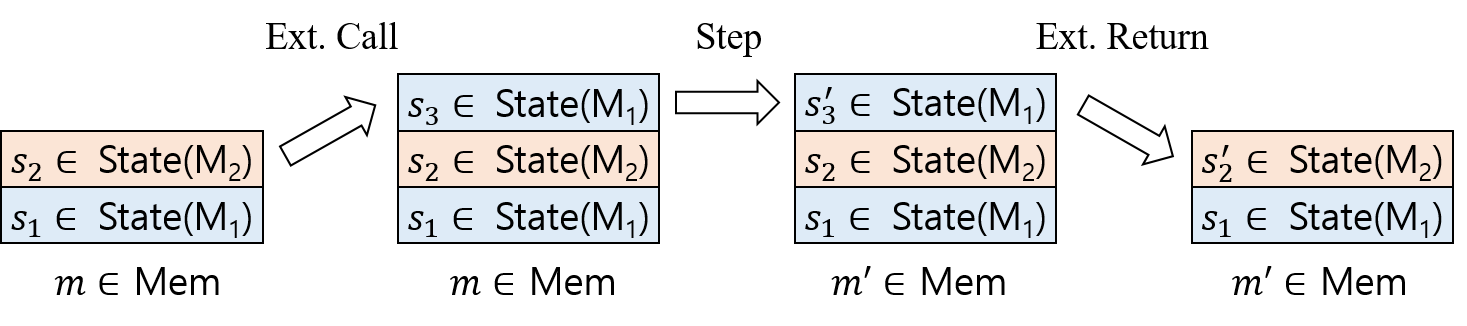
\includegraphics[width=0.9\linewidth]{images/intersem.png}
\caption{An execution of interaction semantics}
\label{fig:inter-sem}
\end{figure}

%% marshalling unmarshalling
%% marshalling the argument values into a list of values
%% setting the initial core states, unmarshalling the list of arguments.
%% at\_external: marshalling the argument values into a list of values
%% after\_external: unmarshalling the return value into
%% halted: marshalling the return value
%% corestep: use the underlying language semantics

Finally, note that the language semantics of C, assembly and
intermediate languages can be lifted to give a module semantics by
defining \texttt{corestep} to be the same as the execution step of the
language's semantics, and the other module operations to reflect the
calling conventions. Note also that all language-specific resources
(\ie other than the memory)
such as the register-file of assembly 
reside inside the module state, and thus are
duplicated at each invocation of a module.

%% One can lift a \cc{} language semantics into a core semantics by providing the interfaces:
%% Note that it is possible to define a core semantics using a mathematical specification.

\subsection{Problems}
\label{sec:overview-semantics:problems}

The problems with the interaction semantics of \ccc{} are that it does
not satisfy two adequacy properties. First, the adequacy w.r.t. C says
that for any C modules $M_1,\ldots,M_n$, the behaviors of the linked
program according to interaction semantics $\beh{M_1 \llink
  \ldots \llink M_n}$ should \emph{be included in} those according to the
physical semantics $\beh{M_1 \plink \ldots\plink M_n}$.  The reason for
failure was quite simple and we could easily fix it: unlike \ccc{}, we allow passing
the \texttt{undef} value to an external module since the C semantics
does so, while we turn ill-typed values into \texttt{undef} when they
are passed to an external module.

Second, the failure of the adequacy w.r.t. assembly is more serious.
Adequacy says that for any assembly modules $M_1,\ldots,M_n$,
the behaviors of the linked program according to interaction
semantics $\beh{M_1 \llink \ldots \llink M_n}$ should \emph{include}
those according to the physical semantics $\beh{M_1 \plink \ldots\plink M_n}$.
Note that the direction is opposite since assembly is the target language.
As discussed before, the reason for failure is that
the interaction semantics of \ccc{} does not have a mechanism to detect
illegal interference and make it undefined behavior~(UB).

%% A serious problem with the interaction semantics of \ccc{} is that it
%% is not correctly related to the physical assembly behavior. More
%% precisely, the behaviors of linked assembly modules according to
%% interaction semantics does not always include those according to \cc{}'s
%% assembly semantics, and in fact \ccc{} missed such a proof.

%% The problem is interference, which does not occur in the interaction
%% semantics due to logical isolation (ie, registers and argument area of
%% stack are not shared), but occurs in the physical behavior.

%% This problem, rather surprisingly, involves an essential and
%% challenging issue with linking with \emph{arbitrary} assembly
%% code. The issue is that arbitrary assembly code, unlike
%% compiler-generated assembly code, may break compilers' implicit
%% assumptions that their optimizations rely on.
%% \todo{make it clearer: Indeed \ccc{}'s
%% interaction semantics implicitly imposes such assumptions at
%% intermodule steps regardless of the actual behavior of assembly code.}
%% While this enables proving the optimizations correct, it makes the
%% interaction semantics deviate from the actual assembly semantics.
%%

\subsection{Our Solution}
\label{sec:overview-semantics:solution}

We identify the sources of inadequacy w.r.t. assembly as violations of
three assumptions made by standard compilers: two on the registers and one on the stack.
We discuss why they 
cause problems with counterexamples and show how to semantically
handle them without changing the underlying language semantics.

%% we figured out that there are three calling conventions that are the source of
%% the inadequacy
%% violation of CC does not affect the caller because interaction semantics gives isolation.
%% we have to give UB for those assembly code that violates calling conventions.
  
%% Our contribution: (i) identifying three kinds of such
%% interference and understanding them as violations of standard
%% calling conventions (ii) enhancing the wrapper semantics (without
%% changing the underlying language semantics at all) to give undefined
%% behavior to such interference, which requires nontrivial ideas as
%% we will see below. Explain the idea of undefined behavior (UB).

%% We solved the problem by identifying three such assumptions and
%% defining those behaviors breaking them as UB, which required
%% developing new techniques for semantics and verification.  We discuss
%% problems, challenges and our solutions about two assumptions on
%% register values in \Cref{sec:overview-semantics-register} and those
%% about the other assumption on stack values in
%% \Cref{sec:overview-semantics-memory}.

%% In the
%% subsequent sections, we discuss the assumptions, the challenges and
%% the solutions: two assumptions on register values in
%% \Cref{sec:overview-semantics-register} and one on memory
%% values in \Cref{sec:overview-semantics-memory}.

\subsubsection{Assumptions on the Registers}
\label{sec:overview-semantics-register}
%
The two problematic assumptions on the registers are that
an invoked assembly function $(i)$ should
preserve the initial values of the callee-save registers, and $(ii)$
should not access the memory via the leftover pointer values remaining
in those registers that are not involved in passing meaningful information to the callee,
which we henceforth call \emph{\nip{}} registers.
%% in those registers, which we call \emph{non-passing} registers,
%% that are not involved in passing information to the callee.
%% the \emph{non-passing} registers (\ie those registers not involved
%% in passing information to the callee).
%% We discuss these two conventions together because it is nontrivial to find a
%% single model that enforces both conventions at the same time.
%% \jeehoon{I don't understand the last sentence..}
%% \jeehoon{``\nip{}'': how about ``opaque''?}

\begin{figure}[t]
\fbox{\begin{minipage}{.8pc}\mbox{}\\[13.53mm](a)\\[11.73mm]\mbox{}\end{minipage}}
\hspace*{-1.9mm}
\begin{minipage}{0.55\textwidth}
\begin{Verbatim}[frame=single]
int main()   {          main:
  int* x = malloc(8);     ...
  x[0] = 0;               *(%rbx) = 0;
  x[1] = 1;               *(%rbx + 4) = 1;
  f();               -->  f();
  out(x[0]);              out(*(%rbx));
  ...                     ...
}
\end{Verbatim}
\end{minipage}
$\mbox{}~\mathlarger{\mathlarger{\mathlarger{\mathlarger{\mathlarger{\llink}}}}}~\mbox{}$
\fbox{\begin{minipage}{.8pc}\mbox{}\\[9.33mm](b)\\[7.53mm]\mbox{}\end{minipage}}
\hspace*{-1.9mm}
\begin{minipage}{0.28\textwidth}
\begin{Verbatim}[frame=single]
f:
  if (g(%rbx))
    %rbx = %rbx + 4;
  else
    *(%rbx) = 1;

\end{Verbatim}
\end{minipage}
\caption{A counterexample showing the problem with the assumptions on the registers}
\label{fig:reg-convention}
\end{figure}

\myparagraph{Counterexamples}
%
The example in \Cref{fig:reg-convention} shows how violations of the two
assumptions can invalidate correct compiler translations.
%% \jeehoon{I think counterexample should go to the problems section.}
%
The code in the left box~(a) shows a standard translation of C code into assembly
(written in pseudocode) performed by mainstream compilers like GCC and LLVM, where the accesses to
the array \texttt{x} are translated into accesses via the register
\texttt{\%rbx} assuming that \texttt{\%rbx} is set to contain the
address of \texttt{x}. An important point here is that the compiler
assumes that $(i)$ the value of \texttt{\%rbx} is unchanged across
the function call \texttt{f()} since it is a callee-save register,
and also $(ii)$ the values in the array pointed to by \texttt{\%rbx} are
unchanged across \texttt{f()} since the array's addresses do not escape
except via \nip{} registers like \texttt{\%rbx}.
Therefore, the compiler expects that \texttt{out(*(\%rbx))} in the target code
correctly outputs \texttt{0}.

The right box~(b) presents an example of handwritten assembly
(written in pseudocode) for function \texttt{f} that violates the
above two assumptions of the compiler. The code either increments
\texttt{\%rbx} by \texttt{4} or writes \texttt{1} to \texttt{*(\%rbx)}
depending on the result of call to \texttt{g}.  Now if we link the assembly
code in (a) and that in (b) together, one can easily see that
\texttt{out(*(\%rbx))} incorrectly outputs~\texttt{1} instead
of \texttt{0} in either case: in the former case, \texttt{\%rbx}
points to the second element of the array~\texttt{x}, which contains
\texttt{1}; in the latter case, the value of \texttt{*(\%rbx)} is
directly updated to \texttt{1}. Therefore, it makes sense to
define those illegal behaviors of (b) as undefined behavior~(UB).

\myparagraph{Our Model}
%
We present our model making the illegal behaviors UBs
in stages, explaining at each stage why naive models do not work.
%% \jeehoon{What's the difference between ``stage'' and ``state''?}
%% \jeehoon{We have ``Our Solution'' paragraph inside ``Our Solution'' subsection. How about moving
%%   counterexample to the problems subsection, and giving a paragraph to each stage?}

First, in order to enforce the preservation of callee-save register
values, we store the initial values of the callee-save registers at
the \texttt{init-core} step of assembly modules; and check, at the
\texttt{halted} step, whether the final values of those registers are
equal to the stored initial values and if not, raise UB.  Here, the
question is, when a new core with a fresh register file is pushed into the core stack,
what values should be set as initial values of the \nip{}
registers including all of the callee-save registers.  Since the
registers may contain arbitrary values in the physical assembly
semantics, a natural choice would be to initially set them to contain
the \texttt{undef} value, which is an abstract value representing all
possible values. Indeed, this is the choice of \ccc{}.  However, there
is a serious problem. Since, for instance, \texttt{undef + 4} results
in \texttt{undef}, checking whether the final values of callee-save
registers are equal to the initial values, \ie \texttt{undef}, is
not sufficient. Specifically, the assembly code in (b) above
does not raise UB in this new semantics in case \texttt{g(\%rbx)} returns \texttt{1}
because the initial and final values of \texttt{\%rbx}
are both \texttt{undef} and thus equal
even though the callee-save register \texttt{\%rbx} is incremented
by \texttt{4} in the physical semantics.

Second, another natural solution would be to initially set the
\nip{} registers to nondeterministically contain arbitrary
values including \texttt{undef}. Though this model is more flexible,
it still has a problem. For instance, in the above example, to
simulate the physical behaviors of the assembly function \texttt{f} in
interaction semantics, one can set the initial value of \texttt{\%rbx} to
be either $(i)$ \texttt{undef} (\ie a more abstract value than the physical one), or
$(ii)$ a pointer to the array \texttt{x} (\ie a value equivalent to the physical one):
other values cannot be used since they are not refined by the value of \texttt{\%rbx} in the target,
which is required since the value is passed to an unknown function~\texttt{g}.
In the former case, if
\texttt{g(\%rbx)} returns \texttt{1}, we have the same problem with
callee-save checking as shown above.  In the latter case, if
\texttt{g(\%rbx)} returns \texttt{0}, the function \texttt{f}
successfully updates the array~\texttt{x} thereby invaliding the
translation in (a) as illustrated above.

We solve this problem by further revising the second model:
nondeterministically allocating an arbitrary number of \emph{junk
  blocks} (\ie blocks of size zero) and then initializing the
\nip{} registers with arbitrary non-pointer values or
\emph{junk pointers} (\ie pointers to the junk blocks).  Then we can
simulate the physical behaviors by initializing each register $r$
$(i)$ with the same non-pointer value if the physical value of $r$ is
a non-pointer value; and $(ii)$ otherwise with a fresh junk pointer.
The high-level idea is that, like \texttt{undef}, a junk pointer is
more abstract (\ie causing more UBs) than any pointer but, unlike
\texttt{undef}, sufficiently distinguishable. For instance,
in the previous example, if \texttt{g(\%rbx)} returns \texttt{1},
the initial and final values of \texttt{\%rbx} (\ie $p$ and $p+4$ for a junk pointer $p$)
are distinguished thereby raising UB by the callee-save checking;
if \texttt{g(\%rbx)} returns \texttt{0},
the memory access \texttt{*(\%rbx) = 1} raises UB because \texttt{\%rbx}
points to a junk block of size zero.

Finally, note that introducing nondeterminism as above is not a
showstopper thanks to the mixed simulation, as discussed in
\Cref{sec:overview-verification:mixedsim}: we can do forward
simulation everywhere except for the \texttt{init\_core} step of
assembly modules, where we should do backward simulation.
%% there is one more technical problem: the model would prevent
%% the use of forward simulations due to the nondeterminism.  We solved
%% this problem by developing more general simulations, called
%% \emph{mixed simulations}, that (mostly) allow forward reasoning in the
%% (occasional) presence of nondeterminism (See \Cref{sec:main-verification:mixedsim} for details).

%% \todo{Say when returning, callee-save registers become \texttt{undef}.}

%% This model could possibly avoid the above
%% problem: in this new core semantics, \texttt{\%rbx} in the function
%% \texttt{f} can initially contain an equivalent value as in the
%% physical semantics, \ie a pointer to the array \texttt{x},
%% which gives more behaviors to the core semantics.
%% However, sensible choice that gives refinement is two, in the former, does not raise UB, in the latter also invalidates the compiler translation as .
%% in order to simulate
%% This could possibly solve the above problem: in this new core semantics, \texttt{\%rbx}
%% in the function \texttt{f} can initially contain an equivalent value as in the physical semantics,
%% \ie a pointer to the array \texttt{x},
%% in which case the
%% final value, when $\texttt{g(\%rbx)} = \texttt{1}$, would be
%% \texttt{4} and thus raise UB since $\texttt{4} \neq
%% \texttt{0}$. However, there are two problems. One is that this
%% semantics would prevent the use of forward simulations due to the
%% nondeterminism. We solved this problem by developing more general
%% simulations, called \emph{mixed simulations}, that (mostly) allow
%% forward reasoning in the (occasional) presence of nondeterminism (See
%% \Cref{sec:?} for details). The other, more essential, problem is that
%% it would be hard to prove that the core semantics of assembly code
%% like that in (b) is in general refined by its physical semantics.
%% To see this, consider the example in \Cref{fig:reg-convention} again, where in
%% the physical semantics \texttt{\%rbx} points to the array \texttt{x}
%% of \texttt{main} when \texttt{f} is called. In order to show the
%% refinement in this case, as an initial value of \texttt{\%rbx} in the
%% core semantics one can only sensibly choose, in general, either \texttt{undef},
%% a \emph{more abstract} value, or an \emph{equivalent} pointer pointing
%% to the address of \texttt{x} because \texttt{\%rbx} is passed to an
%% unknown function \texttt{g}. Then in the former case, if $\texttt{g(\%rbx)}$
%% returns \texttt{1}, no UB happens and \texttt{main} outputs \texttt{0}
%% in the core semantics since no registers are shared between different cores,
%% while \texttt{main} incorrectly outputs \texttt{1} in the physical semantics as shown above.
%% In the latter case, if $\texttt{g(\%rbx)}$ returns \texttt{0},
%% also no UB happens and 

\subsubsection{Assumptions on the Stack}
\label{sec:overview-semantics-memory}
%
The problematic assumption on the stack is that the
\emph{outgoing arguments area} of a caller's stack (\ie where overflowing function
arguments are stored) should be fully \emph{owned} by the callee. In
other words, the callee can assume that the arguments area is never
modified by others unless its addresses are revealed to the public by
the callee itself.

\begin{figure}[t]
\fbox{\begin{minipage}{.8pc}\mbox{}\\[9.33mm](a)\\[7.53mm]\mbox{}\end{minipage}}
\hspace*{-1.9mm}
\begin{minipage}{0.255\textwidth}
  \begin{Verbatim}[frame=single]
main:
  ...  
  leak = %rsp;
  f(..., 0);
g:
  *leak = 1;
  \end{Verbatim}
\end{minipage}
$\mbox{}~\mathlarger{\mathlarger{\mathlarger{\mathlarger{\mathlarger{\llink}}}}}~\mbox{}$
\fbox{\begin{minipage}{.8pc}\mbox{}\\[9.33mm](b)\\[7.53mm]\mbox{}\end{minipage}}
\hspace*{-1.9mm}
\begin{minipage}{0.595\textwidth}
  \begin{Verbatim}[frame=single]
void f(..., int64_t x)       f:
{                              ...
  out(x);                      out(*(%rax));
  g();                  -->    g();
  out(x);                      out(*(%rax));
}                              ...
  \end{Verbatim}
\end{minipage}
\\[1mm]
\fbox{\begin{minipage}{.8pc}\mbox{}\\[17.53mm](c)\\[16.73mm]\mbox{}\end{minipage}}
\hspace*{-1.9mm}
\begin{minipage}{.95\textwidth}
\fbox{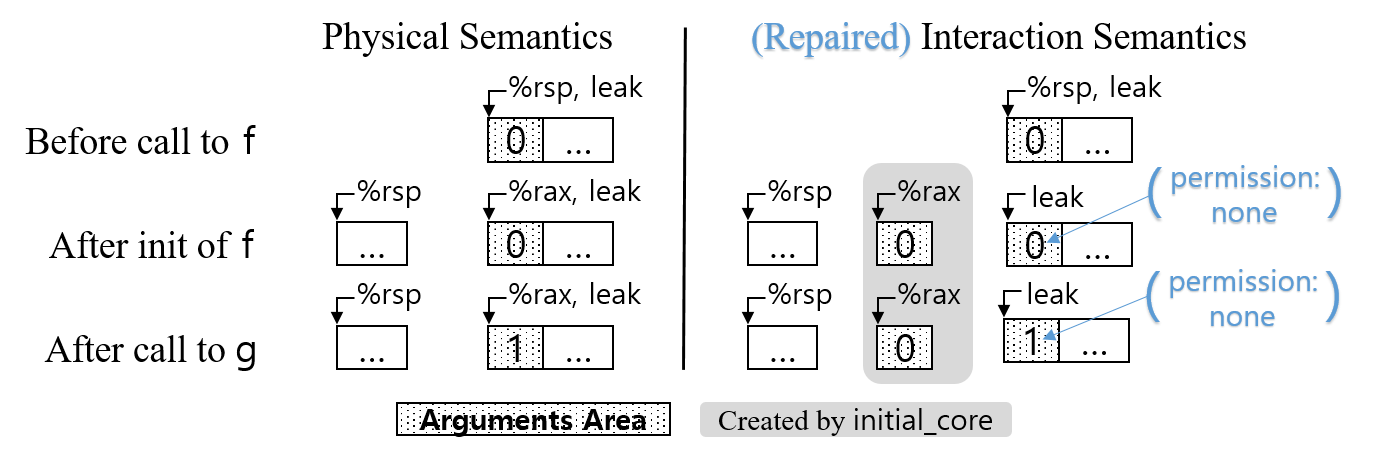
\includegraphics[width=.983\textwidth]{images/ex-stack.png}}
\end{minipage}
%% \fbox{\begin{minipage}{.8pc}\mbox{}\\[4.53mm](c)\\[3.73mm]\mbox{}\end{minipage}}
%% \hspace*{-1.9mm}
%% \begin{minipage}{.95\textwidth}
%%   \begin{Verbatim}[frame=single]
%%                      Physical Semantics         Interaction Semantics
%%                             %rsp           |                  %rsp       
%% Before call to f:           [=0=| ... ]    |                  [=0=| ... ]
%%                     %rsp    %rax           |    %rsp    %rax             
%%  After init of f:   [ ... ] [=0=| ... ]    |    [ ... ] [=0=] [=0=| ... ]
%%                     %rsp    %rax           |    %rsp    %rax             
%%  After call to g:   [ ... ] [=1=| ... ]    |    [ ... ] [=0=] [=1=| ... ]
%%   \end{Verbatim}
%% \end{minipage}
\caption{A counterexample showing the problem with the assumption on the stack}
\label{fig:stack-convention}
\end{figure}

\myparagraph{Counterexamples}
%
The example in \Cref{fig:stack-convention} shows how violations of the assumption
can invalidate correct compiler translations.
%
The box~(a) shows handwritten assembly code implementing two functions
\texttt{main} and \texttt{g}; the box~(b) shows a standard translation
of C code into assembly essentially performed by \texttt{gcc -O0}; and
the left-hand side (LHS) of the box~(c) depicts the shape of the stack
during execution in the physical semantics.
The function \texttt{main} stores the address of the
outgoing arguments area (\ie \texttt{\%rsp} as depicted in LHS of (c))
in the global variable \texttt{leak} and invokes the function
\texttt{f}, where the last argument \texttt{0} is stored in the
arguments area of the stack. Then the function \texttt{f} makes three
function calls, \texttt{out(x)}, \texttt{g()} and \texttt{out(x)},
where the argument \texttt{x} is directly read from the arguments area
pointed to by \texttt{\%rax} in the assembly, as depicted in LHS of
(c), and \texttt{out(x)} outputs the read value.  Finally, the
function \texttt{g} updates the arguments area pointed to by
\texttt{leak} with~\texttt{1}, as depicted in LHS of (c), between the
two function calls \texttt{out(x)}.

An important point here is that the compiler assumes that the
arguments area (\ie \texttt{\%rax}) is unchanged across the
function call \texttt{g()} since it is fully owned by \texttt{f}.
Therefore, the compiler expects that both calls
\texttt{out(*(\%rax))} in the target code correctly output
\texttt{0}. However, since the function \texttt{g} updates the
arguments area with \texttt{1} via \texttt{leak}, the two calls
incorrectly output \texttt{0} and~\texttt{1}.
We confirmed this incorrectness by
compiling \texttt{f} with \texttt{gcc -O2}, which
eliminates the second load \texttt{*(\%rax)} by propagating
the result of the first load across \texttt{g()}
thereby outputting \texttt{0} twice.

\myparagraph{Our Model}
%
In order to solve the problem, we have to distinguish accesses to the
arguments area via the caller from those via the callee and define the
former as UB. Though making such distinction is difficult in the
physical semantics, fortunately it is already made in interaction
semantics due to the language-independent design. For example, consider
the interaction semantics of the above example, depicted in the
right-hand-side (RHS) of \Cref{fig:stack-convention}~(c).  The
difference is that when the assembly function \texttt{f} is invoked,
the initialization process (\ie \texttt{init\_core}) of the module
semantics newly constructs the arguments area of the stack from the
given logical arguments in order to make an environment needed to
execute the assembly function \texttt{f}. This is essentially needed
because the caller may not be an assembly module so that it may not
have its own stack at all.  Then the callee sees the new arguments
area created by \texttt{init\_core} while the caller (in assembly)
sees the original arguments area.

Although the original interaction semantics does not prevent access to
the arguments area via the caller, we can easily fix it.
%% Now we can easily repair the original interaction semantics to make
%% those accesses to the arguments area via the caller as UB during the
%% lifetime of the callee.
We simply $(i)$ turn off the access
permission of the original arguments area in the \texttt{at\_external}
step of the caller module, and $(ii)$ turn it back on in the
\texttt{after\_external} step. Note that the notion of permission
%% is already an existing feature of
already exists in the \cc{} semantics, so that we do not
need to strengthen it. In the above example again,
the update by \texttt{g} will raise UB since the original argument area pointed
to by \texttt{leak} has no access permission.

%% \jeehoon{I think the idea of repairing interaction semantics is a little bit abrupt.  I think it's
%%   necessary to explain why interaction semantics is wrong.}

\hide{

\todo{Interaction Semantics and UB}

\myparagraph{Correctness Statement}
%
\ccc{}'s correctness also establishes behavioral refinement. To be
specific, consider a source program consisting of C modules
$\texttt{s}_1\texttt{.c},\ldots,\texttt{s}_n\texttt{.c}$ and assembly
modules $\texttt{a}_1\texttt{.asm},\ldots,\texttt{a}_m\texttt{.asm}$.
Now suppose
$\texttt{t}_1\texttt{.asm},\ldots,\texttt{t}_n\texttt{.asm}$ are the
assembly modules separately compiled from the source C modules by the
\cc{} compiler. The correctness of this compilation says that the
observable behaviors of the target assembly consisting of
$\texttt{t}_1\texttt{.asm},\ldots,\texttt{t}_n\texttt{.asm}$,
$\texttt{a}_1\texttt{.asm},\ldots,\texttt{a}_m\texttt{.asm}$ is
included in that of the source program according to \emph{interaction
  semantics} described below.

\begin{figure}[t]%% {0.43\textwidth}
  \centering
  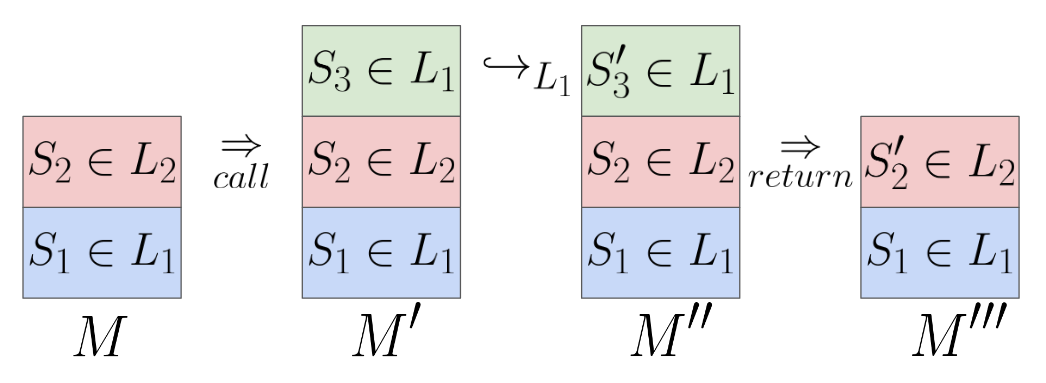
\includegraphics[width=0.7\linewidth]{images/interaction-semantics2.png}
  \caption{}
\label{fig:interactionsemantics}
\end{figure}

Interaction semantics gives a mathematical model for executing
multi-language programs by providing a general mechanism that defines
intermodule steps, while defining intramodule steps according to the
underlying language's semantics.
\todo{
  revise the following: main points
  - copying module states for generality
  - C, assembly, ILs share the same notion of memory
  - marshalling, unmarshalling and making environment for the module (the underlying language assumes the uni-language setting.) --> change memory at intermodule steps
}
%
\Cref{fig:interactionsemantics} illustrates how interaction semantics works.
%% As illustrated in \Cref{fig:interactionsemantics},
The state of interaction semantics consists of a \emph{shared} memory, and a stack of language-local states \emph{without} memory.
The notion of shared memory is legitimate because every language of \cc{} shares the same notion of memory.
%% Note that every language of \cc{} shares the notion of memory, and hereafter we use $\States{\mathbb{L}}$ to denote a language-local state \emph{without} memory (\eg local variable mapping for C and register set for assembly).
Intermodule steps pushes or pops the stack (at call case and return case, respectively) while intramodule steps just changes the topmost state of the stack.
%% Intermodule steps are divided into two kinds, namely call and return, each pushing and popping the stack.
%% Intramodule steps does not push or pop the stack, instead it just updates the topmost state of the stack.
%% \Cref{fig:interactionsemantics} illustrates these in more detail.

\youngju{multi-language program? multi-module program?}

%% During its execution, $S_2$ encounters a call to an external function.
Note that, in order to define intermodule steps modularly, a representation of function arguments is globally fixed ($\overrightarrow{val}$).
Therefore, when $S_2$ encounters a call to an external function, $L_2$ \emph{marshall}s arguments from its language-local representation to global representation before passing them.
Then $L_3$ receives the arguments and \emph{unmarshall}s those to its language-local representation and initializes a new state with it, resulting in $S_3$.
An intramodule step of $S_3$ proceeds by just reusing its language-local step, $\estep{}_3$.
When $S_3'$ returns, similarly with call case, the return value is passed to $S_2$ (through marshalling and unmarshalling) and its state is updated correspondingly.


%% ($S_i \in \States{\mathbb{L}_i}$)

%% The left arrow and right arrow each depicts intermodule step,
%% When a function from another module is called during its execution,
%% During its execution, a function from another module is called during execution, a new
%% $S_2$
%% When an external module is called,
%% There are two kinds of intermodule steps, namely call and return, each pushing and popping
%% \youngju{처음부터 memory 분리?}
%% the intermodule step is divided into \emph{call} and \emph{return}, each pushing or popping
%% As illustrated in \Cref{fig:interactionsemantics}, the intermodule step is divided into \emph{call} and \emph{return}, each pushing or popping

\todo{Discuss advantages of interaction semantics, here or intro?}

\subsection{Semantic Techniques}\label{sec:background:ub}

Common compiler optimizations are not always correct in general for
all well-typed C programs because the syntactic type checking cannot
rule out all semantically invalid programs. In order to rule out such
invalid programs thereby making those optimizations correct, \cc{}
uses two semantic techniques, \emph{undefined behavior} and
\emph{logical memory}. In addition, to model uninitialized values,
\cc{} uses the notion of \emph{undefined value}.

\myparagraph{Undefined Behavior}
%
The main idea for ruling out invalid programs is to raise
\emph{undefined behavior (UB)} during execution if an undesirable
operation occurs, where UB is interpreted as producing all possible
traces of events.  Then for correctness of optimizations, it suffices
to prove behavioral refinement until UB happens because, once it
happens, behavioral refinement holds trivially.
As an example, consider the following program.
%
\[
\begin{minipage}{0.4\textwidth}
\begin{verbatim}
int arr[1], x = 0;
*(arr+1) = 1;
out(x); // optimizes to "out(0)"
\end{verbatim}
\end{minipage}
\]
%
Here \cc{} optimizes \texttt{out(x)} to \texttt{out(0)} by
propagating the initial value of \texttt{x} because a simple analysis
indicates that the variable \texttt{x} is not modified.  However, this
analysis would be invalidated in a naive semantics.  For example,
suppose \texttt{arr} and \texttt{x} are allocated at \texttt{0x100}
and \texttt{0x104}. Then the out-of-bound access \texttt{*(arr+1) = 1}
updates \texttt{x} with \texttt{1} thereby making the optimization
incorrect.  \cc{} solves this problem by defining such out-of-bound
access as undefined behavior.

Now the question is how to define out-of-bound access. To see the
problem, consider the two accesses \texttt{*(arr+1)} and \texttt{*(\&x)}
in the above example. Though \texttt{arr+1} and \texttt{\&x} are exactly
the same address \texttt{0x104}, one should be able to distinguish them:
the former access as out-of-bound but the latter not.

%% As an example,
%% consider a simple optimization translating \texttt{x+1 > x} to
%% \texttt{true}. \todo{revise:}
%% Note that if \code{x} was \code{INT\_MAX}, the inequality does not hold because of an integer overflow.
%% Therefore, such invalid operation (triggering overflow) is defined as UB so that the optimization is justified.

\myparagraph{Logical Memory}
%
To address this problem, \cc{} introduces the notion of \emph{logical
  memory}, which models the memory as a set of independent blocks and
pointer values as pairs of a block identifier and an offset inside the
block. In the previous example, two logical blocks of size 1 are
allocated: one for \texttt{arr} with identifier, say \texttt{bid 10},
and the other for \texttt{x} with identifier, say \texttt{bid
  11}. Then the addresses \texttt{arr+1} and \texttt{\&x} are
distinguished as \texttt{(bid 10,1)} and \texttt{(bid 11,0)}, where
the former is clearly out-of-bound but the latter not because the
blocks are of size 1.

%% \youngju{전달할 이야기: (i) private protection이 중요 (ii) 메모리 기본 연산들 (alloc, free) 이 동작하는 방식? (marshall/unmarshall)}

%% \youngju{invalid access 라고 뭉뚱그려 말한 이유: dangling pointer 등도 UB를 잘 준다.}

%% \youngju{free 설명할 때 dangling pointer로 설명?}

%% \youngju{https://hal.inria.fr/hal-00703441/document 보고 써서 문장이 비슷한데 paraphrase 더 해야 할 수도}

%% \youngju{여기만 생각하면 separation만 가지고 설명해도 충분한데, 위에서 out-of-bound access 이야기랑 맞춰야 함}

%% \youngju{primitive operation 이야기: 우리는 하나 늘린 셈 (unfree). 이게 장점인지 단점인지}

%% \youngju{alloc이 사실은 Z 두개 받는데, \Cref{fig:logical-memory}랑 안헷갈리게 하나로 함}

\myparagraph{Undefined Value}
%
\todo{
  - uninitialized value -> undefined value
  - undefined value -> propagate; observe on UV -> UB
  - As a result, one can optimize UV to any value.
  - Note that modeling uninitialized value as assigning arbitrary values nondeterministically
    or branching on UV as branching either way nondeterministically
    is not an option for \cc{} because the language should deterministic in order to use forward simulation as discussed in Section blah.
}


} %\hide 

\hide{

\subsection{Applications}

%% The root cause of such overhead is that their verification technique
%% was not flexible: a single memory relation is enforced for every
%% per-pass correctness proof. In contrast, \cc{} employs three different
%% memory relations so that each pass can be proven with the simplest but
%% sufficient one. In other words, their approach failed to achieve
%% \emph{true vertical compositionality}\cite{TODO}.

%% To address this problem, we developed new proof techniques that allow
%% lightweight verification with focus on minimizing language-specific
%% and pass-specific developments. First one is end-language contextual
%% refinement, which recovers the flexibility to chose a convenient
%% memory relation. Second one is mixed simulation, which tames the
%% nondeterminism introduced in \Cref{sec:overview-semantics}. The last
%% one is an analysis framework to address a new challenge about modular
%% verification of modular analysis. \todo{why new? introduced recently}

To address this problem, we developed new proof techniques that allow
lightweight verification with focus on minimizing language-specific
and pass-specific developments. First one is end-language contextual
refinement, which addresses the root cause of \ccc{}'s overhead:
vertical composition (of simulation relation).
%% it
%% fixed \emph{single}, sophisticated memory relation for every per-pass
%% proof, while \cc{} employs three different ones so that each per-pass
%% proof uses sufficient but simplest one.
Second one is mixed simulation, which tames the nondeterminism we
introduced in \Cref{sec:overview-semantics}. The last one is a local
preservation, which supports verification of modular analysis which
was introduced in \cc{} since \ccc{} was no longer maintained.

As a result, we successfully reused \cc{}'s developments and our
development comprises 48K lines of Coq (25.4\% compared to the
baseline) where language-specific or pass-specific developments are
only 11K lines of Coq (13.3\% compared to corresponding baseline).
%order-of-magnitue smaller?

\vspace{5mm}
\begin{tabular}{ c || c | c || c | c }
  portion
  &
  \ccc{}
  &
  \cc{} 2.1
  &
  \ccm{}
  &
  \cc{} 3.5
  \\
  \hline
  language/pass-specific
  &
  +76,973 (125.8\%)
  &
  61,196
  &
  +11,339 (13.3\%)
  &
  85,056
  %% \\
  %% others (TODO: remove?)
  %% &
  %% +45,304
  %% &
  %% 50,925
  %% &
  %% +36,956
  %% &
  %% 105,048
  \\
  whole
  &
  +122,277 (109.1\%)
  &
  112,125
  &
  +48,295 (25.4\%)
  &
  190,104
\end{tabular}
\vspace{5mm}

As a consequence, the intermodule case of the local simulation can be
established \emph{assuming} the source state is sound (just as in
whole-program simulation), as the preservation of sound-state is
provided by local-preservation. Of course, the horizontal composition
of local simulations now additionally require local preservations of
each end language, which will actually be just C, RTL (a target
language of analyzers), and assembly thanks to ELCR.

\note{without ./bounds/, 41424}

\note{counted only x86 directory. should we mention it?}

\note{v3.5 has parser.v (34083 LOC) and v2.1 does not.}

\todo{1,000 or 1000?}

\todo{show the number without Stackingproof.v?}



\todo{위: re-implementation of each language’s semantics and each passes’ proof
  아래: language-specific or pass-specific developments}

%쓰이는 표현임: Not by Power, Nor by Might, but by My Spirit
%lines of Coq: sepcomp에서 쓰임
%evolve over time 쓰임
%In response: viktor abstract에서 씀
%10331.0 / 79488

\todo{
Except for the initial state, every other state remains deterministic,
and we were able to reuse existing proof at ease.  As a consequence,
we successfully reused existing proof.
}








%% 우리가 추가한 nondeterminisim은 오직 assembly가 시작할 때 뿐이고, 나머지 부분은 여전히 deterministic하다.
%% 이 local determinisim을 이용해서 2-b)로 논증하면, 기존 forward simulation을 성공적으로 재사용할 수 있다.




\subsection{Defining a Sound and General Semantics}\label{sec:overview:semantics}
In this subsection, we describe challenges on defining a sound and general multi-language semantics for C and assembly, and show our solution.
By \textit{sound}, we mean its behavior contains actual behavior when ran on the machine.
By \textit{general}, we mean it should support arbitrary program.
%% that is \textit{general}, \eg{} supporting \textit{arbitrary}
We elide some technical subtleties for the sake of simplicity.
In \Cref{TODO}, we provide technically more complete argument for a curious reader.

\subsection{Register (tentative)}\label{sec:overview:register}
\myparagraph{Problem (tentative)}
%% %% \chapter{\;\;\;\;Compiler Verification: CompCertM} %%이러면 (toc 말고 본문에서) 넘침
\chapter{\;\;\;\;Compiler Verification}
\label{sec:compiler}

\section{Background}
\label{sec:compiler:background}

\subsection{A Brief Introduction on CompCert}

\myparagraph{Undefined Behavior}



\section{Problems}
\label{sec:compiler:problems}

The problems with the interaction semantics of \ccc{} are that it does
not satisfy two adequacy properties. First, the adequacy w.r.t. C says
that for any C modules $M_1,\ldots,M_n$, the behaviors of the linked
program according to interaction semantics $\beh{M_1 \llink
  \ldots \llink M_n}$ should \emph{be included in} those according to the
physical semantics $\beh{M_1 \plink \ldots\plink M_n}$.  The reason for
failure was quite simple and we could easily fix it: unlike \ccc{}, we allow passing
the \texttt{undef} value to an external module since the C semantics
does so, while we turn ill-typed values into \texttt{undef} when they
are passed to an external module.

Second, the failure of the adequacy w.r.t. assembly is more serious.
Adequacy says that for any assembly modules $M_1,\ldots,M_n$,
the behaviors of the linked program according to interaction
semantics $\beh{M_1 \llink \ldots \llink M_n}$ should \emph{include}
those according to the physical semantics $\beh{M_1 \plink \ldots\plink M_n}$.
Note that the direction is opposite since assembly is the target language.
As discussed before, the reason for failure is that
the interaction semantics of \ccc{} does not have a mechanism to detect
illegal interference and make it undefined behavior~(UB).

\section{Solution}
\label{sec:compiler:solution}

We identify the sources of inadequacy w.r.t. assembly as violations of
three assumptions made by standard compilers: two on the registers and one on the stack.
We discuss why they 
cause problems with counterexamples and show how to semantically
handle them without changing the underlying language semantics.

\subsection{Assumptions on the Registers}
\label{sec:overview-semantics-register}
%
The two problematic assumptions on the registers are that
an invoked assembly function $(i)$ should
preserve the initial values of the callee-save registers, and $(ii)$
should not access the memory via the leftover pointer values remaining
in those registers that are not involved in passing meaningful information to the callee,
which we henceforth call \emph{\nip{}} registers.
%% in those registers, which we call \emph{non-passing} registers,
%% that are not involved in passing information to the callee.
%% the \emph{non-passing} registers (\ie those registers not involved
%% in passing information to the callee).
%% We discuss these two conventions together because it is nontrivial to find a
%% single model that enforces both conventions at the same time.
%% \jeehoon{I don't understand the last sentence..}
%% \jeehoon{``\nip{}'': how about ``opaque''?}

\begin{figure}[t]
\fbox{\begin{minipage}{.9pc}\mbox{}\\[15.25mm](a)\\[13.45mm]\mbox{}\end{minipage}}
\hspace*{-2.7mm}
\begin{minipage}{0.70\textwidth}
\begin{Verbatim}[frame=single]
int main()   {          main:
  int* x = malloc(8);     ...
  x[0] = 0;               *(%rbx) = 0;
  x[1] = 1;               *(%rbx + 4) = 1;
  f();               -->  f();
  out(x[0]);              out(*(%rbx));
  ...                     ...
}
\end{Verbatim}
\end{minipage}
$\mbox{}~\mathlarger{\mathlarger{\mathlarger{\mathlarger{\mathlarger{\llink}}}}}~\mbox{}$
\\
\vspace{3mm}
\\
\fbox{\begin{minipage}{.9pc}\mbox{}\\[10.50mm](b)\\[8.70mm]\mbox{}\end{minipage}}
\hspace*{-2.7mm}
\begin{minipage}{0.33\textwidth}
\begin{Verbatim}[frame=single]
f:
  if (g(%rbx))
    %rbx = %rbx + 4;
  else
    *(%rbx) = 1;

\end{Verbatim}
\end{minipage}
\caption{A counterexample showing the problem with the assumptions on the registers}
\label{fig:reg-convention}
\end{figure}

\myparagraph{Counterexamples}
%
The example in \Cref{fig:reg-convention} shows how violations of the two
assumptions can invalidate correct compiler translations.
%% \jeehoon{I think counterexample should go to the problems section.}
%
The code in the left box~(a) shows a standard translation of C code into assembly
(written in pseudocode) performed by mainstream compilers like GCC and LLVM, where the accesses to
the array \texttt{x} are translated into accesses via the register
\texttt{\%rbx} assuming that \texttt{\%rbx} is set to contain the
address of \texttt{x}. An important point here is that the compiler
assumes that $(i)$ the value of \texttt{\%rbx} is unchanged across
the function call \texttt{f()} since it is a callee-save register,
and also $(ii)$ the values in the array pointed to by \texttt{\%rbx} are
unchanged across \texttt{f()} since the array's addresses do not escape
except via \nip{} registers like \texttt{\%rbx}.
Therefore, the compiler expects that \texttt{out(*(\%rbx))} in the target code
correctly outputs \texttt{0}.

The right box~(b) presents an example of handwritten assembly
(written in pseudocode) for function \texttt{f} that violates the
above two assumptions of the compiler. The code either increments
\texttt{\%rbx} by \texttt{4} or writes \texttt{1} to \texttt{*(\%rbx)}
depending on the result of call to \texttt{g}.  Now if we link the assembly
code in (a) and that in (b) together, one can easily see that
\texttt{out(*(\%rbx))} incorrectly outputs~\texttt{1} instead
of \texttt{0} in either case: in the former case, \texttt{\%rbx}
points to the second element of the array~\texttt{x}, which contains
\texttt{1}; in the latter case, the value of \texttt{*(\%rbx)} is
directly updated to \texttt{1}. Therefore, it makes sense to
define those illegal behaviors of (b) as undefined behavior~(UB).

\myparagraph{Our Model}
\label{sec:compiler:solution:model}
%
We present our model making the illegal behaviors UBs
in stages, explaining at each stage why naive models do not work.
%% \jeehoon{What's the difference between ``stage'' and ``state''?}
%% \jeehoon{We have ``Our Solution'' paragraph inside ``Our Solution'' section. How about moving
%%   counterexample to the problems section, and giving a paragraph to each stage?}

First, in order to enforce the preservation of callee-save register
values, we store the initial values of the callee-save registers at
the \texttt{init-core} step of assembly modules; and check, at the
\texttt{halted} step, whether the final values of those registers are
equal to the stored initial values and if not, raise UB.  Here, the
question is, when a new core with a fresh register file is pushed into the core stack,
what values should be set as initial values of the \nip{}
registers including all of the callee-save registers.  Since the
registers may contain arbitrary values in the physical assembly
semantics, a natural choice would be to initially set them to contain
the \texttt{undef} value, which is an abstract value representing all
possible values. Indeed, this is the choice of \ccc{}.  However, there
is a serious problem. Since, for instance, \texttt{undef + 4} results
in \texttt{undef}, checking whether the final values of callee-save
registers are equal to the initial values, \ie \texttt{undef}, is
not sufficient. Specifically, the assembly code in (b) above
does not raise UB in this new semantics in case \texttt{g(\%rbx)} returns \texttt{1}
because the initial and final values of \texttt{\%rbx}
are both \texttt{undef} and thus equal
even though the callee-save register \texttt{\%rbx} is incremented
by \texttt{4} in the physical semantics.

Second, another natural solution would be to initially set the
\nip{} registers to nondeterministically contain arbitrary
values including \texttt{undef}. Though this model is more flexible,
it still has a problem. For instance, in the above example, to
simulate the physical behaviors of the assembly function \texttt{f} in
interaction semantics, one can set the initial value of \texttt{\%rbx} to
be either $(i)$ \texttt{undef} (\ie a more abstract value than the physical one), or
$(ii)$ a pointer to the array \texttt{x} (\ie a value equivalent to the physical one):
other values cannot be used since they are not refined by the value of \texttt{\%rbx} in the target,
which is required since the value is passed to an unknown function~\texttt{g}.
In the former case, if
\texttt{g(\%rbx)} returns \texttt{1}, we have the same problem with
callee-save checking as shown above.  In the latter case, if
\texttt{g(\%rbx)} returns \texttt{0}, the function \texttt{f}
successfully updates the array~\texttt{x} thereby invaliding the
translation in (a) as illustrated above.

We solve this problem by further revising the second model:
nondeterministically allocating an arbitrary number of \emph{junk
  blocks} (\ie blocks of size zero) and then initializing the
\nip{} registers with arbitrary non-pointer values or
\emph{junk pointers} (\ie pointers to the junk blocks).  Then we can
simulate the physical behaviors by initializing each register $r$
$(i)$ with the same non-pointer value if the physical value of $r$ is
a non-pointer value; and $(ii)$ otherwise with a fresh junk pointer.
The high-level idea is that, like \texttt{undef}, a junk pointer is
more abstract (\ie causing more UBs) than any pointer but, unlike
\texttt{undef}, sufficiently distinguishable. For instance,
in the previous example, if \texttt{g(\%rbx)} returns \texttt{1},
the initial and final values of \texttt{\%rbx} (\ie $p$ and $p+4$ for a junk pointer $p$)
are distinguished thereby raising UB by the callee-save checking;
if \texttt{g(\%rbx)} returns \texttt{0},
the memory access \texttt{*(\%rbx) = 1} raises UB because \texttt{\%rbx}
points to a junk block of size zero.

Finally, note that introducing nondeterminism as above is not a
showstopper thanks to the mixed simulation, as discussed in
\Cref{sec:overview-verification:mixedsim}: we can do forward
simulation everywhere except for the \texttt{init\_core} step of
assembly modules, where we should do backward simulation.

\subsection{Assumptions on the Stack}
\label{sec:overview-semantics-memory}
%
The problematic assumption on the stack is that the
\emph{outgoing arguments area} of a caller's stack (\ie where overflowing function
arguments are stored) should be fully \emph{owned} by the callee. In
other words, the callee can assume that the arguments area is never
modified by others unless its addresses are revealed to the public by
the callee itself.

\begin{figure}[t]
\fbox{\begin{minipage}{.9pc}\mbox{}\\[10.45mm](a)\\[8.65mm]\mbox{}\end{minipage}}
\hspace*{-1.9mm}
\begin{minipage}{0.255\textwidth}
  \begin{Verbatim}[frame=single]
main:
  ...  
  leak = %rsp;
  f(..., 0);
g:
  *leak = 1;
  \end{Verbatim}
\end{minipage}
$\mbox{}~\mathlarger{\mathlarger{\mathlarger{\mathlarger{\mathlarger{\llink}}}}}~\mbox{}$
\fbox{\begin{minipage}{.9pc}\mbox{}\\[10.45mm](b)\\[8.65mm]\mbox{}\end{minipage}}
\hspace*{-1.9mm}
\begin{minipage}{0.695\textwidth}
  \begin{Verbatim}[frame=single]
void f(..., int64_t x)       f:
{                              ...
  out(x);                      out(*(%rax));
  g();                  -->    g();
  out(x);                      out(*(%rax));
}                              ...
  \end{Verbatim}
\end{minipage}
\\[1mm]
\fbox{\begin{minipage}{.9pc}\mbox{}\\[15.90mm](c)\\[15.10mm]\mbox{}\end{minipage}}
\hspace*{-2.7mm}
\begin{minipage}{.95\textwidth}
\fbox{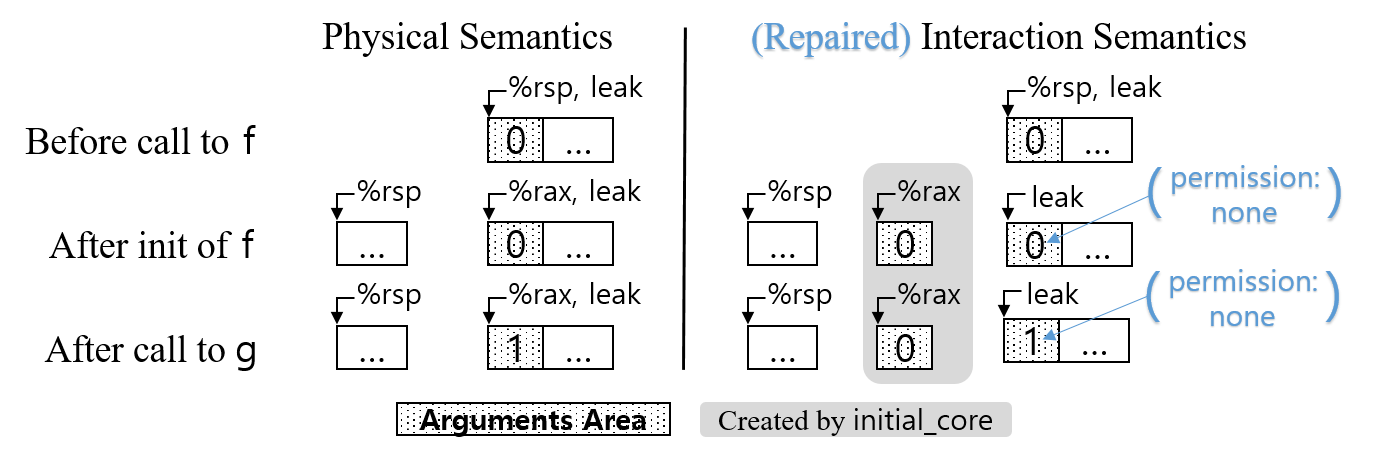
\includegraphics[width=.983\textwidth]{images/ex-stack.png}}
\end{minipage}
%% \fbox{\begin{minipage}{.8pc}\mbox{}\\[4.53mm](c)\\[3.73mm]\mbox{}\end{minipage}}
%% \hspace*{-1.9mm}
%% \begin{minipage}{.95\textwidth}
%%   \begin{Verbatim}[frame=single]
%%                      Physical Semantics         Interaction Semantics
%%                             %rsp           |                  %rsp       
%% Before call to f:           [=0=| ... ]    |                  [=0=| ... ]
%%                     %rsp    %rax           |    %rsp    %rax             
%%  After init of f:   [ ... ] [=0=| ... ]    |    [ ... ] [=0=] [=0=| ... ]
%%                     %rsp    %rax           |    %rsp    %rax             
%%  After call to g:   [ ... ] [=1=| ... ]    |    [ ... ] [=0=] [=1=| ... ]
%%   \end{Verbatim}
%% \end{minipage}
\caption{A counterexample showing the problem with the assumption on the stack}
\label{fig:stack-convention}
\end{figure}

\myparagraph{Counterexamples}
%
The example in \Cref{fig:stack-convention} shows how violations of the assumption
can invalidate correct compiler translations.
%
The box~(a) shows handwritten assembly code implementing two functions
\texttt{main} and \texttt{g}; the box~(b) shows a standard translation
of C code into assembly essentially performed by \texttt{gcc -O0}; and
the left-hand side (LHS) of the box~(c) depicts the shape of the stack
during execution in the physical semantics.
The function \texttt{main} stores the address of the
outgoing arguments area (\ie \texttt{\%rsp} as depicted in LHS of (c))
in the global variable \texttt{leak} and invokes the function
\texttt{f}, where the last argument \texttt{0} is stored in the
arguments area of the stack. Then the function \texttt{f} makes three
function calls, \texttt{out(x)}, \texttt{g()} and \texttt{out(x)},
where the argument \texttt{x} is directly read from the arguments area
pointed to by \texttt{\%rax} in the assembly, as depicted in LHS of
(c), and \texttt{out(x)} outputs the read value.  Finally, the
function \texttt{g} updates the arguments area pointed to by
\texttt{leak} with~\texttt{1}, as depicted in LHS of (c), between the
two function calls \texttt{out(x)}.

An important point here is that the compiler assumes that the
arguments area (\ie \texttt{\%rax}) is unchanged across the
function call \texttt{g()} since it is fully owned by \texttt{f}.
Therefore, the compiler expects that both calls
\texttt{out(*(\%rax))} in the target code correctly output
\texttt{0}. However, since the function \texttt{g} updates the
arguments area with \texttt{1} via \texttt{leak}, the two calls
incorrectly output \texttt{0} and~\texttt{1}.
We confirmed this incorrectness by
compiling \texttt{f} with \texttt{gcc -O2}, which
eliminates the second load \texttt{*(\%rax)} by propagating
the result of the first load across \texttt{g()}
thereby outputting \texttt{0} twice.

\myparagraph{Our Model}
%
In order to solve the problem, we have to distinguish accesses to the
arguments area via the caller from those via the callee and define the
former as UB. Though making such distinction is difficult in the
physical semantics, fortunately it is already made in interaction
semantics due to the language-independent design. For example, consider
the interaction semantics of the above example, depicted in the
right-hand-side (RHS) of \Cref{fig:stack-convention}~(c).  The
difference is that when the assembly function \texttt{f} is invoked,
the initialization process (\ie \texttt{init\_core}) of the module
semantics newly constructs the arguments area of the stack from the
given logical arguments in order to make an environment needed to
execute the assembly function \texttt{f}. This is essentially needed
because the caller may not be an assembly module so that it may not
have its own stack at all.  Then the callee sees the new arguments
area created by \texttt{init\_core} while the caller (in assembly)
sees the original arguments area.

Although the original interaction semantics does not prevent access to
the arguments area via the caller, we can easily fix it.
%% Now we can easily repair the original interaction semantics to make
%% those accesses to the arguments area via the caller as UB during the
%% lifetime of the callee.
We simply $(i)$ turn off the access
permission of the original arguments area in the \texttt{at\_external}
step of the caller module, and $(ii)$ turn it back on in the
\texttt{after\_external} step. Note that the notion of permission
%% is already an existing feature of
already exists in the \cc{} semantics, so that we do not
need to strengthen it. In the above example again,
the update by \texttt{g} will raise UB since the original argument area pointed
to by \texttt{leak} has no access permission.


\subsection{Mixed Simulation}
\label{sec:overview-verification:mixedsim}

While the target language of \cc{} is deterministic (more precisely,
the source is receptive and the target is determinate) thereby mostly
using forward simulations, the repaired interaction semantics of
\ccm{} is inherently nondeterministic to handle illegal interference from assembly modules
%% enforce the assembly calling conventions
(\Cref{sec:compiler:solution:model}) thus preventing the
use of forward simulation.
%% While it is theoretically possible to convert the \cc{}
%% verification from forward to backward simulations, it would incur a
%% significant cost since a compiler pass typically compiles a single
%% instruction in the source down to several instructions in the target.
%% %% due to the nature of source and target languages and the size of verification.
%% For this reason, determinism
%% has been considered ``instrumental for the simulation proofs of the compiler passes and its absence
%% is a show stopper''~\cite{besson:intptr}.
% Extending \cc{}'s semantics with such nondeterministic features can potentially cause significant
% overhead, as it invalidates forward simulation and enforces one to use backward simulation, which
% effectively means one should re-establish simulation proof from the scratch.  In literature, it is
% even said that

In order to recover the ability to use forward simulation in the occasional presence of nondeterminism,
we adopt the idea of \emph{mixed (forward-backward) simulation} from \cite{neis:pilsner}.
%% To embrace nondeterminism with low verification cost, we develop more general simulations, called
%% \emph{mixed simulations}, that (mostly) allow forward reasoning in the (occasional) presence of
%% nondeterminism.
The key observation is that
the requirement for using forward simulations (\ie determinism of the target) is a per-state property,
not a per-language property: as long as a particular target machine state is \emph{locally deterministic} (\ie its next state is unique),
one can do forward simulation at that state.
%% conversion from backward to forward simulations
%% requires only the current target \emph{machine state}, not the entire target \emph{language}, to be
%% deterministic.
Based on this observation, mixed simulations selectively allow forward
simulation when the target is locally deterministic, in addition to
the default backward simulation.
%% for each pair of related machine states, we allow the verifier to
%% \emph{choose} to perform either forward or backward reasoning, requiring that forward reasoning is
%% used only for locally deterministic target machine states.
%
Specifically, we say that a relation $R$ is a (closed) mixed simulation if
for all $(\mssrc, \mstgt) \in R$,
%% \makebox[\linewidth]{\makebox[1.2\linewidth]{
%% \begin{minipage}{1.2\linewidth}
\begin{enumerate}
\item
  $\forall e, \mstgt',~ \mstgt \estep{e} \mstgt' \implies {} $ \\
  $ \exists \mssrc',~ \mssrc \estep{\tau}^{\raisebox{-1mm}{\scriptsize$\ast$}} \estep{e}\estep{\tau}^{\raisebox{-1mm}{\scriptsize$\ast$}} \mssrc' \land (\mssrc', \mstgt') \in R$; or
\item
  $\forall e, \mssrc',~ \mssrc \estep{e} \mssrc' \implies {} $ \\
  $ \exists \mstgt',~ \mstgt \eustep{\tau}^{\raisebox{-1mm}{\scriptsize$\ast$}} \eustep{e}\eustep{\tau}^{\raisebox{-1mm}{\scriptsize$\ast$}} \mstgt' \land (\mssrc', \mstgt') \in R$\\
\end{enumerate}
%% \end{minipage}
%% }}
where $\ms \eustep{e} \ms'$ denotes that $\ms$ is locally deterministic and $\ms \estep{e} \ms'$.

\Cref{fig:mixedsim} visualizes this formulation of mixed simulation, where
%% presents an example of mixed simulations, where $R$ is a simulation relation; red and blue circle represent source and
%% target machine states, respectively;
solid and dotted arrows represent universally and existentially
quantified steps, respectively, and double circles represent locally
deterministic target states. In this figure,
since the first three target machine states are deterministic,
we can do forward simulation as shown in the figure;
then, since the following target state is nondeterministic,
we should do backward simulation as shown in the figure.
%% the first three target machine states are deterministic.  The
%% first three target steps are deterministic and reasoned in a forward manner (from source to target),
%% and the last target step is nondeterministic and reasoned in a backward manner (from target to
%% source).  Later, those part of simulations that are reasoned in a forward manner is converted to
%% backward reasoning, thereby proving backward simulation and thus behavior refinement.

Note that the repaired interaction semantics is nondeterministic only
at the initial step of a module invocation, so that we can do
forward simulation everywhere else using mixed simulations.

In order to support \cc{}'s condition for forward simulation,
we also add the following to the above formulation of mixed simulation:
\begin{enumerate}[resume]
\item or, $\mssrc$ is receptive and\\
  $\forall e, \mssrc',~ \mssrc \estep{e} \mssrc' \implies {} $ \\
  $ \exists \mstgt',~ \mstgt \exstep{\tau}^{\raisebox{-1mm}{\scriptsize$\ast$}} \exstep{e}\exstep{\tau}^{\raisebox{-1mm}{\scriptsize$\ast$}} \mstgt' \land (\mssrc', \mstgt') \in R$\\
  where $\ms \exstep{e} \ms'$ denotes that $\ms$ is locally determinate and $\ms \estep{e} \ms'$.
\end{enumerate}
Also we apply this mechanism of mixed simulation to our open simulations.

\begin{figure}[t]%% {0.43\textwidth}
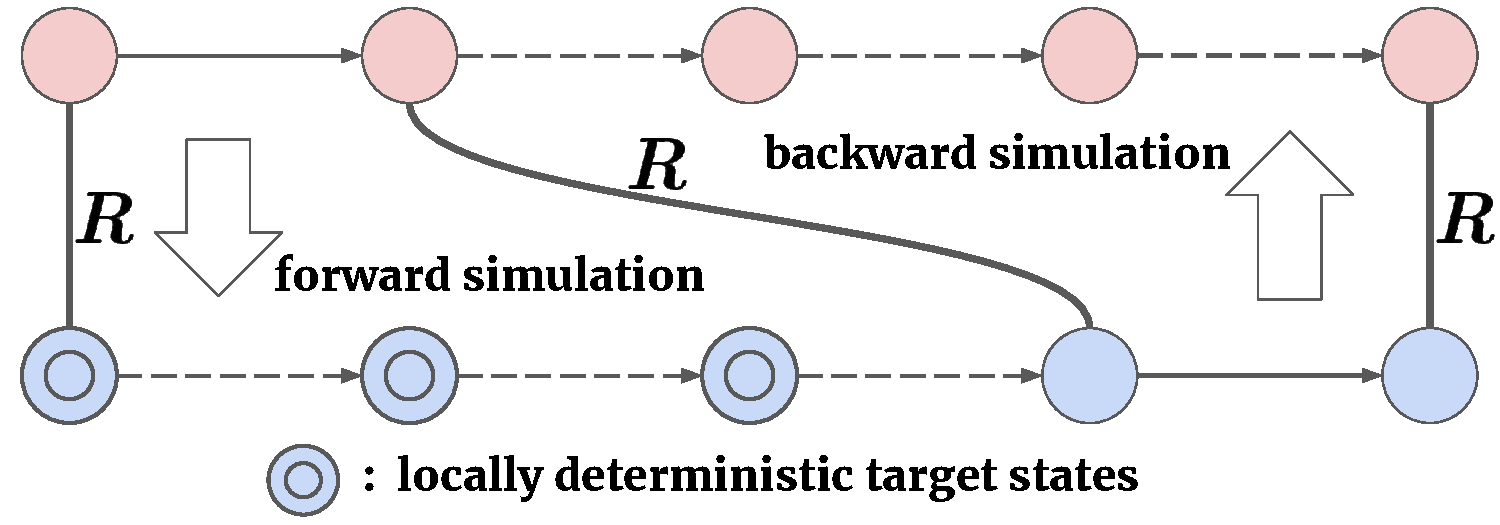
\includegraphics[width=0.7\textwidth]{images/mixed-sim-bold.pdf}
%% 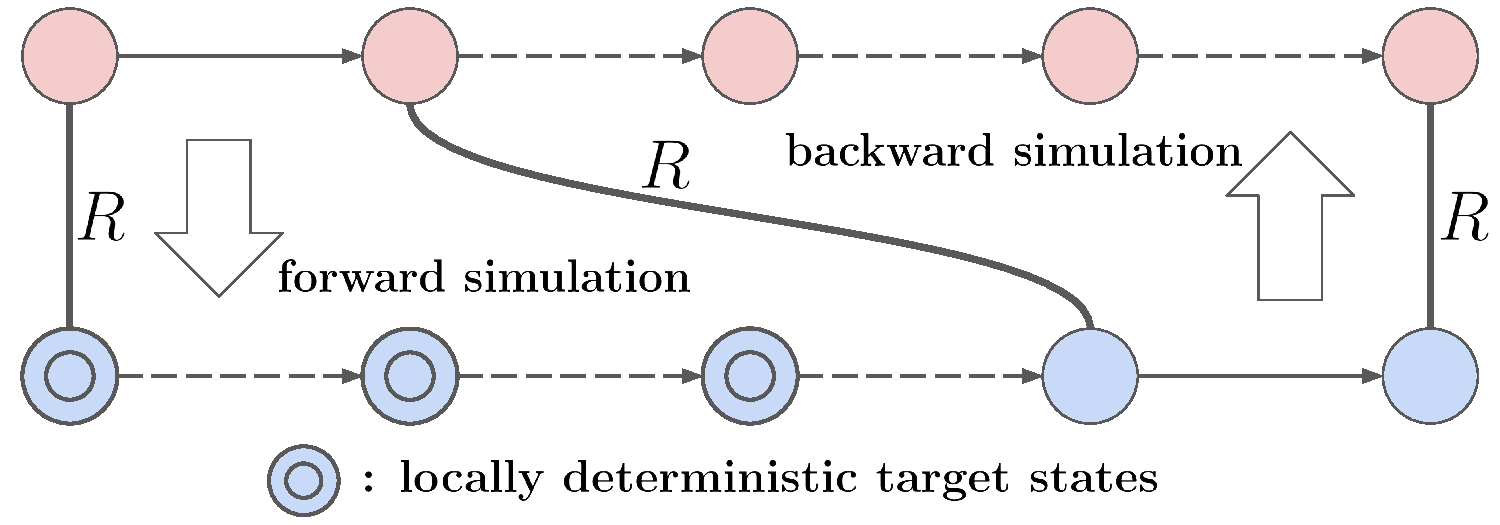
\includegraphics[width=0.7\textwidth]{images/mixed-sim.pdf}
\caption{A visualized example of mixed simulations}
\label{fig:mixedsim}
\end{figure}

\section{CompCertM}
\label{sec:compiler:compcertm}

Based on the theories we presented so far, we develop \ccm{}, an extension of \cc{} with the
repaired interaction semantics and open simulations to support multi-language linking.  We state
\ccm{}'s compositional correctness results (\Cref{sec:results:compiler}) and evaluate its
verification efforts (\Cref{sec:results:evaluation}).  \ccm{} currently supports the x86 backend only.
We do not currently see any technical problem with supporting other architectures.

\subsection{Compositional Correctness}
\label{sec:results:compiler}

\ccm{} uses open simulations with three parameters:
memory relations, symbol relations and memory predicates
(see \Cref{sec:main-verification:opensim} for details).
It supports $(i)$ the memory relations discussed in \Cref{sec:overview-verification:injection}:
identity, extension and (enriched) injections with no or any given module-local invariant;
$(ii)$ two symbol relations: one for keeping identical symbols in the source and target
and the other for allowing elimination of global variables in the target (only allowed for memory injections), needed for \code{Unusedglob} and \code{Unreadglob};
$(iii)$ two memory predicates: one for no analysis and the other for the value analysis of \cc{}.

Let $\rels$ be the set of open simulations with all possible parameters.
To apply RUSC, we prove that the \ccm{} compiler $\mathcal{C}$ transforms the source module with
a series of passes that are independently verified using open simulations in $\rels$.
\begin{lemma}[Pass Correctness]\label{thm:results-passes}
  For any \textrm{Clight} module $S$ and \textrm{Asm} module $T$, if $\mathcal{C}(S) = T$, then
  there exist intermediate modules $M_0, M_1, \cdots, M_n$ such that:
  \begin{enumerate}
  \item $M_0 = S$ and $M_n = T$; and
  \item $\forall i \in [0,n),~ \exists R \in \rels,~ (M_i, M_{i+1}) \in R$~.
  \end{enumerate}
\end{lemma}

We also prove all \textrm{Clight} and \textrm{Asm} modules are self-related.
\begin{lemma}[Self-Relatedness]\label{thm:results-relatedness} For any \textrm{Clight} or \textrm{Asm}
  module $M$, we have $M \in \self{\rels}$.
\end{lemma}
\noindent
\revision{Note that
  since we define illegal interference from Asm
  (\ie causing different behaviors in the source and target) as undefined behaviors (UBs)
  as shown in \Cref{sec:compiler:solution},
  every Asm module can be self-related.}

From \Cref{thm:results-passes,thm:results-relatedness}, the RUSC relation for the compiler follows.
\begin{theorem} [Modular Correctness]\label{thm:results-modular}
  For any \textrm{Clight} module $S$ and \textrm{Asm} module $T$, if $\mathcal{C}(S) = T$:
  \[
    {S} \rusc_\rels {T} \quad\text{with}\quad S,T \in \self{\rels}~.
  \]
\end{theorem}

\noindent
This theorem provides a truly compositional correctness
thanks to the compositionality of RUSC (\Cref{thm:rusc}):
%% The fact that the source and target are related by RUSC
%% implies that they satisfy behavioral refinement by adequacy of RUSC, and moreover
the relation can be freely (\ie vertically or horizontally) composed with any verification using RUSC
including that against mathematical specifications.
As an example, the following compositional correctness follows.
\begin{corollary} [Compositional Correctness 1]\label{thm:results-compiler}
  Let $(S_1,T_1), \ldots, (S_n,T_n)$ be pairs of source and target modules.
  If each pair is either compiled (\ie $\mathcal{C}(S_i) = T_i$ with $S_i$ \textrm{Clight} and $T_i$ \textrm{Asm}), or a self-related context (\ie $S_i = T_i \in \self{\rels}$), then
  \[
    \beh{S_1 \llink \cdots \llink S_n} \supseteq \beh{T_1 \llink \cdots \llink T_n}~.
  \]
\end{corollary}
%
\noindent This correctness theorem is compositional in the sense that behavior is refined in the
presence of any self-related contexts such as arbitrary \textrm{Clight} and \textrm{Asm} modules
(\Cref{thm:results-relatedness}).





Note that \textrm{Clight}, not \textrm{\cc{} C}, is the source language in the above theorems.  One of the
reasons is that \textrm{Clight} is the source language for most verification frameworks based on
\cc{}, such as VST~\cite{VST}, \ccc{}, and \ccx{}.  More importantly, we found that
\textrm{\cc{} C} is incompatible with memory injections.  Specifically,
\textrm{\cc{} C} imposes a strict alignment requirement on memory blocks of size zero, which, however,
%% but the requirement
is not preserved by memory injections.
%% For this reason, we cannot achieve full horizontal compositionality
%% in the presence of both \textrm{\cc{} C} modules and compiler passes verified using memory injections.
In other words, \textrm{\cc{} C} modules are not always self-related by memory injections.\footnote{This problem
  would be solved if one strengthens memory injections with more strict alignment requirements.}

\myparagraph{Supporting \textrm{\cc{} C}}
However, we can still prove a compositional correctness (not modular correctness as in \Cref{thm:results-modular}) for \textrm{\cc{} C}
following \scc{}'s \emph{Level A} technique~\cite{kang:scc},
which exploits the fact that all \textrm{CompCert C} modules are transformed to \textrm{Clight} modules
by the same two passes.
Specifically, the first pass is verified using an open simulation with the memory identity
and the second pass with memory injections, as done in the original \cc{}.
Then the following lemma follows from horizontal compositionality and adequacy of
open simulations (with memory identity and injection) and transitivity of behavioral refinement.

\begin{lemma} [ClightGen Correctness]\label{thm:results-clightgen}
  Let $(S_1,T_1), \ldots, (S_n,T_n)$ be pairs of source and target modules.
  If each pair is either translated (\ie $\textrm{ClightGen}(S_i) = T_i$ with $S_i$ \textrm{\cc{} C} and $T_i$ \textrm{Clight}), or a self-related context (\ie $S_i = T_i \in \self{\rels}$), then
  \[
    \beh{S_1 \llink \cdots \llink S_n} \supseteq \beh{T_1 \llink \cdots \llink T_n}~.
  \]
\end{lemma}



By composing \Cref{thm:results-compiler}, \Cref{thm:results-clightgen} and \Cref{thm:results-relatedness}, we have the following theorem.
\begin{theorem} [Compositional Correctness 2]\label{thm:results-compiler2}
  Let $(S_1,T_1), \ldots, (S_n,T_n)$ be pairs of source and target modules.
  If each pair is either compiled (\ie $\mathcal{C}(S_i) = T_i$ with $S_i$ \textrm{\cc{} C} or \textrm{Clight} and $T_i$ \textrm{Asm}), or a self-related context (\ie $S_i = T_i \in \self{\rels}$), then
  \[
    \beh{S_1 \llink \cdots \llink S_n} \supseteq \beh{T_1 \llink \cdots \llink T_n}~.
  \]
\end{theorem}


\myparagraph{Adequacy w.r.t. Physical Semantics}


We show that the repaired interaction semantics is adequate w.r.t. the physical semantics of \cc{},
where the former uses the language-independent linking $\llink$ and the latter the syntactic linking $\plink$
concatenating modules of the same language.

We prove that the physical semantics refines the repaired interaction semantics for \textrm{Asm} modules
using a closed simulation of \cc{} with memory injections.
\begin{theorem}[Adequacy w.r.t. Assembly]\label{thm:results-adequacy-asm}
  Let $M_1, \cdots, M_n$ be \textrm{Asm} modules.  We have:
  \[   \beh{M_1 \llink \ldots \llink M_n} \supseteq  \beh{M_1 \plink \ldots \plink M_n} ~.\]
\end{theorem}
\noindent
\revision{This theorem allows us to carry verification results on the interaction semantics such as \Cref{thm:results-compiler2}
down to \cc{}'s Asm semantics with syntactic linking.}



Conversely, we prove that the repaired interaction semantics refines the physical semantics for \textrm{\cc{} C} modules
using a closed simulation of \cc{} with memory identity.
This result is useful because we want to allow separate compilation (of C modules) on the compiler side, and on the program verification side, we want to hide complexities from inter-module steps.
\begin{theorem}[Adequacy w.r.t C]\label{thm:results-adequacy-c}
  Let $M_1, \cdots, M_n$ be \textrm{\cc{} C} modules.  We have:
  \[  \beh{M_1 \plink \ldots \plink M_n} \supseteq \beh{M_1 \llink \ldots \llink M_n}  ~.\]
\end{theorem}


In some sense, the \Cref{thm:results-compiler2,thm:results-adequacy-asm,thm:results-adequacy-c} together forms a strong stress-test for a language-independent linking, and our results show strong evidence that our repaired interaction semantics is indeed adequate (in a literal sense).
Specifically, if one of the three desiderata is missing, it is trivial to find language-independent linking satisfying the others.
Without \Cref{thm:results-adequacy-asm}, one can define interaction semantics to always execute UB; then, the other theorems become trivial.
Without \Cref{thm:results-adequacy-c}, one can define the behavior of interaction semantics to an empty set.
Without \Cref{thm:results-compiler2}, one can define $\llink \defeq \plink$.

%% These results mean that the repaired interaction semantics does not give too few behaviors to assembly programs (e.g., missing physically observable behaviors), nor does it give too many behaviors to well-typed C programs (e.g., giving UB to them).


Interestingly, by composing \Cref{thm:results-compiler2,thm:results-adequacy-asm,thm:results-adequacy-c}, we obtain
the same separate compilation correctness result of \scc{}~\cite{kang:scc}:

\begin{corollary}[Separate Compilation Correctness]
  Let $S_1, \ldots, S_n$ be \textrm{\cc{} C} modules and $T_1, \ldots, T_n$ be \textrm{Asm} modules.
  If $\mathcal{C}(S_i) = T_i$ for each $i$, we have:
  \[
    \beh{S_1 \plink \cdots \plink S_n} \supseteq \beh{T_1 \plink \cdots \plink T_n}~.
  \]
\end{corollary}

\youngju{Just mention that \ccc{} does not satisfy upperbound, and explain it in appendix?}
\youngju{here? or appendix?: To this end, we have strengthened \cc{}'s type checker in a number of
  ways, ruling out trivially wrong (according to C standard) programs more than before.  We rule out
  (i) a program that contains an identifier that is not declared in the module (ii) ``return''
  (without value) statement used for non-void function (iii) ``return'' (with value) statement used
  for void function (iv) function arguments containing void type.  (v) has duplicate (function or
  global variable) identifiers (vi) A function argument with size bigger than INT\_MAX (\cc{}
  already aborts on such programs)}





\subsection{Evaluation of Verification Efforts}\label{sec:results:evaluation}

\begin{table}[t]
\footnotesize

\parbox{\linewidth}{
\caption{SLOC of \ccm{} and related works --- compared to its baseline \cc{}, respectively}
\begin{tabu}{@{}l@{\hspace{1.55pt}}|[1.25pt]@{\hspace{1.55pt}} c @{\hspace{1.55pt}}|@{\hspace{1.55pt}} c @{\hspace{1.55pt}}|@{\hspace{1.55pt}} c @{\hspace{1.55pt}}|[1.25pt]@{\hspace{1.55pt}} c @{\hspace{1.55pt}}|@{\hspace{1.55pt}} c @{\hspace{1.55pt}}|[1.25pt]@{\hspace{1.55pt}}}
Portion     & \shortstack{\cc{} \\ 3.5} & \ccr{} 3.5        & \ccm{} pack                                               & \shortstack{\cc{}\\ 2.1} & \ccc{} \\
\hline
Pass Proofs & 34,376    & 35,893 (+4.41\%)  & \newrevision{4,923(+14.32\%)}                                          & 21,215    & 52,140 (+145.77\%) \\
The Rest    & 85,617    & 87,965 (+2.74\%)  & \newrevision{25,558(+29.85\%)}  & 59,365    & 107,910 \hspace{.6mm} (+81.77\%) \\
Total       & 119,993   & 123,858 (+3.22\%) & \newrevision{30,481(+25.40\%)}                                         & 80,580    & 160,050 \hspace{.6mm} (+98.62\%) \\
\end{tabu}
\\
\begin{tabu}{@{}l@{\hspace{1.55pt}}|[1.25pt]@{\hspace{1.55pt}} c @{\hspace{1.55pt}}|@{\hspace{1.55pt}} c @{\hspace{1.55pt}}|[1.25pt]@{\hspace{1.55pt}}}
Portion     & \shortstack{\cc{} \\ 3.0} & \ccx{}             \\
\hline
Pass Proofs & 26,466    & 30,572 (+15.51\%)  \\
The Rest    & 82,312    & 121,532 (+47.65\%) \\
Total       & 108,778   & 152,104 (+39.83\%) \\
\end{tabu}
\label{table:evaluation-ours}
}

%% \parbox{\linewidth}{
%% \label{table:evaluation-ours}
%% }
    
\parbox{0.38\linewidth}{
\vspace{4mm}
\caption{\mbox{Breakdown of \ccm{} pack}}
\begin{tabu}{@{}l | l@{}}
Portion                          & SLOC                                                                                                     \\
\hline
\revision{Proofs about Intermodule Steps} & \newrevision{4,923}                                                                                                    \\
Interaction Semantics/Properties & 1,940                                                                                                    \\
Language Semantics/Properties    & 1,701                                                                                                    \\
Self Simulations                 & \newrevision{5,593}                                                                                                    \\
\cc{}  Metatheory Extension      & \newrevision{4,688}                                                                                                    \\
\ccm{} Metatheory                & \newrevision{7,656}                                                                                                    \\
Mixed Simulation                 & 1,090                                                                                                    \\
Adequacy w.r.t. Asm              & 2,890                                                                                                    \\
\end{tabu}
\label{table:evaluation-breakdown}
}
\hfill
\parbox{0.45\linewidth}{
\vspace{4mm}
\caption{SLOC of additional developments}
%% \begin{tabu}{@{}l @{\;} |[1.25pt] @{\;} r @{\;} | @{\;} r @{\;} | @{\;} r @{\;} | @{\;} r @{\;} | @{\;} r @{}}
%% Portion                          & \shortstack{\texttt{Unreadglob} \\ 3.5} & \shortstack{\texttt{Unreadglob} \\ pack} & \texttt{mutual-sum} & \texttt{utod} & \shortstack{Adequacy \\ w.r.t. C} \\
%% \hline
%% Pass Proofs                      & 1,842                   & 338                      & 3,088               & 361           & -             \\
%% The Rest                         & 260                     & 1,933                    & 2,707               & 424           & 4,044         \\
%% Total                            & 2,102                   & 2,271                    & 5,795               & 785           & 4,044         \\
%% \end{tabu}
\begin{tabu}{@{}l @{\;} |[1.25pt] @{\;} r @{\;} | @{\;} r @{\;} | @{\;} r @{\;} | @{\;} r @{\;} | @{\;} r @{}}
Portion                          & \shortstack{\texttt{Unreadglob} \\ 3.5} & \shortstack{\texttt{Unreadglob} \\ pack} & \shortstack{Adequacy \\ w.r.t. C} \\
\hline
Pass Proofs                      & 1,842                   & 338                      & -             \\
The Rest                         & 260                     & 1,933                    & 4,044         \\
Total                            & 2,102                   & 2,271                    & 4,044         \\
\end{tabu}
\label{table:evaluation-others}
}%
\end{table}

\youngju{There are two ``unreadglob'' columns, one for \cc{} and one for pack. Simplify it}
\youngju{How about reducing caption text size?}
\jeehoon{``Per-pass'', ``Metatheory'', and ``Total'' instead of ``Pass Proofs'', ``The Rest'', and ``Whole''}

To demonstrate that \ccm{} is lightweight,
we compare significant lines of code (SLOC) of \ccm{}, \ccc{}, and \ccx{} with
those of their baseline \cc{} versions 3.5, 2.1, and 3.0, respectively.
Overall, \ccm{} adds less code to \cc{} than \ccc{} and \ccx{} do,
and in particular significantly less code than \ccc{} for the proofs of compiler passes.%
\footnote{\revision{Note that \ccc{} allows horizontal compositionality between any intermediate languages (ILs)
  while \ccm{} only between Clight and Asm since self-relatedness is proven only for the two.
  Though practically unnecessary, supporting linking between arbitrary ILs in \ccm{} would increase SLOC to prove self-relatedness for the other ILs.}}
\newrevision{Also note that \ccr{} uses the enriched memory injections of \Cref{sec:overview-verification:injection:dynamic} instead of the original memory injections
in order to give reusable main lemmas for both closed and open simulations.
Since \ccr{}'s pass proofs are only 4.41\% larger than \cc{}'s, 
the overhead due to handling the private memory components of enriched memory injections is, roughly speaking, at most 4.41\%.}

\Cref{table:evaluation-ours} summarizes the comparison.
For each compiler (\ie each column),
the rows report SLOC for the proofs of all compiler passes (Pass Proofs),
the rest of the development (The Rest),
and their summation (Total).
Note that \ccm{} is split into \ccr{} and \ccm{} pack, for which the former is our refactoring
of \cc{} and the latter is an additional package to support multi-language linking.
We counted SLOC reported by
\code{coqwc}.\footnote{Concretely, we counted ``spec'' and ``proof'' lines reported by \code{coqwc}.
  Because we use a different criteria for line numbers, they are different from those reported in
  prior work~\cite{stewart:ccc,gu:dscal,wang:saccx}.}  When counting SLOC, we excluded the following
code for fair comparison: $(i)$ code for other architectures than x86 because all three projects support
only x86; $(ii)$ code for the parser and type checker introduced in later versions of \cc{}; and $(iii)$ code for \textrm{ClightGen}, which is not supported by both \ccx{} and
\ccc{}.  We also excluded \ccc{}'s legacy proofs for the original compiler correctness.  We used the
latest development branches for the three projects.\footnote{Development as of November 8, 2019, available at: \url{https://github.com/snu-sf/compcertr}, \url{https://github.com/snu-sf/compcertm}, \url{https://github.com/PrincetonUniversity/compcomp}, \url{https://github.com/DeepSpec/dsss17/tree/master/CAL}}








\Cref{table:evaluation-breakdown} analyzes the \newrevision{30,481} SLOC for \ccm{} pack.
\revision{The pass proofs consist of \newrevision{4,923} SLOC for reasoning about intermodule steps, which is
  sometimes nontrivial since they perform the logical instrumentation presented in \Cref{sec:compiler:solution}.
  Note that \ccr{} provides proofs for intramodule steps as main lemmas, which are reused in \ccm{}.
}
The rest consists of
1,940 SLOC for the repaired interaction semantics and its properties;
1,701 SLOC for properties of each language such as determinism and receptiveness;
5,576 SLOC for self-relatedness (\Cref{thm:results-relatedness});
4,687 SLOC for extending the metatheory of CompCert;
7,569 SLOC for open simulations and other metatheory for \ccm{};
1,090 SLOC for mixed simulation; and
2,890 SLOC for adequacy w.r.t. assembly (\Cref{thm:results-adequacy-asm}).

%% \Cref{table:evaluation-others} shows SLOC for the new optimization pass and the verification examples
%% given in the dissertation.  Note that \code{Unreadglob} 3.5 adds the optimization to \ccr{} proving closed simulation
%% and \code{Unreadglob} pack to \ccm{} proving open simulation, which reuses the proof of \code{Unreadglob} 3.5 for intramodule steps.
%% As the verification of \code{mutual-sum} and \code{utod} show, directly proving
%% open simulation between programs and specifications is costly. 
%% We believe that program logics like VST~\cite{VST} can be used to prove such simulation,
%% which could significantly reduce the verification cost.
\Cref{table:evaluation-others} shows SLOC for the new optimization pass.  Note that \code{Unreadglob} 3.5 adds the optimization to \ccr{} proving closed simulation
and \code{Unreadglob} pack to \ccm{} proving open simulation, which reuses the proof of \code{Unreadglob} 3.5 for intramodule steps.


\section{Formal Semantics}
\label{sec:compiler:semantics}
abc

\section{Formalization of Verification Techniques}
\label{sec:compiler:verification}
abc

\section{Related Work}
\label{sec:compiler:related}
abc

%% \input{unsoundall}
Compiler rightfully assumes two properties about its context (\ie{} assemblies that could be linked with) and exploit it in its translation.
First, compiler assumes \textit{callee-save registers} to remain the same across a function call.
This property is vital for compiler performance, because without this assumption a compiler should always spill its data into memory whenever it encounters a call to external function.
Second, compiler assumes a variable that is not leaked, \ie{} \textit{private}, to be unchanged across during a function call.
A simple example showing the how compiler uses this assumption is \Cref{fig:compiler}.
Constant propagation, one of the most important optimization, translates (a) into (b) assuming *x it is not changed.

However, an arbitrary assembly may break these properties.
First property could easily be broken if \code{g} writes to a callee-save register without recovering it.
Suppose (a) is compiled to an assembly where \code{x} is stored in a callee-save register, say \code{\%rbx}.
If it is linked with (c), \code{f} will return 1.
Second property could also be broken and one possible reason is illegal access to the data passed in callee-save register. %% another reason: guessing. idsim prevents it
Similarly, if \Cref{fig:unsoundall}-(a) linked with (b) it will return 1.

This is an essential problem when defining a general multi-language semantics, regardless of how we define semantics.
We stress \textit{general} here to note that previous works such as \scc{} and \ccx{} were free from this problem.
This is because they were interested only in a restricted set of well-formed assemblies (compiler-generated assemblies and assemblies proven to satisfy so called \textit{primitive specification}, respectively).

In order to define a sound semantics, we should give \textit{undefined behavior} to such ill-behaved assembly, precisely.
Undefined behavior can be understood as a tool to exclude ill-behaved program from reasoning in a \textit{semantic} way.
Mathematically, undefined behavior is a set of all behaviors.
\todo{explain it - enables refinement, disables verification}


%% Mathematically, undefined behavior is a set of all behaviors.
%% By giving undefined behavior to an ill-behaved program, we can attain \textit{soundness} of our semantics: \ie{} the semantics validates compiler optimizations and actual behavior refines behavior given by the semantics.

%% We want our semantics to support general.
%% Instead of syntactically quantifying, semantically quantifying precisely. ---> difference between CCX?

\myparagraph{Semantics (tentative)}
Similar to \ccc{}, we build multi-language semantics by instantiating interaction semantics but with substantially different ingredients.
Before we proceed, we will briefly explain interaction semantics.

Intuitively, the idea behind interaction semantics is to model multi-language semantics by gluing together each languages’ existing semantics, while considering them as a black box.
To this end, whenever a function of a language, say, $L$ is called, a state of type $L.(state)$ is spawned and dedicated.
As a consequence, the behavior of that function can be described solely by reusing $L$'s semantics, considering only its dedicated state and ignoring an outside world.

A problem with \ccc{} was that it was unsound, as the first property was not enforced.
As mentioned above, the actual behavior of \Cref{fig:unsoundall} is returning 1, as there is one, shared register set.
However, in interaction semantics, each function has its own state, (register set, here).
As a consequence, b.s modifies \textit{its} \code{\%rbx} and it does not affect that of a.s.
Therefore, \ccc{}'s semantics will confidently say that it returns 0.

In order to address this discrepancy, it is crucial to enforce the calling convention somehow.
In other words, if some callee-save register has a different value between the beginning and the end of a function, it should be \textit{undefined behavior}.
This discovery leads us to the next question: what should be the initial value of such a callee-save register?
In \ccc{}, it is an undef value.
This is an appropriate choice because its actual value on runtime could differ arbitrarily by its caller.
%% Why not zero?
However, adding one to undef value still results in undef value.
Therefore, it does not trigger undefined behavior and the problem is unresolved.
Note that whatever value you chose (\eg{} 0) to initialize \code{\%ebx}, I can modify \code{\%rbx + 1} into the value of your choice, and the problem remains the same.

One naive fix is to initialize it dynamically with the value of the caller's register, instead of a statically fixed one, but it still does not work.
In that case, examples above will properly give undefined behavior.
However, recall that we are defining a multi-language semantics: what if the caller is a C function?
We cannot foresee what caller's register's value will be, as we do not know how the caller will be compiled: the semantics should be sound no matter which compiler and optimizations we use.

%% We argue that the flaw of this game lies in \textit{determinism}.
We argue that the root cause of this problem is \textit{determinism}.
Our solution is to initialize each register with an arbitrary value, in a \textit{nondeterministic} way.
By doing so, if there is a single choice of value that causes callee-save checking to fail, it is undefined behavior.
That is, we are effectively enforcing calling convention to be satisfied \textit{no matter what values} are passed in callee-save registers.

However, full nondeterminism breaks the second property.
\todo{}



\myparagraph{Proof (tentative)}
\todo{mixed simulation}



-----------------------------------------------------------------
-----------------------------------------------------------------
-----------------------------------------------------------------
-----------------------------------------------------------------
-----------------------------------------------------------------
-----------------------------------------------------------------
-----------------------------------------------------------------
-----------------------------------------------------------------
-----------------------------------------------------------------
-----------------------------------------------------------------
-----------------------------------------------------------------

Consider the following example: \Cref{fig:compiler}-(c).
Here, \code{y} is introduced just to forbid constant propagation.
In its final target, \code{y} will be stored in a callee-save register and
\Eg{} a compiler will translate \Cref{fig:compiler} a compiler will assign a callee-save register for the variable \code{x}, and


and a sound semantics should give undefined behavior on such assembly.
Basically, Callee-save registers


This is an unavoidable



Similar to \ccc{}, we build multi-language semantics by instantiating interaction semantics, but with substantially different ingredients.

Compiler rightfully assumes callee-save registers remain the same across a function call, but arbitrary assembly code may break this property.
- this is an essential challenge
- in \scc{}, there was no problem

In \ccc{}, defined it with undef, but it is not sound


The last

\myparagraph{Interaction Semantics}

\myparagraph{Memory (tentative)}



%% introduced and then by will describe why \ccc{}'s semantics fails to satisfy desiderata, and lead you to our solution step by step.
%% Similar to \ccc{}, we build multi-language semantics by instantiating interaction semantics, but with substantially different ingredients.

Similar to \ccc{}, we build multi-language semantics by instantiating interaction semantics, but with substantially different ingredients.
\myparagraph{Interaction Semantics}
Intuitively, the idea behind interaction semantics is to model multi-language semantics by gluing together each languages’ existing semantics, while considering them as a black box.
To this end, whenever a function of a language, say, $L$ is called, a state of type $L.(state)$ is spawned and dedicated.
As a consequence, the behavior of that function can be described solely by reusing $L$'s semantics, considering only its dedicated state and ignoring an outside world.

%% \input{unsoundall}
\myparagraph{Callee-save Checking}











\ccc{}'s semantics is unsound as it is not \lbound{}, and the key ingredient to address this problem is nondeterminism.

%% Consider this example \Cref{fig:unsoundall}.
\Cref{fig:unsoundall} shows why \ccc{} is not \lbound{}.
Note that these are assembly programs: we used C syntax just for readability.
When the \code{main} is linked with (a) and ran in actual CPU, it will obviously print 2.
Nonetheless, according to \ccc{}'s semantics, it prints 1!
As explained, in interaction semantics, each function call is dedicated its own state (register set, here), while in reality there is one, shared register set.
%% Take this setting for granted, caller expects its callee-save registers to remain the same across the function call.
%% \input{unsound}
The caller (main) rightfully assumes its callee-save registers to remain the same across the function call, but the callee (f) breaks the \textit{calling convention}.
In order to address this discrepancy, it is crucial to enforce the calling convention. %% on each function.
In other words, if some callee-save register has a different value between the beginning and the end of a function, it should be \textit{undefined behavior}.

This discovery leads us to the next question: what should be the initial value of such a callee-save register?
In \ccc{}, it is \textit{undef}.
This is an appropriate choice because its actual value on runtime could differ arbitrarily by its caller. %% it is impossible for callee to expect any specific value in the register. %% to know which context will call the function.
%% However, now consider the example on the right (\Cref{fig:unsound2}).
However, now suppose the \code{main} is linked with (b).
According to our slightly modified semantics (that checks if callee-save registers remain the same), \code{f} passes the checking, and it still prints 1.
Note that whatever value you chose (\eg{} 0) to initialize \code{\%ebx}, I can modify \code{INTMAX + 1} of \code{f} into the value of your choice, and the problem remains the same.

One naive fix is to initialize it dynamically with the value of the caller's register, instead of a statically fixed one, but it still does not work.
In that case, examples above will properly give undefined behavior.
However, recall that we are defining a multi-language semantics: what if the caller is a C function?
We cannot foresee what caller's register's value will be, as we do not know how the caller will be compiled: the semantics should be sound no matter which compiler and optimizations we use.

%% We argue that the flaw of this game lies in \textit{determinism}.
We argue that the root cause of this problem is \textit{determinism}.
Our solution is to initialize each register with an arbitrary value, in a \textit{nondeterministic} way.
By doing so, if there is a single choice of value that causes callee-save checking to fail, it is undefined behavior.
That is, we are effectively enforcing calling convention to be satisfied \textit{no matter what values} are passed in callee-save registers.




\myparagraph{Junk Pointers}

Nonetheless, the problem is not over yet: so far, we have only considered lower bound proof, but compiler correctness proof complicates the problem once again.
\todo{specifically, self simulation of assembly}
\todo{For efficiency ? we want our semantics to satisfy the following three constraints}.
First, \todo{initial state is injected}
\todo{explain \cc{} injection? where?}
\todo{1. it is more efficient 2. to reason arbitrary assembly. if not-injected, passing it to extcall will break reasoning}
Second, \todo{src callee-save checking succeeds -> tgt succeeds}
\todo{1. it is more efficient}
\todo{2. to reason in modular way. f := x = g(); --> src checking succeeds (U-U) tgt checking fails (0-1)}
Third, \todo{we want to allow pointer arithmetic?}

Naive nondeterminism fails to satisfy these constraints.
%% Naive nondeterminism fails.
\todo{\cc{} injection has target private pointer, the only value that injects it is undef}
\todo{src begins with undef -> second property fails}

Therefore, we developed a novel trick called \textit{junk pointer} to address this problem.
\todo{explain junk pointer and proof strategy for self sim and lower bound}





















\myparagraph{Memory}








\section{Overview}\label{sec:overview}
In this section, we show an outline of our development, key ideas of our semantics and proof technique, motivating each one by comparing with \ccc{}.

\subsection{Development Outline}\label{sec:overview:outline}
%% \todo{we will explain why our strategy is extensible in both axis}


\myparagraph{Compositional Compiler Correctness}
\ccc{}'s proof strategy is modular, but only to some extent.%% , but ours is entirely modular.
\ccc{} is modular in the sense that it proves each translation separately.
However, the simulation relation it uses is globally fixed to a \textit{single} one which is sophisticated enough to reason every pass, which currently is structured injection.
So this breaks modularity: even a trivial translation using the simplest relation is \textit{enforced} to be reimplemented to use structured injection, because of compositionality with \textit{other} translations.
Moreover, suppose that future \cc{} has introduced a translation that is too complex for structured injection to reason with.
Then, this introduction of a single pass breaks whole proof: the \textit{single} relation should be adjusted to cover it, and every existing proof should be updated accordingly.

Our proof strategy is entirely modular, and the key distinction is that we do not require vertical compositionality of \textit{simulation relation}.
\ccc{} relied on vertical compositionality of simulation relation, which is known to be a notoriously hard problem.
Not to mention its proof, a question whether such relation composes is a surprisingly nontrivial problem, and finding appropriate relation is itself an interesting research problem. \cite{TODO}
In \ccc{} context, proving vertical compositionality at least required a nontrivial amount of development: the proof is 5274 SLOC long, and it enforced to re-implement each language's semantics with effect annotations.
The problem gets more complicated if we consider multiple different relations, and we believe that is the reason why Stewart \etal{} fixed a single simulation relation. %% to avoid proving vertical compositionality as much as possible.
%% A. Ahmed, D. Dreyer, and A. Rossberg, “State-dependent representationindependence,” inPOPL, 2009
%% D. Dreyer, G. Neis, and L. Birkedal, “The impact of higher-order stateand  control  effects  on  local  relational  reasoning,”J.  Funct.  Program.,vol. 22, no. 4-5, pp. 477–528, 2012.
In contrast, as we do not require vertical compositionality of simulation relation, we are free from such problems and obtain \textit{true modularity}: each translation can choose the simulation relation of its interest.
%% Stewart \etal{} rather fixed a \textit{single, most sophisticated} simulation relation for whole translation proof.



%% \begin{wrapfigure}{R}{.4\textwidth}
\begin{figure}
  \centering
  %% 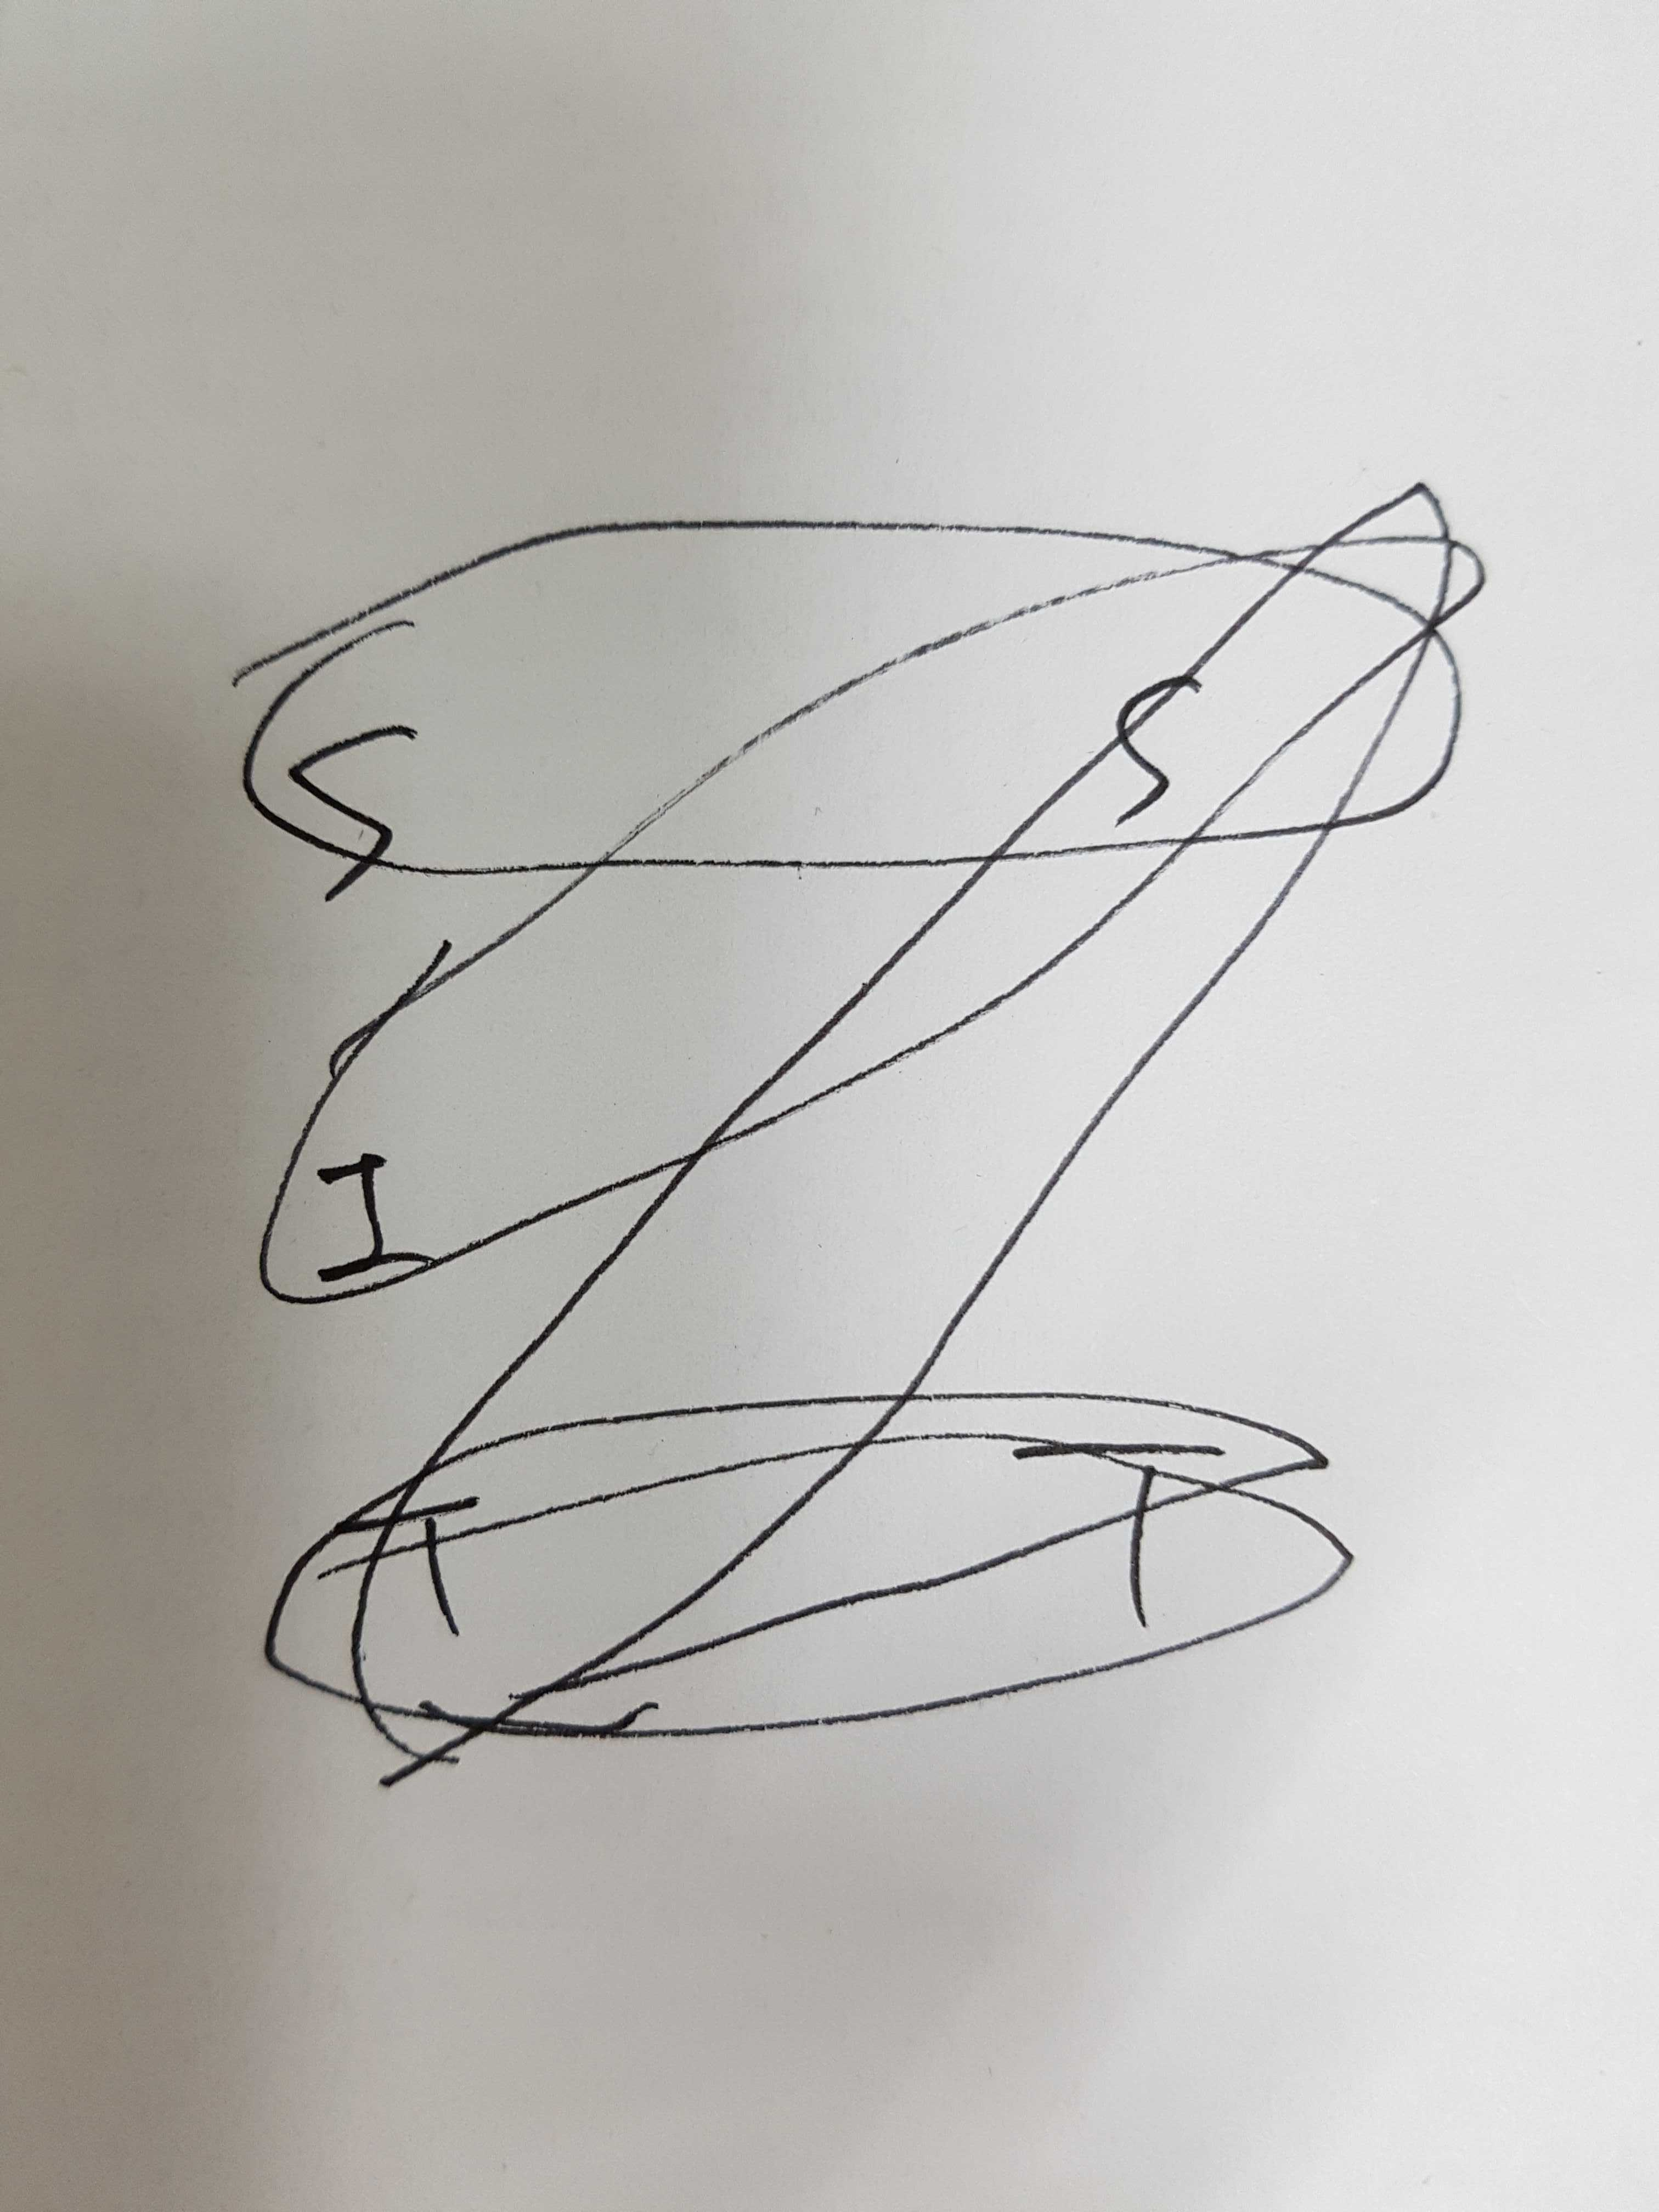
\includegraphics[width=1.0\linewidth]{images/draft-fig.jpg}
  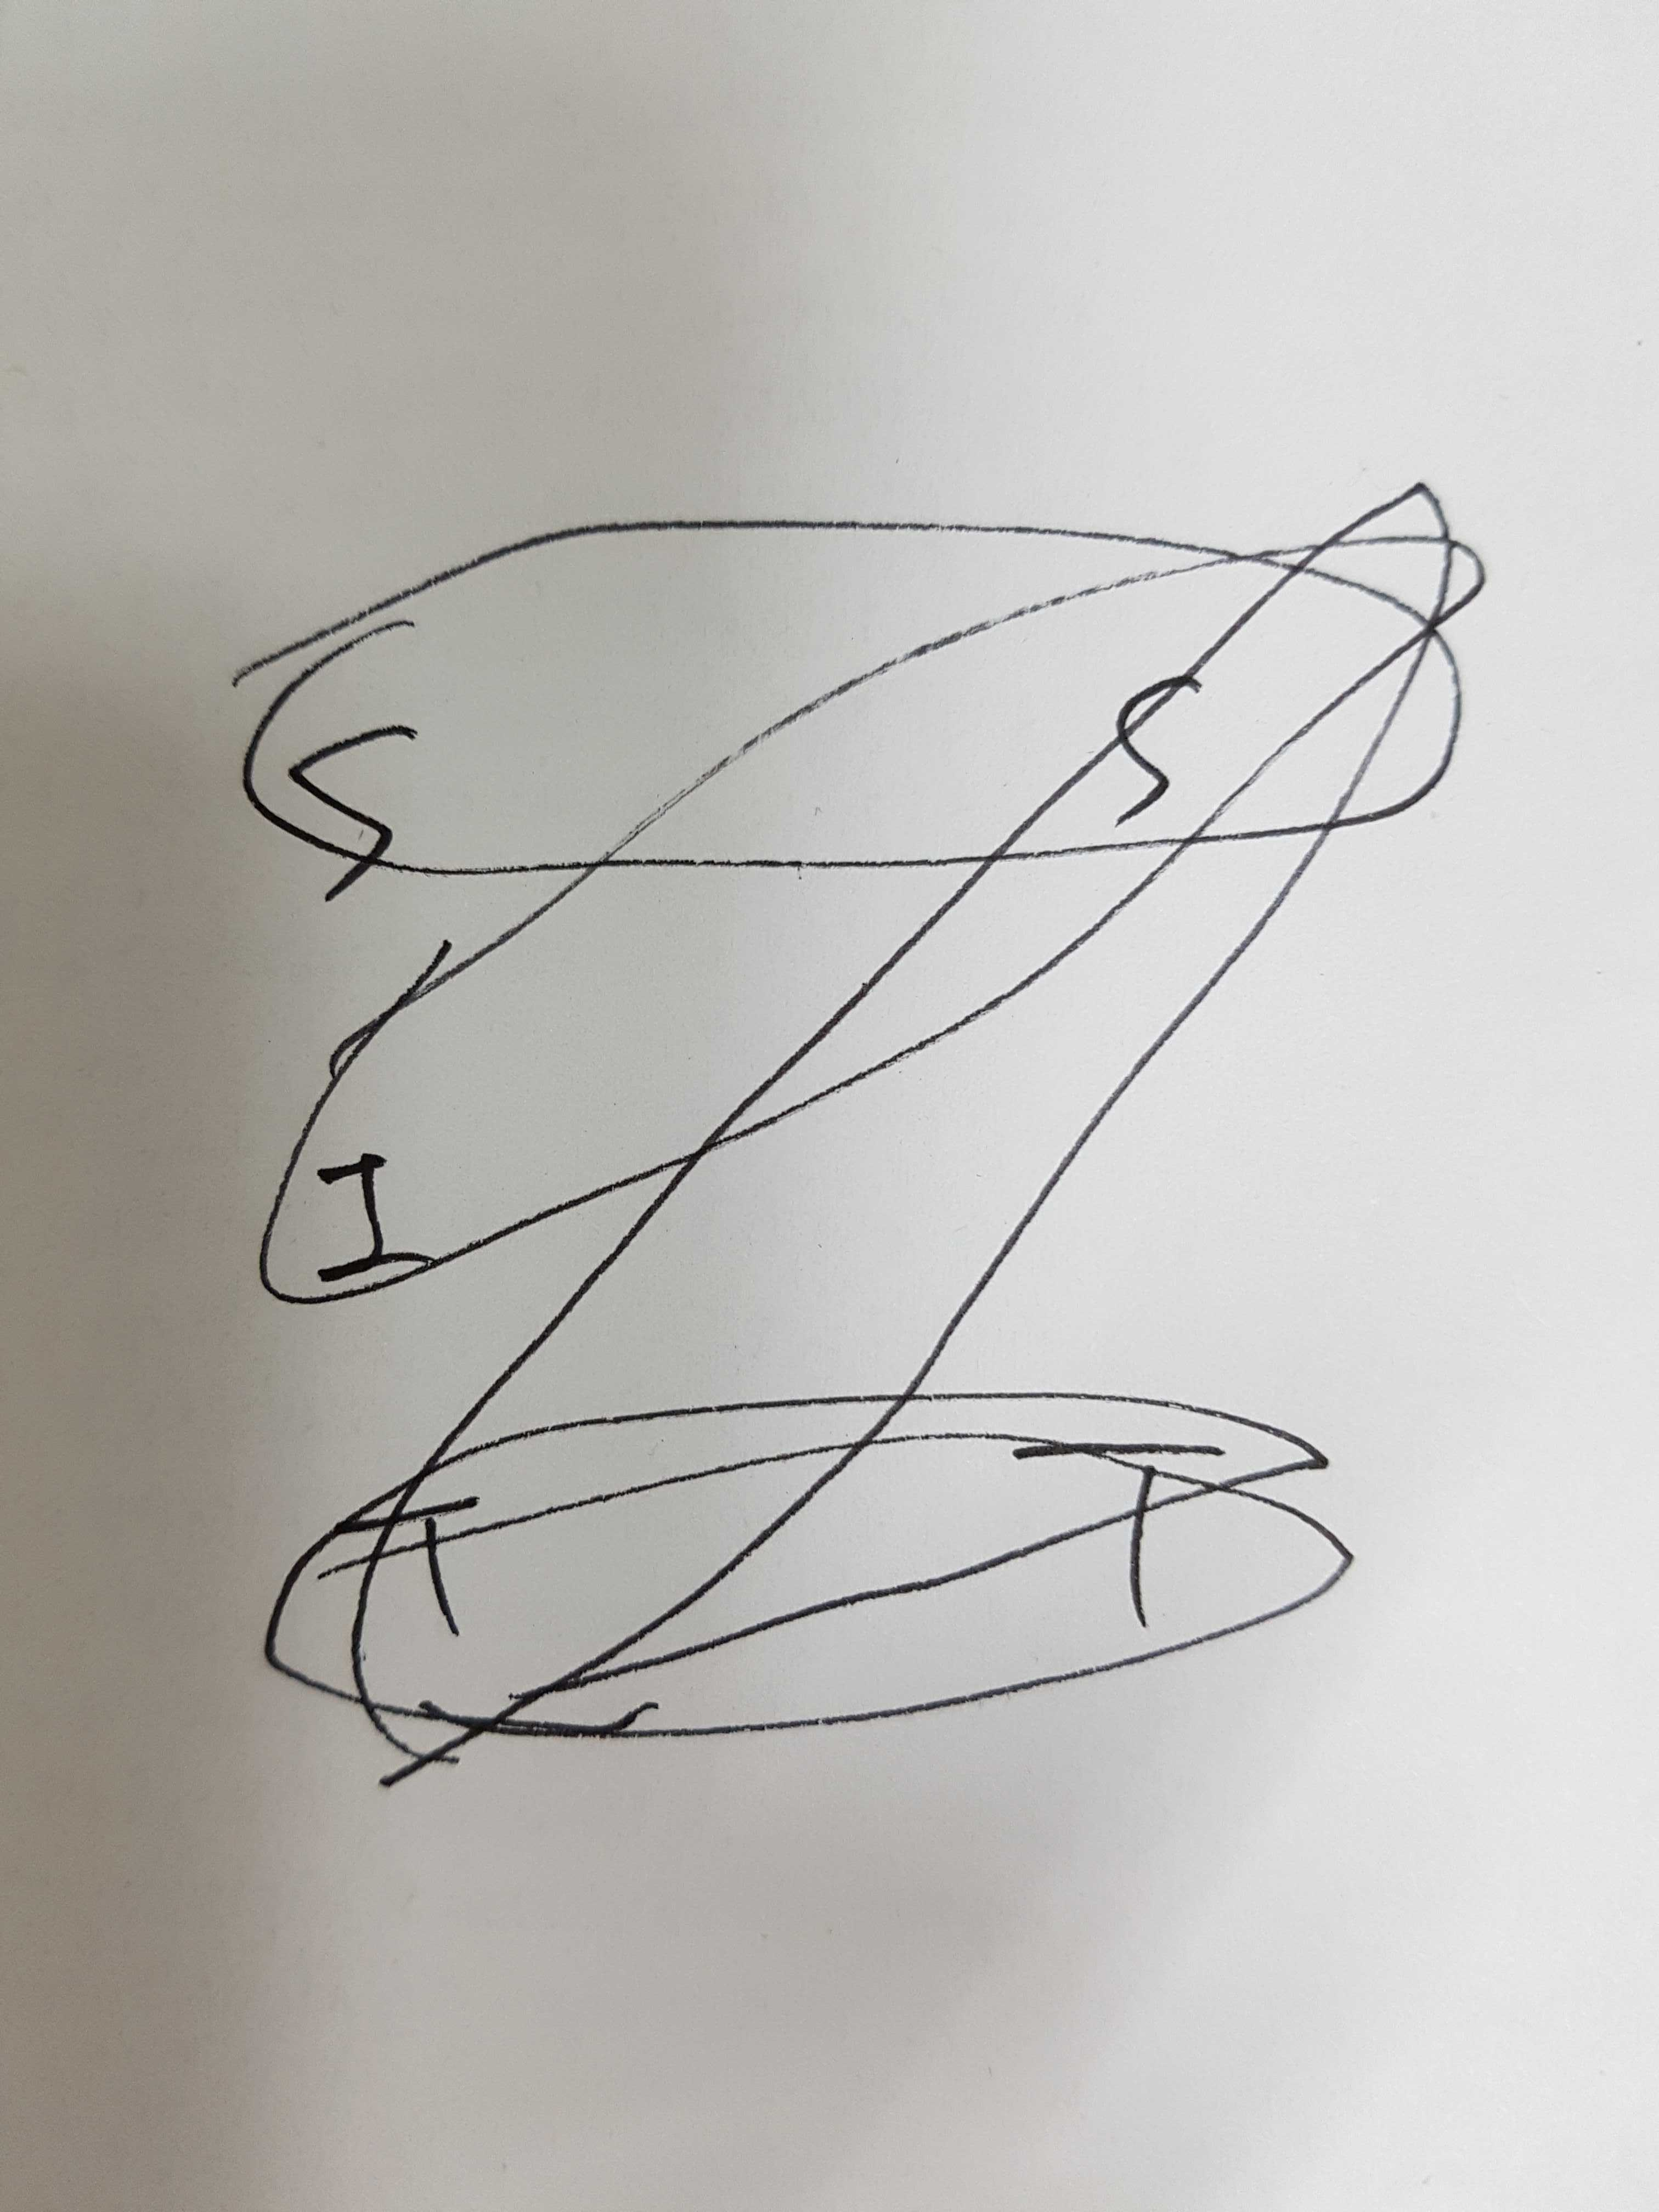
\includegraphics[width=0.35\linewidth]{images/draft-fig.jpg}
  \caption{
  }
  \label{fig:draft-fig}
\end{figure}
%% \end{wrapfigure}

We avoid proving vertical compositionality of \textit{simulation relation}, and instead, we compose in \textit{behavior} level, which is made possible because we are defining multi-language semantics.
\todo{compare with PILS - it is not multi-language semantics}
\todo{compare with Amal Ahmed? Their contextual equivalence is not modular}
%% But since all the languages in the compiler pipeline are taken into account when verifying each pass, this is far less modular than vertical compositionality.


\todo{Add simplified formalizations here? or later?}


Our proof strategy does not require such; each translation can chose whatever relation (in other words, rely and guarantee conditions) it wants.
The key distinction that leads to such difference is that we do not require vertical compositionality of \textit{simulation relation}, instead we compose in \textit{behavior} level.
Note that proving vertical compositionality is a notoriously hard work \cite{TODO}. %%pilsner?
Therefore, in order to avoid such complexity as much as possible, Stewart \etal{} rather fixed a \textit{single, most sophisticated} simulation relation for whole translation proof.

However, it is practically important to allow different simulation relation for each translation passes.
%% Note that vanilla \cc{} uses three different simulation relations, and porting it \todo{costed a lot}.
We will discuss this more in \cite{sec:overview:proof}.
Second, also, in order to prove vertical compositionality, they had to annotate each language's semantics with memory effects.


\ccc{} relies on vertical compositionality of simulation relation which harms true modularity.
In contrast, we compose in \textit{behavior} level, which is as simple as transitivity of set inclusion.

%% Like \ccc{}, we verify compiler correctness in a \textit{modular} way.
%% However, a little tweak here grants us significant benefit at the cost of proving a trivial fact.


%% but is little different, having significant benefit at the cost of proving a trivial fact.
%% Different from that of \ccc{}, our proof strategy has significant benefit at the cost of proving a trivial fact.





%% \subsection{Bounding Semantics}
\myparagraph{Lower Bound}
Lower bound is a part of soundness condition that multi-language semantics should satisfy, stating its behavior should at least contain \textit{actual behavior}.
It is formalized as follows.
%% Informally speaking, we want the behavior of multi-language semantics to at least contain an actual behavior when ran on a machine.
%% This property is a part of soundness of a semantics, and breaking it equals collapse of whole verification stack.
%% We have named this property as being \textit{bounded below} or \textit{lower bound}, and formalized it as follows.

\begin{theorem} (Lower bound)
  \[
  %% \forall \, A_{1} \, \ldots \, A_{n}, \,
  \mathcal{B}(L(A_{1}, \ldots, A_{n})) \supseteq \mathcal{B}(\llbracket A_{1} \circ \ldots \circ A_{n} \rrbracket)
  \]
\end{theorem}

\todo{explain $\circ$ notation and physical linking}

Then, together with compiler correctness proof, \todo{clarify it before} we can assure verification done in source level holds in actual behavior.
Note that we did not choose target arbitrarily: a syntactically linked assembly program is the current final target of \cc{}.
In other words, it is trusted computing base of \cc{} that syntactically linked assembly program properly models actual behavior, and we do not add any assumption.


\myparagraph{Upper Bound}
Upper bound is the dual of lower bound, and formalized as follows.
Although this property is not as vital as lower bound - it is not related to soundness - it is desirable for three reasons.
We require each C modules to be type\mymathhyphen{}checked for a technical reason which will be addressed in \Cref{sec:overview:semantics}

\begin{theorem} (Upper bound)
  \[
  %% \forall \, C_{1} \, \ldots \, C_{n}, \,
  C_{1}, \ldots, C_{n}, \, (C_{1} \circ \ldots \circ C_{n}) \; are \; type-checked \implies
  \mathcal{B}(\llbracket C_{1} \circ \ldots \circ C_{n} \rrbracket) \supseteq \mathcal{B}(L(C_{1}, \ldots, C_{n}))
  \]
\end{theorem}

First, this is a strong stress test for usability.
Note that both lower bound and compiler correctness proof becomes trivial if we define our semantics to be always undefined behavior, \ie{} set of all behaviors.
However, such semantics is not at all useful for user: one cannot verify anything with it.
Therefore, We would like to have a theorem that assures we didn't do such a thing.
Our formalization is the most sensible and strong such theorem we can think of.

Second, by composing with compiler correctness and lower bound theorem, we can get the correctness of separate compilation for free.
\todo{we support different version of \cc{}, while \scc{} cannot}
\begin{corollary} (Separate compilation correctness)
  \[                            %
  C_{1}, \ldots, C_{n}, \, (C_{1} \circ \ldots \circ C_{n}) \; are \; type\mymathhyphen{}checked \implies
  \mathcal{B}(\llbracket C_{1} \circ \ldots \circ C_{n} \rrbracket) \supseteq \mathcal{B}(\llbracket \mathcal{C}(C_{1}) \circ \ldots \circ \mathcal{C}(C_{n}) \rrbracket)
  \]
\end{corollary}
\begin{proof}
  TODO
\end{proof}
Finally, it can help reasoning and verification by hiding details of intermodule protocols.
\ie{} we want to allow users to reason about separately compiled C modules as if they were one.
%% Furthermore, with slight modification, we can get stronger theorem which allows input program to contain assembly.
To this end, instead of proving upper bound directly, we prove the following two lemmas which together imply upper bound.
Contrary to the aforementioned upper bound theorem, upper bound compression lemma can be used where source program contains assembly.

%% \todo{consequently, allow user to reason in syntactically linked program, bypassing meta-level call},
%% \todo{we assume all C modules here are type-checked for technical reason}

\begin{lemma} (Upper bound compression)
  \[
  %% \forall \, C_{1} \, C_{2} \, ctx, \,
  C_{1}, \ldots, C_{n}, \, (C_{1} \circ \ldots \circ C_{n}) \; are \; type\mymathhyphen{}checked \implies
  \mathcal{B}(L(ctx, (C_{1} \circ \ldots \circ C_{n}))) \supseteq \mathcal{B}(L(ctx, C_{1}, \ldots, C_{n}))
  \]
\end{lemma}

\begin{lemma} (Upper bound lifting)
  \[
  %% \forall \, C, \,
  C \; is \; type\mymathhyphen{}checked \implies
  \mathcal{B}(\llbracket C \rrbracket) \supseteq \mathcal{B}(L(C))
  \]
\end{lemma}





\subsection{Semantics}\label{sec:overview:semantics}
Similar to \ccc{}, we build multi-language semantics by instantiating interaction semantics, but with substantially different ingredients.
In this subsection, we will describe why \ccc{}'s semantics fails to satisfy desiderata, and lead you to our solution step by step.

\myparagraph{Interaction Semantics}
Intuitively, the idea behind interaction semantics is to model multi-language semantics by gluing together each languages’ existing semantics, while considering them as a black box.
To this end, whenever a function of a language, say, $L$ is called, a state of type $L.(state)$ is spawned and dedicated.
As a consequence, the behavior of that function can be described solely by reusing $L$'s semantics, considering only its dedicated state and ignoring an outside world.

%% However, CompComp’s semantics is unsound as it is not bounded below. Consider this example 3.
%% Note that these are assembly programs: we used C syntax just for readability. When main is linked
%% with (a) and run in actual CPU, it will obviously print 2. Nonetheless, according to CompComp’s
%% semantics, it prints 1! As explained, in interaction semantics, each function call is dedicated its
%% own state (register set, here), while in reality there is one, shared register set. The caller (main)
%% rightfully assumes its callee-save registers to remain the same across the function call, but the
%% callee (f) breaks calling convention. In order to address this discrepancy, it is crucial to enforce such
%% calling convention. In other words, if some callee-save register has different value between the
%% beginning and the end of a function, it should be undefined behavior.




\myparagraph{Nondeterminism}
%% \input{unsoundall}
\ccc{}'s semantics is unsound as it is not \lbound{}, and the key ingredient to address this problem is nondeterminism.

%% Consider this example \Cref{fig:unsoundall}.
\Cref{fig:unsoundall} shows why \ccc{} is not \lbound{}.
Note that these are assembly programs: we used C syntax just for readability.
When the \code{main} is linked with (a) and ran in actual CPU, it will obviously print 2.
Nonetheless, according to \ccc{}'s semantics, it prints 1!
As explained, in interaction semantics, each function call is dedicated its own state (register set, here), while in reality there is one, shared register set.
%% Take this setting for granted, caller expects its callee-save registers to remain the same across the function call.
%% \input{unsound}
The caller (main) rightfully assumes its callee-save registers to remain the same across the function call, but the callee (f) breaks the \textit{calling convention}.
In order to address this discrepancy, it is crucial to enforce the calling convention. %% on each function.
In other words, if some callee-save register has a different value between the beginning and the end of a function, it should be \textit{undefined behavior}.

This discovery leads us to the next question: what should be the initial value of such a callee-save register?
In \ccc{}, it is \textit{undef}.
This is an appropriate choice because its actual value on runtime could differ arbitrarily by its caller. %% it is impossible for callee to expect any specific value in the register. %% to know which context will call the function.
%% However, now consider the example on the right (\Cref{fig:unsound2}).
However, now suppose the \code{main} is linked with (b).
According to our slightly modified semantics (that checks if callee-save registers remain the same), \code{f} passes the checking, and it still prints 1.
Note that whatever value you chose (\eg{} 0) to initialize \code{\%ebx}, I can modify \code{INTMAX + 1} of \code{f} into the value of your choice, and the problem remains the same.

One naive fix is to initialize it dynamically with the value of the caller's register, instead of a statically fixed one, but it still does not work.
In that case, examples above will properly give undefined behavior.
However, recall that we are defining a multi-language semantics: what if the caller is a C function?
We cannot foresee what caller's register's value will be, as we do not know how the caller will be compiled: the semantics should be sound no matter which compiler and optimizations we use.

%% We argue that the flaw of this game lies in \textit{determinism}.
We argue that the root cause of this problem is \textit{determinism}.
Our solution is to initialize each register with an arbitrary value, in a \textit{nondeterministic} way.
By doing so, if there is a single choice of value that causes callee-save checking to fail, it is undefined behavior.
That is, we are effectively enforcing calling convention to be satisfied \textit{no matter what values} are passed in callee-save registers.




\myparagraph{Junk Pointers}

Nonetheless, the problem is not over yet: so far, we have only considered lower bound proof, but compiler correctness proof complicates the problem once again.
\todo{specifically, self simulation of assembly}
\todo{For efficiency ? we want our semantics to satisfy the following three constraints}.
First, \todo{initial state is injected}
\todo{explain \cc{} injection? where?}
\todo{1. it is more efficient 2. to reason arbitrary assembly. if not-injected, passing it to extcall will break reasoning}
Second, \todo{src callee-save checking succeeds -> tgt succeeds}
\todo{1. it is more efficient}
\todo{2. to reason in modular way. f := x = g(); --> src checking succeeds (U-U) tgt checking fails (0-1)}
Third, \todo{we want to allow pointer arithmetic?}

Naive nondeterminism fails to satisfy these constraints.
%% Naive nondeterminism fails.
\todo{\cc{} injection has target private pointer, the only value that injects it is undef}
\todo{src begins with undef -> second property fails}

Therefore, we developed a novel trick called \textit{junk pointer} to address this problem.
\todo{explain junk pointer and proof strategy for self sim and lower bound}





%\input{unsoundmem-depr}
\myparagraph{Unfreeing Memory}

\ccc{} is not \lbound{}, for another reason, and we address this by introducing a new memory operation, \textit{unfree}.

\todo{explain omitted detail: how memory is treated in interaction semantics}

\Cref{fig:stack-convention-depr} exposes the problem.

\todo{unlike \saccx{}, we implemented the idea inside \cc{}'s memory model}
\todo{this operation is potentially dangerous, as it might break compiler's reasoning, but we are unfreeing exactly the freed region}





\myparagraph{Typify}
\ccc{} is not \ubound{}, as passing an undefined value as an argument causes undefined behavior.

This undefined behavior is intended for compiler correctness.
\cc{} optimizations are implemented assuming that external call returns a well-typed value.
However, this notion of well-typedness is not preserved along injection (or lessdef) relation, because of undef value.
\Eg{} consider a call to external function whose return type is int.
Now, suppose the return value is undef in source and 1.0 in target.
Then, type checking succeeds in source but fails in target.
\ccc{}'s choice was to totally exclude this case, by giving undefined behavior.

Our idea is...
\todo{explain it}
\todo{1. it preserves injection (lessdef) 2. it enforces type checking}

Our idea allows upper bound theorem to hold under mild, syntactically checkable assumption, that is, passing the type checker.
In contrast, statically proving the absence of undefined value is much harder problem. \todo{is there such tool?}







\subsection{Proof}\label{sec:overview:proof}

In this section, we show the fundamental ideas of our proof technique, and explain why it allows lightweight development.

\myparagraph{Mixed simulation}
Although nondeterminism properly captures our intuition and is a key ingredient towards sound semantics, adopting this gives rise to yet another, technical but crucial problem.
For every passes (except one) \cc{} uses \fsim{}, which exploits determinism of the target language, and breaking this assumption can potentially invalidate all those existing proof.
It is even said that ``Determinism is instrumental for the simulation proofs of the compiler passes and its absence is a show stopper.'' \cite{besson:intptr}


To tame the nondeterminism introduced, we developed a proof technique called \textit{mixed simulation} which exploits \textit{local determinism}, and as a consequence, we successfully reused existing proof.
%% The idea is to exploit \textit{local determinism}.
\textit{Each step}, \xsim{} lets a user decide which simulation technique to use, either forward or backward, while forward is only allowed when the current target \textit{state} is deterministic.
To put in another way, the default option is a \bsim{}, and while vanilla \fsim{} requires determinism of the \textit{whole language} to allow forward reasoning for \textit{whole proof}, \xsim{} requires determinism of a \textit{state} and allows forward reasoning for one \textit{step}.
\nb{} except for the initial state we defined, every other state remains deterministic, and as a consequence, we can reuse existing proof at ease.
%% Therefore, we exploit these \textit{local determinism} to allow forward reasoning, and .
The idea of exploiting local determinism is formerly discovered in \cite{neis:pilsner}, but we are the first to concretize and implement the idea in the context of \cc{}. \todo{Not sure if it is really a contribution}


\myparagraph{Parameterizing memory relation}

As discussed in \Cref{sec:overview:outline}, \ccc{} enforced single memory relation (structured injection) for whole translations, and it is practically a significant problem. %% it caused a lot of extra work.
Note that \cc{} uses three different \mrel{}s so that each translation passes use the simplest but sufficient one.
The most drastic example is ``CleanupLabelsproof'', which used the simplest memory relation and was 302 SLOC.
However, after changing its memory relation into a structured injection, it is 1875 SLOC.
Specifically, the memory relation it was using is \textit{Leibniz equality}, which dramatically simplifies the proof thanks to native support from Coq.

With our proof technique, such extra work is unnecessary.
\todo{parameterized, as long as it satisfies minimal conditions and self simulation}

\myparagraph{Local preservation}
\cc{} introduced value analysis, and it introduces a new challenge.

Translation proof should only rely on it, and proof obligation is assigned to analysis.
Therefore, multiple passes use it while preservation is proven only once.

It requires rely/guarantee reasoning similarly with injection, but the passes using it is proven with extension.
It has a notion of private.

$ st\_src_{0} \sim st\_tgt_{0} \implies st\_src_{1} \sim st\_tgt{1} $

$ st\_src_{0} \sim st\_tgt_{0} \wedge sound \, st\_src_{0} \implies st\_src_{1} \sim st\_tgt{1} $

We introduce a notion of \textit{local preservation}, and obligate it to each module.
This is basically an unary version of local simulation.

One difference wit (local) simulation is that, there can be multiple analyses for single translation.
To address this, we join the private areas when it calls an external module, thereby guaranteeing every analyses' expectations.

$ st\_src_{0} \sim st\_tgt_{0} \wedge sound \, st\_src_{0} \ldots \wedge sound_{n} \, st\_src_{0} \implies st\_src_{1} \sim st\_tgt{1} $


\myparagraph{Parameterizing symbol relation}
\cc{} introduced Unusedglob pass, and it introduces a new challenge.

Global environment is constructed this way. symbols (compiletime) -> blocks (runtime).

Difference between Unusedglob and other passes - .
Question is how global definitions are injected.
So far, other optimizations did not remove or add symbols.
Therefore, the relation between source and target global environment was simple. %% equality in senv
Unusedglob breaks it - it uses more sophisticated relation between symbols.

There are different rely/guarantee here, just as memory relations.
Most of the translations expect its If this translation is using simple genv relation, than


Constructing a simulation relation that is suitable for Unusedglob break other passes.




\pagebreak
\input{outline}




\subsection{ETC}
\myparagraph{Extensibility - Unwroteglob, Removing Axiom, Dummy Stack}
\myparagraph{Removing Axiom}
.

------------------------------------------------------------------------------------------------------------------------------------------------------------





This generality was costly to achieve considering compiler verification, and Stewart \etal{} failed to reuse vanilla \cc{}: they had to decorate semantics with step relation, .
tttttttttttttttttttttttttttttttttttttttt




General is good (strongest)
General is costly to achieve - \cc{}x, structured simulation, incomplete proof, LOC, not extensible
effectful semantics
Sound
Complete proof -> VA, Unusedglob
This generality was costly to achieve, considering compiler verification, so that other approaches \cite{gu:dscal, wang:saccx} compromised it with far simpler proof.

Current state-of-the-art on this problem is , which suggested a general notion of multi-language semantics supporting C and assembly.
This generality was costly to achieve, considering compiler verification, so that other approaches \cite{gu:dscal, wang:saccx} compromised it with far simpler proof.
Specifically, for compiler verification, Stewart \etal{} introduced a memory relation called \textit{structured injection}, which is considerably more sophisticated than \cc{}'s relations.
As a consequence, they failed to reuse existing \cc{}'s proof, and reimplemented proof for each and every pass they ported.




Semantics - sound
            lower bound (callee-save checking, memory free-unfree)
            upper bound
            effectful, reach-closure
Proof - reuse existing proof and memory relations
      - completeness, including value analysis and unusedglob


------------------------------------------------------------------------------------------------------------------------------------------------------------











More interestingly, \cc{} employs a dedicated axiom (\Cref{fig:utod}-(c)) for this translation!
The reason for this introduction of axiom is well understood: even definition, not to mention verification, of a sound and general multi-language semantics does not exist.
By \textit{sound}, we mean the semantics %% its notion of linking
should, not only justify compilation, but also refine its actual behavior when ran on the machine.
%% We call this property a \lbound{}.
We say the semantics is \lbound{} if the latter holds.
By \textit{general}, we mean the semantics should give proper meaning to arbitrary input programs.
For an example, it should not impose any restrictions like prohibiting stack allocated data or callback.

%% \begin{equation}\label{eq:SB}\tag{SB}
%% \inarrII{x:=1;\\a:=y;\commentcode{0}}{y:=1;\\b:=x;\commentcode{0}}
%% \end{equation}

Of course, there are a few closely related work tackling this problem.
Current state-of-the-art on this problem is \ccc{}(\cccfull\cite{stewart:ccc}), which suggested a general notion of multi-language semantics supporting C and assembly.
This generality was costly to achieve, considering compiler verification, so that other approaches \cite{gu:dscal, wang:saccx} compromised it with far simpler proof.
Specifically, for compiler verification, Stewart \etal{} introduced a memory relation called \textit{structured injection}, which is considerably more sophisticated than \cc{}'s relations.
As a consequence, they failed to reuse existing \cc{}'s proof, and reimplemented proof for each and every pass they ported.
\input{utod}




\subsection{Searching for Sound Semantics}\label{sec:introduction:semantics}
\cmt{Why hasn't it been solved before? (Or, what's wrong with previous proposed solutions? How does mine differ?)}

%% Now, we will briefly explain \ccc{}(\cccfull\cite{stewart:ccc}), a state-of-the-art towards such multi-language semantics, and why it fails to satisfy desiderata.
While \ccc{}'s semantics is general, it is not sound.
In this section, we will briefly describe the problem.
(For other existing approaches, see \Cref{sec:related})
%% \ccc{}'s semantics, called \textit{interaction semantics}, is unsound as it is not \lbound{}. <----------- it is not fault of interaction semantics
%% We will try to describe the problem without delving into too much details.
\ccc{}'s semantics is an instantiation of what is called \textit{interaction semantics}.
Intuitively, the idea behind interaction semantics is to model multi-language semantics by gluing together each languages' existing semantics, while considering them as a black box.
To this end, whenever a function of a language, say, $L$ is called, a state of type $L.(state)$ is spawned and dedicated.
As a consequence, behavior of that function can be described solely by reusing $L$'s semantics, considering only its dedicated state and ignoring outside world.


However, \ccc{}'s semantics is unsound as it is not \lbound{}.
%% Consider the example on the right (\Cref{fig:unsound}).
Consider this example \Cref{fig:unsoundall}.
Note that these are assembly programs: we used C syntax just for readability.
When %% linked together
\code{main} is linked with (a)
and run in actual CPU, it will obviously print 2.
Nonetheless, according to \ccc{}'s semantics, it prints 1!
As explained, in interaction semantics, each function call is dedicated its own state (register set, here), while in reality there is one, shared register set.
%% Take this setting for granted, caller expects its callee-save registers to remain the same across the function call.
%% \input{unsound}
The caller (main) rightfully assumes its callee-save registers to remain the same across the function call, but the callee (f) breaks \textit{calling convention}.
In order to address this discrepancy, it is crucial to enforce such calling convention. %% on each function.
In other words, if some callee-save register has different value between the beginning and the end of a function, it should be \textit{undefined behavior}.


\cmt{Why is it hard? (E.g., why do naive approaches fail?)}

%% \input{unsound2}
This discovery leads us to the next question: what should be the initial value of such callee-save register?
In \ccc{}, it is \textit{undef}.
This is an appropriate choice because its actual value on runtime could differ arbitrarily by its caller. %% it is impossible for callee to expect any specific value in the register. %% to know which context will call the function.
%% However, now consider the example on the right (\Cref{fig:unsound2}).
However, now suppose \code{main} is linked with (b).
According to our slightly modified semantics (that checks if callee-save registers remain the same), \code{f} passes the checking and it still prints 1.
Note that whatever value you chose (\eg{} 0) to initialize \code{\%ebx}, I can modify \code{undef} of \code{f} into the value of your choice, and the problem remains the same.


One naive fix is to initialize it dynamically with the value of the caller's register, instead of statically fixed one.
In that case, aforementioned examples will properly give undefined behavior.
However, recall that we are defining a multi-language semantics: what if the caller is a C function?
We cannot foresee what caller's register's value will be, as we do not know how the caller will be compiled: the semantics should be sound no matter which compiler and optimizations we use.


We argue that, the flaw of this game lies in \textit{determinism}.
Our solution is to initialize each register with an arbitrary value, in a \textit{nondeterministic} way.
By doing so, if there is a single choice of value that causes callee-save checking to fail, it is undefined behavior.
That is, we are effectively enforcing calling convention to be satisfied \textit{no matter what values} are passed in callee-save registers.


Finally, it seems we have arrived at a semantics that is \lbound{}.
Actually, this is not the end: now compiler verification becomes unsound.
To address this problem, we had to introduce a new, novel notion called \iptr{}.
For now, we hope our explanations at least persuaded you that this is a complex problem.
Nonetheless, now this semantics is unsound for another reason: compiler optimizations are invalidated.
Suppose \code{main} is written in C language and \code{\%rbx} is just a local variable.
As the address of \code{\%rbx} is not leaked, compiler does constant propagation, which results in target code always printing 1.
However, now suppose \code{main} is linked with (c).
If \code{\%rbp} happens to be initialized with \code{\&\%rbx}, then the source will print 2.
While this callee-save checking is the most tricky one, \ccc{}'s semantics is not \lbound{} for at least three more reasons.


In \ccm{}, we have largely adopted the notion of interaction semantics (meta-level semantics), but instantiated it with substantially different language-level semantics, which are carefully tailored for the following desiderata:
(1) it should justify whole \cc{} optimizations (2) it should be \lbound{} and (3) it should be \ubound{}.
The last one is desirable because, the first two can be trivially bypassed if we define our semantics to always be undefined behavior.
Clearly, that semantics is not at all useful, as we cannot reason anything with it: \eg{} no program logic will hold.


\subsection{Request for Lightweight and Extensible Proof}\label{sec:introduction:proof}


\todo{Put some proper intro}


Although nondeterminism properly captures our intuition and is a key ingredient towards sound semantics, adopting this gives rise to yet another, technical but crucial problem.
For every passes (except one) \cc{} uses \fsim{}, which exploits determinism of the target language, and breaking this assumption can potentially invalidate all those existing proof.
It is even said that ``Determinism is instrumental for the simulation proofs of the compiler passes and its absence is a show stopper.'' \cite{besson:intptr}


To tame the nondeterminism introduced, we developed a proof technique called \textit{mixed simulation}, which successfully enabled us to reuse existing proof.
The idea is to exploit \textit{local determinism}.
\textit{Each step}, \xsim{} lets user to decide which simulation technique to use, either forward or backward, while forward is only allowed when current target \textit{state} is deterministic.
To put in another way, default option is \bsim{}, and while \fsim{} requires determinism of \textit{whole language} to allow forward reasoning for \textit{whole proof}, \xsim{} requires determinism of a \textit{state} and allows forward reasoning for one \textit{step}.
\nb{} except for the initial state we defined, every other state remains deterministic, and as a consequence we can reuse existing proof at ease.
%% Therefore, we exploit these \textit{local determinism} to allow forward reasoning, and .
The idea of exploiting local determinism is formerly discovered in \cite{neis:pilsner}, but we are the first to concretize and implement the idea in the context of \cc{}. \todo{Not sure if it is really a contribution}




\cmt{What are the key components of my approach and results? Also include any specific limitations.}

\todo{}



However, \ccc{}'s semantics is unsound as it is not \lbound{}.
Consider the example on the left (\Cref{fig:unsound}).
Note that these are assembly programs: we used C syntax just for readability.
When linked together and run in actual CPU, it will obviously print 2.
Nonetheless, according to \ccc{}'s semantics, it prints 1!
In \ccc{}'s semantics, each function call is dedicated its own register set, while in reality there is one, shared register set.
%% Take this setting for granted, caller expects its callee-save registers to remain the same across the function call.
The caller (main) rightfully assumes its callee-save registers to remain the same across the function call, but the callee (f) breaks \textit{calling convention}.
In order to address this discrepancy, it is crucial to enforce such calling convention on each function.
In other words, if callee-save registers are changed, it should cause an \textit{undefined behavior}.






To see what is happening under the hood, we will first describe \ccc{}'s semantics in an informal way.
It is an instantiation of \textit{interaction semantics}, which models multi-language program's behavior by mimicking traditional call stack in an abstract way.
Each language participating in the interaction semantics should provide
In vanilla \cc{}, each language's semantics is given in small-step style, each step changing the memory and language-local state.
In interaction semantics, the state is composed of a shared memory and a stack of language-local states (possibly from different languages).
Then, the state transition is defined as follows:
(1) except for the following two cases, it changes top of the stack following vanilla \cc{}'s semantics
(1) when a function from another module is called, new frame with that functions local state is pushed.
Each step changes the top of the stack
Interaction semantics reuses each language's existing semantics, and only cares about glue them together





Furthermore, to speak about verification (extending soundness proof of compiler), we would like it to be complete, lightweight, and extensible.
By \textit{complete}, we mean it should cover whole latest \cc{}.
By \textit{extensible}, we consider both dimensions of extension,
By \textit{extensibility}, we consider both dimensions of extension,
which we call \textit{horizontal extensionality} (adding a new verified compiler)
and \textit{vertical extensionality}


\ccc{} uses a notion called \textit{interaction semantics}.
In interaction semantics, the state is composed of a shared memory and a stack of language-local states (possibly from different languages).
models multi-language program's behavior by reusing vanilla \cc{}'s semantics.
Its state is composed of a shared memory and a stack of language-local states (possibly from different languages).
Its small-step semantics is defined as follows
(1) except for the following two cases, it changes top of the stack following vanilla \cc{}'s semantics
(1) when a function from another module is called, new frame with that functions local state is pushed.
The idea is to model each modules' behavior by its interaction on \textit{shared memory}.
Recall that \cc{} shares the same memory model across all its languages, so
reuse existing semantics of each language, and understand inter-language function call by passing their interaction by
Simply put, this semantics maintains a meta-level stack of interpreters.
whenever a function from another module is called,
which basically
Its semantics is not sound, as it is not \lbound{}.
It does not satisfy the desiderata.
Concretely, its semantics is not \lbound{}.
See \Cref{fig:unsound}.




%% \begin{mdframed}[hidealllines=true,backgroundcolor=blue!20]
\todo{Can we somehow reuse this paragraph from SepComp?}
\textcolor{blue}{
There has consequently been a great deal of work in the past several
years attempting to prove compiler correctness \emph{without} the
whole-program restriction.  Indeed, it turns out that even specifying,
let alone verifying, when separate compilation is ``correct''---often
referred to as \emph{compositional compiler
  correctness}~\cite{TODO}---is nontrivial, and has sparked
a variety of interesting proposals involving technically sophisticated
techniques, such as Kripke logical relations~\cite{TODO},
multi-language semantics~\cite{TODO}, and parametric
simulations~\cite{TODO}.
}
%% \end{mdframed}





%% The reason for this strange introduction is explained with conflicting interests under the hood.
%% First, note that casting between integer and floating point is a frequently used operation, so most architectures support it with dedicated instructions \eg{} \code{cvtsi2sdq}.
%% Second, compiler wants to somehow replace operations in high level language to such handwritten assemblies.
%% Finally, compiler wants to keep its intermediate languages simple, not assigning instructions and semantics for each 19 builtins.
%% However, to achieve this goal without
%% However,
%% \todo{Not 100\% sure}
%% The compiler surely wants to use such implementation, but without contaminating intermediate languages with such specific functions (currently, there are 15 builtins in \cc{}).

%% First, casting between integer and floating point is a frequently used operation, so most architectures support it with dedicated instructions \eg{} \code{cvtsi2sdq}.
%% Second, the compiler surely wants to use such implementation
%% (1) architecture supports
%% (2) compiler wants to use it
%% (3) source lang should be arch-indep

%% There are multiple

%% The exact support differs substantially between architectures, and so are implementations of \code{\_\_\cc{}\_i64\_utod}.

%% it is desirable for the source language to remain architecture-independent.

%% While the exact support differs substantially between architectures, it is desirable for the source language to remain architecture-independent.
%% That is the reason compiler is responsible for such silent introduction of assembly code.




%%   \cc{} translates (a) into (b), but it is a multi-language program together with (d).
%%   \cc{} does not have semantics for multi-language program, so it employs a dedicated axiom for (d), which is (c).
%% C language is architecture-independent,









%Then have a final paragraph or subsection: "Summary of Contributions". It should list the major contributions
%in bullet form, mentioning in which sections they can be found. This material doubles as an outline of the
%rest of the paper, saving space and eliminating redundancy.
\subsection{Summary of Contributions}\label{sec:introduction:summary}

In short, our contributions are as follows.
\begin{itemize}
  \item We present the first general and sound multi-language semantics for languages like C and assembly.
  %% \item To this end, we develop a novel idea called \iptr{}.
  \item We extend whole latest \cc{}'s proof to support the proposed semantics.
  \item We propose new desiderata for multi-language semantics, namely, being \lbound{} and \ubound{}, and proved it for proposed semantics.
  \item We develop proof techniques that let development lightweight and easily extensible.
  \item We show how our semantics and proof technique can be used to reduce trusted computing base of \cc{}
\end{itemize}
%%   \item We show the proposed semantics is production-ready, by verifying a realistic multi-language program.
%% (1) is production-ready, as it supports \cc{} C and assembly
%% (2) is easily extensible for other languages with same memory model
%% (3) is sound, in a sense that it refines final target program which is syntactically linked
%% (4) is general, in a sense that it does not impose restrictions like prohibiting callback or stack variable usage
%% (5) supports whole latest \cc{} compiler optimizations
%% (6) has lightweight proof for compiler optimizations.
%% To this end, we developed novel concept called \iptr{} and \xsim{}.

%% %Beginning, if it can be short yet detailed enough, or if it's critical to take a strong defensive stance
%% %about previous work right away. In this case Related Work can be either a subsection at the end of the
%% %Introduction, or its own Section 2.

%% Multilanguage (Mixing C and Asm) is needed.
%% \cc{} and VST



%% - Mixing C \& Asm is needed
%% - Existing solutions were not good
%% - Bug Fix
%% We present \ccm{},
%% - Multilanguage C, Asm, \cc{} IR, and other languages with same memory model
%% - Supports latest, full optimizations, including ...
%% -

%% A reimplementation of \ccc{} project.












%% %% 1. semantics 2. proof  VS  semantics & proof

%% In short, our contribution is as follows.
%% We present the first multi-language semantics that
%% (1) is production-ready, as it supports \cc{} C and assembly
%% (2) is easily extensible for other languages with same memory model
%% (3) is sound, in a sense that it refines final target program which is syntactically linked
%% (4) is general, in a sense that it does not impose restrictions like prohibiting callback or stack variable usage
%% (5) supports whole latest \cc{} compiler optimizations
%% (6) has lightweight proof for compiler optimizations.
%% To this end, we developed novel concept called \iptr{} and \xsim{}.



%% We present the first multi-language semantics and its proof that
%% (1) is production-ready, as it supports \cc{} C and assembly, along with whole latest \cc{} optimizations
%% (2) is sound, in a sense that it refines final target program which is syntactically linked
%% (3) is general, in a sense that it does not impose restrictions like prohibiting callback or stack variable usage
%% (4) is easily extensible for other languages with same memory model
%% (5) has lightweight, maintainable development


%% \ccc{} -> not (1) (2) (5)
%% \ccx{} -> half (1, latest compiler) (2, we can believe but no proof) (3, half, it can give spec to assemblies out of ABI) (4, not sure, adding Rust?)
%% \multi{} -> not (1) (4) not sure (2) (5) maybe better (3)


%% \ccx{} -> extcall axioms (dtm/recept) (eventval valid) (should always be well typed) (extension to Rust?)












%% \subsection{Translation Example}
%% \label{sec:overview:example}

%% \subsection{Proof Validation}
%% \label{sec:overview:validation}


%% First, it is natural to follow \ccc{}'s semantics. (Modular, easy to extend)
%% LowerBound does not hold.
%% Why? multiple assembly language files, one regset physically.

%% We should give UB to assembly that does not satisafy calling convention.
%% But how can we check it? We need nondeterminacy.
%% But this breaks existing proof.
%% So we need \iptr{}.

%% Mixed simulation

%% Vertical transitivity in behavior level

%% Reusing existing proof












%% 첫번째 문제는 레지스터와 관련된 것이다.
%% %% interaction semantics의 정의를 다시 생각해보면, 외부 함수가 불릴 때마다 새로운 state(레지스터들)이 만들어져서 push됨을 알 수 있다.
%% %% 여기서 질문이 생긴다: 그 새로운 state의 레지스터들에는 무슨 값을 넣어주어야 하는가? 그때 Lower Bound는 성립하는가?
%% 먼저 쉬운 문제가 있고 이에 대해 두가지의 naive한 해법을 생각해볼 수 있는데, 둘 모두 자신만의 또다른 문제가 있어서 unsound하다.
%% %이 문제들은 \textit{임의의 assembly}를 지원하는 링킹을 정의할 때 본질적으로 나타나는 문제이다.
%% \ccc{}의 경우 두가지 해법 중 전자를 택했는데, 이것이 unsound한 이유 또한 자연스럽게 설명될 것이다.
%% 우리는 이를 모두 해결하는 해법을 만들었고 이를 설명할 것이다.
%% 이 섹션에서 src와 tgt이라고 하면 이는 Lower Bound의 src와 tgt을 의미한다.

%% \myparagraph{caller가 남긴 값을 사용하지 못하게 하기}
%% %% \input{register-a}
%% \Cref{fig:register-a}를 보자.
%% 가독성을 위해, 어셈블리 코드에 대해서도 C syntax를 사용하였다.
%% 이는 caller의 레지스터 값을 사용하는 ABI에 어긋난 프로그램이므로 UB를 주어도 된다.
%% 이 단락에서는 이 프로그램에 UB를 주어야만 하는 이유를 먼저 설명하고, 구체적으로 UB를 주는 방법 두가지를 제시한다.

%% 예시의 tgt의 행동을 보자.
%% INTMAX + 1은 integer overflow를 일으키는데, 그 결과는 undef가 나온다.
%% undef는 \todo{설명}이다.
%% 이렇게 \code{\%rbx}에 들어간 undef는 온전히 g에 전달될 것이고, UB가 실행될 것이다.
%% 따라서, Lower Bound가 성립하기 위해서는 src에서도 UB를 실행해야 한다.

%% 이제 src의 행동을 보자.
%% interaction semantics의 정의를 다시 생각해보면, 외부 함수가 불릴 때마다 새로운 state(레지스터들)이 만들어져서 push됨을 알 수 있다.
%% g의 경우에도 마찬가지로, 시작할 때 새로운 레지스터들이 만들어진다.
%% 여기서 질문이 생긴다: 그 새로운 레지스터들에는 무슨 값이 들어가야 하는가?
%% src에서 UB를 실행시키기 위해서는, 두가지 답을 생각해볼 수 있다: \textit{undef} 혹은 \textit{nondeterministic value}.
%% %% 이제 원래의 질문으로 돌아가면, src에서 g의 레지스터에 무슨 값을 넣어줘야 UB를 실행할 수 있을까?
%% %% 답은 두가지로 생각해볼 수 있다: \textit{undef} 혹은 \textit{nondeterministic value}.
%% 전자의 경우 tgt과 같은 이유로 UB를 실행할 것이다.
%% 후자의 경우 nondeterministic한 값 중 하나로 undef를 고를 수 있고, 이 때 UB를 실행할 것이므로 전체 실행도 UB가 된다.
%% 참고로, \ccc{}에서는 undef를 주었다.


%% \note{undef value 설명은 여기서 하는게 적절한 듯}

%% \note{실제 assembly에는 undef value가 없다. \cc{} assembly라 있는건데, 설명?}

%% \note{nondeterministic value가 좀 뜬금없지는 않나? 다른 구조: (이 문제) undef -> (callee-save) non-det -> (private protection) junk block 이렇게 조금씩 발전시켜나가기}

%% \note{임의의 assembly를 지원하면서 생긴 본질적인 문제라는 언급을 잘 녹이기가 힘든 듯}




%% \myparagraph{Callee-save checking}\label{sec:overview:unsound:register:calleesave}
%% 이 단락에서는 초기 값을 undef를 주는 경우의 문제에 대해서 설명하겠다.

%% 컴파일러들은 calling convention이 지켜진다고 가정하고 짜여져있고, 이는 타당하다.
%% 구체적으로, 외부 함수 실행 전후에 callee-save 레지스터의 값이 같다고 가정한다.
%% 만약 함수 실행 이후에 stack pointer가 임의로 변한다면 옳은 컴파일이란 존재할 수 없다.
%% 따라서, interaction semantics도 calling convention이 지켜졌다고 가정하고 정의해야 한다.
%% 만약 interaction semantics에서 외부 함수 실행 전후에 callee save register의 값이 바뀔 수 있다고 정의한다면, 기존의 컴파일러가 unsound해진다.

%% %% \input{register-b}
%% 하지만, 그런 가정을(rely) 위해서는 calling convention을 지킴을 보장(guarantee) 또한 해주어야 한다.
%% %우리는 \textit{임의의 assembly}를 다루고 있고, 그들은 calling convention을 깨뜨릴 수도 있다.
%% \Cref{fig:register-b}는 callee에게 calling convention을 강제하는 것이 필요함을 보여준다. 여기서 callee인 g는 calling convention을 깨뜨린다.
%% 하지만 f는 calling convention이 지켜졌다고, \ie{} \%rbx가 그대로 0으로 남아있다고, 가정한다.
%% 이 불일치 때문에 이 예시는 Lower Bound를 깨뜨린다: src에서 0을 출력하고 tgt은 1을 출력한다.
%% 따라서, src에서 callee가 calling convention을 지킴을 보장해주어야 한다.
%% 다시 이야기하면, calling convention을 지키지 않는 함수는 잘못된 함수이므로 UB를 일으켜야 한다.
%% \ccc{}의 semantics는 그런 장치가 없고, src를 실행 시 UB 없이 0을 출력한다고 이야기한다: 따라서 unsound하다.

%% calling convention을 강제하는 것은 어렵다.
%% 위 문제를 해결하기 위해, 어셈블리 함수가 끝날 때 calling convention이 지켜졌는지 (\ie{} callee-save register의 값이 변하지 않았는지) 확인한다고 하자.
%% 우리가 초기값을 undef로 주고 있음을 기억하자.
%% undef에 1을 더해도 여전히 그 값은 undef이므로, 함수 g는 calling convention을 만족시킨다.
%% 따라서, checking을 추가한 것은 아무런 도움도 되지 않는다.
%% undef가 아니라 다른 어떤 적절한 값을 준다면 문제가 해결될 수도 있지 않을까?
%% 그렇지 않다: 초기값을 X로 주었다고 하면, 예시의 g를 `\%rbx = X`로 바꾸면 문제는 여전히 발생한다.
%% 다시 말해서, \textit{deterministic}한 값을 준다면 반례는 항상 만들 수 있다.

%% 따라서 이 문제를 해결하려면 초기 값을 nondeterministic하게 주는 것이 필요하다.
%% 이렇게 함으로써 우리는 시작 레지스터 값이 어떤 값이더라도 calling convention을 지키도록 강제하는 효과를 얻는다.
%% 실제로, \Cref{fig:register-b}는 이제 \%rbx가 0으로 시작했을 때 calling convention을 깨뜨리고, UB를 실행하게 되어 문제가 해결된다.

%% \note{\%rbx가 꼭 0이어야 하는 것 처럼 보임. +1 해도 overflow 안나는 값이기만 하면 되는데, 쓸 필요 있을지?}

%% \note{src checking -> tgt checking이 좋은 포인트 같은데, 이걸 얘기하려면 injection 이야기도 해야 함}



%% \myparagraph{Private protection}
%% 이 단락에서는 초기 값을 nondeterministic하게 주는 경우의 문제에 대해서 설명하겠다.

%% nondeterministic value를 줄 경우 Lower Bound는 문제가 없지만, 컴파일러 translation이 깨지게 된다.
%% 앞서 \Cref{sec:background:ub} 에서 설명했듯이, 컴파일러는 escape되지 않은 메모리 블락(private block)의 값이 바뀌지 않는다고 가정한다.
%% 그런데 nondeterministic value를 준다면 우연히도 private block을 가리키는 포인터가 들어갈 수도 있다.
%% 이때 그 메모리에 접근하여 값을 바꾼다면, 컴파일러 translation에서 가정하는 성질이 깨지게 되어 unsound하다.\footnote{간단한 설명을 위해 디테일이 생략되었는데, 이와 관련해서 appendix에 내용을 더 적어두었으니 관심있는 독자들은 읽어보기 바란다}
%% 초기값을 undef로 값을 줄 때는 이 문제가 없었는데, access하면 UB이기 때문이다.

%% \note{앞에서 nondeterministic value중 하나로 undef를 줘서 UB를 띄우는거를 이야기했다. 여기서는 그 방식이 안되는 이유를 설명하기 힘들지만 appendix에서 이야기하기로 했었음.}

%% \note{본질은 asm id sim에서 tgt이 private ptr면 unsound --> src는 undef 면 그건 해결 --> 이 경우 src callee-save checking이 안되는게 문제}

%% \note{이 경우 src에서 nondeterministic choice로 다른 포인터 잡거나 해서 callee-save checking 강제하는건 안된다. injection이 깨지고, 그렇게 injection 깨진걸 \cc{} extcall argument로 보낼 수가 없음}

%% \note{injection, asm id sim 다 이야기하고 이 내용을 설명하는 방법이 있는데 1) 복잡해지고 2) 임의의 assembly를 지원할 때의 본질적인 문제라는 주장이 약해짐 (injection 같은 증명 테크닉이 나오니까)}

%% %\note{복잡하더라도 다 설명하는게 좋을 것 같음, 이렇게 적으면 본질을 잘못 전달하는 것 같아서 걱정됨}




%% \todo{$\succsim_{x}$ 보다 더 좋은 노테이션 찾기}

} %\hide


%%% Local Variables:
%%% mode: latex
%%% TeX-master: "main"
%%% End:

\chapter{\;\;\;\;Module-Local Invariants and Specification Modules}
\label{sec:overview-modulelocal}

%
%% As a small case study,
%% we also verify \code{utod}, a handwritten assembly function casting long to double, whose correctness
%% against its specification is axiomatized in CompCert but not any more in \ccm{}
%% (\Cref{sec:overview-modulelocal:builtin}).
%

%% one has to assume that the static variable \texttt{x} resides in a private area
%% of the memory since it does not exist in the optimized code.
%% However, since the memory
%% injection of \cc{} requires that the private area of the memory should
%% be unchanged across any function call, it is contradictory to the
%% above optimization \texttt{UG}, where the private variable \texttt{x}
%% is updated across the call \texttt{g()}. Therefore, one cannot verify
%% \texttt{Unreadglob} using memory injection.

%% In order to verify \texttt{Unreadglob}, we define a new memory
%% relation, memory injection with module-local invariant $P$. The
%% relation is basically the same as memory injection except that instead
%% of requiring the private area to be unchanged across function calls,
%% we allow it to be modified as long as it satisfies the invariant $P$.
%% For example, to verify \texttt{Unreadglob}, we can use the trivial
%% invariant \texttt{Top} meaning that \texttt{x} can be modified
%% arbitrarily, which is sufficient because \texttt{x} is unread.

%% \youngju{not all, just injection}
%% All the verification techniques of \cc{} (and \ccc{}) impose the following strict requirement on
%% optimizations: $(i)$ in both the source and the target, memory is logically split into \emph{public}
%% and \emph{private} parts; $(ii)$ the public parts should be the same in the source and the target,
%% but the private parts may differ; $(iii)$ the private parts should not have been ``leaked'' in the
%% public parts; and $(iv)$ the private parts should not be changed during a (possibly unknown)
%% function call.  All CompCert optimizations---as well as most of the standard compiler
%% optimizations---indeed satisfy the above requirement.

%% However, some advanced optimizations do not satisfy the requirement, and thus are beyond the reach
%% of \cc{}'s verification techniques.  \Cref{fig:overview-modulelocal:compiler} presents a realistic
%% example of such optimizations.  In the left module, the function \code{f()} initially writes to the
%% static global variable \code{a} and then immediately reads from it.  The first transformation
%% performs constant propagation that replaces the read value with constant $1$.  Now \code{a} becomes
%% unread at all.  The second transformation performs \code{Unreadglob}, which removes the unread
%% static global variable \code{a} and all writes to it.  In the verification of the second
%% transformation, \code{a} should be private because it is removed in the target, but as opposed to
%% the requirement, the value of \code{a} in the source may be changed during the call to \code{g()},
%% which invokes \code{f()} that writes $1$ to \code{a}.

%% To verify \code{Unreadglob} and other optimizations that change private memory, we introduce
%% \emph{module-local invariants}: instead of requiring that private memory are not changed during a
%% function call, we allow private memory to change as far as it maintains the specified invariant of
%% the enclosing module.  This idea is embodied in our new memory relation, memory injection with
%% module-local invariants (on private memory).  As the module-local invariant in the verification of
%% \code{Unreadglob}, we require nothing on the value of the unread global variables (\eg{} \code{a})
%% because, after all, they are unread.

%% It is interesting to note that \code{Unreadglob} is provable in \ccx{}, but not because it supports
%% module-local invariants.  The reason is it disallows mutual recursion, thereby preventing the
%% complicated interaction among multiple modules as in \Cref{fig:overview-modulelocal:compiler}.


%%% Local Variables:
%%% mode: latex
%%% TeX-master: "main"
%%% End:

\section{\ccm{}}\label{sec:results}

%% \subsection{Adequacy of Parameterized Open Simulation}
%% \label{sec:main-verification:adequacy}

Based on the theories we presented so far, we develop \ccm{}, an extension of \cc{} with the
repaired interaction semantics and open simulations to support multi-language linking.  We state
\ccm{}'s compositional correctness results (\Cref{sec:results:compiler}) and evaluate its
verification efforts (\Cref{sec:results:evaluation}).  \ccm{} currently supports the x86 backend only.
We do not currently see any technical problem with supporting other architectures.
%% think our technique applies to as well.


%% \youngju{Mention open simulation satisfies RUSC? @jeehoon said it will be said in overview somewhere.}
%% \begin{enumerate}
%% \item compositional compiler correctness
%% \item lower bound
%% \item upper bound
  %% \begin{enumerate}
  %% \item upperbonud\_A 유용함 이야기 (open spec -> closed spec)
  %% \item (\ccc{}와 비교) undef value 넘어가면 UB/malloc,free 시 UB
  %% \end{enumerate}
%% \item corollary: sepcomp
%% \end{enumerate}

\subsection{Compositional Correctness}
%% \subsection{Compositional Compiler Correctness}
\label{sec:results:compiler}

\ccm{} uses open simulations with three parameters:
memory relations, symbol relations and memory predicates
(see \Cref{sec:main-verification:opensim} for details).
It supports $(i)$ the memory relations discussed in \Cref{sec:overview-verification:injection}:
identity, extension and (enriched) injections with no or any given module-local invariant;
$(ii)$ two symbol relations: one for keeping identical symbols in the source and target
and the other for allowing elimination of global variables in the target (only allowed for memory injections), needed for \code{Unusedglob} and \code{Unreadglob};
$(iii)$ two memory predicates: one for no analysis and the other for the value analysis of \cc{}.

%% two symbol relations: \emph{identity} for keeping identical symbols in the source and target,
%% and \emph{elimglob} for eliminating selected global variables in the target,
%% which is needed for \code{Unusedglob} and \code{Unreadglob};
%% and $(iii)$ two memory predicates: \emph{none} for 

%% with different combinations of parameters.  As parameters, we
%% use four memory relations: identity, extension, and injection for \cc{} optimizations, and injection
%% with module-local invariants for \code{Unreadglob}; two symbol relations: ``drop'' for
%% \code{Unusedglob} and \code{Unreadglob}, and identity for the other optimizations; and two memory
%% predicates: one for value analysis, and the stub predicate for modeling the absence of analysis.


%% \youngju{In overview we said elim-unread-glob, unify it}

% Basically, all four cases use trivial relations for \textrm{SymbRel}, that asserts source/target
% \Skel are equal, and \textrm{MemPred}, whose predicate is always true.  Nevertheless,
% \textrm{SymbRel} has one variant (drop instance for Unusedglob and Unreadglob) and
% \textrm{MemPred} also has one variant (unreach instance for value analysis).

% We use four different \textrm{MemRel} instances (identity, extension, injection, injection with
% private invariants).  Basically, all four cases use trivial relations for \textrm{SymbRel}, that
% asserts source/target \Skel are equal, and \textrm{MemPred}, whose predicate is always true.
% Nevertheless, \textrm{SymbRel} has one variant (drop instance for Unusedglob and Unreadglob) and
% \textrm{MemPred} also has one variant (unreach instance for value analysis).

Let $\rels$ be the set of open simulations with all possible parameters.
To apply RUSC, we prove that the \ccm{} compiler $\mathcal{C}$ transforms the source module with
a series of passes that are independently verified using open simulations in $\rels$.
\begin{lemma}[Pass Correctness]\label{thm:results-passes}
  For any \textrm{Clight} module $S$ and \textrm{Asm} module $T$, if $\mathcal{C}(S) = T$, then
  there exist intermediate modules $M_0, M_1, \cdots, M_n$ such that:
  \begin{enumerate}
  \item $M_0 = S$ and $M_n = T$; and
  \item $\forall i \in [0,n),~ \exists R \in \rels,~ (M_i, M_{i+1}) \in R$~.
  \end{enumerate}
  % \mbox{}\\
  % $
  % \forall \texttt{a.cl}, \texttt{a.s},~ \mathcal{C}(\texttt{a.cl}) = \texttt{a.s} \implies \\
  % \exists \, \mathcal{T}_1, \ldots, \mathcal{T}_{n+1}, \texttt{a}_1\texttt{.il}, \ldots, \texttt{a}_n\texttt{.il}, r_1, \ldots, r_{n+1} \in \rels,~ \\
  % \mathcal{T}_1(\texttt{a.cl}) = \texttt{a}_1\texttt{.il} \land \ldots \land
  % \mathcal{T}_{n+1}(\texttt{a}_n\texttt{.il}) = \texttt{a.s} \land (\texttt{a.cl},
  % \texttt{a}_1\texttt{.il}) \in r_1 \land \ldots \land (\texttt{a}_n\texttt{.il}, \texttt{a.s}) \in
  % r_{n+1} $
\end{lemma}

%% To prove horizontal compositionality,
We also prove all \textrm{Clight} and \textrm{Asm} modules are self-related.
\begin{lemma}[Self-Relatedness]\label{thm:results-relatedness} For any \textrm{Clight} or \textrm{Asm}
  module $M$, we have $M \in \self{\rels}$.
% \mbox{}\\
% $
% %% (i) \forall \texttt{a.cl},~ \texttt{a.cl} \in \self{\rels} \qquad \quad (ii) \forall \texttt{a.s},~ \texttt{a.s} \in \self{\rels} \\
%  \mbox{} \quad \mbox{} (i) ~ \textrm{Clight} \subseteq \self{\rels} \qquad \quad (ii) ~ \textrm{Asm} \subseteq \self{\rels} \\
% $
\end{lemma}
\noindent
\revision{Note that
  since we define illegal interference from Asm
  (\ie causing different behaviors in the source and target) as undefined behaviors (UBs)
  as shown in \Cref{sec:overview-semantics},
  every Asm module can be self-related.}

From \Cref{thm:results-passes,thm:results-relatedness}, the RUSC relation for the compiler follows.
\begin{theorem} [Modular Correctness]\label{thm:results-modular}
  For any \textrm{Clight} module $S$ and \textrm{Asm} module $T$, if $\mathcal{C}(S) = T$:
  \[
    {S} \rusc_\rels {T} \quad\text{with}\quad S,T \in \self{\rels}~.
  \]
\end{theorem}

% Note that for identity relation, we proved self simulation holds for arbitrary modules.

% C self simulation requires its incoming pointer values (from other modules) to be well-aligned no
% matter if its block size.  However, if the block size is zero, injection does not guarantee
% well-alignedness to be preserved. (source can be well-aligned while target does not)
% \youngju{Please take a look at : https://github.com/snu-sf/compcomp/issues/303}


% \begin{lemma}[Compiler Correct, Just Different Name]\label{thm:results-passcorrect}
% \mbox{}\\
% $
% \forall src \in \textrm{Clight}, \texttt{tgt} \in \textrm{Asm},~ \mathcal{C}(src) = tgt \implies \\
% \exists \, \mathcal{T}_1, \ldots, \mathcal{T}_{n+1}, il_1, \ldots, il_n, r_1, \ldots, r_{n+1} \in \rels,~ \\
% \mathcal{T}_1(src) = il_1 \land \ldots \land \mathcal{T}_{n+1}(il_n) = \texttt{tgt} \land (tgt, il_1) \in r_1 \land \ldots \land (il_n, \texttt{tgt}) \in r_{n+1}
% $
% \end{lemma}



%% \begin{lemma}[Verification Conditions]\label{thm:results-veric}
%% \mbox{}\\
%% $
%% \exists \rels \subseteq \textrm{OpenSim}, s.t. \\
%% \begin{array}{@{\quad}ll}
%%  \text{(PassCorrect)}     & \forall \mathcal{T}, \texttt{a.il1}, \texttt{a.il2},~ \mathcal{T}(\texttt{a.il1}) = \texttt{a.il2} \implies \exists r \in \rels, (\texttt{a.il1}, \texttt{a.il2}) \in r \\
%%  \text{(EndProgSelf)}     &  (i) \forall \texttt{a.cl},~ \texttt{a.cl} \in \self{\rels} \qquad \quad (ii) \forall \texttt{a.s},~ \texttt{a.s} \in \self{\rels} \\
%% \end{array}
%% $
%% \end{lemma}

%% PassCorrect says that each translation $\mathcal{T}$ in \cc{} relates its source and target program with a relation in $\rels$.
%% EndProgSelf says that every source (Clight) and target (x86-64 bit) program are self-related by $\rels$.

%% Then, our compiler correctness theorem supports Clight and x86-64 bit assembly as source and target, respectively.

%% \begin{theorem} [Compositional Compiler Correctness]
%% \mbox{}\\
%% $
%% \begin{array}{@{\quad}ll}
%%  \text{(CompilerCorrect)} & \forall \texttt{xs.cl} \in \overrightarrow{Clight}, \texttt{xs.s}, \texttt{hands.s} \in \overrightarrow{Asm},~ \\
%%    &\overrightarrow{\cc{}}(\texttt{xs.cl}) = \texttt{xs.s} \implies \\
%%    &\beh{\texttt{xs.cl} \llink \texttt{hands.s}} \supseteq \beh{\texttt{xs.s} \llink \texttt{hands.s}} \\
%%  \text{(CompilerCorrect2)} & \forall \texttt{xs.c} \in \overrightarrow{C}, \texttt{xs.cl}, \texttt{ys.cl} \in \overrightarrow{Clight}, \texttt{xs.s}, \texttt{ys.s}, \texttt{hands.s} \in \overrightarrow{Asm},~ \\
%%    &\overrightarrow{ClightGen}(\texttt{xs.c}) = \texttt{xs.cl} \implies \\
%%    &\overrightarrow{\cc{}}(\texttt{xs.cl} \concat \texttt{ys.cl}) = \texttt{xs.s} \concat \texttt{ys.s} \implies \\
%%    &\beh{\texttt{xs.c} \llink \texttt{ys.cl} \llink \texttt{hands.s}} \supseteq \beh{\texttt{xs.s} \llink \texttt{ys.s} \llink \texttt{hands.s}} \\
%% \end{array}
%% $
%% \end{theorem}

\noindent
This theorem provides a truly compositional correctness
thanks to the compositionality of RUSC (\Cref{thm:rusc}):
%% The fact that the source and target are related by RUSC
%% implies that they satisfy behavioral refinement by adequacy of RUSC, and moreover
the relation can be freely (\ie vertically or horizontally) composed with any verification using RUSC
including that against mathematical specifications.
As an example, the following compositional correctness follows.
\begin{corollary} [Compositional Correctness 1]\label{thm:results-compiler}
  %% Let $S_1, \ldots, S_n$ be \textrm{Clight} modules, $T_1, \ldots, T_n$ be \textrm{Asm} modules, and
  %% $C_1, C_2 \in \self{\rels}$ be self-related contexts.  If $\mathcal{C}(S_i) = T_i$
  %% for all $i$, then:
  %% \[
  %%   {C_1 \llink S_1 \llink \cdots \llink S_n \llink C_2} \rusc_\rels {C_1 \llink T_1 \llink
  %%     \cdots \llink T_n \llink C_2}~.
  %% \]
  Let $(S_1,T_1), \ldots, (S_n,T_n)$ be pairs of source and target modules.
  If each pair is either compiled (\ie $\mathcal{C}(S_i) = T_i$ with $S_i$ \textrm{Clight} and $T_i$ \textrm{Asm}), or a self-related context (\ie $S_i = T_i \in \self{\rels}$), then
  \[
    \beh{S_1 \llink \cdots \llink S_n} \supseteq \beh{T_1 \llink \cdots \llink T_n}~.
  \]
% \mbox{}\\
% open version \\
%   %% \mbox{} \quad \mbox{} $ \forall \texttt{xs.cl} \in \overrightarrow{Clight}, \texttt{xs.s} \in \overrightarrow{Asm}, \texttt{ctx} \in \self{\rels},~ \overrightarrow{\cc{}}(\texttt{xs.cl}) = \texttt{xs.s} \implies $ \\
%   %% \mbox{} \quad \mbox{} $ \beh{\texttt{xs.cl} \llink \texttt{ctx}} \supseteq \beh{\texttt{xs.s} \llink \texttt{ctx}} $
%   \mbox{} \quad \mbox{} For any $srcs \in \overrightarrow{Clight}, ctx \in \self{\rels},~$ if each Clight module is compiled with \cc{}, \\
%   \mbox{} \quad \mbox{} resulting in assembly modules $tgts$, then the following holds: $ \beh{srcs \llink ctx} \supseteq \beh{tgts \llink ctx} $
% \mbox{}\\
% closed version (corollary) \\
%   %% \mbox{} \quad \mbox{} $ \forall \texttt{xs.cl} \in \overrightarrow{Clight}, \texttt{xs.s}, \texttt{hands.s} \in \overrightarrow{Asm},~ \overrightarrow{\cc{}}(\texttt{xs.cl}) = \texttt{xs.s} \implies $ \\
%   %% \mbox{} \quad \mbox{} $ \beh{\texttt{xs.cl} \llink \texttt{hands.s}} \supseteq \beh{\texttt{xs.s} \llink \texttt{hands.s}} $
%   \mbox{} \quad \mbox{} For any $srcs \in \overrightarrow{Clight}, asms \in \overrightarrow{Asm},~$ if each Clight module is compiled with \cc{}, \\
%   \mbox{} \quad \mbox{} resulting in assembly modules $tgts$, then the following holds: $ \beh{srcs \llink asms} \supseteq \beh{tgts \llink asms} $
\end{corollary}
%
\noindent This correctness theorem is compositional in the sense that behavior is refined in the
presence of any self-related contexts such as arbitrary \textrm{Clight} and \textrm{Asm} modules
(\Cref{thm:results-relatedness}).
%% or even self-related specification modules in \Cref{sec:overview-modulelocal}.

% (\texttt{ctx}) can be added to our correctness result.  We can put self-related spec
% (\Cref{sec:results:verification}) or any hand-written assembly into the context (EndProgSelf of
% \Cref{TODO}).  One can always ``close'' the context by putting an empty-context too.  \youngju{We
% don't have ``empty'' program in our linking algebra, so it is not true. However, in our Coq
% formalization it is true.}
%% \youngju{\texttt{xs.s} <- space between letter and . is too wide}

% The verification condition establishes the correctness results just as in
% \Cref{sec:overview-verification:solution}.  We omit the details.

%% \begin{itemize}
%%   \item $\forall \texttt{a.cl}, \texttt{a.s},~ \cc{}(\texttt{a.cl}) = \texttt{a.s} \implies $ \\
%%     $ \texttt{a.cl} \rusc_\rels \texttt{a.s}$ (by Inclusion and VerComp of \Cref{thm:rusc})
%%   \item $\forall \texttt{xs.cl}, \texttt{xs.s},~ \overrightarrow{\cc{}}(\texttt{xs.cl}) = \texttt{xs.asm} \implies $ \\
%%     $ \texttt{xs.cl} \rusc_\rels \texttt{xs.s}$ (by HorComp of \Cref{thm:rusc})
%%   \item $\forall \texttt{xs.cl}, \texttt{xs.s}, \texttt{hands.s},~ \overrightarrow{\cc{}}(\texttt{xs.cl}) = \texttt{xs.asm} \implies $ \\
%%     $\texttt{xs.cl} \llink \texttt{hands.s} \rusc_\rels \texttt{xs.s} \llink \texttt{hands.s}$ (by HorComp of \Cref{thm:rusc})
%%   \item $\forall \texttt{xs.cl}, \texttt{xs.s}, \texttt{hands.s},~ \overrightarrow{\cc{}}(\texttt{xs.cl}) = \texttt{xs.asm} \implies $ \\
%%     $\beh{\texttt{xs.cl} \llink \texttt{hands.s}} \supseteq \beh{\texttt{xs.s} \llink \texttt{hands.s}}$ (by Adequacy of \Cref{thm:rusc})
%% \end{itemize}

%% \youngju{give explicit formula?}

Note that \textrm{Clight}, not \textrm{\cc{} C}, is the source language in the above theorems.  One of the
reasons is that \textrm{Clight} is the source language for most verification frameworks based on
\cc{}, such as VST~\cite{VST}, \ccc{}, and \ccx{}.  More importantly, we found that
\textrm{\cc{} C} is incompatible with memory injections.  Specifically,
\textrm{\cc{} C} imposes a strict alignment requirement on memory blocks of size zero, which, however,
%% but the requirement
is not preserved by memory injections.
%% For this reason, we cannot achieve full horizontal compositionality
%% in the presence of both \textrm{\cc{} C} modules and compiler passes verified using memory injections.
In other words, \textrm{\cc{} C} modules are not always self-related by memory injections.\footnote{This problem
  would be solved if one strengthens memory injections with more strict alignment requirements.}

\myparagraph{Supporting \textrm{\cc{} C}}
However, we can still prove a compositional correctness (not modular correctness as in \Cref{thm:results-modular}) for \textrm{\cc{} C}
following \scc{}'s \emph{Level A} technique~\cite{kang:scc},
which exploits the fact that all \textrm{CompCert C} modules are transformed to \textrm{Clight} modules
by the same two passes.
%% However, we still prove a stronger compositionality theorem including \textrm{\cc{} C} than that of
%% prior work.
%% Now we prove compositional correctness theorem for \textrm{\cc{} C} as a source language.
%% We cannot apply RUSC because \textrm{\cc{} C} modules may not be self-related.
%% Instead, we employ \scc{}'s ``Level A'' technique~\cite{kang:scc}, which exploits the fact that all
%% \textrm{CompCert C} modules are transformed to \textrm{Clight} modules by the same pass.  Using the
%% technique, we prove a lemma on that pass, \textrm{ClightGen}:
Specifically, the first pass is verified using an open simulation with the memory identity
and the second pass with memory injections, as done in the original \cc{}.
Then the following lemma follows from horizontal compositionality and adequacy of
open simulations (with memory identity and injection) and transitivity of behavioral refinement.

\begin{lemma} [ClightGen Correctness]\label{thm:results-clightgen}
  %% Let $S_1, \ldots, S_n$ be \textrm{\cc{} C} modules, $T_1, \ldots, T_n$ be \textrm{Clight}
  %% modules, and $C_1, C_2 \in \self{\rels}$ be self-related contexts.  If
  %% $\textrm{ClightGen}(S_i) = T_i$ for all $i$, then:
  %% \[
  %%   \beh{C_1 \llink S_1 \llink \cdots \llink S_n \llink C_2} \supseteq \beh{C_1 \llink T_1 \llink
  %%     \cdots \llink T_n \llink C_2}~.
  %% \]
  Let $(S_1,T_1), \ldots, (S_n,T_n)$ be pairs of source and target modules.
  If each pair is either translated (\ie $\textrm{ClightGen}(S_i) = T_i$ with $S_i$ \textrm{\cc{} C} and $T_i$ \textrm{Clight}), or a self-related context (\ie $S_i = T_i \in \self{\rels}$), then
  \[
    \beh{S_1 \llink \cdots \llink S_n} \supseteq \beh{T_1 \llink \cdots \llink T_n}~.
  \]
  % %% \mbox{} \quad \mbox{} $ \forall \texttt{xs.cl} \in \overrightarrow{Clight}, \texttt{xs.s} \in \overrightarrow{Asm}, \texttt{ctx} \in \self{\rels},~ \overrightarrow{\cc{}}(\texttt{xs.cl}) = \texttt{xs.s} \implies $ \\
  % %% \mbox{} \quad \mbox{} $ \beh{\texttt{xs.cl} \llink \texttt{ctx}} \supseteq \beh{\texttt{xs.s} \llink \texttt{ctx}} $
  % \mbox{} \quad \mbox{} For any $srcs \in \overrightarrow{C}, ctx \in \self{\rels},~$ if each C module is compiled with \textrm{ClightGen}, \\
  % \mbox{} \quad \mbox{} resulting in \textrm{Clight} modules $tgts$, then the following holds: $ \beh{srcs \llink ctx} \supseteq \beh{tgts \llink ctx} $
\end{lemma}
%
% Finally, we additionally support C as a source language, too.  slightly different composition
% technique which is largely the same with that of \scc{}'s level A (\ie{} showing refinement in a
% \emph{lock-step} style).  In the proof of this lemma, instead of applying RUSC, we employ slightly
% different composition technique which is largely the same with that of \scc{}'s level A (\ie{}
% showing refinement in a \emph{lock-step} style).
%
% Compared to the standard approach we discribed above, this approach is restricted in the sense that
% it does not work when the actual compilation is not in lock-step.  Anyway, \textrm{ClightGen} is a
% lock-step process so it is fine.  The extended result is as follows, which can be combined with
% \Cref{thm:results-compiler} to support both C and Clight as a source language.

% \begin{theorem} [ClightGen Correctness]\label{thm:results-clightgen}
%   Let $S_1, \cdots, S_n$ be \textrm{\cc{} C} modules, $T_1, \cdots, T_n$ be \textrm{Clight}
%   modules, and $c_1, \cdots, c_m \in \self{\rels}$ be self-related context modules.  If
%   $\textrm{ClightGen}(S_i) = T_i$ for each $i$, we have:
%   \[
%     \beh{S_1 \llink \cdots \llink S_n \llink c_1 \llink \cdots \llink c_m} \supseteq \beh{T_1 \llink
%       \cdots \llink T_n \llink c_1 \llink \cdots \llink c_m}~.
%   \]
%   % %% \mbox{} \quad \mbox{} $ \forall \texttt{xs.cl} \in \overrightarrow{Clight}, \texttt{xs.s} \in \overrightarrow{Asm}, \texttt{ctx} \in \self{\rels},~ \overrightarrow{\cc{}}(\texttt{xs.cl}) = \texttt{xs.s} \implies $ \\
%   % %% \mbox{} \quad \mbox{} $ \beh{\texttt{xs.cl} \llink \texttt{ctx}} \supseteq \beh{\texttt{xs.s} \llink \texttt{ctx}} $
%   % \mbox{} \quad \mbox{} For any $srcs \in \overrightarrow{C}, ctx \in \self{\rels},~$ if each C module is compiled with \textrm{ClightGen}, \\
%   % \mbox{} \quad \mbox{} resulting in \textrm{Clight} modules $tgts$, then the following holds: $ \beh{srcs \llink ctx} \supseteq \beh{tgts \llink ctx} $
% \end{theorem}

By composing \Cref{thm:results-compiler}, \Cref{thm:results-clightgen} and \Cref{thm:results-relatedness}, we have the following theorem.
\begin{theorem} [Compositional Correctness 2]\label{thm:results-compiler2}
  %% Let $S_1, \ldots, S_n$ be \textrm{\cc{} C} or \textrm{Clight} modules, $T_1, \ldots, T_n$ be
  %% \textrm{Asm} modules, and $C_1, C_2 \in \self{\rels}$ be self-related contexts.  If
  %% $\mathcal{C}(S_i) = T_i$ for all $i$, then:
  %% \[
  %%   \beh{C_1 \llink S_1 \llink \cdots \llink S_n \llink C_2 } \supseteq \beh{C_1 \llink T_1 \llink
  %%     \cdots \llink T_n \llink C_2 }~.
  %% \]
  Let $(S_1,T_1), \ldots, (S_n,T_n)$ be pairs of source and target modules.
  If each pair is either compiled (\ie $\mathcal{C}(S_i) = T_i$ with $S_i$ \textrm{\cc{} C} or \textrm{Clight} and $T_i$ \textrm{Asm}), or a self-related context (\ie $S_i = T_i \in \self{\rels}$), then
  \[
    \beh{S_1 \llink \cdots \llink S_n} \supseteq \beh{T_1 \llink \cdots \llink T_n}~.
  \]
  % %% \mbox{} \quad \mbox{} $ \forall \texttt{xs.cl} \in \overrightarrow{Clight}, \texttt{xs.s} \in \overrightarrow{Asm}, \texttt{ctx} \in \self{\rels},~ \overrightarrow{\cc{}}(\texttt{xs.cl}) = \texttt{xs.s} \implies $ \\
  % %% \mbox{} \quad \mbox{} $ \beh{\texttt{xs.cl} \llink \texttt{ctx}} \supseteq \beh{\texttt{xs.s} \llink \texttt{ctx}} $
  % \mbox{} \quad \mbox{} For any $srcs \in \overrightarrow{C}, ctx \in \self{\rels},~$ if each C module is compiled with \textrm{ClightGen}, \\
  % \mbox{} \quad \mbox{} resulting in \textrm{Clight} modules $tgts$, then the following holds: $ \beh{srcs \llink ctx} \supseteq \beh{tgts \llink ctx} $
\end{theorem}

%% Note that \Cref{thm:results-compiler2} is less general than \Cref{thm:results-modular}
%% since the former is stated in terms of behavioral refinement while the latter RUSC.

%% In order to bypass proving self-simulation for C programs, we show refinement in a lock-step style (like that of \scc{}'s level A).
%% (compare it with the standard approach we described)
%% Compared to the standard approach we discribed above, this approach is restricted in the sense that it does not work when the compilation is not in lock-step (\eg{} some of RTL optimizations can be turned on or off).
%% Anyway, C to Clight translation (ClightGen) is always done in a lock-step (no translation has the same from/to language, so no translation can be turned off), so we take this approach.

%% \youngju{say that C is not self-related?}

%% \begin{theorem} [Compositional Compiler Correctness, extended]
%% \mbox{}\\
%% open version \\
%%   \mbox{} \quad \mbox{} $ \forall \texttt{xs.c} \in \overrightarrow{C}, \texttt{xs.cl}, \texttt{ys.cl} \in \overrightarrow{Clight}, \texttt{xs.s}, \texttt{ys.s} \in \overrightarrow{Asm}, \texttt{ctx} \in \self{\rels},~ $ \\
%%   \mbox{} \quad \mbox{} $ \overrightarrow{ClightGen}(\texttt{xs.c}) = \texttt{xs.cl} \implies$ \\
%%   \mbox{} \quad \mbox{} $ \overrightarrow{\cc{}}(\texttt{xs.cl} \concat \texttt{ys.cl}) = \texttt{xs.s} \concat \texttt{ys.s} \implies $ \\
%%   \mbox{} \quad \mbox{} $ \beh{\texttt{xs.c} \llink \texttt{ys.cl} \llink \texttt{ctx}} \supseteq \beh{\texttt{xs.s} \llink \texttt{ys.s} \llink \texttt{ctx}} $
%% \end{theorem}
%% \begin{proof}
%%   By applying original Composiitonal Compiler Correctness theorem, it is sufficient to show that
%%   $ \beh{\texttt{xs.c} \llink \texttt{ys.cl} \llink \texttt{ctx}} \supseteq \beh{\texttt{xs.cl} \llink \texttt{ys.s} \llink \texttt{ctx}} $. \\
%%   To this end, we first decompose ClightGen into each translations. ($ClightGen = \mathcal{T}_2 \circ \mathcal{T}_1$) \\
%%   Let $ \texttt{xs.il} \defeq \overrightarrow{\mathcal{T}_1}(\texttt{xs.c})$. \\
%%   Then, $ \texttt{xs.c} \rusc_\rels \texttt{xs.il}$ and $ \texttt{xs.il} \rusc_\rels \texttt{xs.cl}$ (by unfolding the definition of RUSC). \\
%%   Third, $ \texttt{xs.c} \rusc_\rels \texttt{xs.cl}$ (by VerComp of \Cref{thm:rusc}) \\
%%   Fourth, $ (\texttt{xs.c} \llink \texttt{ys.cl} \llink \texttt{ctx}) \rusc_\rels (\texttt{xs.cl} \llink \texttt{ys.s} \llink \texttt{ctx}) $. (by HorComp of \Cref{thm:rusc}) \\
%%   Note that HorComp rule requires either $p, q' \in \self{\rels}$ or $p', q \in \self{\rels}$. Here, we chose $\texttt{xs.cl}$ as $p'$ and others as $q$. \\
%%   Finally, $ \beh{\texttt{xs.c} \llink \texttt{ys.cl} \llink \texttt{ctx}} \supseteq \beh{\texttt{xs.cl} \llink \texttt{ys.s} \llink \texttt{ctx}} $. (by Adequacy of \Cref{thm:rusc}) \\
%% \end{proof}



%% \begin{array}{@{\quad}l@{\quad}l}
%%  \text{(TODO:name)} & \forall l_{1}, \ldots, l_{n} \in \texttt{Clight}, r_{1}, \ldots, r_{m} \in \texttt{Asm}, \texttt{x.cl}, \texttt{x.s},~ \\
%%    &\cc{}(\texttt{x.cl}) = \texttt{x.s} \implies \\
%%    &\beh{l_{1} \llink \ldots \llink l_{n} \llink \texttt{x.cl}
%%       \llink r_{1} \llink \ldots r_{m}}
%%     \supseteq
%%     \beh{l_{1} \llink \ldots \llink l_{n} \llink \texttt{x.s}
%%       \llink r_{1} \llink \ldots r_{m}} \\


 %% \text{(CorrectCompiler)} &  \\

%% \begin{theorem} [Compositional Compiler Correctness]
%% \mbox{}\\
%% $
%% \begin{array}{@{\quad}ll}
%%  \text{(CorrectCompiler)} & \forall \texttt{a.cl}, \texttt{a.asm},~ \cc{}(\texttt{a.cl}) = \texttt{a.asm} \implies \texttt{a.cl} \rusc_\rels \texttt{a.asm} \\
%%  \text{(CorrectCompilerCompositional)}  & \forall \texttt{a.cl}, \texttt{a.asm},~ \cc{}(\texttt{a.cl}) = \texttt{a.asm} \implies \texttt{a.cl} \rusc_\rels \texttt{a.asm} \\
%% \end{array}
%% $
%% \end{theorem}


%% \begin{lemma} [Compiler Correctness - Single]
%% \mbox{}\\
%% $
%%   \forall l_{1}.\texttt{cl}, \ldots, l_{n}.\texttt{cl}, \texttt{a.cl},
%%     r_{1}.\texttt{s}, \ldots, r_{m}.\texttt{s}, \texttt{a.s},~
%%     \cc{}(\texttt{a.cl}) = \texttt{a.s} \implies \\
%%     \beh{l_{1}.\texttt{cl} \llink \ldots \llink l_{n}.\texttt{cl} \llink \texttt{a.cl}
%%       \llink r_{1}.\texttt{s} \llink \ldots r_{m}.\texttt{s}}
%%     \subseteq
%%     \beh{l_{1}.\texttt{cl} \llink \ldots \llink l_{n}.\texttt{cl} \llink \texttt{a.s}
%%       \llink r_{1}.\texttt{s} \llink \ldots r_{m}.\texttt{s}}
%% $
%% \end{lemma}

%% \begin{lemma} [Compiler Correctness - Single]
%% \end{lemma}

\myparagraph{Adequacy w.r.t. Physical Semantics}

%% Our compiler correctness is different from that of \cc{}, apart from stronger compositionality, in
%% that we compose modules with logical linking ($\llink$), but \cc{} composes them with physical
%% linking ($\plink$) that concatenates modules of the same languages~\cite{kang:scc}.  To get
%% confidence in our semantics of logical linking, we prove it is compatible with physical linking.

We show that the repaired interaction semantics is adequate w.r.t. the physical semantics of \cc{},
where the former uses the language-independent linking $\llink$ and the latter the syntactic linking $\plink$
concatenating modules of the same language.

We prove that the physical semantics refines the repaired interaction semantics for \textrm{Asm} modules
using a closed simulation of \cc{} with memory injections.
\begin{theorem}[Adequacy w.r.t. Assembly]\label{thm:results-adequacy-asm}
  Let $M_1, \cdots, M_n$ be \textrm{Asm} modules.  We have:
  \[   \beh{M_1 \llink \ldots \llink M_n} \supseteq  \beh{M_1 \plink \ldots \plink M_n} ~.\]
\end{theorem}
\noindent
\revision{This theorem allows us to carry verification results on the interaction semantics such as \Cref{thm:results-compiler2}
down to \cc{}'s Asm semantics with syntactic linking.}

%% To prove this theorem, we first repaired interaction semantics as discussed in
%% \Cref{sec:overview-semantics}, and then apply \cc{}'s original proof techniques.

%% This theorem allows us to carry the correctness proof down to \cc{}'s Asm, where modules are syntactically linked together.
% \youngju{IMPORTANT: say that we strengthened \cc{}'s axiom for this (?)}

% Say that we can prove it thanks to what we have done in \Cref{sec:overview-semantics}.  \cc{}'s
% injection already relates junk pointer with an aribtrary target value, so we just used \cc{}'s
% proof technique without modifying it.
% \youngju{IMPORTANT: somewhere say about CompCertMC (lower level) --- we can add it to our pipeline seamlessly, thanks to lower bound!}

Conversely, we prove that the repaired interaction semantics refines the physical semantics for \textrm{\cc{} C} modules
using a closed simulation of \cc{} with memory identity.
\begin{theorem}[Adequacy w.r.t C]\label{thm:results-adequacy-c}
  Let $M_1, \cdots, M_n$ be \textrm{\cc{} C} modules.  We have:
  \[  \beh{M_1 \plink \ldots \plink M_n} \supseteq \beh{M_1 \llink \ldots \llink M_n}  ~.\]
\end{theorem}

% Although this property is not as vital as lower bound - it is not related to soundness - it is
% desirable for two reasons.
%% We require each C modules to be type\mymathhyphen{}checked for a technical reason which will be addressed in \Cref{sec:overview:semantics}

% First, although we give exactly the same intramodule steps as \cc{}, intermodule steps (wrapper)
% are newly introduced ones and we need stress test for it.  Each language has its sensible lower
% bound, as its compilation to something (\eg C to Clight, Clight to Asm, Asm to physical Asm) is
% proven.  Also, each language has its sensible upper bound as it is compiled from something (\eg Asm
% is compiled from Clight, Clight is compiled from C), except for C.  Therefore, we fill that one
% omitting part by proving C wrapper semantics are bounded above by well-received semantics, namely
% \cc{} C.

% \begin{theorem} (Upper Bound)
%   \[
%   %% \forall \texttt{x}_1\texttt{.c}, \ldots, \texttt{x}_n\texttt{.c} \in type\mymathhyphen{}checked \; C,~
%   %% \beh{\texttt{x}_1\texttt{.c} \plink \ldots \plink \texttt{x}_n\texttt{.c}} \supseteq \beh{\texttt{x}_1\texttt{.c} \llink \ldots \llink \texttt{x}_n\texttt{.c}}
%   \forall p_1, \ldots, p_n \in \textrm{type-checked C},~ %type\mymathhyphen{}checked \; C,~
%   \beh{p_1 \llink \ldots \llink p_n} \supseteq \beh{p_1 \plink \ldots \plink p_n}
%   \]
% \end{theorem}

%% By composing \Cref{thm:results-compiler2,thm:results-adequacy-asm}, we have behavioral refinement
%% from the interaction semantics of the source multi-languages modules
%% down to the physical semantics of the target \textrm{Asm} modules.}

%% \begin{theorem} [Compositional Correctness 3]\label{thm:results-compiler3}
%%   Let $(S_1,T_1), \ldots, (S_n,T_n)$ be pairs of source and target modules.
%%   If each pair is either compiled (\ie $\mathcal{C}(S_i) = T_i$ with $S_i$ \textrm{\cc{} C} or \textrm{Clight} and $T_i$ \textrm{Asm}), or a self-related \textrm{Asm} context (\ie $S_i = T_i \in \self{\rels}$ with $T_i$ \textrm{Asm}), then
%%   \[
%%     \beh{S_1 \llink \cdots \llink S_n} \rusc_\rels \beh{T_1 \plink \cdots \plink T_n}~.
%%   \]
%% \end{theorem}

By composing \Cref{thm:results-compiler2,thm:results-adequacy-asm,thm:results-adequacy-c}, we obtain
the same separate compilation correctness result of \scc{}~\cite{kang:scc}:

% Second, upperbound, compositional compiler correctness, and lower bound together implies a stronger version of ``sepcompcert''s result.
% It is stronger in the sense that it supports different versions of \cc{}.

\begin{corollary}[Separate Compilation Correctness]
  Let $S_1, \ldots, S_n$ be \textrm{\cc{} C} modules and $T_1, \ldots, T_n$ be \textrm{Asm} modules.
  If $\mathcal{C}(S_i) = T_i$ for each $i$, we have:
  \[
    \beh{S_1 \plink \cdots \plink S_n} \supseteq \beh{T_1 \plink \cdots \plink T_n}~.
  \]
  % %% \mbox{} \quad \mbox{} $ \forall \texttt{xs.c} \in \overrightarrow{type\mymathhyphen{}checked \; C}, \texttt{xs.s} \in Asm,~ $ \\
  % %% \mbox{} \quad \mbox{} $ \overrightarrow{\cc{}}(\texttt{xs.c}) = \texttt{xs.s} \implies $ \\
  % %% \mbox{} \quad \mbox{} $ \beh{\texttt{x}_1\texttt{.c} \plink \ldots \plink \texttt{x}_n\texttt{.c}} \supseteq \beh{\texttt{x}_1\texttt{.s} \llink \ldots \llink \texttt{x}_n\texttt{.s}} $
  % \mbox{} \quad \mbox{} $ \forall \texttt{x}_1\texttt{.c}, \ldots, \texttt{x}_n\texttt{.c} \in type\mymathhyphen{}checked \; C, \texttt{x}_1\texttt{.c}, \ldots, \texttt{x}_n\texttt{.c} \in Asm,~ $ \\
  % \mbox{} \quad \mbox{} $ \cc{}(\texttt{x}_1\texttt{.c}) = \texttt{x}_1\texttt{.s}, \ldots, \cc{}(\texttt{x}_n\texttt{.c}) = \texttt{x}_n\texttt{.s} \implies $ \\
  % \mbox{} \quad \mbox{} $ \beh{\texttt{x}_1\texttt{.c} \plink \ldots \plink \texttt{x}_n\texttt{.c}} \supseteq \beh{\texttt{x}_1\texttt{.s} \plink \ldots \plink \texttt{x}_n\texttt{.s}} $
\end{corollary}
  %% \item upperbonud\_A 유용함 이야기 (open spec -> closed spec)
  %% \item (\ccc{}와 비교) undef value 넘어가면 UB/malloc,free 시 UB
  %% \item typechecker

\youngju{Just mention that \ccc{} does not satisfy upperbound, and explain it in appendix?}
\youngju{here? or appendix?: To this end, we have strengthened \cc{}'s type checker in a number of
  ways, ruling out trivially wrong (according to C standard) programs more than before.  We rule out
  (i) a program that contains an identifier that is not declared in the module (ii) ``return''
  (without value) statement used for non-void function (iii) ``return'' (with value) statement used
  for void function (iv) function arguments containing void type.  (v) has duplicate (function or
  global variable) identifiers (vi) A function argument with size bigger than INT\_MAX (\cc{}
  already aborts on such programs)}


%% \subsection{Modular Verification}
%% \label{sec:results:verification}

%% \jeehoon{Moved to \Cref{sec:overview-modulelocal}. Just summarize the results.}

%% Correctness of \texttt{Unreadglob} is already included in \Cref{thm:veric}.

%% Correctness of \texttt{mutual-sum} is as follows.

%% \youngju{Current statement is somewhat weird. Minki is proving IdSim of AB, and I will rewrite it soon.}
%% \begin{lemma}[Verification Conditions for \texttt{mutual-sum}]\label{thm:veric-mutual}
%% \mbox{}\\
%% $
%% \exists \relS_m \subseteq \textrm{OpenSim}, s.t. \\
%% \begin{array}{@{\quad}ll}
%%  \text{(ACorrect)}     & \exists r \in \relS_m,~ (\texttt{a.spec}, \texttt{a.cl}) \in r \\
%%  \text{(BCorrect)}     & \exists r \in \relS_m,~ (\texttt{b.spec}, \texttt{b.s}) \in r \\
%%  \text{(EndProgSelf)}  &  (i) \forall \texttt{a.cl},~ \texttt{a.cl} \in \self{\relS_m} \qquad \quad (ii) \forall \texttt{a.s},~ \texttt{a.s} \in \self{\relS_m} \\
%%                        &  (iii) \texttt{a.spec} \in \self{\relS_m} \; \land \; \texttt{b.spec} \in \self{\relS_m} \\
%%  \text{(ABCorrect)}    & \texttt{ab.spec} \rusc_\emptyset \texttt{a.spec} \llink \texttt{b.spec} \\
%% \end{array}
%% $
%% \end{lemma}

%% By the RUSC theory (we omit boring details), the first three verification conditions imply separate compilation of each spec to its implementations.
%% \youngju{We are not requiring EndProgSelf for \texttt{ab.spec}. Does it look weird?}
%% Then, an (ABCorrect) condition, which is essentially the same as contextual equivalence, is applied to get the final result.
%% The rest of compilation pipeline is supported by \Cref{thm:results-compiler}.

%% \begin{theorem} [Spec Correctness]
%% \mbox{}\\
%% open version \\
%%   \mbox{} \quad \mbox{} $ \forall \texttt{xs.cl} \in \overrightarrow{Clight}, \texttt{ys.s} \in \overrightarrow{Asm}, \texttt{ctx} \in \self{\relS_m},~ $ \\
%%   \mbox{} \quad \mbox{} $ \beh{\texttt{ab.spec} \llink \texttt{xs.cl} \llink \texttt{ys.s} \llink \texttt{ctx}} \supseteq
%%                           \beh{\texttt{a.cl}    \llink \texttt{b.s}    \llink \texttt{xs.cl} \llink \texttt{ys.s} \llink \texttt{ctx}} $
%% \end{theorem}

%% \subsection{Development}

%% \jeehoon{I'm proposing to remove this subsection.  I think it's not that important to mention our
%%   refactoring.  Also, how about discussing LOCs in introduction (briefly) and in
%%   \Cref{sec:results:compiler}?}

%% (i) CompCert refactoring 한 것들 나열 --- semantics는 하나도 안변했다
%% \begin{enumerate}
%% \item guarantee condition 증명한거
%% \item Callstate 정의 바꾼거
%% \item senv 분리한거
%% \end{enumerate}


%% \youngju{IMPORTANT: Parser is not included in lower version (2.1) which is 34565 SLOC. Is it fair?}

\subsection{Evaluation of Verification Efforts}\label{sec:results:evaluation}

\begin{table}[t]
\footnotesize
%% \scriptsize
%% [1.25pt]

\parbox{\linewidth}{
%% \resizebox{\columnwidth}{!}{%
\caption{SLOC of \ccm{} and related works --- compared to its baseline \cc{}, respectively}
\begin{tabu}{@{}l@{\hspace{1.55pt}}|[1.25pt]@{\hspace{1.55pt}} r @{\hspace{1.55pt}}|@{\hspace{1.55pt}} r @{\hspace{1.55pt}}|@{\hspace{1.55pt}} r @{\hspace{1.55pt}}|[1.25pt]@{\hspace{1.55pt}} r @{\hspace{1.55pt}}|@{\hspace{1.55pt}} r @{\hspace{1.55pt}}|[1.25pt]@{\hspace{1.55pt}} r @{\hspace{1.55pt}}|@{\hspace{1.55pt}} r @{}}
Portion     & \shortstack{\cc{} \\ 3.5} & \ccr{} 3.5        & \ccm{} pack                                               & \shortstack{\cc{}\\ 2.1} & \ccc{}                             & \shortstack{\cc{} \\ 3.0} & \ccx{}             \\
\hline
Pass Proofs & 34,376    & 35,893 (+4.41\%)  & \newrevision{4,923(+14.32\%)}                                          & 21,215    & 52,140 (+145.77\%)  & 26,466    & 30,572 (+15.51\%)  \\
The Rest    & 85,617    & 87,965 (+2.74\%)  & \newrevision{25,558(+29.85\%)}  & 59,365    & 107,910 \hspace{.6mm} (+81.77\%)                 & 82,312    & 121,532 (+47.65\%) \\
Total       & 119,993   & 123,858 (+3.22\%) & \newrevision{30,481(+25.40\%)}                                         & 80,580    & 160,050 \hspace{.6mm} (+98.62\%)                 & 108,778   & 152,104 (+39.83\%) \\
\end{tabu}
%% }
\label{table:evaluation-ours}
%% \end{table}
}
    
%% \youngju{Table is fixed -- by jeehoonkang}
%% \begin{table}[t]
%% \footnotesize
\parbox{0.38\linewidth}{
\vspace{1mm}
\caption{\mbox{Breakdown of \ccm{} pack}}
\begin{tabu}{@{}l | l@{}}
Portion                          & SLOC                                                                                                     \\
\hline
\revision{Proofs about Intermodule Steps} & \newrevision{4,923}                                                                                                    \\
Interaction Semantics/Properties & 1,940                                                                                                    \\
Language Semantics/Properties    & 1,701                                                                                                    \\
Self Simulations                 & \newrevision{5,593}                                                                                                    \\
\cc{}  Metatheory Extension      & \newrevision{4,688}                                                                                                    \\
\ccm{} Metatheory                & \newrevision{7,656}                                                                                                    \\
Mixed Simulation                 & 1,090                                                                                                    \\
Adequacy w.r.t. Asm              & 2,890                                                                                                    \\
\end{tabu}
\label{table:evaluation-breakdown}
}
\hfill
\parbox{0.59\linewidth}{
\vspace{1mm}
\caption{SLOC of additional developments}
\begin{tabu}{@{}l @{\;} |[1.25pt] @{\;} r @{\;} | @{\;} r @{\;} | @{\;} r @{\;} | @{\;} r @{\;} | @{\;} r @{}}
Portion                          & \shortstack{\texttt{Unreadglob} \\ 3.5} & \shortstack{\texttt{Unreadglob} \\ pack} & \texttt{mutual-sum} & \texttt{utod} & \shortstack{Adequacy \\ w.r.t. C} \\
\hline
Pass Proofs                      & 1,842                   & 338                      & 3,088               & 361           & -             \\
The Rest                         & 260                     & 1,933                    & 2,707               & 424           & 4,044         \\
Total                            & 2,102                   & 2,271                    & 5,795               & 785           & 4,044         \\
\end{tabu}
\label{table:evaluation-others}
}%
\end{table}

\youngju{There are two ``unreadglob'' columns, one for \cc{} and one for pack. Simplify it}
\youngju{How about reducing caption text size?}
\jeehoon{``Per-pass'', ``Metatheory'', and ``Total'' instead of ``Pass Proofs'', ``The Rest'', and ``Whole''}
%% \gil{Remind the reader what is CompCertR.}

%% \ccm{} is more lightweight than prior work on compositional correctness in the context of \cc{}.  To
%% validate this claim, we compare significant lines of code (SLOC) of \ccm{}, \ccc{}, and \ccx{} with
%% that of their own baseline \cc{} versions 3.5, 2.1, and 3.0, respectively.
To demonstrate that \ccm{} is lightweight,
we compare significant lines of code (SLOC) of \ccm{}, \ccc{}, and \ccx{} with
those of their baseline \cc{} versions 3.5, 2.1, and 3.0, respectively.
Overall, \ccm{} adds less code to \cc{} than \ccc{} and \ccx{} do,
and in particular significantly less code than \ccc{} for the proofs of compiler passes.%
\footnote{\revision{Note that \ccc{} allows horizontal compositionality between any intermediate languages (ILs)
  while \ccm{} only between Clight and Asm since self-relatedness is proven only for the two.
  Though practically unnecessary, supporting linking between arbitrary ILs in \ccm{} would increase SLOC to prove self-relatedness for the other ILs.}}
%% especially for per-pass specifications and proofs.
%% Result:
\newrevision{Also note that \ccr{} uses the enriched memory injections of \Cref{sec:overview-verification:injection:dynamic} instead of the original memory injections
in order to give reusable main lemmas for both closed and open simulations.
Since \ccr{}'s pass proofs are only 4.41\% larger than \cc{}'s, 
the overhead due to handling the private memory components of enriched memory injections is, roughly speaking, at most 4.41\%.}

\Cref{table:evaluation-ours} summarizes the comparison.
For each compiler (\ie each column),
the rows report SLOC for the proofs of all compiler passes (Pass Proofs),
the rest of the development (The Rest),
and their summation (Total).
Note that \ccm{} is split into \ccr{} and \ccm{} pack, for which the former is our refactoring
of \cc{} and the latter is an additional package to support multi-language linking.
%% per-pass, metatheory, and total code;
%% the \ccr{} column for \ccr{}, our refactoring of \cc{}; the \ccm{} pack column for
%% additional code for \ccm{}; and the other columns are similar.
We counted SLOC reported by
\code{coqwc}.\footnote{Concretely, we counted ``spec'' and ``proof'' lines reported by \code{coqwc}.
  Because we use a different criteria for line numbers, they are different from those reported in
  prior work~\cite{stewart:ccc,gu:dscal,wang:saccx}.}  When counting SLOC, we excluded the following
code for fair comparison: $(i)$ code for other architectures than x86 because all three projects support
only x86; $(ii)$ code for the parser and type checker introduced in later versions of \cc{}; and $(iii)$ code for \textrm{ClightGen}, which is not supported by both \ccx{} and
\ccc{}.  We also excluded \ccc{}'s legacy proofs for the original compiler correctness.  We used the
latest development branches for the three projects.\footnote{Development as of November 8, 2019, available at: \url{https://github.com/snu-sf/compcertr}, \url{https://github.com/snu-sf/compcertm}, \url{https://github.com/PrincetonUniversity/compcomp}, \url{https://github.com/DeepSpec/dsss17/tree/master/CAL}}

% didn't support ClightGen (C to Clight translations), we excluded corresponding files from each
% baseline \cc{}.

% Numbers might be different from other papers, so we explain how we counted it.
% We counted with \texttt{coqwc} tool and added ``spec'' and ``proof'' of its result.
% ``Pass Proofs'' stands for per-pass correctness proofs.

% We exactly followed official \cc{}'s
% classification. \footnote{http://compcert.inria.fr/doc/index.html, Correctness proof} ``The Rest''
% is basically the rest, but with some modifications.

% as all three extensions we are comparing only support x86 architecture, we excluded other
% architectures from each baseline \cc{}.  Also, in recent versions only, some features that are not
% part of main compiler pipeline (\eg{} C typechecker, C parser) were added in baseline \cc{}.  We
% excluded them for fair comparison.

% Also, as both \ccx{} and \ccc{} didn't support ClightGen (C to Clight translations), we excluded corresponding files from each baseline \cc{}.

% Note that, \ccc{} actually re-implemented each per-pass proof, so their repository actually contains two proofs for each translation: one for the original correctness result,
% and the other for their result, which does not necessarily imply the former. \youngju{Is it too aggressive?}
% We excluded the former proofs for fair comparison.
% Anyway we want to note that while our implementation (thanks to the refactoring) implies both results, they do not.

% The code we used for counting are as follows:\footnote{https://github.com/PrincetonUniversity/compcomp, https://github.com/DeepSpec/dsss17/tree/master/CAL}.
% Note that \ccx{}'s ``layer calculus library'' (which actually does the composition) is not publicly available and above is the best source we could found.
% We have included our SLOC counting script in our supplementary material.







\Cref{table:evaluation-breakdown} analyzes the \newrevision{30,481} SLOC for \ccm{} pack.
%% which is the shaded part in \Cref{table:evaluation-ours}.
\revision{The pass proofs consist of \newrevision{4,923} SLOC for reasoning about intermodule steps, which is
  sometimes nontrivial since they perform the logical instrumentation presented in \Cref{sec:overview-semantics}.
  Note that \ccr{} provides proofs for intramodule steps as main lemmas, which are reused in \ccm{}.
}
%% \revision{Pass proofs of CompCertR cover simulation of module internal steps for all passes, and those of CompCertM cover that of interaction steps between modules.
%%   These interaction steps are sometimes nontrivial because they perform the logical instrumentation presented in Section 3.}
The rest consists of
1,940 SLOC for the repaired interaction semantics and its properties;
1,701 SLOC for properties of each language such as determinism and receptiveness;
5,576 SLOC for self-relatedness (\Cref{thm:results-relatedness});
4,687 SLOC for extending the metatheory of CompCert;
7,569 SLOC for open simulations and other metatheory for \ccm{};
1,090 SLOC for mixed simulation; and
2,890 SLOC for adequacy w.r.t. assembly (\Cref{thm:results-adequacy-asm}).

\Cref{table:evaluation-others} shows SLOC for the new optimization pass and the verification examples
given in the paper.  Note that \code{Unreadglob} 3.5 adds the optimization to \ccr{} proving closed simulation
and \code{Unreadglob} pack to \ccm{} proving open simulation, which reuses the proof of \code{Unreadglob} 3.5 for intramodule steps.
%% column reports SLOC for the specification and proof of \code{Unreadglob} in \ccr{}; the \code{Unreadglob} pack for the \ccm{} pack;
%% and the other columns are similar.
As the verification of \code{mutual-sum} and \code{utod} show, directly proving
open simulation between programs and specifications is costly. 
%% For the purpose of reducing verification cost,
We believe that program logics like VST~\cite{VST} can be used to prove such simulation,
which could significantly reduce the verification cost.
%% Integration of \ccm{} with program logics like VST~\cite{VST} is left as future work.

% \todo{Mention that asm verification is hard. -- later say that VST is needed.}

% ``Pass Proof'' is actually easy --- merely proving trivial things for four primitive cases and some boilerplate code.
% ``Interaction Semantics'' is ... \youngju{currently splitting some files}

% ``Language Semantics'' is ... 11 languages. Defining four primitives, boilerplate codes, and proving determinate/receptive.

% ``Self Simulation'' is easy.

% ``CompCert Meta'' is \todo{break it down}
% ``CompCertM Meta'' contains some lemmas about argument passing, definiton of open sim and its instantiations, its property (adequacy).
% ``Mixed Simulation'' is mixed sim.
% ``Adq. w.r.t. C'' is quite long because C language has too many cases.





%%% Local Variables:
%%% mode: latex
%%% TeX-master: "main"
%%% End:

\chapter{\;\;\;\;Formal Semantics}
\label{sec:main-semantics}

%% ``\#'' 은 넣을지 말지 애매한 것들입니다.

%% \begin{enumerate}
%% \item Interaction semantics
  %% \begin{enumerate}
    %% \item genv 초기화
    %% \item state, step/call/return
    %% \item system call module (?)
  %% \end{enumerate}
%% \item C wrapper semantics
%%   \begin{enumerate}
%%   \item \cc{} 대충 설명
%%   \item typify (\ccc{}와 비교)
%%   \end{enumerate}
%% \youngju{typify will be explained later when we explain upper bound}
%% \item Asm semantics
%%   \begin{enumerate}
  %% \item \cc{} 대충 설명
  %% \item junk pointer와 callee-save checking
  %% \item memory permission (\ccc{}와 비교) \\
  %%    unfree temporarily breaks axiom but it is ok
  %% \item (\#) PC만 보고 call/step/return 구분하는 법 (\ccc{}와 비교)
%%   \end{enumerate}
%% \end{enumerate}

%% \todo{dummy stack?}

%% \youngju{\ccc{}는 메모리, state 분리해서 after external 같은게 메모리 안받는데 우리는 \cc{}와의 차이를 줄이기 위해 분리 안했다는 이야기 언급}



%% \begin{figure}
%%   \centering
%%   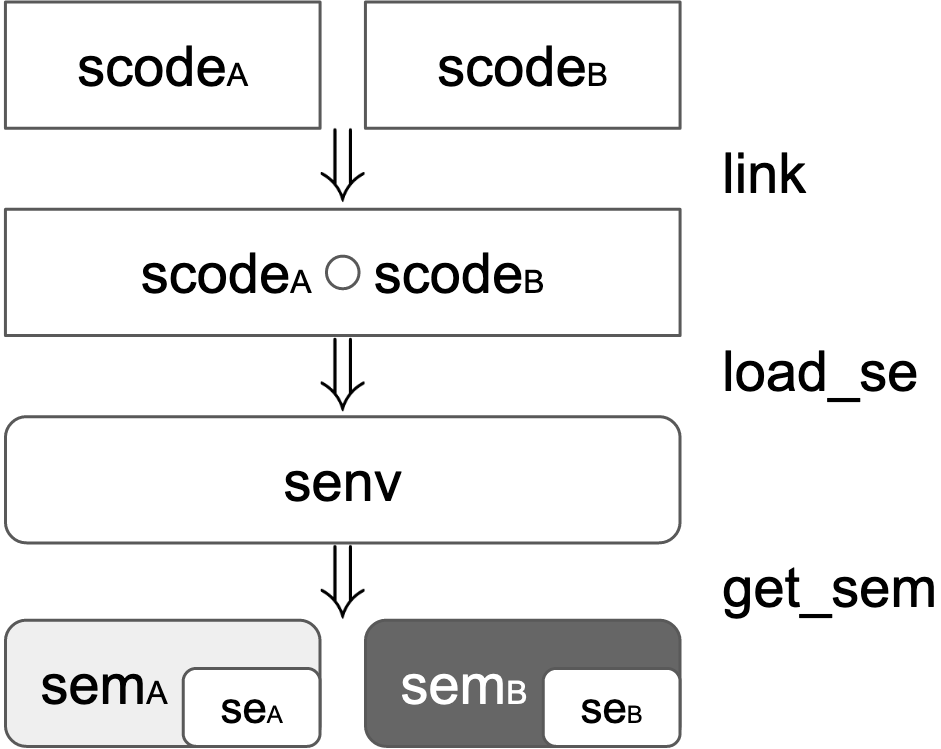
\includegraphics[width=0.25\linewidth]{fig-load.png}
%%   \caption{Loading Process}
%%   \label{fig:load}
%% \end{figure}



% Like \ccc{}, we require the set of states with \code{corestep}, states \code{at\_external}, and
% \code{halted} states are disjoint.  Second, unlike \ccc{}:



% Module semantics is almost same with \ccc{}. The differences are as follows.
% (i) While their primitives (\texttt{init\_core}, \texttt{at\_external}, \texttt{after\_external}, \texttt{halted}) were function, we use Prop instead.
% For \texttt{init\_core}, it is essential --- we have introduced nondeterminisim --- but for other cases, it is rather technical (and for uniformity with \texttt{init\_core}).
% Actually, we require the other three primitives are \emph{deterministic}, so it is equivalent with function.
% (ii) Our primitives change the memory, which is for marshalling/unmarshalling. In \ccc{}' marshalling/unmarshalling was hard-coded into \texttt{corestep} relation.
% (They already re-defined \texttt{corestep} for vertical compositionality.) In contrast, we just reuse off-the-shelf step relation from \cc{}.
% (iii) We support both C-style and Asm-style communications between modules, while \ccc{} only supported C-style.

% Currently, Asm-style communication is only allowed between Asm modules (this is the same for \ccx{}.

% Symbol code ($\Skel$) and symbol environment ($\Skenv$) represents \emph{language-agnostic} part
% of \cc{}'s program/global environment (as much as one can).
%% with one mild assumption --- each function has its signature --- which is true for all \cc{} languages.
% These are used in loading interaction semantics.  We use option signature type here.  The signature
% is none for the hand-written assemblies that does not follow (C-style?) calling convention, and for
% all other cases it is some.
%% We support both C-style and asm-style for call and return.

% We will skip explaining things that are same with \ccc{}.





% \myparagraph{Asm Wrapper Semantics}

% state recognition algorithm:
% \\ (1) PC points to my function --> corestep
% \\ (2) PC does not, but it is still in genv area --> call
% \\ (3) otherwise --> return

% Mention that unfree is somewhat special/nontrivial operation: it temporarily breaks \cc{}'s axiom, but it is okay.

% \begin{itemize}
%   \item init\_core:
%     \\ (1) c.(f) points to my function, fd. %% \cdashbox{It is declared as C-style and c is actually C-style} TODOOOOOOOOOOOOOOOOOOOO
%     \\ (2) PC <-| c.f
%     \\ (3) Allocate ``dummy'' stack with (size\_arguments fd.sig). Let its block id blk.
%     \\ (4) Fill in c.vs into blk
%     \\ (5) RSP <-| (blk, 0)
%     \\ (6) Assign junk blocks of arbitrary number
%     \\ (7) RA <-| arbitrary junk pointer outside genv area
%     \\ (8) Fill in other registers with junk pointer or arbitrary non-pointer
%   \item at\_external:
%     \\ (1) PC does not points to my function, but it is still in genv area.
%     \\ (2) From $se_{big}$, find signature of corresponding function.
%     \\ (3) Read list val from my arguments area, (vs).
%     \\ (4) Free my arguments area
%     \\ (5) c <-| (PC, current mem, vs)
%   \item after\_external:
%     \\ (1) $PC_{current}$ <-| $RA_{before}$
%     \\ (2) Make caller-save registers undef
%     \\ (3) RAX (return register) <-| r.v
%     \\ (4) Unfree my arguments area, and fill it with undef
%   \item final\_frame:
%     \\ (1) PC does not points to my function, and it is not in genv area
%     \\ (2) Check PC is same with initial RA
%     \\ (3) Do callee-save checking with inital registers.
%     \\ (4) Free my ``dummy stack''.
%     \\ (5) r <-| (r, current mem)
% \end{itemize}

% Mention we also support asm-style passing.
% As mentioned before, asm-style passing is only allowed between assembly modules.
% We just pass (both in call and return) current register set and memory directly.
% The only one exception is \textbf{RA} register: it exactly follows C-style convention, in order to use ``state recognition algorithm'' above.
% \textbf{RA} is \cc{}-specific pseudo register so we can do what we want.




%%% Local Variables:
%%% mode: latex
%%% TeX-master: "main"
%%% End:


\chapter{\;\;\;\;Formalization of Verification Techniques}
\label{sec:main-verification}

%% \todo{slight difference in math and coq dev ?}


%%% Local Variables:
%%% mode: latex
%%% TeX-master: "main"
%%% End:

{\newrevisioncmd
\section{Related Work}
\label{sec:related}

%% Besides \ccc{}~\cite{beringer:isem,stewart:ccc} and \ccx{}~\cite{gu:dscal,wang:saccx}, there are two
%% other lines of prior work on compositional correctness for CompCert.
%% Now we compare \ccm{} with each of the prior work.  The
%% comparison is summarized in \Cref{table:table1}.  \todo{explain each column.}
%% Left three columns describe characteristics of semantics, and right four columns describe that of
%% proof development.
%% \input{table1}

We discuss related work on compositional compiler correctness for \cc{} and other higher-order languages.

\subsection{Compositional Correctness for CompCert}

\myparagraph{\ccc{}} Besides what we have discussed, \ccc{}
introduces self-relatedness as a part of the notion of well-defined
context and shows refinement under well-defined contexts as a result
of the compiler correctness proof, whereas we uses such refinement as
a method to prove compiler correctness.  Also, the PhD thesis of
\cite{StewartThesis} observed, with a counterexample, one of the
three reasons for inadequacy of interaction semantics at assembly
level: not enforcing the assumption on the outgoing arguments area of
the stack. It informally concludes that assembly contexts should
respect the compiler's assumption without giving a formal solution.
Our repaired interaction semantics gives a formal way to enforce the
assumption by giving UB to those behaviors violating it.  The thesis
also suggests \emph{closed} specification modules (\ie without making
external calls) written in Coq's Gallina language, which foreshadows
our \emph{open} specification modules and verification against them.

\myparagraph{\ccx{}} Besides what we have discussed, the latest
version of \ccx{} \cite{wang:saccx} supports two features that \ccm{}
currently does not support. First, it proves that \ccx{} preserves the
stack consumption by instrumenting the languages' semantics to record
the size of the concrete stack frames. Second, it carries the compiler
correctness down to assembly with the flat memory model instead of
\cc{}'s block-based memory model. On the other hand, \ccx{} instruments the
languages' semantics to record permissions in the stack frames in
order to support address-taken stack variables, whereas \ccm{} supports
them, without instrumenting the semantics, by adding the private
memory components to memory injections as shown in
\Cref{sec:overview-verification:injection:dynamic}.
Interesting future work would be to apply the techniques of \ccx{} to \ccm{} to
support the two missing features, and conversely apply the technique of
\ccm{} to \ccx{} to support address-taken stack variables without
recording permissions on the stack.

\myparagraph{\scc{}}
%
\scc{}~\cite{kang:scc} proves a weaker form of compositional correctness for \cc{},
namely correctness of separate compilation.
Specifically, the proof assumes that all modules
are separately compiled by the \emph{same} compiler and then linked
together without linking with any handwritten assembly.
%% and exploits the fact that all main optimizations are performed on the RTL intermediate language.
For this, \scc{} employs a surprisingly lightweight \emph{closed} simulation technique,
which, therefore, has been officially adopted by \cc{} since version 2.7.
%% Consequently, the verification technique is surprisingly lightweight
%% and thus has been officially adopted by \cc{} since version 2.7.
%% Its ``Level B'' verification of RTL optimizations uses the standard contextual refinement in RTL.
%% \scc{} has been officially adopted by \cc{} from version 2.7.

%% can be considered as an
%% instance of RUSC, but with a significant restriction: all contexts should be RTL modules, rather
%% than arbitrary modules in arbitrary interaction semantics that are self-related by parameterized
%% relations.

% SepCompCert

% - them: RTL contexts
% - us  : defined "good" contexts,


% but it also has two fundamental restrictions: it cannot support (i) a multi-language program, and
% (ii) adding a new compiler (with different intermediate languages). Their technique to prove
% ``Level B'' correctness has inspired us to develop RUSC: actually their technique can be
% understood as a special case of RUSC where RTL is the only end-language.
%
% intentionally aim at a less ambitious goal than ours---verifying compositional correctness for a
% \emph{single} compiler only.



%% Finally, whilst their implementation is very lightweight in current
%% \cc{}, they do impose additional complexity in global optimizations,
%% which potentially burdens future extensions of \cc{}.  We will discuss
%% this point in \Cref{sec:TODO}.

%% Thanks to \scc{}, \cc{} now has a soundness theorem for
%% separate compilation, with syntactically linked assemblies as its
%% target program.  To put it another way, \cc{} trusts their target
%% program an appropriate, closest formalization of actual physical
%% behavior, and we follow this stance.  \todo{Email Valex?}


%% \myparagraph{\ccx{}}
%% %
%% \ccx{}~\cite{gu:dscal,wang:saccx} extends \cc{} to support multi-language programs, but as discussed
%% in \Cref{sec:introduction}, it is highly specialized for the CertiKOS~\cite{CertiKOS11,CertiKOS16} verification
%% project.  As a consequence, it has interesting pros and cons compared to \ccm{}.

%% On the one hand, \ccx{} imposes several restrictions on the input modules, in order to reduce its
%% verification to closed simulation and reuse most of the verification in the original CompCert.
%% Specifically, \ccx{} imposes the following restrictions on the input modules.  First, it assumes all
%% the input modules (either in C or assembly) are verified against certain specifications, called
%% Certified Abstraction Layers, and proves that the compiled assembly programs also satisfy the same
%% specifications.  Second, it disallows non-terminating functions and mutually recursive modules.
%% Third, it requires semantics to be deterministic.  Fourth, as a consequence, it supports Clight,
%% which is a deterministic intermediate language in CompCert, rather than CompCert C, which is the
%% nondeterministic source language of CompCert. \jeehoon{What does it mean by CompCertX disallowing
%%   events?}

%% On the other hand, \ccx{} supports more advanced control flows, such as context switch or
%% coroutines, than just function call and return supported in \ccm{}.  We expect we can extend \ccm{}
%% to support for those features by generalizing interaction semantics and RUSC, but we leave it as
%% future work.

% CompCertX

% - intro에서 언급
% - 제약을 해서 본질적으로 closed simulation을 쓸 수 있도록 함
% - 소스가 검증되었다고 가정 (closed program, closed simulation)
% - 검증이 mutual recursion 지원 안함
% - (module local reasoning 안됨?)
% - deterministic, no event (open spec?)  syscall에 대해 axiomatic하게 closed semantics 줌
% - Clight?
% - 장점: 다른 control flow 지원 (context switch, coroutine, ...)
%   we expect, future work, ...

% First restriction is that it does not allow modification of caller's stack if the caller is in
% another module.  Second restriction is that in order to use their correctness theorem, each function
% should have its corresponding \text{primitive specification}, which disallows (i) callback
% (recursive call) between modules, (ii) infinite behavior, (iii) producing an event, and (iv)
% nondeterministic behavior.  Even with these restrictions, \ccx{} was sufficient for their OS
% verification, but as the authors made it clear in the paper, ``\ccx{} can not be regarded as a full
% featured separate compiler for CompCert.''. Recent progress in this project \cite{wang:saccx}
% removes the first restriction (stack modification), but instead it changes the memory model of \cc{}
% and led to relatively heavier development.

% \ccx{}~\cite{gu:dscal} extends \cc{} to support multi-language program, but it is specialized for
% their OS verification project and has several restrictions.  First restriction is that it does not
% allow modification of caller's stack if the caller is in another module.  Second restriction is that
% in order to use their correctness theorem, each function should have its corresponding
% \text{primitive specification}, which disallows (i) callback (recursive call) between modules, (ii)
% infinite behavior, (iii) producing an event, and (iv) nondeterministic behavior.  Even with these
% restrictions, \ccx{} was sufficient for their OS verification, but as the authors made it clear in
% the paper, ``\ccx{} can not be regarded as a full featured separate compiler for CompCert.''. Recent
% progress in this project \cite{wang:saccx} removes the first restriction (stack modification), but
% instead it changes the memory model of \cc{} and led to relatively heavier development.

% Concerning proof development, they also relied heavily on vertical
% composition of memory relations. Therefore, we \todo{rephrase:} think
% adding the Unreadglob pass would require a major change to their proof
% architecture, if it is possible. Also, their development is not based
% on the latest \cc{} and is not complete, omitting Unusedglob
% optimization and frontend (from C to Clight). \todo{connective} Their
% development is roughly divided into two parts: one is \ccx{} which
% extends \cc{} but without explicit notion of linking, and the other is
% layer calculus library which actually introduces the notion of
% linking.  The former comprises 9K lines of Coq, which is almost as
% small as our language/pass-specific development. The latter comprises
% at least \footnote{Its LOC is calculated with
%   \href{https://github.com/DeepSpec/dsss17/}, the only publicized
%   source code we could found, but it seems they do not contain
%   everything: \eg assembly style primitives} 30K lines of Coq, so in
% total their development is of similar size with ours.

% %29851 exactly

% \note{2019년 1월 publish, compcert 버전은 2017-02. 2년치 업데이트 안함}

%% \todo{SACCX claims their implementation is complete, but it is NOT!}



%% \input{fig1} In a broad sense, there are three remarkable works
%
% For past few years, about three remarkable works has been accomplished in this area --- extending
% \cc{} to support some form of compositional correctness. To this end, each of them developed their
% own notion of multi-module semantics, and extended \cc{}'s proof under the proposed semantics. We
% will first discuss them, then discuss two more works that are related in a broad sense ---
% tackling the same problem, but outside the \cc{}.
%
%% We will discuss them first, and then discuss one more work that tackles compositional compiler
%% correctness, but that are related in a broad sense.  However, none of them were both
%% \textit{sound} and \textit{general}.

% \myparagraph{\ccc{}}
% %
% The last one is \ccc{} \cite{beringer:isem, stewart:ccc} which developed the interaction
% semantics. As discussed in this paper, their semantics is unsound \cite{sec:sec:overview-semantics}
% and development was heavyweight. They used \cc{} v2.1 as a baseline, which lacks challenging passes
% such as Unusedglob and ValueAnalysis, and did not port frontend (C to Clight). Finally, as they
% fixed one memory relation for the whole proof, adding a new pass that requires more powerful memory
% relation would require a major change.


\myparagraph{\cascc{}}
%
%% > Line 1199: You write that CASCompCert has the restriction that
%%   "stack allocated data should not be address taken."  I believe this
%%   is true of the PLDI paper and the Coq proofs attached to it, but
%%   they have a longer tech report cited from the PLDI paper with many
%%   pages of Latex explaining how it would be possible to build Coq
%%   proofs that remove this restriction.  Does that mean you accurately
%%   characterize their work?  Yes, probably; but it may not be an
%%   _inherent_ limitation of their approach.
%% >  Furthermore, the claim (line 1998) that Jiang et al's approach forbids
%%   address-taking of stack-allocated data is incorrect: while their Coq
%%   formalization and the paper main paper indeed do not consider
%%   leakage of stack pointers, the associated TR describes (without Coq
%%   formalization, but with 30 pages LaTeX proof) how escaping stack
%%   pointers can be supported (with more overhead).

%% > while the recent PLDI paper by Jiang et al (CASCompCert) is
%%   mentioned, its characterization hardly does it justice: indeed, the
%%   PLDI paper provides an abstract rephrasing of CompCompCert's
%%   rely/guarantee framework (hence the present paper's key criticism of
%%   CompCompCert may well apply to it, too), but it then uses the
%%   abstract framework to establish compiler correctness in the presence
%%   of concurrency. In contrast, the present paper does not treat
%%   concurrency at all, and hardly discusses it.

%% Thanks for pointing this out. We will also cite and explain the technical report.

%% We agree with this point. We will say that CASCompCert demonstrates
%% that the technique of CompCompCert applies to the concurrency setting
%% while we have not demonstrated applicability of our technique to
%% concurrency yet.

%% extends \ccc{} in three dimensions:
%% \textbf{C}oncurrency, \textbf{A}bstraction, and \textbf{S}eparate
%% compilation (hence the name).
%% However its main focus is on concurrent
%% abstraction, not on compositional correctness.
%% In the view point of
%% compositional correctness, \cascc{} basically follows the approach of
%% \ccc{} and simplifies its complexity by imposing a significant
%% restriction. Specifically, there are three problems.
%% suffers from two problems.
%% making a few unrealistic assumptions on compositional correctness.
%% its semantics of physical linking is unsound just like that of \ccc{}.
%% First, since it uses the original interaction semantics, its adequacy
%% w.r.t. assembly and C does not hold.
%% Second, it tames the complexity
%% of structured simulations of \ccc{} by requiring the restriction that
%% stack allocated data should not be address taken: this restriction
%% unnecessitates the use of memory injection.
%% Third, it covers only
%% those passes the first \ccc{} covered, which means it covers only 12 out
%% of 20 passes in CompCert 3.0.1, which is their base version.

\cascc{}~\cite{jiang:cascc} extends \ccc{} to support concurrency in
the absence of data races, which demonstrates that the proof technique
of \ccc{} (\ie structured simulations) scales to a
concurrent setting.  However, in the Coq formalization, \ccc{} tames
the complexity of structured simulations by $(i)$ not allowing
address-taken stack variables (although how to support them using
structured simulations is described with paper proofs in the
associated technical report\footnote{\url{https://plax-lab.github.io/publications/ccc/ccc-tr.pdf}}); and $(ii)$ only
covering 12 out of the 20 passes in its base version, CompCert 3.0.1
(although the 12 passes are exactly those that are covered by the
original \ccc{}): these restrictions unnecessitate the use of memory
injection. Also, \cascc{} can only allow special nondeterminism caused
by scheduling threads by slightly relaxing the conditions for forward
simulation, while \ccm{} can allow arbitrary nondeterminism by mixing
forward and backward simulations.

We do not currently see any problem with applying the approach of
\cascc{} to \ccm{} to support concurrency in the absence of data races.
Moreover, we expect that the compiler verification technique for
\emph{promising semantics}~\cite{Kang:promising}, which is also based
on simple closed simulations, applies to \ccm{} to fully support
relaxed-memory concurrency.

%% it addressed the
%% nondeterminism inherently arising in concurrency or linking only in a restricted fashion.
%% Specifically, it generalizes forward simulation to support for the nondeterminism, instead of
%% applying backward reasoning, but its use of forward simulation does not apply to genuinely
%% nondeterministic cases like relaxed-memory concurrency.
%% Third, it requires all optimizations to be
%% verified using an open simulation with memory extension, and disallows verifiers to reason about
%% optimizations using different memory relations.\footnote{Note that \ccc{} requires
%%   all optimizations to be verified using an open simulation with memory injection.}
%% Fourth, to
%% verify optimizations with memory extension, it disallows the use of a large class of memory
%% operations.  Specifically, it disallows programmer to take the address of stack variables, and
%% designates heap allocation (\texttt{malloc}) and deallocation (\texttt{free}) operations as visible
%% events, thereby forbidding optimizations on those operations.

%% Lastly, it covers only those passes
%% that are covered in \cite{stewart:ccc} at the time that it is published.

% \youngju{simplifying assumption - unsound 매치가 안되는 것 같습니다}
% \\
% \youngju{nondeterminisim이 linking에서 일어나지는 않을겁니다 -- 얘들은 unsound한거 해결을 안해서 nondeterminisim 넣을 필요가 없었습니다.}
% \\
%% \todo{Also mention \ccc{} does not support malloc/free optimizations.}
%% \\

% CASCompCert

% - focus on concurrency, simplified the problem of compositionality
% - open simulation
% - memory relation을 extension으로 fix, vertical/horizontal compositionality
% - heap: malloc, free을 다 external function call
% - stack: no memory (register), address not taken
% - compcomp original paper에서 한 패스만 커버
% - semantics도 버그 답습 (physical linking)
% - nondeterminism: forward -> backward가 되는 상황. 계속 forward로 증명. "switch point"라는 개념을 semantics에 넣음
%     + 우리는 backward로 하는게 꼭 필요했던 상황


% In order to focus on the new challenges they faced, they inherited development of \ccc{} as much
% as possible.  Consequently, they also inherited the problem of \ccc{}: their semantics is unsound
% in the same way.  For proof development, they avoided the challenges we faced by (i) employing
% restricted semantics (each module has separate memory space, so passing a stack pointer to another
% is prohibited), which made their local simulation \todo{simpler? trivial? 약간 부정적인 단어로?},
% and (ii) not porting complex optimizations including Inlining (which enforced \ccc{} to strengthen
% their structured injection), all the passes using ValueAnalysis, and Unusedglob.  Still, they had
% to re-implement passes using identity relation to use extension relation.  Finally, they pointed
% out that taming nondeterminism was one of their four major challenges. They addressed it but (i)
% their nondeterminism is in certain form --- which can be understood as a special case of
% determinate/receptive --- thus they reasoned it using forward simulation, and (ii) it is baked in
% their simulation definition and they do not developed a reusable metatheory.

%% It provides semantics to a multi-language program, and without any restrictions imposed in \textit{contextual compilation}.
%% Therefore, \textit{interaction semantics} is strictly more powerful than \textit{contextual compilation}\cite{wang:saccx}.
%% Also, they invented a \mrel{} called \textit{structured injection}, which is significantly more sophisticated than \cc{}'s vanilla \textit{injection}. \todo{For what?}
%% %% They proved its veritcal and horizontal compositionality
%% However, this comes with an expensive cost.
%% First, their development caused devastating change on \cc{}'s code base.
%% They had to rewrite both semantics and proof.
%% %% For semantics, they annotated step with extra event structure,
%% %% and they added two extra states for low-level languages dedicated for \textit{marshalling} in and out.
%% %% For proof, they had to develop a sophisticated \mrel{} called \textit{structured injection} which is significantly more complex than \cc{}'s vanilla \textit{injection}.
%% For proof, they had to replace each translation's \mrel{} into \textit{structured injection}, invalidating the strength of using multiple \mrel{}s.
%% This resulted in much more complex proof for each optimization, \eg{} ``CleanupLabelsproof'' became 2043 LOC while it was only 372 LOC in vanilla \cc{}.
%% As a consequence of such heavyweight changes, it became very hard to maintain compatibility with up-to-date \cc{}.
%% In fact, their development is no longer maintained since 2015 \footnote{https://github.com/PrincetonUniversity/icc}, with their version remaining in 2.1 while \cc{} has updated to 3.5.
%% Second, more importantly, their semantics is unsound. Their proof lacks \lbound{}, and it actually does not hold! We will describe this more in the \Cref{sec:TODO}.
%% \todo{their paper lacks 3 passes / they are implemented after paper / SACCX attacks it}



%% Finally, in terms of \textit{extensibility}, all three existing works are more or less rigid.
%% By \textit{extensibility}, we consider both dimensions of extension,
%% which we call \textit{horizontal extensionality} (adding a new verified compiler)
%% and \textit{vertical extensionality}
%% (adding a new compiler optimization, possibly with totally different \mrel{}).
%% \scc{} is not horizontally extensible, as they manifested in their paper.
%% The simplest scenario this could be troublesome is compiler version upgrade.
%% Its soundness theorem does not guarantee you anything when you link assemblies from different versions of \cc{}.
%% %% Also, to the best of our knowledge, it is unclear whether \ccx{} and \ccc{} are vertically extensible.
%% On the other hand, \ccx{} and \ccc{} are not vertically extensible with ease.
%% Their development relies heavily on the vertical composition of \mrel{}s
%% (vanilla injection and \textit{structured injection}, respectively).
%% It is unclear if we can add an optimization pass
%% which uses \mrel{} that does not compose with injection (or \textit{structured injection}, respectively).
%% A specific example of such optimization is given in \Cref{sec:TODO}.
%% However, our development is extensible in both dimensions.
%% We will clarify this in \Cref{sec:overview}.



\subsection{Compositional Compiler Correctness for Higher-Order Languages}

\myparagraph{Pilsner}
%
Pilsner~\cite{neis:pilsner,pb} is a multi-pass optimizing compiler from
a higher-order imperative language down to an idealized assembly language.
%% supporting horizontal and vertical compositionality.  
To verify horizontally and vertically compositional correctness in the presence of higher-order functions, Pilsner uses
very general and flexible open simulations, called \emph{parametric simulations},
whose vertical compositionality proof is also technically very involved.
%% But as a consequence, its vertical compositionality
%% proof is significantly more complicated than that of \ccm{}, which is straightforward from the
%% transitivity of (behavior) set inclusion.
Since it would be hard to define interaction semantics
due to the different representations of values and
memory in the source and target languages,
the RUSC technique is unlikely to be applicable to Pilsner.
%% Pilsner aims higher than \ccm{} in
%% that higher-order functions are not supported by interaction semantics
%% and thus is beyond the reach of RUSC.

Also, our approach to reasoning about dynamically and statically
allocated local memory, presented in \Cref{sec:overview-verification},
follows that of Pilsner, which is based on the work of
\cite{DBLP:conf/icfp/DreyerNB10}. A minor difference is that we
simplify the formulation by restricting the occurrence of private
transitions only to just before and after external calls, while
Pilsner allows private transitions at every local step only requiring
public transitions between the end-to-end worlds of the execution of a
function.

%% Unlike \cite{DBLP:conf/icfp/DreyerNB10,pb}, for simplicity, we restrict
%% the occurrence of private transitions only to just before and after external function calls.


\youngju{앞에서 RUSC는 interaction semantics에 연관된 개념이 아니라
  임의의 multi-language linking operator에 대해서 동작하는거로
  이야기했습니다. 저 세팅에서는 linking operator를 정의하기 어려운게
  문제의 본질인 것 같습니다.}

% \youngju{(i) compositional correctness for \cc{} (ii) compositional
%   compiler correctness 가 자연스러운 것 같고 그냥 compositional
%   correctness는 어색한 것 같습니다.}

% Pilsner

% - higher-order language, interaction semantics 정의하기 어렵고 (value, register, ... 등등이 달라서) RUSC 어렵다.
% - open simulation을 굉장히 flexible하게 general하게 정의했다
% - vertical composition 증명이 어렵다


\myparagraph{Multi-language semantics}
%
Ahmed and her collaborators propose multi-language
semantics~\cite{perconti:multilang,patterson:funtal,DBLP:conf/fossacs/SchererNRA18,New:2016,ICFP19}
as an approach to prove compositional correctness and full abstraction
of a compiler for both assembly-like and higher-order languages.
Specifically, they define a language that combines all of the source,
intermediate and target languages, and prove contextual equivalence
and/or full abstraction for each translation pass in the combined
language using logical relations (with back-translations).  In this
approach, they rule out ill-formed contexts by syntactic type systems
and use the typed contextual equivalence for compositionality.  Since RUSC
rules out ill-formed contexts by semantic program relations, it would
be interesting to see if RUSC could be applicable and beneficial to
the approach of Ahmed \etal, in particular, for full abstraction.

%% >  extending the comparison between RUSC and contextual refinement: is
%% >  it possible to formulate a variant of full abstraction w.r.t. the set
%% >  \cal{R} and show that it is satisfied by RUSC? This would relate to
%% >  Patterson & Ahmed's recent discussion (ICFP'19) of full-abstraction,
%% >  and the need to complement it by notions that take low-level
%% >  equivalences into consideration.

%% The idea of applying RUSC to the full abstraction setting sounds
%% interesting. We did not have a chance to think about how RUSC can be
%% used to increase modularity of full abstraction proofs yet.  We will
%% think about it and if we have interesting ideas, we will discuss them
%% in the future work section. Thanks!

%% This approach is still closed in the sense that it does not support contexts written in other languages that are
%% not embedded in the combined language.  In contrast, RUSC is open in the sense that it supports
%% arbitrary self-related contexts written in arbitrary interaction semantics, even including
%% mathematical specifications as shown in \Cref{sec:overview-modulelocal}.



% \youngju{semantics를 correctness를 위한 approach로 본다는게 어색한 것 같습니다.}

% \youngju{(i) compositional correctness for \cc{} (ii) compositional
%   compiler correctness 가 자연스러운 것 같고 그냥 compositional
%   correctness는 어색한 것 같습니다.}

% TODO: Amal Ahmed

% - fix된 language, language 자체를 잘 제약해서 contextual refinement
% - closed (multi-)language w/ contextual refinement <-> open language w/ RUSC
% - 우린 context에 spec도 넣을 수 있음 (구체적으로 programming reasoning)


% \todo{
%   할 이야기
%   - semantics 정의 --> syntactic. 하지만 inline assembly 허용
%   - unsoundness --> toy language 다
%   - proof --> contextual equivalence
%   -
% }


%% \section{Conclusion and Future Work}
%% \label{sec:conclusion}
}

%%% Local Variables:
%%% mode: latex
%%% TeX-master: "main"
%%% End:


%% \chapter{\;\;\;Introduction}
%% \label{chap:intro}
%% \section{Introduction}\label{sec:introduction}

%% \jeehoon{In title, maybe no space before colon?}

\cc{} \cite{CompCert, Compcert-CACM}, the first \emph{verified}
\emph{optimizing} compiler for \emph{the C programming language}, has
served as a backend in end-to-end verified
software~\cite{appel2014program}. Specifically, \cc{} compiles programs written in (a
large subset of) C down to assembly code via various translation
passes including a number of common optimizations.  Moreover, it is
formally verified in Coq that every translation of \cc{} preserves the
semantics: the generated assembly code behaves as specified by the
semantics of the source program. Therefore, \cc{} has been used to
transform verification results about the source C program into those
about the compiled assembly code in various projects such as
CertiKOS~\cite{CertiKOS11, CertiKOS16} and VST~\cite{VST}.

There is, however, a limitation in the original \cc{} that restricts
its application to a more wide range of software verification---namely
the lack of support for handwritten assembly. This
limitation can be serious in verification of \emph{real-world}
software because handwritten assembly is often crucial for writing
low-level system software or library code.

To overcome this limitation, two extensions of \cc{}, namely \ccx{}
\cite{gu:dscal,wang:saccx} and Compositional CompCert (shortly, \ccc{}) \cite{beringer:isem,stewart:ccc}, have
been developed. Interestingly, they take different approaches to
\emph{two key challenges}:
\begin{enumerate}
\item how to modularly verify each translation of each
module using a different relational memory invariant (shortly, memory relation) and compose the proofs all
together; and
\item how to deal with illegal interference from
arbitrary (handwritten) assembly modules that can invalidate compiler
translations of C modules (\eg not preserving the
callee-save register values).
\end{enumerate}

\revision{%
We elaborate more on the first, more fundamental, challenge.
\cc{} uses three different memory relations called memory \emph{identity},
\emph{extension} and \emph{injection} (in the order of complexity and generality)
for a proof engineering purpose: it uses a
simpler relation whenever possible to simplify the correctness proof.
%
The challenge occurs in an open setting where a translation of an
open module is verified separately. In a closed setting as in \cc{}
where the whole closed program (\ie all the modules) is compiled by the
same translation pass thereby being verified as a whole,
verification of such a closed program using a simpler relation essentially implies
that using a more general one.  However, in an open setting (\ie for
verification of an open module), that implication does not hold
because such verification assumes that the unknown contexts also
preserve the same memory relation. In other words, using a simpler
relation, the verification guarantees a stronger property on its own
module but assumes a stronger property on the context modules.
Therefore, verification of open modules using different memory relations
cannot be compared, which makes composition of such verifications hard.%
}

\myparagraph{\ccx{}'s Approach}
%
\ccx{} is developed as a backend compiler for the verified OS kernel
\certikos{} \cite{CertiKOS11,CertiKOS16} and thus specialized for this purpose.
Specifically, \ccx{} simplifies the two challenges by making two
assumptions that $(i)$ there are no mutual dependencies among the
input modules and $(ii)$ each input module is verified against a
well-behaved specification, called \emph{Certified Abstraction Layer (CAL)}.

First, these assumptions enable \ccx{} to use \emph{closed}
simulations, the simple verification technique used by the original
\cc{}. The simulations are closed in the sense that they relate known
source and target functions under the condition that all invoked
unknown functions have independent good behaviors.
\revision{%
Specifically,
the unknown functions $(i)$ provide full end-to-end behaviors
regardless of who the caller is (\ie whether it is the source or the target);
%% the end-to-end behaviors of the unknown functions $(i)$
%% do not depend on who the caller is (\ie whether it is the source or the target)
and $(ii)$ those behaviors satisfy a certain good-behavior property.
%% The reason why
%% \ccx{} can use closed simulations is because the two assumptions of
%% \ccx{} above imply those two for closed simulations,
%% respectively.
Note that these two requirements for closed simulations directly
follow from the two assumptions of \ccx{} above, respectively.
Then proving compositionality between closed simulations
using the three different types of memory relations
%used in \cc{}
%% (\ie memory identity, extension and injection)
is straightforward
as discussed above (\ie verification using a simpler relation
implies that using a more general one).%
}
%% not so involved thanks to the closedness assumptions.
As a result, the correctness proofs of
all compiler passes using closed simulations in \ccx{} are only 15.51\% larger than
those in the original \cc{}~3.0.1 in terms of significant lines of code~(SLOC)\footnote{we counted SLOC using \texttt{coqwc}.},
and the metatheory \revision{(\ie all the rest)} is 47.65\% larger.

Second, thanks to the assumptions of \ccx{}, interference from
assembly modules is also handled simply.  The assumption that
handwritten assembly modules are verified against CAL specifications
implies that those modules do not cause any illegal interference (\ie
well-behaved).

\myparagraph{\ccc{}'s Approach}
%
\ccc{} establishes a more general correctness result \mbox{without}
the restrictions of \ccx{} but at the expense of using a more
heavyweight verification technique of its own, called \emph{structured
  simulations}. They are in the form of \emph{open} simulations in the
sense that they allow invoked unknown functions to depend on their
callers (\eg via mutual recursion). Since this openness technically
makes compositionality proofs much harder as discussed above, to simplify them \ccc{}
uses a single memory relation, called \emph{structured injection}.
For this reason, the verification technique is less flexible.
Specifically, the proofs of the whole compiler passes using the
structured injection deviate quite far from the original proofs in
\cc{} and require significantly more efforts: the correctness proofs
of all compiler passes are 145.77\% larger than those in the
original \cc{}~2.1, and the metatheory is 81.77\% larger.

Also, \ccc{} handles interference from assembly modules more
generally without assuming the good-behavior property for input modules.
Since such interference only occurs via the register file
and the function arguments area of the stack (\ie the shared resources
that exist in assembly but not in C), the \emph{interaction semantics}
of \ccc{}, which gives a logical semantics to programs consisting of
multi-language modules, duplicates those resources for each invocation
of an assembly module and does not propagate any illegal effects
outside the module.

However, the treatment comes with no adequacy proof with respect to
the physical semantics. Indeed, interaction semantics is not
adequate: due to the logical isolation of illegal effects, the
interaction semantics of linked assembly modules deviates from their
\emph{physical} semantics (\ie the assembly semantics of \cc{}) when
one of the modules indeed causes illegal interference, for example, by not
preserving the callee-save register values.
\revision{Note that this problem was also observed and discussed
in the PhD thesis of \cite{StewartThesis} (see \Cref{sec:related} for comparison).}

Finally, there is another difference between \ccc{} and \ccx{}:
\ccc{} only supports C-style calling conventions, while \ccx{} additionally
supports assembly-style calling conventions (\ie imposing no conditions
except on the return address) between assembly modules.

\myparagraph{Our Approach}
%
In this paper, we develop a new framework achieving both the
flexibility of \ccx{} and the generality of \ccc{}.  We demonstrate
its power as a compiler verification framework by applying it to \cc{}
but also as a program verification framework with interesting
examples, for which we write mathematical specifications as abstract
modules in interaction semantics and prove refinement between the
examples and their specification modules.  Specifically, we develop:
\begin{itemize}
\item Open (Mixed) Simulations: a simpler version of structured simulations,
  $(i)$ allowing arbitrary memory relations including memory identity, extension and injection,
  and $(ii)$ supporting mixed forward-backward simulation;
\item RUSC (Refinement Under Self-related Contexts): our new
  lightweight theory for composing arbitrary open simulations
  together, which is the highlight of our theoretical contribution;
\item Repaired Interaction Semantics: providing adequacy w.r.t. the
  physical semantics and additionally supporting assembly-style
  calling conventions;
\item \ccm{}: the latest version of \cc{} (v3.5) fully extended with
  the repaired interaction semantics and open simulations to support
  multi-language linking (\newrevision{18.73}\% larger in the correctness
  proofs of all compiler passes, and \newrevision{32.59}\% larger in the metatheory);
\item \texttt{Unreadglob}:
  %% a new optimization pass we added requiring
  %% a new kind of memory relation, memory injection with module-local
  %% invariants, where \texttt{Unreadglob} eliminates all unread static
  %% variables and instructions writing to them;
  a new optimization pass we added that eliminates all unread static
  variables and instructions writing to them,
  whose verification for \emph{open} modules requires
  a new kind of memory relation, \emph{memory injection with module-local
  invariants};
\item \texttt{mutual-sum}: an example consisting of $(i)$ C and
  handwritten assembly modules that mutually recursively compute
  summation up to a given integer, performing memoization using
  module-local static variables, and $(ii)$ correctness proofs
  against their specification modules using open simulations with the
  new memory relation, memory injection with module-local invariants;
\item Verification of \texttt{utod}: providing a correctness proof
  against its specification module using an open simulation,
  %% with the original memory injection,
  where \texttt{utod} is a handwritten
  assembly function casting unsigned long to double, whose correctness
  against its specification is axiomatized in \cc{} but not any more
  in \ccm{}.
  % (see \Cref{sec:utod-verification} for details).
\end{itemize}
\medskip

The key theory enabling all these results is RUSC, which takes a set
of (almost arbitrary) open simulations $\rels$ and lifts them to a
larger relation $\rusc_\rels$ that is fully compositional.
\newrevision{The idea is inspired by the situation where
  the transitivity problem of logical relations is avoided
  by proving their inclusion in the contextual refinement,
  which is trivially transitive.}
To increase its applicability, RUSC simply generalizes the notion of contextual refinement~(CR)
%% of RUSC is to generalize the standard notion of contextual refinement~(CR)
by parameterizing over a set of program relations $\rels$.
Specifically, we say that $p \rusc_\rels q$ if for any
context $C$ that is related to itself by every relation in $\rels$,
the observable behaviors of $C[p]$ are refined by those of $C[q]$.  The
key idea is to give the notion of well-behaved contexts w.r.t. a set
of program relations~$\rels$ as those that are self-related by every
relation in $\rels$. The intuition behind it is that a context
self-related by a program relation $R$ preserves all the invariants of
the relation $R$.  The merits of RUSC are that RUSC is $(i)$ unlike CR,
applicable even in the presence of ill-behaved contexts,
which is the case in our setting, and $(ii)$ fully compositional like
CR.  By setting $\rels$ as the set of open simulations with four kinds
of memory relations---the three relations used by \cc{} and our new
relation, memory injection with module-local invariants---we can
freely choose one of them in verification of a compiler pass,
or a program against its specification.

%%
%% However, the magic in our approach is that we do not need to prove vertical compositionality of open simulations at all.
%% Instead, vertical compositionality comes from the RUSC relation, whose proof is trivial.
%% It is similar to the situation where logical relations are not transitive, but the contextural refinement including them
%%  is transitive, whose proof is trivial.
%%

Also, to generally support forward simulation in the presence of nondeterminism,
we implement
the notion of mixed forward-backward simulation from \cite{neis:pilsner}
with a slight generalization needed for \cc{}
(see \Cref{sec:overview-verification:mixedsim}).

We repair the interaction semantics of \ccc{} by defining those behaviors causing
illegal interference as \emph{undefined behaviors}~(UBs)\footnote{\revision{UBs
  can be understood as forbidden behaviors, so that compilers
  are licensed to translate them into \emph{any} behaviors.}}, which,
however, required a few nontrivial ideas. First, we identify the
sources of inadequacy of interaction semantics as those behaviors
violating three assumptions---seen as a part of the official calling convention---made
by standard compilers such as GCC and LLVM with concrete counterexamples.
Second, to make those illegal
behaviors UBs, we strengthened only the interaction part of
interaction semantics without changing the underlying language
semantics of \cc{}, which indeed is quite nontrivial as
discussed in \Cref{sec:overview-semantics}. Finally, we
prove two adequacy results: $(i)$ the interaction semantics of linked
assembly modules is refined by their physical semantics, and $(ii)$
the physical semantics (\ie the language semantics of \cc{}) of linked
(typed-checked) C modules is refined by their interaction semantics.
%% These results mean that the repaired interaction semantics is not too
%% small and not too big.
\revision{%
These results mean that the repaired interaction semantics
does not give too few behaviors to assembly programs (\eg missing physically observable behaviors),  
nor does it give too many behaviors to well-typed C programs (\eg giving UB to them).%
}

\ccm{} is a full extension of \cc{}~3.5 without missing any
translation pass and without changing the underlying semantics,
which is developed in two steps. First, \revision{we refactored the proofs of
the original \cc{} to get \ccr{}, 
%% in the style of open simulations
where the main parts of the correctness proof of each pass
is separated out as a main lemma that
can be later used for both closed and open simulation proofs.}
\ccr{} gives exactly the same results as \cc{} with only 4.41\%
increase in the correctness proofs of all passes and 2.74\% increase in
the metatheory. Then, on top of \ccr{}, we developed an add-on
package, \ccm{} pack, supporting interaction semantics and multi-language
linking. \ccm{} reuses all the main lemmas of \ccr{} and adds $(i)$
additional proofs to reason about the interaction parts of
interaction semantics in the correctness proofs of all passes, which amount to
14.32\% of the original proofs in \cc{}, and $(ii)$ additional
metatheory including interaction semantics and RUSC, which
amounts to 29.85\% of the original metatheory in \cc{}.

The three applications, \texttt{Unreadglob}, \texttt{mutual-sum} and
verification of \texttt{utod}, show the flexibility of our framework:
allowing arbitrary memory relations and mathematical specification
modules. In particular, to the best of our knowledge, our work is the
first verification, in the context of \cc{}, that reasons about module-local static
variables with private invariants that can be modified across external function calls (due to
mutual dependence between multiple modules) .

The Coq development is available at:
\[ \text{\url{https://sf.snu.ac.kr/compcertm}} \]

The remainder of the paper is structured as follows.
We give a high-level overview of the main ideas in
\Cref{sec:overview-verification}-\Cref{sec:overview-modulelocal};
the main results of \ccm{} and an analysis of its development in \Cref{sec:results};
its formal details in \Cref{sec:main-semantics}-\Cref{sec:main-verification};
and a comparison to related work in \Cref{sec:related}.

%% \todo{Intro:
%%   make three points about sound semantics.
%% }

%% \ccc{}'s verification was costly: while baseline \cc{} comprises 112K
%% lines of Coq, they developed \emph{additional} 122K (109.1\% compared
%% to the baseline) lines of Coq. What is worse is that majority of such
%% overhead is caused not by metatheory but by \emph{re-implementation}
%% of each language's semantics and each passes' proof (77K lines of Coq,
%% 125.8\% compared to the corresponding baseline). This is indeed
%% problematic because a compiler evolves over time (modifying, adding
%% optimizations and sometimes adding a new source/target language) and
%% keeping the development up-to-date is a significant overhead.

%% \todo{
%%   - our solutions:
%%     + change semantics:
%%       (1) essential: justified by calling convention.
%%       (2) challenging: require new (nontrivial) semantics and proof techniques
%%       (3) justify: upper bound.
%%     + lightweight verification
%%       (1) truly modular verification technique (in the setting of CompCert languages)
%%           name: end-language contextual refinement (ELCR), local sim:
%%           compcert refactor with local sim: 3.9\%
%%           local sim => end-language contextual refinement.
%%           compositionality of ELCR => correctness of multicomp
%%       (2) supporting nondeterminism in CompCert
%%           name: mixed simulation
%%           compcert's limitation : determinism, relax mixed-simulation
%%           nondeterminism is essential for our semantics
%%           forward/backward.
%%       (3) developing a verification technique for modular analysis.
%%           name: ...
%%           client can use it for zero overhead.
%%    - contributions are:
%%      ELCR
%%      supporting nondeterminism in CompCert
%%      analysis framework
%%      sound interaction semantics
%%      end-to-end lightweight verification of compcert supporting C and assembly
%% }

%% In this paper, we show that none of these shortcomings are essential.
%% Our contributions are as follows.
%% \begin{itemize}
%%   \item We present the first general and sound multi-language semantics that supports C and assembly. %% for languages like C and assembly.
%%   %% \item To this end, we develop a novel idea called \iptr{}.
%%   \item We propose new desiderata for multi-language semantics, namely, being \lbound{} and \ubound{}, and proved it for proposed semantics.
%%   \item We proved the whole latest \cc{} translations are sound under the proposed semantics.
%%     %% extended the whole latest \cc{}'s proof to support the proposed semantics.
%%   \item We developed proof techniques that let development lightweight and easily extensible.
%%   \item We show how our semantics and proof technique can be used to reduce the trusted computing base of \cc{}.
%% \end{itemize}

%% : closed simulations with memory identity or extension are
%% shown to be included in those with memory injection---it only holds
%% due to the closedness---which are in turn shown to be closed under
%% compositions---the proof is easy also due to the closedness.

%% compiler correctness for \emph{multi-language programs}
%% (\ie consisting of multiple modules written in different languages)

%% \todo{Maybe simply drop this: For example,
%%   constant-time implementations of crypto algorithms.  First,
%%   low-level features that are missing in high-level languages, such as
%%   direct access to hardware, are crucial for implementing software
%%   like device drivers.  Second, to avoid side-channel attacks and to
%%   achieve higher performance, it is widely used in the security domain
%%   \todo{cite OpenSSL}.  Finally, code size is a critical factor in
%%   embedded systems where the resource is highly
%%   confined. \todo{memory? citation?}  }

%% \ccx{} assumes that all the input modules (either in C or assembly)
%% are verified against certain specifications, called \emph{Certified
%%   Abstraction Layers (CALs)}, and proves that the compiled assembly
%% modules also satisfy the same specifications.
%% The restrictions imposed by the assumption, for
%% example, include that modules should not mutually depend on each other
%% mutually dependent modules (\ie modules using each other) are not allowed
%% and every function should terminate.

%% Since this assumption implies the assumption required for
%% \emph{closed} simulations---the simple verification technique used by
%% the original \cc{}---\ccx{} can use the same technique. More specifically,

%% However, by taking advantage of the assumption, the verification of
%% \ccx{} could be made essentially the same as verifying translations of
%% \emph{closed} programs thereby mostly reusing the original proofs of
%% \cc{}.

%% In order to model interactions between modules written in different
%% languages such as C, assembly and \cc{}'s intermediate languages, \ccc
%% develops a logical semantics, called \emph{interaction semantics}.

%% For this, \ccc{} defines a model
%% for inter-operations between different languages, called
%% \emph{interaction semantics}, which gives a sensible semantics to
%% programs composed of C, assembly and even intermediate languages of
%% \cc{}, and then proves that \ccc{} preserves the interaction
%% semantics. However, to establish this more general result, it employs
%% a more heavyweight technique thereby making the verification of \ccc{}
%% much bigger(?). Moreover, \ccc{} does not show the soundness of the
%% interaction semantics, and indeed ...

%% ---via the register file and the function arguments area of the stack---
%% shared resources that exist in assembly but not in C


%% First, \ccx{} uses a more lightweight verification technique but
%% provides a less general verification result. To be more specific,
%% \ccx{} reuses most of the original proofs of \cc{} since the
%% underlying verification technique provides essentially the same
%% reasoning principles as those used by \cc{}. However, to make this
%% possible, \ccx{} makes an important assumption---namely that every
%% input module, either in C or assembly, is \emph{verified} against a
%% \emph{closed} module specification, called \emph{Certified Abstraction
%%   Layer (CAL)}. In other words, the correctness of \ccx{} is valid
%% only for those verified against CAL specifications and moreover, due
%% to the closedness condition, the input modules cannot be mutually
%% dependent. See \Cref{sec:?}  for more details.

%% The \cc{} \cite{CompCert, Compcert-CACM} project, a monumental work in compiler verification research, has been successful in academia and also beginning to be adopted in the industry.
%% \cc{} compiler translates a large subset of C into assembly, where the soundness of each translation is verified in Coq.
%% As a verified compiler, it paved the way to formally reason \cite{CompCert-ERTS-2018} and verify \cite{appel:plcc} realistic C programs.
%% Consequently, now it plays a central role in the end-to-end fully-verified system\footnote{https://deepspec.org/main}.
%% Also, as a bug-free compiler\cite{le:emi}, it is adopted in safety-critical domains like avionics and nuclear plants \footnote{https://www.absint.com/compcert/index.htm}.


%% However, \cc{}'s verification is restricted in several ways and extending \cc{} to overcome such restrictions is a significant research problem.
%% For instance, \cc{}'s soundness theorem used to assume the input program is a \textit{whole program}.
%% In other words, using \cc{} for verification projects effectively prohibited \textit{separate compilation}.
%% Kang \etal{} \cite{kang:scc} extended \cc{} to address this problem, which also resulted in the discovery of a new bug.


%% One of the essential extension remaining is to support program which uses both C and assembly.
%% This extension is crucial for verifying a realistic system that uses handwritten assembly.
%% %% A few of them are as follows.
%% These assembly programs are often indispensable for a number of reasons.
%% First, low-level features that are missing in high-level languages, such as direct access to hardware, are crucial for implementing software like device drivers.
%% Second, to avoid side-channel attacks and to achieve higher performance, it is widely used in the security domain \todo{cite openSSL}. %openssl
%% Finally, code size is a critical factor in embedded systems where the resource is highly confined. \todo{memory? citation?}

%% The closest state-of-the-art towards this goal is \ccc{}(\cccfull\cite{stewart:ccc}).
%% %% Beringer \etal{} suggested a general notion of multi-language semantics called \textit{interaction semantics}, which models a program written in possibly different languages as long as they share the same memory model \cite{beringer:isem}.
%% \ccc{} is built on top of \textit{interaction semantics} \cite{beringer:isem} which models a program written in multiple languages, as long as they share the same memory model and implement a few protocols.
%% A distinguishing feature of interaction semantics is that it is \textit{modular}; \ie{} one can add a new language by implementing protocols while completely ignoring other existing languages. %% outside world.
%% %% By \textit{general}, we mean the semantics should give proper meaning to arbitrary input programs.
%% %% \todo{why good? it is extensible.}
%% \ccc{} instantiated it with \cc{} languages from Clight to assembly, and proved \cc{}'s translations are sound under the proposed semantics.


%% %% There is a prior work towards this goal, namely \ccc{}(\cccfull\cite{stewart:ccc}), but severe shortcomings made it inadequate for production level usage.
%% While \ccc{} is a magnificent pioneering work showing great potential on interaction semantics approach, severe shortcomings made it inadequate for production level usage.
%% %% However, severe shortcomings made \ccc{} inadequate for production level usage.
%% %% By \textit{general}, we mean it supports arbitrary input program, without imposing restrictions like prohibiting callback or stack allocated data.
%% %% However, this generality was costly to achieve.
%% First and foremost, their semantics is not sound, as it does not refine the actual behavior of a program when ran on a machine.
%% %% Second, they failed to obtain truly modular development, which resulted in a re-implementation of \cc{} with significant effort
%% %% Second, their development was costly
%% Second, their development was not truly modular and therefore was costly
%% : its SLOC is actually bigger than that of the vanilla \cc{}. %% its size is 105K SLOC, which is actually bigger than the vanilla \cc{} at the time, whose size is 100K SLOC.
%% They re-defined each language's semantics (\textit{step} relation, exactly) into what is called \textit{effectful semantics}. %%For vertical compositionality,
%% Also, they introduced a new memory relation called \textit{structured injection} which is much more sophisticated than the ones vanilla \cc{} was using, and re-proved each translation with it.
%% %% As a consequence, their porting was very costly. %% which also resulted in incomplete development.
%% Last but not least, their development is outdated for five years.
%% Meanwhile, \cc{} underwent a number of nontrivial updates, including the addition of Unusedglob pass and value analysis, and it is unclear whether their technique will scale well.
%% %% and it leaves an open question of porting these passes.
%% %% and it is unclear whether their techniques will scale well with new features.

%% ...
%% 첫번째 문제는, 그들의 semantics가 sound하지 않다는 것이다.
%% 그들은 자신들이 정의한 interaction semantics와 물리적 행동과의 관계를 증명 안했고, 실제로 둘의 행동이 다르다.
%% 두번째 문제는, 개발이 costly 하다는 것이다.
%% 그들의 proof technique은 flexible 하지 않아서, 기존 증명을 재활용하지 못하고 새롭게 복잡한 증명을 했어야 했다.
%% 실제로 당시 \cc{}의 LOC는 109K LOC인데, 그들이 새로 짠 코드는 140K LOC이다.

%% 우리는 이 문제들을 해결했다.
%% 첫째로, semantics를 sound하게 수정했고 실제로, interaction semantics가 물리적 행동을 포섭한다는 명제 (LowerBound)를 서술하고 증명했다.
%% verification 중에 크게 두가지 문제를 만났는데, 컴파일러가 임의의 assembly와의 linking을 지원하려면 본질적으로 발생하는 문제였다.
%% 임의의 assembly는 잘못된 행동을 할 수 있고, 이걸 semantics가 정확히 포착해서 잘못된 행동을 주어야 하는데 그것이 어렵다.
%% 우리는 UB, nondeterminism 등의 semantic technique들을 활용해서 이 문제를 해결했다.
%% 둘쨰로, 우리는 기존 증명을 재사용할 수 있는 flexible한 증명 테크닉을 개발했고, 결과적으로 개발이 훨씬 lightweight하다.

%% upper bound 어디?

%%% Local Variables:
%%% mode: latex
%%% TeX-master: "main"
%%% End:


%% \chapter{\;\;\;Background}
%% \label{chap:background}
%% %% \section{Compiler Correctness and Verification Techniques}

%% We review the notions of closed and open simulations
%% (\Cref{sec:overview-verification:background}), discuss the problems
%% with open simulations
%% (\Cref{sec:overview-verification:problems}) and present our solution
%% (\Cref{sec:overview-verification:solution}).
%% We also discuss the memory relations used by \ccm{} in \Cref{sec:overview-verification:injection}
%% and present mixed simulations in \Cref{sec:overview-verification:mixedsim}.


\section{\cc{}}

\subsection{Undefined Behavior}
\lipsum[1-3]

\subsection{Memory Model}
\lipsum[1-3]

\subsection{Behavioral Refinement}
\cc{}'s correctness establishes \emph{behavioral refinement}
(also called \emph{semantics preservation}) saying that
the set of all observable behaviors of a source program~$P$, denoted $\beh{P}$ (seen as a specification),
includes that of its compiled target program~$Q$, \ie $\beh{Q}$ (seen as an implementation).
Here an observable behavior of a program (either in C, assembly, or an
intermediate language) is a (finite or infinite) trace of observable events
(typically, invocation of system calls) occurring in a sequence of execution steps according to the language semantics.

The semantics of a language $\mathbb{L}$ is given by a loading
function ${\load} \in \Prgs{\mathbb{L}} \to \Memory\times\States{\mathbb{L}}$
from programs to \emph{machine states} consisting of a memory and a \emph{language state},
and a step relation
${\step} \subseteq { (\Memory\times\States{\mathbb{L}}) \times \Events \times (\Memory\times\States{\mathbb{L}})}$
between machine states producing an event.
Specifically, $\load{P}$ denotes the initial machine state after loading the program $P$, and
$(\mem,\stt) \estep{e} (\mem',\stt')$ denotes that the machine state $(\mem,\stt)$ can transition to
$(\mem',\stt')$ producing an (observable or silent) event $e$ in a single step of
execution.





\subsection{Closed Simulation}
\cc{} is a multi-pass compiler and the whole verification is performed modularly
by composing independent verification of each pass. Specifically,
verification of a pass proves that the source and target programs of every translation
performed by the pass are related by a certain relation,
called (closed) \emph{simulation}, to be described below.
Since simulation relations are closed under composition, every
end-to-end translation, which is a composition of translations of all
passes, is also related by a simulation relation. Finally, \cc{}'s
correctness follows from the fact that every simulation relation implies
behavioral refinement between the related programs.

In fact, there are two versions of simulations, \emph{forward}
and \emph{backward}.  The former is more convenient for compiler
verification but implies behavioral refinement only when the target
language is deterministic\footnote{\cc{} uses a slightly different
  condition, namely that the source language is \emph{receptive} and
  the target is \emph{determinate}.}. Since \cc{} mostly uses forward
simulations, we will also focus on forward ones throughout the paper
and discuss how to mix forward and backward simulations
to support forward reasoning even when the target language is not deterministic
in \Cref{sec:overview-verification:mixedsim}.

%% Though there are two dual notions of simulations, \emph{forward} and
%% \emph{backward}, and \cc{} mostly uses forward simulations, here we
%% focus on forward simulations for simplicity and will discuss both
%% simulations in details in \Cref{sec:overview-verification:mixedsim}.
%% \todo{========= Turn backward into forward ===========}

We say a translation of a program $P$ into $Q$ is related by a
relation $R$ between machine states if the loaded initial states
$\load{P}$ and $\load{Q}$ are related by $R$.
Then $R$ is called a (closed forward) simulation if for any
pair of machine states $(\mssrc,\mstgt)$ related by $R$, the target state $\mstgt$ simulates one step
execution of the source state $\mssrc$ (up to silent steps, denoted $\tau$) and the resulting
states are again related by $R$ (slightly simplified for presentation purposes):
\[
\begin{array}{r@{\ \ }l}
  \forall (\mssrc, \mstgt) \in R,~ \forall e, \mssrc',~&
  \mssrc \estep{e} \mssrc' \implies {}\\[1mm]
  \exists \mstgt',~&
  \mstgt \estep{\tau}^{\raisebox{-1mm}{\scriptsize$\ast$}} \estep{e}\estep{\tau}^{\raisebox{-1mm}{\scriptsize$\ast$}} \mstgt' \land (\mssrc', \mstgt') \in R~.
\end{array}
\]
%% By repeating this simulation step, one can easily see that $\beh{P} \supseteq \beh{Q}$ holds.
%% Also, it is not hard
%% to see that such simulation relations are closed under composition.
%% \jeehoon{Should we say it's a little bit simplified version?  E.g. we're omitting stuttering here.}
















\section{\ccc{}}

\subsection{Interaction Semantics}

We give a brief overview of interaction semantics of \ccc{}, which
interactively executes modules equipped with their own independent
module semantics. Each module semantics $M$ provides
a set of module states (also called \emph{cores}) $\States{M}$ with the following operations:
\begin{itemize}
\item \texttt{init\_core}: given a function $f$ with arguments $\vec{v}$,
  %and a memory $m$,
  gives the initial module state $s \in \States{M}$
  % with updated memory $m'$
  executing the invoked function $f$ with $\vec{v}$.
\item \texttt{at\_external}: given $s \in \States{M}$,
  %and a memory $m$,
  checks if an external function $f$ is called with arguments~$\vec{v}$.
  %% and if so, gives updated memory $m'$ and state $s'$.
\item \texttt{after\_external}: given $s \in \States{M}$
  where an external function is called,
  %a memory $m$
  and a return value $r$,
  gives the module state $s'$
  %and memory $m'$
  after the function call returns $r$.
\item \texttt{halted}: given $s \in \States{M}$, checks if the module execution is halted with a return value~$r$.
\item \texttt{corestep}: given $s \in \States{M}$ and memory $m$, takes a local step producing an event $e$ and the next state~$s'$ with updated memory $m'$.
\end{itemize}

We explain how interaction semantics works using an example in
\Cref{fig:inter-sem}, where the whole machine state consists of a
memory, say $m$, and a stack of module states (called \emph{core stack}), say $[s_2; s_1]$.
Then, interaction semantics checks whether the stack-top module $s_2$
is invoking an external function using \texttt{at\_external}, and if
so, pushes the invoked module's initial state, say $s_3$, obtained by
\texttt{init\_core}. Note here that the same module $M_1$ can have
multiple module states $s_1$ and $s_3$ in the stack.  Then the
new top module $s_3$ takes a local step to $s_3'$ with updated memory
$m'$ according to its \texttt{corestep}, and if $s_3'$ is a halted
state with a return value $r$ (checked with \texttt{halted}), the top
module $s_3'$ is popped and returned to the next module $s_2$, which
is then updated to $s_2'$ given by \texttt{after\_external} with the return
value $r$.

\begin{figure}[t]
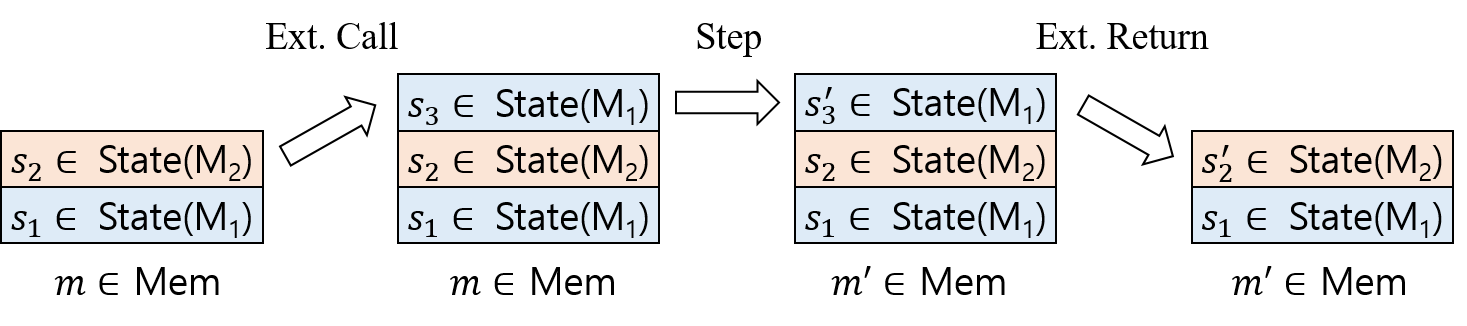
\includegraphics[width=0.9\linewidth]{images/intersem.png}
\caption{An execution of interaction semantics}
\label{fig:inter-sem}
\end{figure}

%% marshalling unmarshalling
%% marshalling the argument values into a list of values
%% setting the initial core states, unmarshalling the list of arguments.
%% at\_external: marshalling the argument values into a list of values
%% after\_external: unmarshalling the return value into
%% halted: marshalling the return value
%% corestep: use the underlying language semantics

Finally, note that the language semantics of C, assembly and
intermediate languages can be lifted to give a module semantics by
defining \texttt{corestep} to be the same as the execution step of the
language's semantics, and the other module operations to reflect the
calling conventions. Note also that all language-specific resources
(\ie other than the memory)
such as the register-file of assembly 
reside inside the module state, and thus are
duplicated at each invocation of a module.

%% One can lift a \cc{} language semantics into a core semantics by providing the interfaces:
%% Note that it is possible to define a core semantics using a mathematical specification.


\subsection{Open Simulation}
% \emph{core semantics}
The interaction semantics of \ccc{} gives a way to execute an
\emph{open} module $\module$ (\ie invoking external functions defined
outside $\module$) in isolation by providing a logical mechanism to
reflect possible interference from external function calls. More
specifically, the semantics provides two meta-level functions
$\mathtt{at\_external}$ and $\mathtt{after\_external}$. First,
$\mathtt{at\_external}~\stt = \mathtt{Some}~(f,\vec{v})$ denotes that
at language state $\stt$, an external function pointed to by a
function pointer $f$ is called with arguments $\vec{v}$. Second,
$\mathtt{after\_external}~r~\stt$ denotes the language state after the
external function call at $\stt$, assuming the call returned a value
$r$.
%% See \Cref{sec:overview-semantics:background} and \Cref{sec:main-semantics}
%% for more details about the interaction semantics.

%% $\mathtt{at\_external}$ detecting an external function call:
%% $\mathtt{at\_external}~\stt = \mathtt{Some}~(f,\vec{v})$ denotes that
%% at language state $\stt$, an external function pointed to by a
%% function pointer $f$ is called with arguments $\vec{v}$. Also, it
%% provides a meta-level function $\mathtt{after\_external}$ constructing the language state after
%% an external function call: $\mathtt{after\_external}~r~\stt$ denotes
%% the language state after the external function call at $\stt$, assuming
%% the call returned a value $r$. See \Cref{sec:main-semantics} for more details
%% about the interaction semantics.
%% \jeehoon{I don't think it's necessary to mention the word ``core semantics''. Why not just saying
%%   it's interaction semantics?}

Using interaction semantics, \ccc{} defines \emph{structured
  simulations} relating two open modules.
Here we briefly review the key ideas behind them,
which also occurred elsewhere, \eg in~\cite{pb,neis:pilsner,PLDI15}. \todo{check PLDI15}
First, unlike the closed simulations above,
structured simulations explicitly specify value and memory relations
(evolving over time) because values and memory are shared with external modules.
Specifically, such relations are defined using Kripke-style possible worlds,
called \emph{structured injections} \revision{(see \Cref{sec:overview-verification:injection} for more details)},
by giving $(i)$ a future world relation $\sqsupseteq$ for which
$w' \sqsupseteq w$ denotes that $w'$ is a future world of $w$;
and $(ii)$ value and memory relations at each world~$w$, denoted
$\mathtt{vrel}(w)$ and $\mathtt{mrel}(w)$.  Then, a
structured simulation $R$ gives a relation between machine
states at each world $w$, denoted $R(w)$, and should satisfy the
\emph{open} simulation property (simplified for presentation purposes) given in \Cref{fig:open-sim}.
\begin{figure}[t]
$
\begin{array}{@{}l@{}}
\texttt{ 1:}~\forall w,~ \forall (\memsrc,\memtgt)\in \mathtt{mrel}(w),~\forall \stsrc,\sttgt,~((\memsrc,\stsrc),(\memtgt,\sttgt))\in R(w)\implies{} \\[.5mm]
\texttt{ 2:}~\quad\textbf{match}~\mathtt{at\_external}~\stsrc~\textbf{with}\\[.5mm]
\texttt{ 3:}~\quad\mathtt{|}~\mathtt{Some}~(f_\src,\vec{v}_\src) \Rightarrow{}\\[1mm]
\texttt{ 4:}~\quad\quad \exists f_\tgt,\vec{v}_\tgt,~ \mathtt{at\_external}~\sttgt = \mathtt{Some}~(f_\tgt,\vec{v}_\tgt) \land{}\\[1mm]
\texttt{ 5:}~\quad\quad \fbox{$(f_\src,f_\tgt)\in \texttt{vrel}(w) \land (\vec{v}_\src,\vec{v}_\tgt) \in \overrightarrow{\texttt{vrel}(w)}$} \land{} \\[2mm]
\texttt{ 6:}~\quad\quad \dashbox{$\forall w' \sqsupseteq w,~\forall (\memsrc',\memtgt')\in\texttt{mrel}(w')$,}~ \dashbox{$\forall (r_\src,r_\tgt)\in \texttt{vrel}(w'),$}\\[2.5mm]
\texttt{ 7:}~\quad\quad ((\memsrc',\mathtt{after\_external}~r_\src~\stsrc),(\memtgt',\mathtt{after\_external}~r_\tgt~\sttgt))\in R(w') \\[.5mm]
\texttt{ 8:}~\quad\mathtt{|}~\mathtt{None} \Rightarrow{} \\[-.5mm]
\texttt{ 9:}~\quad\quad\forall e, \memsrc', \stsrc',~ (\memsrc, \stsrc) \estep{e} (\memsrc',\stsrc') \implies {}\\[.5mm]
\texttt{10:}~\quad\quad \exists \memtgt',\sttgt',~ (\memtgt,\sttgt) \estep{\tau}^{\raisebox{-1mm}{\scriptsize$\ast$}} \estep{e}\estep{\tau}^{\raisebox{-1mm}{\scriptsize$\ast$}} (\memtgt',\sttgt') \land{}\\[1mm]
\texttt{11:}~\quad\quad \fbox{$\exists w' \sqsupseteq w,~ (\memsrc',\memtgt') \in \mathrm{mrel}(w')$} \land {} \\[2.5mm]
\texttt{12:}~\quad\quad((\memsrc',\stsrc'), (\memtgt',\sttgt')) \in R(w')\\
\texttt{13:}~\quad\textbf{end}
\end{array}
$
\caption{Structured (or, open) simulations (simplified for presentation purposes)}
\label{fig:open-sim}
\end{figure}
% \jeehoon{In \texttt{at\_external} case, how about allowing the source to take silent steps?  Or
%   maybe we can remove silent steps also from the previous paragraph on CompCert's verification.}

Here the simulation involves rely-guarantee reasoning and is split
into two cases: one for interactions with external modules and the
other for internal steps (omitting two more cases for function start and end,
for presentation purposes). Specifically, given
any world $w$, related memories at $w$ and machine states related by
the simulation relation $R$ at $w$ (line~1), we check whether the
source state is invoking an external function or taking an internal
step (line~2). In the former case (line~3), the target state should
also be invoking an external function (line~4) and the invoked
functions and arguments should be related by the value relation at the
world~$w$ (line~5), which is a \fbox{guarantee condition} to the external modules.
Then we assume that the invoked external
functions proceed to a future world $w'$ yielding related memories and
related return values at $w'$ (line~6), which is a \dashbox{rely condition} from the external modules.
Under the assumption, the machine
states after the external calls should also be related by the
simulation relation $R$ at the future world $w'$ (line~7). In the
latter case (line~8), for any internal step from the source state
(line~9), there should be corresponding internal steps from the
target state (line~10).  Then the resulting memories after the steps
should be related at some future world $w'$ (line~11), which is a
\fbox{guarantee condition} to the external modules.  Finally, the
machine states after the steps should also be related by the
simulation relation $R$ at the future world $w'$ (line~12).

At high level, this simulation property specifies that internal
executions of the source and target modules should be related in
lockstep satisfying the guarantee conditions to the external modules,
assuming that the rely conditions from them hold after each external
function call.  Note that the rely and guarantee conditions on memory
(at lines 6 and 11) are matched and also those on values (at lines 5
and 6) will be matched if we include the omitted cases for function
start and end. This matching---in addition to the fact that the same
rely/guarantee conditions are used globally (\ie for verification of
every module)---is crucial for proving preservation of the simulation
property after linking modules because otherwise what one module
assumes about the other modules will not match with what the other
modules guarantee.

To use structured simulations for compiler verification, \ccc{} proves
the following three key properties, where we say a source module
$\module$ simulates a target module $\module'$ if there exists a
structured simulation that relates $\module$ and $\module'$:
\begin{itemize}
\item \textbf{(\emph{Vertical Compositionality})}
  If $\module$ simulates $\module'$, which simulates $\module''$,
  then $\module$ simulates~$\module''$.
\item \textbf{(\emph{Horizontal Compositionality})}
  If $\module_1$ and $\module_2$ simulate
     $\module'_1$ and $\module'_2$ respectively,
  then the linked source module  $\module_1 \llink \module_2$ simulates
  the linked target module $\module'_1 \llink \module'_2$.
\item \textbf{(\emph{Adequacy})}
  If $\module$ simulates $\module'$,
  then $\beh{\module} \supseteq \beh{\module'}$.
\end{itemize}






\subsection{Memory Relations of \cc{}}
\label{sec:overview-verification:injection:original}
%
\cc{}'s memory model consists of a finite set of blocks of finite size
and a pointer value (or, an address) is a pair $(b,o)$ of a block id $b$ and an offset $o$ inside it.
The memory identity imposes that the source and target memories are identical;
and the extension that the two memories contain identical block ids and
each target block extends the corresponding source block
with more space and any values in it at the end.

A memory injection injects a subset of the source blocks into target blocks
without overlap. More precisely, a (selected) whole source block is injected into a single target block
while allowing multiple source blocks to be injected into the same target block without overlap.
This injection map specifies the \emph{public} areas of the source and target memories and the correspondence between them.
In other words, the corresponding addresses by the injection map are treated as \emph{equivalent} (public) pointer values,
%% and therefore
so that at those corresponding addresses,
only equivalent%
\footnote{Technically speaking, \cc{} allow more undefined values in the source
  because it proves refinement rather than equivalence between the source and target programs.}
values (\ie equivalent non-pointer values or corresponding addresses) should be stored .
All the areas that are not on the injection map are considered as \emph{private} areas of the source and target memories.





%% \chapter{\;\;\;Theory of RUSC}
%% \label{chap:rusc}
%% \section{Problems with Open Simulation}
\label{sec:overview-verification:problems}
%% \myparagraph{Problems}
%
%   9051 /   2839 = 3.2 (id)
%  22124 /   8129 = 2.7 (ext)
%  23564 /   9128 = 2.6 (inj)
%
% Total
%  54739 /  20096 = 2.7  (pass)
% 152363 /  92029 = 1.65 (meta)
% 207102 / 112125 = 1.84 (whole)
%
%% Structured simulations of \ccc{} suffer from the problem that
%% verification using them is significantly more costly than that using
%% closed simulations of \cc{}: the Coq scripts for the verification of
%% all passes in \ccc{} is roughly \todo{2.7} times as large as that in
%% the original \cc{} in terms of lines of code~(LOC).
%% \jeehoon{How about reporting significant lines of code (SLOC)?}

As discussed in the introduction, verification using structured
simulations is significantly more costly than that using closed
simulations.  The reasons are twofold.

First, \revision{while closed simulations freely allow arbitrary memory relations---%
therefore \cc{} uses three different kinds of memory relations to simply proofs---%
%% ---thereby \cc{} uses three relations, \emph{memory identity, extension and injection}---
structured simulations only allow a single type of memory relations
called \emph{structured injections} due to horizontal compositionality.}
%
The reason is that, as discussed above,
%% in the background section,
allowing different memory relations would introduce
different rely/guarantee conditions
thereby breaking simulation after linking (\ie horizontal
compositionality) due to the mismatch between different rely/guarantee
conditions.
%% To see the reason, recall that, as we have seen in the
%% background section, the rely/guarantee conditions are determined by the
%% memory (and value) relations and the same rely/guarantee conditions
%% should be used globally to preserve simulations after linking
%% modules (\ie to prove horizontal compositionality).
%% Therefore allowing different memory relations for verifying
%% different modules would be problematic for proving horizontal
%% compositionality together with adequacy.

\revision{Second,
%% the notion of structured injection of \ccc{} is more complex than that of
%% \emph{memory injection} of \cc{} and, as far as we understand, such
%% complexity is needed for vertical compositionality.
%% It is well known that
proving vertical compositionality for \emph{open} simulations is in general
very technical and involved~\cite{ICFP19,neis:pilsner}. Indeed the
proof for structured simulations is about 5,000 SLOC in Coq.
Moreover, vertical compositionality also introduces unnecessary complexities
in structured simulations of \ccc{} such as \emph{effect annotations}
and \emph{closedness under restriction} \cite{stewart:ccc}.}
%% which makes correctness proofs of compiler passes more involved
%% (see \Cref{sec:overview-verification:injection} for discussion).}

To sum up, although it is quite straightforward to prove horizontal
compositionality and adequacy for a single relation (\ie with the same
rely/guarantee conditions), it is challenging to prove $(i)$ vertical
compositionality even for a single relation and $(ii)$ horizontal
compositionality between different relations (\ie with different
rely/guarantee conditions).

%\section{Refinement Under Self-related Contexts (RUSC)}
\section{RUSC}
\label{sec:overview-verification:solution}

%% \myparagraph{Our Solution at High Level}
%
Our solution is twofold. First, we develop a general and abstract
theory, called \emph{Refinement Under Self-related Contexts (RUSC)},
which is inspired by the standard notion of contextual refinement
\revision{and the notion of self-related context from \cite{stewart:ccc}
  (see \Cref{sec:related} for comparison).}
%\scc{}~\cite{?} (see \Sref{sec:related} for comparison).
Specifically, given a set of (arbitrary and independent)
relations each of which is horizontally compositional and adequate,
RUSC completes the relations by giving a super-relation (\ie
including all of them) that is horizontally and vertically
compositional and also adequate. Second, we prove that
our version of structured simulations, called \emph{open simulations},
with almost arbitrary memory relations
are horizontally compositional and adequate,
so that we can apply RUSC to open simulations with any chosen set of memory relations.

\myparagraph{Theory of RUSC}
%
RUSC can be defined abstractly for any linking algebra, which consists
of a set of modules, $\Module$, with a notion of behavior\footnote{Behaviors just need to be defined for closed programs.
  Technically, we can give undefined behavior (UB) to open modules.
%  For open modules, invoking an unknown function can be defined as undefined behavior (UB).
}, denoted
$\beh{p}$ for $p\in\Module$, a linking operation~$\llink$ between modules
that is associative%
\footnote{\revision{Commutativity does not hold for linking of \cc{} modules
    because changes in the order of global variables affect the initial memory after loading
    due to \cc{}'s deterministic memory allocation.}},
\revision{and the identity (\ie empty) module $\identity \in \Module$}:
\[
\begin{array}{c}
\llink: \Module \times \Module \rightarrow \Module \\
\forall p,q,r\in\Module,~p \llink (q \llink r) = (p \llink q) \llink r \\
\revision{\forall p \in\Module,~ \identity \llink p = p \llink \identity = p} \\
\end{array}
\]
Note that RUSC can be applied to interaction semantics because it
allows linking between arbitrary modules sharing the same notions
of value and memory (see \Cref{sec:overview-semantics:background} and \Cref{sec:main-semantics} for details).

To define RUSC, let $\rels$ be a set of module relations each of which is horizontally
compositional and adequate: for any $R \in \rels$ and $p,p',q,q'\in \Module$,
\[
\begin{array}{r@{}l@{\qquad}l}
(p,p'),(q,q')\in R &{}\implies (p \llink q, p' \llink q') \in R &\textrm{(\emph{HorComp})} \\
(p,p') \in R &{}\implies \beh{p} \supseteq \beh{p'} &\textrm{(\emph{Adequacy})} \\
\end{array}
\]
Then the RUSC relation for $\rels$, denoted $\rusc_{\rels}$, is defined as follows:
\[
\begin{array}{rcl}
p \rusc_{\rels} p' &\text{\emph{iff}}& \revision{\forall c_1, c_2 \in \self{\rels},~
\beh{c_{1} \llink p  \llink c_2} \supseteq \beh{c_{1} \llink p' \llink c_2}} \\
\self{\rels} & \defeq & \setof{ c \in \Module \suchthat \forall R \in \rels,~ (c,c) \in R }
\end{array}
\]
The definition is simple: $p$ is RUSC-related to $p'$ if the behaviors of $p'$ refine those of $p$ under
arbitrary contexts that are related to themselves by every relation in $\rels$.
% \jeehoon{From the definition of $p \rusc_{\rels} p'$, I think maybe it's easier to distinguish the
%   module type and the list-of-modules type... I know it's vague. Let's discuss offline.}

\begin{theorem}[Properties of RUSC]\label{thm:rusc} The RUSC relation $\rusc_\rels$ satisfies the following key properties.\\[.5mm]
$
\begin{array}{@{\quad}lrl}
 \text{(Inclusion)} &\forall R \in \rels,& R \subseteq {\rusc_\rels} \\[.5mm]
 \text{(Adequacy)} &\forall p,p'\in\Module,& p \rusc_{\rels} p' \implies \beh{p} \supseteq \beh{p'} \\[.5mm]
 \text{(VerComp)} &\forall p,p',p''\in\Module,& p \rusc_{\rels} p' \land p' \rusc_{\rels} p'' \implies p \rusc_{\rels} p'' \\[.5mm]
 \text{(HorComp)} &\forall p,p',q,q'\in \self{\rels},&   p \rusc_{\rels} p' \land  q \rusc_{\rels} q' \implies p \llink q \rusc_{\rels} p' \llink q' \\[.5mm]
 \revision{\text{(SelfComp)}} & \revision{\forall p,q \in \self{\rels},}& \revision{p \llink q \in \self{\rels}}
\end{array}
$
\end{theorem}
Note that horizontal compositionality holds only for self-related
modules, which, however, is not a big deal in practice as we will
discuss below.
\begin{proof}
The proof of the theorem is simple.  The
inclusion $R \subseteq {\rusc_\rels}$ trivially follows from the
horizontal compositionality and adequacy of $R$.  Adequacy of
$\rusc_\rels$ directly follows from the definition of $\rusc_\rels$ by
taking the empty context. Vertical compositionality (\ie transitivity)
of $\rusc_\rels$ holds trivially by definition.  Horizontal
compositionality, $p \llink q \rusc_{\rels} p' \llink q'$, is proven
in two steps using transitivity: $(i)$ $p \llink q \rusc_{\rels} p' \llink q$,
which follows from the definition of $p \rusc_{\rels} p'$ since $q\in\self{\rels}$,
and $(ii)$ $p' \llink q \rusc_{\rels} p' \llink q'$, which follows
similarly since $q \rusc_{\rels} q'$ and $p'\in\self{\rels}$.
%% ${R} \subseteq {\rusc_{\setofz{R}}}$ and
%% ${\rels} \subseteq {\rels'} \implies {\rusc_{\rels}} \subseteq {\rusc_{\rels'}}$
\revision{Finally, self-relatedness is closed under composition
because every relation in $\rels$ is horizontally compositional.}
\end{proof}

The reason why vertical compositionality is easily proven for RUSC
is that we essentially prove it for \emph{closed} programs by
closing an open module with contexts. Indeed, the technical
difficulties with vertical compositionality for open
simulations arise from the openness: it is difficult to set up a
setting properly with arbitrary future memories given after an external
function call.

The reason why horizontal compositionality holds between different
relations is interesting. Directly composing two simulations $(p,p') \in R_1$
and $(q,q') \in R_2$ with different relations $R_1$ and $R_2$
does not work in general. However, each simulation can be easily
extended with identical contexts because a pair of identical modules
usually respects any sensible relational principles. Therefore,
we have $(p \llink q ,p' \llink q) \in R_1$ and
$(p' \llink q ,p' \llink q') \in R_2$, which can be transitively composed
by vertical compositionality just as discussed above.
%% \jeehoon{I think we can say our horizontal compositionality proof, not the entire RUSC, is inspired
%%   from \scc{}.}

To sum up, RUSC provides a general condition for composing
different relational proofs: each proof just needs to be compatible
with its context modules in terms of self-relatedness, not necessarily
with their relational proofs.
%% instead of their relational proofs.

%% \begin{figure}
%%   \centering
%%   \includegraphics[width=0.70\linewidth]{rusc.jpg}
%%   \caption{Proving compositional compiler correctness with RUSC
%%   }
%%   \label{fig:rusc}
%% \end{figure}

%% \todo{add a fig:
%%   small horizontal compositionality figure,
%%   say that compatibility of rely/guarantee conditions between two relations (no)
%%   say that compatibility of rely/guarantee condition vs. the context I linked with. (yes)
%% }

\myparagraph{Open Simulations}
%
%% \todo{talk about analysis}
%% Since we can obtain vertical and horizontal compositionality
%% using RUSC, we can use simpler simulation relations (with different
%% memory relations)---which we call \emph{open simulations}---than
%% structured simulations (with structured injections).
%% Basically, open simulations contain only the core mechanism of
%% structured simulation presented in \Cref{sec:overview-verification:background}
%% without unnecessary complications needed to prove vertical
%% compositionality.

\revision{Since we can obtain vertical and horizontal compositionality using RUSC,
we can use open simulations with almost arbitrary memory relations.}
More specifically, we prove that open simulations with
\emph{any} Kripke-style memory/value relation satisfying certain minimal
conditions (see \Cref{sec:main-verification:parameter} for details) are horizontally compositional
and adequate. Since the required conditions are so minimal, they are
satisfied by the three memory relations---memory identity, extension
and injection---and also by a more powerful relation,
called \emph{memory injection with module-local invariants}.
This new memory relation is needed to
verify a new pass we added, called \texttt{Unreadglob}, which
requires reasoning about module-local states enabled by \emph{static}
variables of C (see \Cref{sec:overview-modulelocal} for details).

%% (emphasize that RUSC allows different techniques for different passes.
%% Additionally, analysis passes and assumptions on global variables).
Note that unlike \cc{} 2.1 on which \ccc{} is based, \cc{} 3.5
implements a static analyzer performing value analysis, which is used by
several passes. In order to support independent modular verification of such analyzers,
we also parameterize open simulations with memory predicates---representing the
analysis results of such analyzers---and
prove their horizontal compositionality and adequacy (See \Cref{sec:main-verification} for details).

\myparagraph{Applications} In our paper, we use RUSC
% with open simulations
in two situations: compiler and program verification.
%% \jeehoon{On paragraph name: how about ``Applications''?  It sounds more general.}

First, we give an abstract example for compiler
verification.  Suppose our source program is written in three modules,
\texttt{a.c}, \texttt{b.c} and \texttt{c.asm}, and compiled via
multiple passes: $\texttt{a.c}\to\texttt{a.il1}\to\texttt{a.asm}$ and
$\texttt{b.c}\to\texttt{b.il2}\to\texttt{b.il3}\to\texttt{b.asm}$,
each of which is verified using a different relation as follows:
\[
\begin{array}{l}
  (\texttt{a.c},\texttt{a.il1}) \in R_1 \quad (\texttt{a.il1},\texttt{a.asm}) \in R_2 \\
  (\texttt{b.c},\texttt{b.il2}) \in R_3 \quad
  (\texttt{b.il2},\texttt{b.il3}) \in R_4 \quad
  (\texttt{b.il3},\texttt{b.asm}) \in R_5
\end{array}
\]
%
Then as long as the \emph{end modules}, \texttt{a.c}, \texttt{b.c}, \texttt{a.asm},
\texttt{b.asm}, \texttt{c.asm}, are self-related by the relations $R_1,\ldots,R_5$,
using RUSC we can obtain the following behavioral refinement:
\[
\beh{\texttt{a.c} \llink \texttt{b.c} \llink \texttt{c.asm}} \supseteq \beh{\texttt{a.asm} \llink \texttt{b.asm} \llink \texttt{c.asm}}
\]
The underlying reasoning is simple: for $\rels=\setof{R_1,\ldots,R_5}$, we get
\begin{itemize}
\item $\texttt{a.c} \rusc_\rels \texttt{a.asm}$ and $\texttt{b.c} \rusc_\rels \texttt{b.asm}$
  by Inclusion and VerComp of \Cref{thm:rusc};
\item $\texttt{c.asm} \rusc_\rels \texttt{c.asm}$ since
  %% $\texttt{c.asm} \in \self{\rels}$ and thus
  $(\texttt{c.asm},\texttt{c.asm}) \in R_1 \subseteq \rusc_\rels$
  by Inclusion of \Cref{thm:rusc};
  %% \jeehoon{I don't understand it..}
\item $\texttt{a.c} \llink \texttt{b.c} \llink \texttt{c.asm} \rusc_\rels \texttt{a.asm} \llink \texttt{b.asm} \llink \texttt{c.asm}$
  by HorComp of \Cref{thm:rusc};
\item $\beh{\texttt{a.c} \llink \texttt{b.c} \llink \texttt{c.asm}} \supseteq \beh{\texttt{a.asm} \llink \texttt{b.asm} \llink \texttt{c.asm}}$ by Adequacy of \Cref{thm:rusc}.
\end{itemize}
Note that we need to prove the self-relatedness only for the end
modules because we only link those, not the intermediate ones
like \texttt{a.il1}, \texttt{b.il2}, \texttt{c.il3}.
Moreover, proving self-relatedness by a relation is typically
straightforward as long as the relation is sensibly defined.  Indeed,
we could easily prove that \emph{all} Clight\footnote{Clight is taken
  as the source language in most verification projects using \cc{}
  such as VST~\cite{VST}, CertiKOS and even \ccc{}.
  However, we also prove behavioral refinement w.r.t. the C source language
  (see \Cref{sec:results}).
}
and assembly programs are
self-related by all the relations used by \ccm{}
(\ie open simulations with memory identity, extension,
and injection with or without module-local invariants).
%% \jeehoon{How about ``we could easily prove that \emph{all} C, Clight, ...''}

Second, we demonstrate, via small but interesting examples (see \Cref{sec:overview-modulelocal}),
% (see \Cref{sec:overview-modulelocal} and \Cref{sec:utod-verification}),
%% the possibility
that our framework can be used to verify program modules
against (open) mathematical specification modules, written in Coq's Gallina language.
In the above example, for instance, we can prove
\[
\begin{array}{c}
\texttt{a.spec} \rusc_\rels \texttt{a.c}\quad
\texttt{b.spec} \rusc_\rels \texttt{b.c}\quad
\texttt{c.spec} \rusc_\rels \texttt{c.asm}
\\
\texttt{abc.spec} \rusc_\rels \texttt{a.spec} \llink \texttt{b.spec} \llink \texttt{c.spec}
\end{array}
\]
and link them together with the compiler correctness results above to get
\[
\beh{\texttt{abc.spec}}
\supseteq %% \rusc_\rels
%% \texttt{a.spec} \llink \texttt{b.spec} \llink \texttt{c.spec}
%% \rusc_\rels
\beh{\texttt{a.asm} \llink \texttt{b.asm} \llink \texttt{c.asm}}
\]
as long as the mathematical specification modules \texttt{a.spec},
\texttt{b.spec}, \texttt{c.spec}, \texttt{abc.spec} are in $\self{\rels}$,
which is usually straightforward to prove.

\myparagraph{Comparison to Contextual Refinement}
%
As one can easily see, RUSC refines the standard notion of contextual
refinement: instead of quantifying over \emph{all} contexts, RUSC
quantifies over only \emph{self-related} contexts. The main difference
is that RUSC gives the notion of well-behaved context w.r.t. a given
set of program relations (\ie reasoning principles) in terms of
contexts self-related by them.  This is particularly useful when not
all contexts are well behaved.  For example, in the interaction
semantics allowing mathematical specification modules as above, one can
easily write a specification module that arbitrarily changes the whole
memory including other modules' private memory. Under the presence of
such ill-behaved contexts, the contextual refinement will end up being too
strong preventing any reasoning about private memory such as
functions' stack frames. On the other hand, RUSC w.r.t. a set of
sensible relations will rule out such bad contexts and give us a sensible (better) relation.
%% even in the presence of such ill-behaved contexts.

%% \todo{Revise:
%% To sum up, the theory of RUSC tells that different relational proofs
%% well compose as long as the contexts of your interest are self-related
%% by the proof techniques of your interest.
%% }

%% because RUSC quantifies over only well-behaved contexts (\ie self-related ones
%% w.r.t. the given set of relations).

%% \hide{
%% We first review \cc{}'s correctness statement and its verification
%% method (\Cef{sec:background:cc}), and then how \ccc{} extends \cc{}
%% to allow multi-language programs (\ie programs composed of modules written in
%% different languages including C, assembly and \cc{}'s intermediate languages) (\Cref{sec:background:ccc}).
%% %% \ccc{} generalizes them to handle interactions between modules written in different
%% %% languages (\Cref{sec:background:ccc}).
%% In addition, we review key semantic techniques used for verification of CompCert.
%% %% called undefined behavior and logical memory
%% (\Cref{sec:background:ub}).
%% }




%%% Local Variables:
%%% mode: latex
%%% TeX-master: "main"
%%% End:


%% \chapter{\;\;\;Application: CompCertM}
%% \label{chap:compiler}
%% %% \chapter{\;\;\;\;Compiler Verification: CompCertM} %%이러면 (toc 말고 본문에서) 넘침
\chapter{\;\;\;\;Compiler Verification}
\label{sec:compiler}

\section{Background}
\label{sec:compiler:background}

\subsection{A Brief Introduction on CompCert}

\myparagraph{Undefined Behavior}



\section{Problems}
\label{sec:compiler:problems}

The problems with the interaction semantics of \ccc{} are that it does
not satisfy two adequacy properties. First, the adequacy w.r.t. C says
that for any C modules $M_1,\ldots,M_n$, the behaviors of the linked
program according to interaction semantics $\beh{M_1 \llink
  \ldots \llink M_n}$ should \emph{be included in} those according to the
physical semantics $\beh{M_1 \plink \ldots\plink M_n}$.  The reason for
failure was quite simple and we could easily fix it: unlike \ccc{}, we allow passing
the \texttt{undef} value to an external module since the C semantics
does so, while we turn ill-typed values into \texttt{undef} when they
are passed to an external module.

Second, the failure of the adequacy w.r.t. assembly is more serious.
Adequacy says that for any assembly modules $M_1,\ldots,M_n$,
the behaviors of the linked program according to interaction
semantics $\beh{M_1 \llink \ldots \llink M_n}$ should \emph{include}
those according to the physical semantics $\beh{M_1 \plink \ldots\plink M_n}$.
Note that the direction is opposite since assembly is the target language.
As discussed before, the reason for failure is that
the interaction semantics of \ccc{} does not have a mechanism to detect
illegal interference and make it undefined behavior~(UB).

\section{Solution}
\label{sec:compiler:solution}

We identify the sources of inadequacy w.r.t. assembly as violations of
three assumptions made by standard compilers: two on the registers and one on the stack.
We discuss why they 
cause problems with counterexamples and show how to semantically
handle them without changing the underlying language semantics.

\subsection{Assumptions on the Registers}
\label{sec:overview-semantics-register}
%
The two problematic assumptions on the registers are that
an invoked assembly function $(i)$ should
preserve the initial values of the callee-save registers, and $(ii)$
should not access the memory via the leftover pointer values remaining
in those registers that are not involved in passing meaningful information to the callee,
which we henceforth call \emph{\nip{}} registers.
%% in those registers, which we call \emph{non-passing} registers,
%% that are not involved in passing information to the callee.
%% the \emph{non-passing} registers (\ie those registers not involved
%% in passing information to the callee).
%% We discuss these two conventions together because it is nontrivial to find a
%% single model that enforces both conventions at the same time.
%% \jeehoon{I don't understand the last sentence..}
%% \jeehoon{``\nip{}'': how about ``opaque''?}

\begin{figure}[t]
\fbox{\begin{minipage}{.9pc}\mbox{}\\[15.25mm](a)\\[13.45mm]\mbox{}\end{minipage}}
\hspace*{-2.7mm}
\begin{minipage}{0.70\textwidth}
\begin{Verbatim}[frame=single]
int main()   {          main:
  int* x = malloc(8);     ...
  x[0] = 0;               *(%rbx) = 0;
  x[1] = 1;               *(%rbx + 4) = 1;
  f();               -->  f();
  out(x[0]);              out(*(%rbx));
  ...                     ...
}
\end{Verbatim}
\end{minipage}
$\mbox{}~\mathlarger{\mathlarger{\mathlarger{\mathlarger{\mathlarger{\llink}}}}}~\mbox{}$
\\
\vspace{3mm}
\\
\fbox{\begin{minipage}{.9pc}\mbox{}\\[10.50mm](b)\\[8.70mm]\mbox{}\end{minipage}}
\hspace*{-2.7mm}
\begin{minipage}{0.33\textwidth}
\begin{Verbatim}[frame=single]
f:
  if (g(%rbx))
    %rbx = %rbx + 4;
  else
    *(%rbx) = 1;

\end{Verbatim}
\end{minipage}
\caption{A counterexample showing the problem with the assumptions on the registers}
\label{fig:reg-convention}
\end{figure}

\myparagraph{Counterexamples}
%
The example in \Cref{fig:reg-convention} shows how violations of the two
assumptions can invalidate correct compiler translations.
%% \jeehoon{I think counterexample should go to the problems section.}
%
The code in the left box~(a) shows a standard translation of C code into assembly
(written in pseudocode) performed by mainstream compilers like GCC and LLVM, where the accesses to
the array \texttt{x} are translated into accesses via the register
\texttt{\%rbx} assuming that \texttt{\%rbx} is set to contain the
address of \texttt{x}. An important point here is that the compiler
assumes that $(i)$ the value of \texttt{\%rbx} is unchanged across
the function call \texttt{f()} since it is a callee-save register,
and also $(ii)$ the values in the array pointed to by \texttt{\%rbx} are
unchanged across \texttt{f()} since the array's addresses do not escape
except via \nip{} registers like \texttt{\%rbx}.
Therefore, the compiler expects that \texttt{out(*(\%rbx))} in the target code
correctly outputs \texttt{0}.

The right box~(b) presents an example of handwritten assembly
(written in pseudocode) for function \texttt{f} that violates the
above two assumptions of the compiler. The code either increments
\texttt{\%rbx} by \texttt{4} or writes \texttt{1} to \texttt{*(\%rbx)}
depending on the result of call to \texttt{g}.  Now if we link the assembly
code in (a) and that in (b) together, one can easily see that
\texttt{out(*(\%rbx))} incorrectly outputs~\texttt{1} instead
of \texttt{0} in either case: in the former case, \texttt{\%rbx}
points to the second element of the array~\texttt{x}, which contains
\texttt{1}; in the latter case, the value of \texttt{*(\%rbx)} is
directly updated to \texttt{1}. Therefore, it makes sense to
define those illegal behaviors of (b) as undefined behavior~(UB).

\myparagraph{Our Model}
\label{sec:compiler:solution:model}
%
We present our model making the illegal behaviors UBs
in stages, explaining at each stage why naive models do not work.
%% \jeehoon{What's the difference between ``stage'' and ``state''?}
%% \jeehoon{We have ``Our Solution'' paragraph inside ``Our Solution'' section. How about moving
%%   counterexample to the problems section, and giving a paragraph to each stage?}

First, in order to enforce the preservation of callee-save register
values, we store the initial values of the callee-save registers at
the \texttt{init-core} step of assembly modules; and check, at the
\texttt{halted} step, whether the final values of those registers are
equal to the stored initial values and if not, raise UB.  Here, the
question is, when a new core with a fresh register file is pushed into the core stack,
what values should be set as initial values of the \nip{}
registers including all of the callee-save registers.  Since the
registers may contain arbitrary values in the physical assembly
semantics, a natural choice would be to initially set them to contain
the \texttt{undef} value, which is an abstract value representing all
possible values. Indeed, this is the choice of \ccc{}.  However, there
is a serious problem. Since, for instance, \texttt{undef + 4} results
in \texttt{undef}, checking whether the final values of callee-save
registers are equal to the initial values, \ie \texttt{undef}, is
not sufficient. Specifically, the assembly code in (b) above
does not raise UB in this new semantics in case \texttt{g(\%rbx)} returns \texttt{1}
because the initial and final values of \texttt{\%rbx}
are both \texttt{undef} and thus equal
even though the callee-save register \texttt{\%rbx} is incremented
by \texttt{4} in the physical semantics.

Second, another natural solution would be to initially set the
\nip{} registers to nondeterministically contain arbitrary
values including \texttt{undef}. Though this model is more flexible,
it still has a problem. For instance, in the above example, to
simulate the physical behaviors of the assembly function \texttt{f} in
interaction semantics, one can set the initial value of \texttt{\%rbx} to
be either $(i)$ \texttt{undef} (\ie a more abstract value than the physical one), or
$(ii)$ a pointer to the array \texttt{x} (\ie a value equivalent to the physical one):
other values cannot be used since they are not refined by the value of \texttt{\%rbx} in the target,
which is required since the value is passed to an unknown function~\texttt{g}.
In the former case, if
\texttt{g(\%rbx)} returns \texttt{1}, we have the same problem with
callee-save checking as shown above.  In the latter case, if
\texttt{g(\%rbx)} returns \texttt{0}, the function \texttt{f}
successfully updates the array~\texttt{x} thereby invaliding the
translation in (a) as illustrated above.

We solve this problem by further revising the second model:
nondeterministically allocating an arbitrary number of \emph{junk
  blocks} (\ie blocks of size zero) and then initializing the
\nip{} registers with arbitrary non-pointer values or
\emph{junk pointers} (\ie pointers to the junk blocks).  Then we can
simulate the physical behaviors by initializing each register $r$
$(i)$ with the same non-pointer value if the physical value of $r$ is
a non-pointer value; and $(ii)$ otherwise with a fresh junk pointer.
The high-level idea is that, like \texttt{undef}, a junk pointer is
more abstract (\ie causing more UBs) than any pointer but, unlike
\texttt{undef}, sufficiently distinguishable. For instance,
in the previous example, if \texttt{g(\%rbx)} returns \texttt{1},
the initial and final values of \texttt{\%rbx} (\ie $p$ and $p+4$ for a junk pointer $p$)
are distinguished thereby raising UB by the callee-save checking;
if \texttt{g(\%rbx)} returns \texttt{0},
the memory access \texttt{*(\%rbx) = 1} raises UB because \texttt{\%rbx}
points to a junk block of size zero.

Finally, note that introducing nondeterminism as above is not a
showstopper thanks to the mixed simulation, as discussed in
\Cref{sec:overview-verification:mixedsim}: we can do forward
simulation everywhere except for the \texttt{init\_core} step of
assembly modules, where we should do backward simulation.

\subsection{Assumptions on the Stack}
\label{sec:overview-semantics-memory}
%
The problematic assumption on the stack is that the
\emph{outgoing arguments area} of a caller's stack (\ie where overflowing function
arguments are stored) should be fully \emph{owned} by the callee. In
other words, the callee can assume that the arguments area is never
modified by others unless its addresses are revealed to the public by
the callee itself.

\begin{figure}[t]
\fbox{\begin{minipage}{.9pc}\mbox{}\\[10.45mm](a)\\[8.65mm]\mbox{}\end{minipage}}
\hspace*{-1.9mm}
\begin{minipage}{0.255\textwidth}
  \begin{Verbatim}[frame=single]
main:
  ...  
  leak = %rsp;
  f(..., 0);
g:
  *leak = 1;
  \end{Verbatim}
\end{minipage}
$\mbox{}~\mathlarger{\mathlarger{\mathlarger{\mathlarger{\mathlarger{\llink}}}}}~\mbox{}$
\fbox{\begin{minipage}{.9pc}\mbox{}\\[10.45mm](b)\\[8.65mm]\mbox{}\end{minipage}}
\hspace*{-1.9mm}
\begin{minipage}{0.695\textwidth}
  \begin{Verbatim}[frame=single]
void f(..., int64_t x)       f:
{                              ...
  out(x);                      out(*(%rax));
  g();                  -->    g();
  out(x);                      out(*(%rax));
}                              ...
  \end{Verbatim}
\end{minipage}
\\[1mm]
\fbox{\begin{minipage}{.9pc}\mbox{}\\[15.90mm](c)\\[15.10mm]\mbox{}\end{minipage}}
\hspace*{-2.7mm}
\begin{minipage}{.95\textwidth}
\fbox{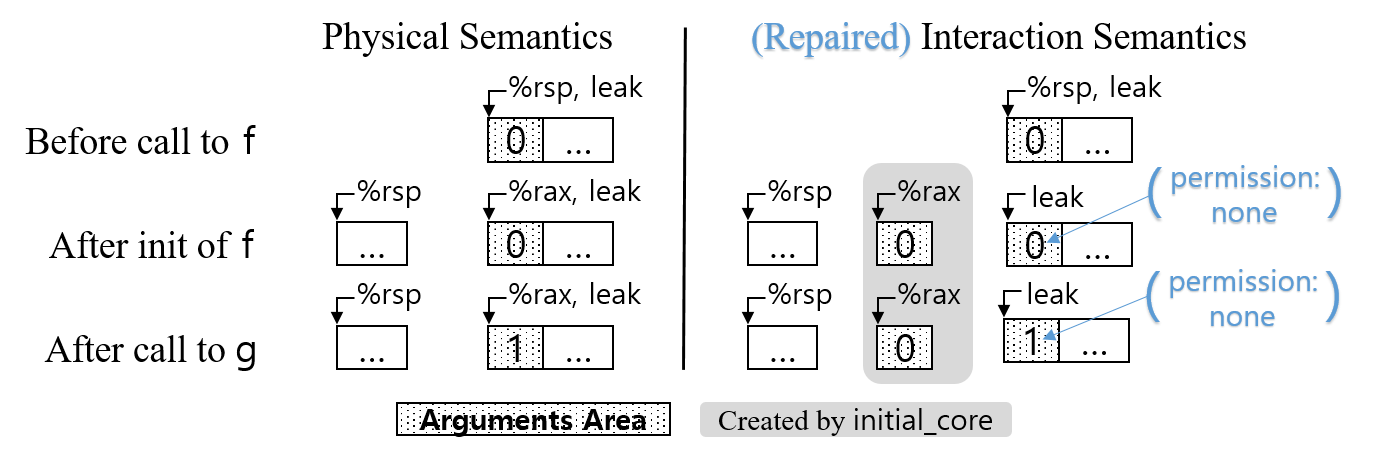
\includegraphics[width=.983\textwidth]{images/ex-stack.png}}
\end{minipage}
%% \fbox{\begin{minipage}{.8pc}\mbox{}\\[4.53mm](c)\\[3.73mm]\mbox{}\end{minipage}}
%% \hspace*{-1.9mm}
%% \begin{minipage}{.95\textwidth}
%%   \begin{Verbatim}[frame=single]
%%                      Physical Semantics         Interaction Semantics
%%                             %rsp           |                  %rsp       
%% Before call to f:           [=0=| ... ]    |                  [=0=| ... ]
%%                     %rsp    %rax           |    %rsp    %rax             
%%  After init of f:   [ ... ] [=0=| ... ]    |    [ ... ] [=0=] [=0=| ... ]
%%                     %rsp    %rax           |    %rsp    %rax             
%%  After call to g:   [ ... ] [=1=| ... ]    |    [ ... ] [=0=] [=1=| ... ]
%%   \end{Verbatim}
%% \end{minipage}
\caption{A counterexample showing the problem with the assumption on the stack}
\label{fig:stack-convention}
\end{figure}

\myparagraph{Counterexamples}
%
The example in \Cref{fig:stack-convention} shows how violations of the assumption
can invalidate correct compiler translations.
%
The box~(a) shows handwritten assembly code implementing two functions
\texttt{main} and \texttt{g}; the box~(b) shows a standard translation
of C code into assembly essentially performed by \texttt{gcc -O0}; and
the left-hand side (LHS) of the box~(c) depicts the shape of the stack
during execution in the physical semantics.
The function \texttt{main} stores the address of the
outgoing arguments area (\ie \texttt{\%rsp} as depicted in LHS of (c))
in the global variable \texttt{leak} and invokes the function
\texttt{f}, where the last argument \texttt{0} is stored in the
arguments area of the stack. Then the function \texttt{f} makes three
function calls, \texttt{out(x)}, \texttt{g()} and \texttt{out(x)},
where the argument \texttt{x} is directly read from the arguments area
pointed to by \texttt{\%rax} in the assembly, as depicted in LHS of
(c), and \texttt{out(x)} outputs the read value.  Finally, the
function \texttt{g} updates the arguments area pointed to by
\texttt{leak} with~\texttt{1}, as depicted in LHS of (c), between the
two function calls \texttt{out(x)}.

An important point here is that the compiler assumes that the
arguments area (\ie \texttt{\%rax}) is unchanged across the
function call \texttt{g()} since it is fully owned by \texttt{f}.
Therefore, the compiler expects that both calls
\texttt{out(*(\%rax))} in the target code correctly output
\texttt{0}. However, since the function \texttt{g} updates the
arguments area with \texttt{1} via \texttt{leak}, the two calls
incorrectly output \texttt{0} and~\texttt{1}.
We confirmed this incorrectness by
compiling \texttt{f} with \texttt{gcc -O2}, which
eliminates the second load \texttt{*(\%rax)} by propagating
the result of the first load across \texttt{g()}
thereby outputting \texttt{0} twice.

\myparagraph{Our Model}
%
In order to solve the problem, we have to distinguish accesses to the
arguments area via the caller from those via the callee and define the
former as UB. Though making such distinction is difficult in the
physical semantics, fortunately it is already made in interaction
semantics due to the language-independent design. For example, consider
the interaction semantics of the above example, depicted in the
right-hand-side (RHS) of \Cref{fig:stack-convention}~(c).  The
difference is that when the assembly function \texttt{f} is invoked,
the initialization process (\ie \texttt{init\_core}) of the module
semantics newly constructs the arguments area of the stack from the
given logical arguments in order to make an environment needed to
execute the assembly function \texttt{f}. This is essentially needed
because the caller may not be an assembly module so that it may not
have its own stack at all.  Then the callee sees the new arguments
area created by \texttt{init\_core} while the caller (in assembly)
sees the original arguments area.

Although the original interaction semantics does not prevent access to
the arguments area via the caller, we can easily fix it.
%% Now we can easily repair the original interaction semantics to make
%% those accesses to the arguments area via the caller as UB during the
%% lifetime of the callee.
We simply $(i)$ turn off the access
permission of the original arguments area in the \texttt{at\_external}
step of the caller module, and $(ii)$ turn it back on in the
\texttt{after\_external} step. Note that the notion of permission
%% is already an existing feature of
already exists in the \cc{} semantics, so that we do not
need to strengthen it. In the above example again,
the update by \texttt{g} will raise UB since the original argument area pointed
to by \texttt{leak} has no access permission.


\subsection{Mixed Simulation}
\label{sec:overview-verification:mixedsim}

While the target language of \cc{} is deterministic (more precisely,
the source is receptive and the target is determinate) thereby mostly
using forward simulations, the repaired interaction semantics of
\ccm{} is inherently nondeterministic to handle illegal interference from assembly modules
%% enforce the assembly calling conventions
(\Cref{sec:compiler:solution:model}) thus preventing the
use of forward simulation.
%% While it is theoretically possible to convert the \cc{}
%% verification from forward to backward simulations, it would incur a
%% significant cost since a compiler pass typically compiles a single
%% instruction in the source down to several instructions in the target.
%% %% due to the nature of source and target languages and the size of verification.
%% For this reason, determinism
%% has been considered ``instrumental for the simulation proofs of the compiler passes and its absence
%% is a show stopper''~\cite{besson:intptr}.
% Extending \cc{}'s semantics with such nondeterministic features can potentially cause significant
% overhead, as it invalidates forward simulation and enforces one to use backward simulation, which
% effectively means one should re-establish simulation proof from the scratch.  In literature, it is
% even said that

In order to recover the ability to use forward simulation in the occasional presence of nondeterminism,
we adopt the idea of \emph{mixed (forward-backward) simulation} from \cite{neis:pilsner}.
%% To embrace nondeterminism with low verification cost, we develop more general simulations, called
%% \emph{mixed simulations}, that (mostly) allow forward reasoning in the (occasional) presence of
%% nondeterminism.
The key observation is that
the requirement for using forward simulations (\ie determinism of the target) is a per-state property,
not a per-language property: as long as a particular target machine state is \emph{locally deterministic} (\ie its next state is unique),
one can do forward simulation at that state.
%% conversion from backward to forward simulations
%% requires only the current target \emph{machine state}, not the entire target \emph{language}, to be
%% deterministic.
Based on this observation, mixed simulations selectively allow forward
simulation when the target is locally deterministic, in addition to
the default backward simulation.
%% for each pair of related machine states, we allow the verifier to
%% \emph{choose} to perform either forward or backward reasoning, requiring that forward reasoning is
%% used only for locally deterministic target machine states.
%
Specifically, we say that a relation $R$ is a (closed) mixed simulation if
for all $(\mssrc, \mstgt) \in R$,
%% \makebox[\linewidth]{\makebox[1.2\linewidth]{
%% \begin{minipage}{1.2\linewidth}
\begin{enumerate}
\item
  $\forall e, \mstgt',~ \mstgt \estep{e} \mstgt' \implies {} $ \\
  $ \exists \mssrc',~ \mssrc \estep{\tau}^{\raisebox{-1mm}{\scriptsize$\ast$}} \estep{e}\estep{\tau}^{\raisebox{-1mm}{\scriptsize$\ast$}} \mssrc' \land (\mssrc', \mstgt') \in R$; or
\item
  $\forall e, \mssrc',~ \mssrc \estep{e} \mssrc' \implies {} $ \\
  $ \exists \mstgt',~ \mstgt \eustep{\tau}^{\raisebox{-1mm}{\scriptsize$\ast$}} \eustep{e}\eustep{\tau}^{\raisebox{-1mm}{\scriptsize$\ast$}} \mstgt' \land (\mssrc', \mstgt') \in R$\\
\end{enumerate}
%% \end{minipage}
%% }}
where $\ms \eustep{e} \ms'$ denotes that $\ms$ is locally deterministic and $\ms \estep{e} \ms'$.

\Cref{fig:mixedsim} visualizes this formulation of mixed simulation, where
%% presents an example of mixed simulations, where $R$ is a simulation relation; red and blue circle represent source and
%% target machine states, respectively;
solid and dotted arrows represent universally and existentially
quantified steps, respectively, and double circles represent locally
deterministic target states. In this figure,
since the first three target machine states are deterministic,
we can do forward simulation as shown in the figure;
then, since the following target state is nondeterministic,
we should do backward simulation as shown in the figure.
%% the first three target machine states are deterministic.  The
%% first three target steps are deterministic and reasoned in a forward manner (from source to target),
%% and the last target step is nondeterministic and reasoned in a backward manner (from target to
%% source).  Later, those part of simulations that are reasoned in a forward manner is converted to
%% backward reasoning, thereby proving backward simulation and thus behavior refinement.

Note that the repaired interaction semantics is nondeterministic only
at the initial step of a module invocation, so that we can do
forward simulation everywhere else using mixed simulations.

In order to support \cc{}'s condition for forward simulation,
we also add the following to the above formulation of mixed simulation:
\begin{enumerate}[resume]
\item or, $\mssrc$ is receptive and\\
  $\forall e, \mssrc',~ \mssrc \estep{e} \mssrc' \implies {} $ \\
  $ \exists \mstgt',~ \mstgt \exstep{\tau}^{\raisebox{-1mm}{\scriptsize$\ast$}} \exstep{e}\exstep{\tau}^{\raisebox{-1mm}{\scriptsize$\ast$}} \mstgt' \land (\mssrc', \mstgt') \in R$\\
  where $\ms \exstep{e} \ms'$ denotes that $\ms$ is locally determinate and $\ms \estep{e} \ms'$.
\end{enumerate}
Also we apply this mechanism of mixed simulation to our open simulations.

\begin{figure}[t]%% {0.43\textwidth}
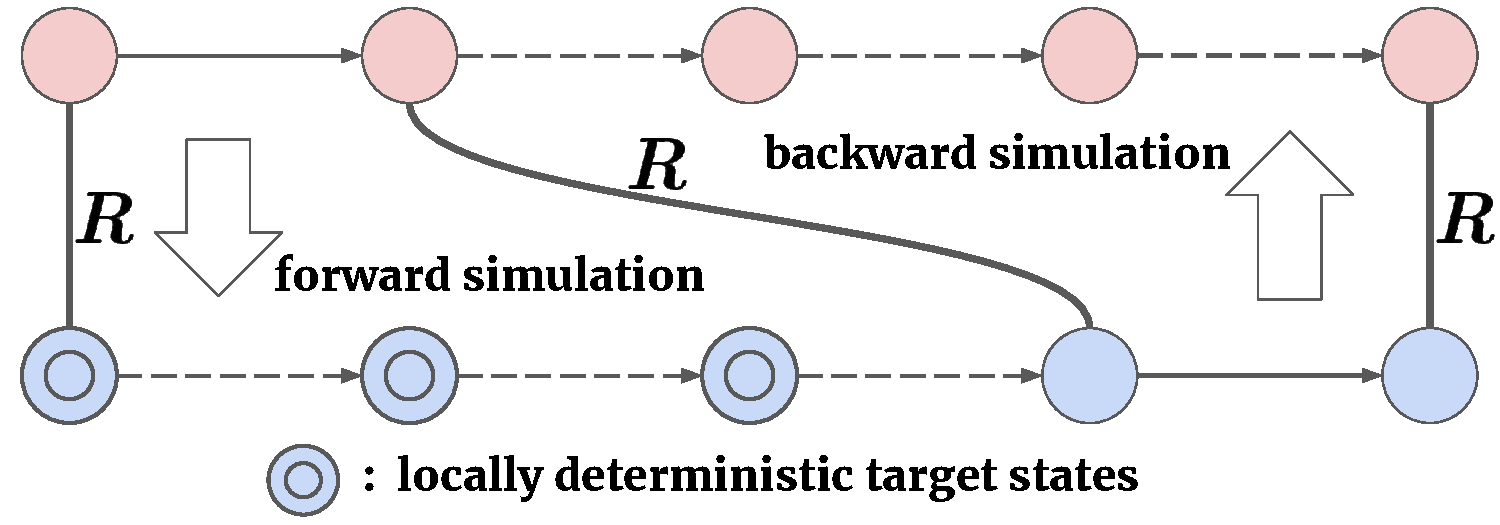
\includegraphics[width=0.7\textwidth]{images/mixed-sim-bold.pdf}
%% 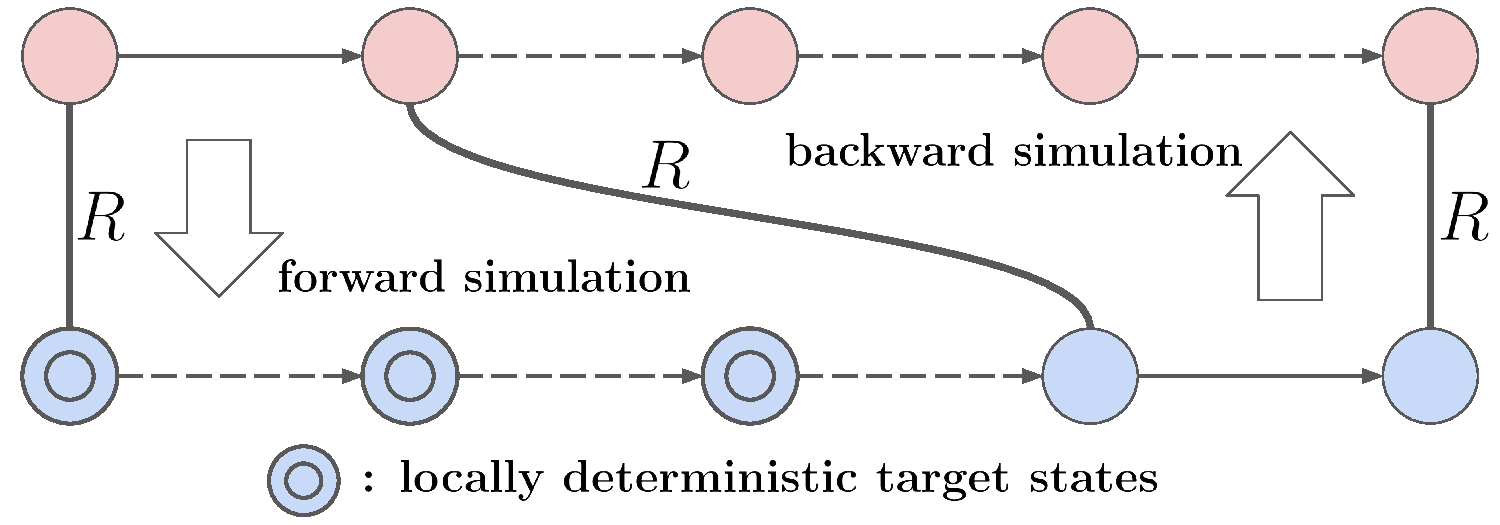
\includegraphics[width=0.7\textwidth]{images/mixed-sim.pdf}
\caption{A visualized example of mixed simulations}
\label{fig:mixedsim}
\end{figure}

\section{CompCertM}
\label{sec:compiler:compcertm}

Based on the theories we presented so far, we develop \ccm{}, an extension of \cc{} with the
repaired interaction semantics and open simulations to support multi-language linking.  We state
\ccm{}'s compositional correctness results (\Cref{sec:results:compiler}) and evaluate its
verification efforts (\Cref{sec:results:evaluation}).  \ccm{} currently supports the x86 backend only.
We do not currently see any technical problem with supporting other architectures.

\subsection{Compositional Correctness}
\label{sec:results:compiler}

\ccm{} uses open simulations with three parameters:
memory relations, symbol relations and memory predicates
(see \Cref{sec:main-verification:opensim} for details).
It supports $(i)$ the memory relations discussed in \Cref{sec:overview-verification:injection}:
identity, extension and (enriched) injections with no or any given module-local invariant;
$(ii)$ two symbol relations: one for keeping identical symbols in the source and target
and the other for allowing elimination of global variables in the target (only allowed for memory injections), needed for \code{Unusedglob} and \code{Unreadglob};
$(iii)$ two memory predicates: one for no analysis and the other for the value analysis of \cc{}.

Let $\rels$ be the set of open simulations with all possible parameters.
To apply RUSC, we prove that the \ccm{} compiler $\mathcal{C}$ transforms the source module with
a series of passes that are independently verified using open simulations in $\rels$.
\begin{lemma}[Pass Correctness]\label{thm:results-passes}
  For any \textrm{Clight} module $S$ and \textrm{Asm} module $T$, if $\mathcal{C}(S) = T$, then
  there exist intermediate modules $M_0, M_1, \cdots, M_n$ such that:
  \begin{enumerate}
  \item $M_0 = S$ and $M_n = T$; and
  \item $\forall i \in [0,n),~ \exists R \in \rels,~ (M_i, M_{i+1}) \in R$~.
  \end{enumerate}
\end{lemma}

We also prove all \textrm{Clight} and \textrm{Asm} modules are self-related.
\begin{lemma}[Self-Relatedness]\label{thm:results-relatedness} For any \textrm{Clight} or \textrm{Asm}
  module $M$, we have $M \in \self{\rels}$.
\end{lemma}
\noindent
\revision{Note that
  since we define illegal interference from Asm
  (\ie causing different behaviors in the source and target) as undefined behaviors (UBs)
  as shown in \Cref{sec:compiler:solution},
  every Asm module can be self-related.}

From \Cref{thm:results-passes,thm:results-relatedness}, the RUSC relation for the compiler follows.
\begin{theorem} [Modular Correctness]\label{thm:results-modular}
  For any \textrm{Clight} module $S$ and \textrm{Asm} module $T$, if $\mathcal{C}(S) = T$:
  \[
    {S} \rusc_\rels {T} \quad\text{with}\quad S,T \in \self{\rels}~.
  \]
\end{theorem}

\noindent
This theorem provides a truly compositional correctness
thanks to the compositionality of RUSC (\Cref{thm:rusc}):
%% The fact that the source and target are related by RUSC
%% implies that they satisfy behavioral refinement by adequacy of RUSC, and moreover
the relation can be freely (\ie vertically or horizontally) composed with any verification using RUSC
including that against mathematical specifications.
As an example, the following compositional correctness follows.
\begin{corollary} [Compositional Correctness 1]\label{thm:results-compiler}
  Let $(S_1,T_1), \ldots, (S_n,T_n)$ be pairs of source and target modules.
  If each pair is either compiled (\ie $\mathcal{C}(S_i) = T_i$ with $S_i$ \textrm{Clight} and $T_i$ \textrm{Asm}), or a self-related context (\ie $S_i = T_i \in \self{\rels}$), then
  \[
    \beh{S_1 \llink \cdots \llink S_n} \supseteq \beh{T_1 \llink \cdots \llink T_n}~.
  \]
\end{corollary}
%
\noindent This correctness theorem is compositional in the sense that behavior is refined in the
presence of any self-related contexts such as arbitrary \textrm{Clight} and \textrm{Asm} modules
(\Cref{thm:results-relatedness}).





Note that \textrm{Clight}, not \textrm{\cc{} C}, is the source language in the above theorems.  One of the
reasons is that \textrm{Clight} is the source language for most verification frameworks based on
\cc{}, such as VST~\cite{VST}, \ccc{}, and \ccx{}.  More importantly, we found that
\textrm{\cc{} C} is incompatible with memory injections.  Specifically,
\textrm{\cc{} C} imposes a strict alignment requirement on memory blocks of size zero, which, however,
%% but the requirement
is not preserved by memory injections.
%% For this reason, we cannot achieve full horizontal compositionality
%% in the presence of both \textrm{\cc{} C} modules and compiler passes verified using memory injections.
In other words, \textrm{\cc{} C} modules are not always self-related by memory injections.\footnote{This problem
  would be solved if one strengthens memory injections with more strict alignment requirements.}

\myparagraph{Supporting \textrm{\cc{} C}}
However, we can still prove a compositional correctness (not modular correctness as in \Cref{thm:results-modular}) for \textrm{\cc{} C}
following \scc{}'s \emph{Level A} technique~\cite{kang:scc},
which exploits the fact that all \textrm{CompCert C} modules are transformed to \textrm{Clight} modules
by the same two passes.
Specifically, the first pass is verified using an open simulation with the memory identity
and the second pass with memory injections, as done in the original \cc{}.
Then the following lemma follows from horizontal compositionality and adequacy of
open simulations (with memory identity and injection) and transitivity of behavioral refinement.

\begin{lemma} [ClightGen Correctness]\label{thm:results-clightgen}
  Let $(S_1,T_1), \ldots, (S_n,T_n)$ be pairs of source and target modules.
  If each pair is either translated (\ie $\textrm{ClightGen}(S_i) = T_i$ with $S_i$ \textrm{\cc{} C} and $T_i$ \textrm{Clight}), or a self-related context (\ie $S_i = T_i \in \self{\rels}$), then
  \[
    \beh{S_1 \llink \cdots \llink S_n} \supseteq \beh{T_1 \llink \cdots \llink T_n}~.
  \]
\end{lemma}



By composing \Cref{thm:results-compiler}, \Cref{thm:results-clightgen} and \Cref{thm:results-relatedness}, we have the following theorem.
\begin{theorem} [Compositional Correctness 2]\label{thm:results-compiler2}
  Let $(S_1,T_1), \ldots, (S_n,T_n)$ be pairs of source and target modules.
  If each pair is either compiled (\ie $\mathcal{C}(S_i) = T_i$ with $S_i$ \textrm{\cc{} C} or \textrm{Clight} and $T_i$ \textrm{Asm}), or a self-related context (\ie $S_i = T_i \in \self{\rels}$), then
  \[
    \beh{S_1 \llink \cdots \llink S_n} \supseteq \beh{T_1 \llink \cdots \llink T_n}~.
  \]
\end{theorem}


\myparagraph{Adequacy w.r.t. Physical Semantics}


We show that the repaired interaction semantics is adequate w.r.t. the physical semantics of \cc{},
where the former uses the language-independent linking $\llink$ and the latter the syntactic linking $\plink$
concatenating modules of the same language.

We prove that the physical semantics refines the repaired interaction semantics for \textrm{Asm} modules
using a closed simulation of \cc{} with memory injections.
\begin{theorem}[Adequacy w.r.t. Assembly]\label{thm:results-adequacy-asm}
  Let $M_1, \cdots, M_n$ be \textrm{Asm} modules.  We have:
  \[   \beh{M_1 \llink \ldots \llink M_n} \supseteq  \beh{M_1 \plink \ldots \plink M_n} ~.\]
\end{theorem}
\noindent
\revision{This theorem allows us to carry verification results on the interaction semantics such as \Cref{thm:results-compiler2}
down to \cc{}'s Asm semantics with syntactic linking.}



Conversely, we prove that the repaired interaction semantics refines the physical semantics for \textrm{\cc{} C} modules
using a closed simulation of \cc{} with memory identity.
This result is useful because we want to allow separate compilation (of C modules) on the compiler side, and on the program verification side, we want to hide complexities from inter-module steps.
\begin{theorem}[Adequacy w.r.t C]\label{thm:results-adequacy-c}
  Let $M_1, \cdots, M_n$ be \textrm{\cc{} C} modules.  We have:
  \[  \beh{M_1 \plink \ldots \plink M_n} \supseteq \beh{M_1 \llink \ldots \llink M_n}  ~.\]
\end{theorem}


In some sense, the \Cref{thm:results-compiler2,thm:results-adequacy-asm,thm:results-adequacy-c} together forms a strong stress-test for a language-independent linking, and our results show strong evidence that our repaired interaction semantics is indeed adequate (in a literal sense).
Specifically, if one of the three desiderata is missing, it is trivial to find language-independent linking satisfying the others.
Without \Cref{thm:results-adequacy-asm}, one can define interaction semantics to always execute UB; then, the other theorems become trivial.
Without \Cref{thm:results-adequacy-c}, one can define the behavior of interaction semantics to an empty set.
Without \Cref{thm:results-compiler2}, one can define $\llink \defeq \plink$.

%% These results mean that the repaired interaction semantics does not give too few behaviors to assembly programs (e.g., missing physically observable behaviors), nor does it give too many behaviors to well-typed C programs (e.g., giving UB to them).


Interestingly, by composing \Cref{thm:results-compiler2,thm:results-adequacy-asm,thm:results-adequacy-c}, we obtain
the same separate compilation correctness result of \scc{}~\cite{kang:scc}:

\begin{corollary}[Separate Compilation Correctness]
  Let $S_1, \ldots, S_n$ be \textrm{\cc{} C} modules and $T_1, \ldots, T_n$ be \textrm{Asm} modules.
  If $\mathcal{C}(S_i) = T_i$ for each $i$, we have:
  \[
    \beh{S_1 \plink \cdots \plink S_n} \supseteq \beh{T_1 \plink \cdots \plink T_n}~.
  \]
\end{corollary}

\youngju{Just mention that \ccc{} does not satisfy upperbound, and explain it in appendix?}
\youngju{here? or appendix?: To this end, we have strengthened \cc{}'s type checker in a number of
  ways, ruling out trivially wrong (according to C standard) programs more than before.  We rule out
  (i) a program that contains an identifier that is not declared in the module (ii) ``return''
  (without value) statement used for non-void function (iii) ``return'' (with value) statement used
  for void function (iv) function arguments containing void type.  (v) has duplicate (function or
  global variable) identifiers (vi) A function argument with size bigger than INT\_MAX (\cc{}
  already aborts on such programs)}





\subsection{Evaluation of Verification Efforts}\label{sec:results:evaluation}

\begin{table}[t]
\footnotesize

\parbox{\linewidth}{
\caption{SLOC of \ccm{} and related works --- compared to its baseline \cc{}, respectively}
\begin{tabu}{@{}l@{\hspace{1.55pt}}|[1.25pt]@{\hspace{1.55pt}} c @{\hspace{1.55pt}}|@{\hspace{1.55pt}} c @{\hspace{1.55pt}}|@{\hspace{1.55pt}} c @{\hspace{1.55pt}}|[1.25pt]@{\hspace{1.55pt}} c @{\hspace{1.55pt}}|@{\hspace{1.55pt}} c @{\hspace{1.55pt}}|[1.25pt]@{\hspace{1.55pt}}}
Portion     & \shortstack{\cc{} \\ 3.5} & \ccr{} 3.5        & \ccm{} pack                                               & \shortstack{\cc{}\\ 2.1} & \ccc{} \\
\hline
Pass Proofs & 34,376    & 35,893 (+4.41\%)  & \newrevision{4,923(+14.32\%)}                                          & 21,215    & 52,140 (+145.77\%) \\
The Rest    & 85,617    & 87,965 (+2.74\%)  & \newrevision{25,558(+29.85\%)}  & 59,365    & 107,910 \hspace{.6mm} (+81.77\%) \\
Total       & 119,993   & 123,858 (+3.22\%) & \newrevision{30,481(+25.40\%)}                                         & 80,580    & 160,050 \hspace{.6mm} (+98.62\%) \\
\end{tabu}
\\
\begin{tabu}{@{}l@{\hspace{1.55pt}}|[1.25pt]@{\hspace{1.55pt}} c @{\hspace{1.55pt}}|@{\hspace{1.55pt}} c @{\hspace{1.55pt}}|[1.25pt]@{\hspace{1.55pt}}}
Portion     & \shortstack{\cc{} \\ 3.0} & \ccx{}             \\
\hline
Pass Proofs & 26,466    & 30,572 (+15.51\%)  \\
The Rest    & 82,312    & 121,532 (+47.65\%) \\
Total       & 108,778   & 152,104 (+39.83\%) \\
\end{tabu}
\label{table:evaluation-ours}
}

%% \parbox{\linewidth}{
%% \label{table:evaluation-ours}
%% }
    
\parbox{0.38\linewidth}{
\vspace{4mm}
\caption{\mbox{Breakdown of \ccm{} pack}}
\begin{tabu}{@{}l | l@{}}
Portion                          & SLOC                                                                                                     \\
\hline
\revision{Proofs about Intermodule Steps} & \newrevision{4,923}                                                                                                    \\
Interaction Semantics/Properties & 1,940                                                                                                    \\
Language Semantics/Properties    & 1,701                                                                                                    \\
Self Simulations                 & \newrevision{5,593}                                                                                                    \\
\cc{}  Metatheory Extension      & \newrevision{4,688}                                                                                                    \\
\ccm{} Metatheory                & \newrevision{7,656}                                                                                                    \\
Mixed Simulation                 & 1,090                                                                                                    \\
Adequacy w.r.t. Asm              & 2,890                                                                                                    \\
\end{tabu}
\label{table:evaluation-breakdown}
}
\hfill
\parbox{0.45\linewidth}{
\vspace{4mm}
\caption{SLOC of additional developments}
%% \begin{tabu}{@{}l @{\;} |[1.25pt] @{\;} r @{\;} | @{\;} r @{\;} | @{\;} r @{\;} | @{\;} r @{\;} | @{\;} r @{}}
%% Portion                          & \shortstack{\texttt{Unreadglob} \\ 3.5} & \shortstack{\texttt{Unreadglob} \\ pack} & \texttt{mutual-sum} & \texttt{utod} & \shortstack{Adequacy \\ w.r.t. C} \\
%% \hline
%% Pass Proofs                      & 1,842                   & 338                      & 3,088               & 361           & -             \\
%% The Rest                         & 260                     & 1,933                    & 2,707               & 424           & 4,044         \\
%% Total                            & 2,102                   & 2,271                    & 5,795               & 785           & 4,044         \\
%% \end{tabu}
\begin{tabu}{@{}l @{\;} |[1.25pt] @{\;} r @{\;} | @{\;} r @{\;} | @{\;} r @{\;} | @{\;} r @{\;} | @{\;} r @{}}
Portion                          & \shortstack{\texttt{Unreadglob} \\ 3.5} & \shortstack{\texttt{Unreadglob} \\ pack} & \shortstack{Adequacy \\ w.r.t. C} \\
\hline
Pass Proofs                      & 1,842                   & 338                      & -             \\
The Rest                         & 260                     & 1,933                    & 4,044         \\
Total                            & 2,102                   & 2,271                    & 4,044         \\
\end{tabu}
\label{table:evaluation-others}
}%
\end{table}

\youngju{There are two ``unreadglob'' columns, one for \cc{} and one for pack. Simplify it}
\youngju{How about reducing caption text size?}
\jeehoon{``Per-pass'', ``Metatheory'', and ``Total'' instead of ``Pass Proofs'', ``The Rest'', and ``Whole''}

To demonstrate that \ccm{} is lightweight,
we compare significant lines of code (SLOC) of \ccm{}, \ccc{}, and \ccx{} with
those of their baseline \cc{} versions 3.5, 2.1, and 3.0, respectively.
Overall, \ccm{} adds less code to \cc{} than \ccc{} and \ccx{} do,
and in particular significantly less code than \ccc{} for the proofs of compiler passes.%
\footnote{\revision{Note that \ccc{} allows horizontal compositionality between any intermediate languages (ILs)
  while \ccm{} only between Clight and Asm since self-relatedness is proven only for the two.
  Though practically unnecessary, supporting linking between arbitrary ILs in \ccm{} would increase SLOC to prove self-relatedness for the other ILs.}}
\newrevision{Also note that \ccr{} uses the enriched memory injections of \Cref{sec:overview-verification:injection:dynamic} instead of the original memory injections
in order to give reusable main lemmas for both closed and open simulations.
Since \ccr{}'s pass proofs are only 4.41\% larger than \cc{}'s, 
the overhead due to handling the private memory components of enriched memory injections is, roughly speaking, at most 4.41\%.}

\Cref{table:evaluation-ours} summarizes the comparison.
For each compiler (\ie each column),
the rows report SLOC for the proofs of all compiler passes (Pass Proofs),
the rest of the development (The Rest),
and their summation (Total).
Note that \ccm{} is split into \ccr{} and \ccm{} pack, for which the former is our refactoring
of \cc{} and the latter is an additional package to support multi-language linking.
We counted SLOC reported by
\code{coqwc}.\footnote{Concretely, we counted ``spec'' and ``proof'' lines reported by \code{coqwc}.
  Because we use a different criteria for line numbers, they are different from those reported in
  prior work~\cite{stewart:ccc,gu:dscal,wang:saccx}.}  When counting SLOC, we excluded the following
code for fair comparison: $(i)$ code for other architectures than x86 because all three projects support
only x86; $(ii)$ code for the parser and type checker introduced in later versions of \cc{}; and $(iii)$ code for \textrm{ClightGen}, which is not supported by both \ccx{} and
\ccc{}.  We also excluded \ccc{}'s legacy proofs for the original compiler correctness.  We used the
latest development branches for the three projects.\footnote{Development as of November 8, 2019, available at: \url{https://github.com/snu-sf/compcertr}, \url{https://github.com/snu-sf/compcertm}, \url{https://github.com/PrincetonUniversity/compcomp}, \url{https://github.com/DeepSpec/dsss17/tree/master/CAL}}








\Cref{table:evaluation-breakdown} analyzes the \newrevision{30,481} SLOC for \ccm{} pack.
\revision{The pass proofs consist of \newrevision{4,923} SLOC for reasoning about intermodule steps, which is
  sometimes nontrivial since they perform the logical instrumentation presented in \Cref{sec:compiler:solution}.
  Note that \ccr{} provides proofs for intramodule steps as main lemmas, which are reused in \ccm{}.
}
The rest consists of
1,940 SLOC for the repaired interaction semantics and its properties;
1,701 SLOC for properties of each language such as determinism and receptiveness;
5,576 SLOC for self-relatedness (\Cref{thm:results-relatedness});
4,687 SLOC for extending the metatheory of CompCert;
7,569 SLOC for open simulations and other metatheory for \ccm{};
1,090 SLOC for mixed simulation; and
2,890 SLOC for adequacy w.r.t. assembly (\Cref{thm:results-adequacy-asm}).

%% \Cref{table:evaluation-others} shows SLOC for the new optimization pass and the verification examples
%% given in the dissertation.  Note that \code{Unreadglob} 3.5 adds the optimization to \ccr{} proving closed simulation
%% and \code{Unreadglob} pack to \ccm{} proving open simulation, which reuses the proof of \code{Unreadglob} 3.5 for intramodule steps.
%% As the verification of \code{mutual-sum} and \code{utod} show, directly proving
%% open simulation between programs and specifications is costly. 
%% We believe that program logics like VST~\cite{VST} can be used to prove such simulation,
%% which could significantly reduce the verification cost.
\Cref{table:evaluation-others} shows SLOC for the new optimization pass.  Note that \code{Unreadglob} 3.5 adds the optimization to \ccr{} proving closed simulation
and \code{Unreadglob} pack to \ccm{} proving open simulation, which reuses the proof of \code{Unreadglob} 3.5 for intramodule steps.


\section{Formal Semantics}
\label{sec:compiler:semantics}
abc

\section{Formalization of Verification Techniques}
\label{sec:compiler:verification}
abc

\section{Related Work}
\label{sec:compiler:related}
abc


%% \chapter{\;\;\;Application: Program Verification}
%% \label{chap:program}
%% \chapter{\;\;\;\;Program Verification}
\label{sec:program}

\section{Background}
\label{sec:program:background}

\section{Problems}
\label{sec:program:problems}

\section{Solution}
\label{sec:program:solution}


%% \chapter{\;\;\;Conculsion}
%% \label{chap:concl}
%% \input{concl}

%% \appendix

%% \chapter{\;\;My Appendix}
%% \lipsum[1-3]

\bibliographystyle{abbrv}
\bibliography{references}

%% \begin{thebibliography}{00}
%% \addcontentsline{toc}{chapter}{\bibname}

%% % 영문저널의 경우
%%     \bibitem{ref1} B. Jeon and J. Jeong, ``Blocking artifacts
%%     reduction in image compression with block boundary discontiunity
%%     criterion,'' {\em IEEE Transactions on Circuits and Systems for
%%     Video Tech.}, vol. 8, no.3, pp. 345-357, June 1998.

%% % 영문학술대회의 경우
%%     \bibitem{ref2} W. G. Jeon and Y. S. Cho, ``An equalization
%%     technique for OFDM and MC-CDMA in a multipath fading channels,''
%%     in {\em Proceedings of IEEE Conference on Acoustics, Speech and
%%     Signal Processing}, Munich, Germany, May 1997. pp. 2529-2532.

%% % 국내저널의 경우
%%     \bibitem{ref3} 김남훈, 정영철, ``평탄한 통과대역 특성을 갖는
%%     새로운 구조의 광도 파로열 격자 라우터,'' {\em 전자공학회논문지},
%%     제35권 D편, 제3호, 56-62쪽, 1998년 3월.

%% % 국내학술대회의 경우
%%     \bibitem{ref4} 윤남국, 김수종, ``무선 센서 네트워크에서의 에너지
%%     효율적인 그라디언트 기반 라우팅 기법,'' {\em 한국정보과학회
%%     2006년 추계학술대회}, 제12권, 제2호, 2006년 10월. pp.
%%     1372-1374.

%% % 단행본의 경우
%%     \bibitem{ref5} C. Mead and L. Conway, {\em Introduction to VLSI
%%     Systems}, Addison-Wesley, Boston, 1994.

%% % URL
%%     \bibitem{ref6} The SolarMESH Network,
%%     http://owl.mcmater.ca/solarmesh

%% % Technical Report의 경우
%%     \bibitem{ref7} K. E. Elliott and C. M. Greene, ``A local adaptive
%%     protocol,'' Argonne National Laboratory, Argonne, France,
%%     Technical Report 916-1010-BB, 1997.

%% % 학위논문의 경우
%%     \bibitem{ref8} T. Kim, ``Scheduling and Allocation Problems in
%%     High-level Synthesis,'' Ph. D. Dissertation, ECE Department,
%%     Univ. of Illinois at U-C, 1993.

%% % 특허의 경우
%%     \bibitem{ref9} Sunghyun Choi, ``Wireless MAC protocol based on a
%%     hybrid combination of slot allocation, token passing, and
%%     polling for isochronous traffic,'' U.S. Patent No. 6,795,418,
%%     September 21, 2004.

%% % 표준
%%     \bibitem{ref10} IEEE Std. 802.11-1999, Part 11: Wireless LAN
%%     Medium Access Control (MAC) and Physical Layer (PHY)
%%     specifications, Reference number ISO/IEC 8802-11:1999(E), IEEE
%%     Std. 802.11, 1999 edition, 1999.

%% \end{thebibliography}

\keywordalt{서울대학교, 전기공학부, 졸업논문}
\begin{abstractalt}
서울대학교 전기공학부 졸업논문 예제 파일입니다.
서울대학교 전기공학부 졸업논문 예제 파일입니다.
서울대학교 전기공학부 졸업논문 예제 파일입니다.
서울대학교 전기공학부 졸업논문 예제 파일입니다.
서울대학교 전기공학부 졸업논문 예제 파일입니다.
서울대학교 전기공학부 졸업논문 예제 파일입니다.
서울대학교 전기공학부 졸업논문 예제 파일입니다.
서울대학교 전기공학부 졸업논문 예제 파일입니다.
서울대학교 전기공학부 졸업논문 예제 파일입니다.
서울대학교 전기공학부 졸업논문 예제 파일입니다.

서울대학교 전기공학부 졸업논문 예제 파일입니다.
서울대학교 전기공학부 졸업논문 예제 파일입니다.
서울대학교 전기공학부 졸업논문 예제 파일입니다.
서울대학교 전기공학부 졸업논문 예제 파일입니다.
서울대학교 전기공학부 졸업논문 예제 파일입니다.
서울대학교 전기공학부 졸업논문 예제 파일입니다.
서울대학교 전기공학부 졸업논문 예제 파일입니다.
서울대학교 전기공학부 졸업논문 예제 파일입니다.
서울대학교 전기공학부 졸업논문 예제 파일입니다.
서울대학교 전기공학부 졸업논문 예제 파일입니다.
서울대학교 전기공학부 졸업논문 예제 파일입니다.
서울대학교 전기공학부 졸업논문 예제 파일입니다.
서울대학교 전기공학부 졸업논문 예제 파일입니다.
서울대학교 전기공학부 졸업논문 예제 파일입니다.
서울대학교 전기공학부 졸업논문 예제 파일입니다.
서울대학교 전기공학부 졸업논문 예제 파일입니다.
\end{abstractalt}

\acknowledgement
Thanks!

\end{document}

